% !TeX TS-program = pdflatex
% !BIB TS-program = biber
% !TeX root = main.tex
\documentclass{ut-thesis}
\usepackage[utf8]{inputenc}
\usepackage[T1]{fontenc}
\usepackage{newtxtext}   % text font
\usepackage{amsmath}     % math environments, aligned, cases, etc.
\usepackage{xparse}
\usepackage{graphicx}
\usepackage{adjustbox}
\usepackage{pdflscape}
\usepackage{setspace}
\usepackage{ragged2e}
\usepackage{titlesec}
\usepackage{array}
\usepackage{booktabs}
\usepackage{tabularx}
\usepackage{multirow}
\usepackage{makecell}
\usepackage{longtable}
\usepackage[para,online,flushleft]{threeparttable}
\usepackage{float}
\usepackage{caption}
\usepackage{subcaption}
\usepackage{enumitem}
\usepackage{colortbl}
\usepackage{algorithm}
\usepackage{algpseudocode}
\usepackage{fancyvrb}
\usepackage{listings}
\usepackage[svgnames]{xcolor}
\usepackage[most]{tcolorbox}
\tcbuselibrary{listings}
\usepackage{scrextend}
\usepackage{textcase}
\usepackage{siunitx}
\usepackage{lipsum}
\usepackage[english]{babel}
\usepackage{csquotes}
\usepackage[backend=biber,
            style=authoryear,
            dashed=false,
            sorting=nyt,
            maxbibnames=99,
            maxcitenames=2,
            mincitenames=1,
            giveninits=false,
            uniquelist=false,
            uniquename=false,
            defernumbers=true]{biblatex}
\usepackage[colorlinks=true, linkcolor=cyan, citecolor=cyan, urlcolor=cyan, breaklinks=true]{hyperref}
\usepackage{cleveref}
\usepackage{xspace}
\usepackage{parskip} % For space between paragraphs instead of indentation
\usepackage[sb]{libertine}
\usepackage[libertine]{newtxmath}
\usepackage[final]{microtype}
\usepackage[scaled]{inconsolata}
\usepackage{microtype}
% \usepackage[hyphens]{url}

\emergencystretch=3em           % extra slack for bad lines
\frenchspacing                  % uniform interword spacing
\usepackage{xurl}               % URL line breaks
\Urlmuskip=0mu plus 1mu         % allow URLs to stretch gently

% Use semibold instead of bold extended to reduce heaviness of bold text
\renewcommand{\bfdefault}{sb}

\usepackage{etoolbox}

\newcommand{\sysname}{\textit{MIBot}\xspace}
\newcommand{\sysnamewithv}{\textit{MIBot v6.3A}\xspace}
\newcommand{\oldsysname}{\textit{MIBot v5.2}\xspace}

\tcbuselibrary{skins}

\newtcolorbox{systembox}{
    enhanced,
    colback=red!15,
    colframe=red!50!black,
    boxrule=0.5pt,
    fonttitle=\bfseries,
    coltitle=White,
    sharp corners,
    title=System,
    attach boxed title to top left={yshift=-2mm, xshift=-3mm},
    boxed title style={
        sharp corners,
        size=small,
        colback=red!50!black,
        colframe=red!50!black,
    },
    pad at break=2mm,
    width=0.8\linewidth,
}

\newtcolorbox{researcherbox}{
    enhanced,
    colback=AliceBlue,
    colframe=SteelBlue,
    boxrule=0.5pt,
    fonttitle=\bfseries,
    coltitle=White,
    sharp corners,
    title=Researcher,
    attach boxed title to top left={yshift=-2mm, xshift=-3mm},
    boxed title style={
        sharp corners,
        size=small,
        colback=SteelBlue,
        colframe=SteelBlue
    },
    pad at break=2mm,
    width=0.8\linewidth,
}

\newtcolorbox{clientbox}{
    enhanced,
    colback=Honeydew,
    colframe=SeaGreen,
    boxrule=0.5pt,
    fonttitle=\bfseries,
    coltitle=White,
    sharp corners,
    title=Client,
    attach boxed title to top right={yshift=-2mm, xshift=1.5mm},
    boxed title style={
        sharp corners,
        size=small,
        colback=SeaGreen,
        colframe=SeaGreen
    },
    pad at break=2mm,
    width=0.8\linewidth,
    before={\par\raggedleft},
    after={\par},
}

\newtcolorbox{counsellorbox}{
    enhanced,
    colback=LightCyan,
    colframe=Teal,
    boxrule=0.5pt,
    fonttitle=\bfseries,
    coltitle=White,
    sharp corners,
    title=Counsellor,
    attach boxed title to top left={yshift=-2mm, xshift=-3mm},
    boxed title style={
        sharp corners,
        size=small,
        colback=Teal,
        colframe=Teal
    },
    pad at break=2mm,
    width=0.8\linewidth,
}



\DeclareNameAlias{sortname}{given-family}
\DeclareNameAlias{default}{given-family}

\newcommand{\setupnormalchapters}{%
  \titleformat{\chapter}[display]
    {\normalfont\huge\bfseries}{\chaptertitlename\ \thechapter}{20pt}{\Huge}
}
\newcommand{\setupappendixchapters}{%
  \titleformat{\chapter}[hang]
    {\normalfont\huge\bfseries}
    {\thechapter.}
    {1em}
    {\huge}
  \titlespacing*{\chapter}{0pt}{0ex plus 1ex minus .2ex}{-0.5ex plus .2ex}
}


\definecolor{codegray}{rgb}{0.95,0.95,0.95}
\definecolor{commentgreen}{rgb}{0.2,0.6,0.2}
\definecolor{keywordblue}{rgb}{0.13,0.13,1}
\definecolor{stringpurple}{rgb}{0.5,0,0.5}
\definecolor{commentgray}{RGB}{128,128,128}
\definecolor{codegray}{rgb}{0.95,0.95,0.95}
\definecolor{stringgreen}{rgb}{0.05,0.5,0.05}
\definecolor{keywordblue}{rgb}{0.13,0.13,1}
\definecolor{numberpurple}{rgb}{0.5,0,0.35}

% Define the listings style
\lstdefinestyle{dockerstyle}{
    backgroundcolor=\color{codegray},
    commentstyle=\color{commentgreen},
    keywordstyle=\color{keywordblue}\bfseries,
    stringstyle=\color{stringpurple},
    basicstyle=\footnotesize\ttfamily,
    breakatwhitespace=false,
    breaklines=true,
    captionpos=b,
    keepspaces=true,
    numbers=left,
    numbersep=10pt,
    numberstyle=\tiny\color{gray},
    showspaces=false,
    showstringspaces=false,
    showtabs=false,
    tabsize=2,
    frame=single,
    rulecolor=\color{black!30},
    frameround=tttt
}

% Set the defined style
\lstset{style=dockerstyle}






\lstdefinelanguage{JSON}{
    keywords={true, false, null},
    keywordstyle=\color{keywordblue},
    stringstyle=\color{stringgreen},
    commentstyle=\color{commentgray},
    morestring=[s]{"}{"},
    morecomment=[l]{//},
    morecomment=[s]{/*}{*/},
    literate=
        *{0}{{{\color{black}0}}}1
         {1}{{{\color{black}1}}}1
         {2}{{{\color{black}2}}}1
         {3}{{{\color{black}3}}}1
         {4}{{{\color{black}4}}}1
         {5}{{{\color{black}5}}}1
         {6}{{{\color{black}6}}}1
         {7}{{{\color{black}7}}}1
         {8}{{{\color{black}8}}}1
         {9}{{{\color{black}9}}}1
}

\lstdefinestyle{jsonstyle}{
    language=JSON,
    backgroundcolor=\color{codegray},
    stringstyle=\color{stringgreen},  
    keywordstyle=\color{keywordblue}, numberstyle=\tiny\color{numberpurple},
    basicstyle=\footnotesize\ttfamily,
    breakatwhitespace=false,
    breaklines=true,
    captionpos=b,
    keepspaces=true,
    numbers=left,
    numbersep=10pt,
    numberstyle=\tiny\color{gray},
    showspaces=false,
    showstringspaces=false,
    showtabs=false,
    tabsize=2,
    frame=single,
    rulecolor=\color{black!30},
    frameround=tttt
}


\newcounter{mybibauthors}
\DeclareNameFormat{given-family}{%
  \ifnumequal{\value{listcount}}{1}
    {\setcounter{mybibauthors}{\value{liststop}}}
    {}%
  \ifnumgreater{\value{mybibauthors}}{2}
    {%
     \ifnumequal{\value{listcount}}{1}
       {\namepartgiven\space\textbf{\namepartfamily}}%
    {\namepartgiven\space\namepartfamily}%
    }
    {%
     \namepartgiven\space\textbf{\namepartfamily}%
    }%
  \ifthenelse{\value{listcount}<\value{liststop}}
    {\addcomma\space}
    {}%
    \usebibmacro{name:andothers}%
}
\DeclareFieldFormat[article]{journaltitle}{\mkbibemph{#1}}
% \DeclareFieldFormat[inproceedings]{year}{\textbf{#1}}
% \DeclareFieldFormat[misc]{year}{\textbf{#1}}
% \DeclareFieldFormat[thesis]{year}{\textbf{#1}}
% \DeclareFieldFormat[mastersthesis]{year}{\textbf{#1}}
% \DeclareFieldFormat[phdthesis]{year}{\textbf{#1}}
% \DeclareFieldFormat[article]{year}{\textbf{#1}}
\DeclareFieldFormat[article]{pages}{#1} 

\DeclareFieldFormat{labelnumberwidth}{#1}
\setlength{\labelnumberwidth}{3em}
\defbibenvironment{bibliography}
  {\list
     {\printfield[labelnumberwidth]{labelnumber}}
     {\setlength{\labelwidth}{\labelnumberwidth}%
      \setlength{\leftmargin}{\labelwidth}%
      \setlength{\labelsep}{\biblabelsep}%
      \addtolength{\leftmargin}{\labelsep}%
      \setlength{\itemsep}{1.5em}%
      \setlength{\parsep}{0pt}%
      \renewcommand*{\makelabel}[1]{\hss[##1]}}}
  {\endlist}
  {\item}

\DeclareFieldFormat[article]{title}{#1}
\DeclareFieldFormat[mastersthesis]{title}{#1}
\DeclareFieldFormat[phdthesis]{title}{#1}
\DeclareFieldFormat[thesis]{title}{#1}
\DeclareFieldFormat[article,book,booklet,conference,inbook,incollection,inproceedings,manual,mastersthesis,misc,phdthesis,proceedings,techreport,unpublished]{title}{#1}
\DeclareFieldFormat[article]{pages}{#1}
\DeclareFieldFormat{url}{\url{#1}}
\DeclareFieldFormat{doi}{\url{https://doi.org/#1}}
\DeclareFieldFormat{title}{%
  \iffieldundef{doi}
    {\iffieldundef{url}
      {#1}% 
      {\href{\thefield{url}}{#1}}}% Only URL exists
    {\href{https://doi.org/\thefield{doi}}{#1}}}

\DeclareFieldFormat[article,book,booklet,conference,inbook,incollection,inproceedings,manual,mastersthesis,misc,phdthesis,thesis,proceedings,techreport,unpublished]{title}{%
  \iffieldundef{doi}
    {\iffieldundef{url}
      {#1}%
      {\href{\thefield{url}}{#1\addperiod}}}%
    {\href{https://doi.org/\thefield{doi}}{#1\addperiod}}%
}
\DeclareFieldFormat{url}{} 
\DeclareFieldFormat{doi}{} 

% --- Citation formatting ---
\renewbibmacro*{cite}{%
  \iffieldundef{shorthand}
    {\printnames{labelname}%
     \setunit{\addcomma\space}%
     \usebibmacro{cite:labeldate+extradate}}
    {\usebibmacro{cite:shorthand}}}


\DeclareCiteCommand{\parencite}[\mkbibparens]
  {\usebibmacro{prenote}}
  {\usebibmacro{citeindex}%
   \printtext[bibhyperref]{\usebibmacro{cite}}}
  {\multicitedelim}
  {\usebibmacro{postnote}}


\DeclareCiteCommand{\textcite}
  {\usebibmacro{prenote}}
  {%
   \printtext{\bibhyperref{%
        \citeauthor{\thefield{entrykey}}\space%
        \mkbibparens{\citeyear{\thefield{entrykey}}}%
    }}}
  {\multicitedelim}
  {\usebibmacro{postnote}}


% Configure ``et al.'' format
\DefineBibliographyStrings{english}{
  andothers = {et al\adddot},
}


\newcommand\citep{\parencite}
\renewcommand\cite{\parencite}
\newcommand\citet{\textcite}
\setlength\bibitemsep{1em}

\definecolor{tablehead}{gray}{0.9}
\newcolumntype{L}[1]{>{\raggedright\arraybackslash}p{#1}}

\definecolor{lightgray}{gray}{0.8}







\addbibresource{main.bib}

\crefformat{section}{Section~#2#1#3}
\crefformat{figure}{Figure~#2#1#3}
\crefformat{table}{Table~#2#1#3}
\crefformat{equation}{(#2#1#3)}

\lstdefinestyle{promptstyle}{
  language={},
  basicstyle=\ttfamily\small,
  breaklines=true,
  postbreak=\mbox{\textcolor{red}{$\hookrightarrow$}\space},
  showstringspaces=false,
  columns=fullflexible,
  keepspaces=true,
}

\NewDocumentCommand{\includesystemprompt}{ O{} m m }{%
  \begin{tcolorbox}[
    listing only,
    listing options={style=promptstyle},
    title=#2,
    colback=gray!10,
    colframe=gray!75!black,
    fonttitle=\bfseries,
    arc=2mm,
    boxrule=2pt,
    breakable=true,
    boxsep=1mm,
    #1
  ]
#3
  \end{tcolorbox}
}

% \setlength{\parskip}{0.75em}
% \titlespacing*{\section}{0pt}{16pt}{0pt}
% \titlespacing*{\subsection}{0pt}{8pt}{0pt}
% \titlespacing*{\subsubsection}{0pt}{4pt}{0pt}
% \setstretch{0.999}
\captionsetup{font=small, labelfont=bf}
\newcolumntype{Y}{>{\raggedright\arraybackslash}X}
\let\oldsubsubsection\subsubsection
\renewcommand{\subsubsection}[1]{%
  \ifboolexpr{
    test {\ifstrequal{#1}{Methodology}} or
    test {\ifstrequal{#1}{Evaluation}} or
    test {\ifstrequal{#1}{Results}} or
    test {\ifstrequal{#1}{Observations}}
  }
  {\oldsubsubsection{\textcolor{red}{#1}}}
  {\oldsubsubsection{#1}}
}


\author{Zafarullah Mahmood}
\title{A Fully Generative Motivational Interviewing Chatbot for Moving Smokers Towards the Decision to Quit and LLM-Based Synthetic Smokers}
\degree{Master of Applied Science}
\department[]{Edward S. Rogers Sr. Department of Electrical \& Computer Engineering}
\gradyear{2025}


\begin{document}

\frontmatter
\maketitle
\begin{abstract}
	Tobacco use is a leading cause of preventable death. For a large population of smokers, a therapeutic approach called Motivational Interviewing (MI) has been shown to be effective, yet many lack access to this support. This research presents an accessible alternative in the form of an expert-informed, large language model (LLM)-based \textbf{chatbot} that provides MI to smokers through unscripted, natural conversation. The second major contribution of this research is a method for creating LLM-based \textbf{synthetic smokers} that simulate the demographic and behavioural characteristics of real human smokers, and can be used to test the chatbot during development.

A study with 106 smokers showed that a single conversation with the chatbot yielded a statistically significant average increase of +1.7 in participants' confidence to quit at one-week follow-up. On a metric of perceived empathy, the chatbot scored higher than its predecessors, but significantly lower than typical human counsellors. Further, an automated analysis of the transcripts showed the chatbot adhered to MI in 98\% of the utterances (higher than human counsellors) and elicited a high proportion of motivational language (59\%) from participants, comparable to high-quality human-delivered counselling sessions.

The fidelity of the synthetic smokers was validated by creating synthetic ``doppelgängers''. The automated analysis of transcripts showed that the level of motivation in the doppelgängers' language strongly correlated ($r_s=0.57,
\; p < 0.0001$) with their human counterparts. The synthetic smokers responded appropriately to counselling quality, producing 54\% less motivational language when interacting with a confrontational chatbot as compared to an MI-adherent one. This shows their potential as a tool for testing automated therapeutic systems and training MI counsellors.
\end{abstract}
\begin{dedication}
	\begin{flushright}
		\textit{To the children who aged too soon,\\
			and the futures that never were.}
	\end{flushright}
\end{dedication}

\begin{acknowledgements}
	\noindent I take this opportunity to extend my deepest gratitude to those who were instrumental in the completion of this work.\\

\noindent Dr. Jonathan Rose, C.M.,\vspace{-5pt}
\begin{addmargin}[1em]{2em}
I could not have asked for a better mentor. Our discussions and your honest critiques were instrumental in my development, not just as a researcher, but as an individual. You taught me the value of thinking and communicating clearly, and for that, I am forever grateful.\\
\end{addmargin}

\noindent Colleagues and friends at UofT, CAMH, and beyond,\vspace{-5pt}
\begin{addmargin}[1em]{2em}
\indent Your kindness towards me and commitment to our shared goal have been a source of my motivation. Thank you for teaching me things I didn't know existed.\\
\end{addmargin}

\noindent Ammi,\vspace{-5pt}
\begin{addmargin}[1em]{2em}
Thank you for your endless encouragement and for being my biggest cheerleader from afar.\\
\end{addmargin}

\noindent My brother, Aman,\vspace{-5pt}
\begin{addmargin}[1em]{2em}
Thank you for your constant support and belief in me.\\
\end{addmargin}


\noindent To my partner in life, Rueshan,\vspace{-5pt}
\begin{addmargin}[1em]{2em}
\indent This work would have been immeasurably less fulfilling and interesting without you. You made this a richer, more meaningful experience.\\
\end{addmargin}

\noindent Lastly, I thank Allah, my Light and the Light of the Heavens and the Earth.
\end{acknowledgements}
\tableofcontents
\listoftables
\listoffigures

\mainmatter
\chapter{Introduction}

Tobacco use remains the leading cause of preventable disease and death in Canada. More than 70\% of the lung cancer cases in the country are estimated to be attributable to smoking. Smoking is responsible for the deaths of approximately 45,000 Canadians annually \cite{poirier2019estimates}. Despite public health campaigns and cessation aids, 4.6 million Canadians continue to smoke, with a higher prevalence among Indigenous communities, individuals living in rural areas, and those with low income \cite{cpac2020lung}. These groups also suffer from reduced access to smoking prevention, early diagnosis, and treatment services, which contributes to inequities in health outcomes.

One of the most effective evidence-based interventions for smoking cessation is talk therapy. While several therapeutic modalities are effective, such as cognitive behavioural therapy (CBT) \cite{beck2011cognitive} and acceptance and commitment therapy (ACT) \cite{hayes1999acceptance}, this thesis focuses on motivational interviewing (MI) \cite{MillerRollnick2023}. However, access to such interventions is hindered by several systemic challenges. First, traditional talk therapy can be prohibitively expensive for individuals without private insurance or those under financial constraints; although CBT is clinically effective, publicly funded CBT remains scarce in Canada \cite{doi:10.1177/0253717620957496,doi:10.1177/0706743716642416}. Second, therapy services are limited in availability, especially in rural and remote regions: residents in rural Canada face long distances to providers, transportation difficulties, fewer clinicians, and lower socioeconomic resources, all constraining access \cite{burns2007rural,james2021improving}. Third, there is a significant shortage of culturally safe mental health services tailored to the unique historical and social contexts of Indigenous populations \cite{josewski2023improving,hartwasekeesikaw2009cultural}. Indigenous communities experience systemic underfunding, long wait times, inadequate provider availability, and cultural mismatches between Indigenous clients and predominantly non-Indigenous therapists \cite{turner2018poverty}.


One way to address the lack of accessible mental health care is through chatbot-based counselling, which can serve users especially when other options are limited. Chatbots are always available, require no appointments, protect anonymity, and can scale to thousands of users. Once developed, their marginal cost is nearly zero, making them especially suited for underserved populations \cite{torous2017digital,miner2016smartphone}. Compared to traditional therapy, they offer a low-cost, scalable complement.



\section{Motivational Interviewing for Smoking Cessation}

Motivational interviewing (MI) has emerged as particularly effective for smoking cessation. MI is a client-centred counselling method developed in the early 1980s by William R. Miller and later expanded in collaboration with Stephen Rollnick \cite{miller1991motivational,MillerRollnick2023}. It is designed to strengthen individuals' intrinsic motivation to change their health-compromising behaviours, including smoking. MI has been widely applied in addiction treatment settings and has shown consistent effectiveness in encouraging smoking cessation, particularly among individuals not yet ready to quit \cite{bischof2021evidence,doi:10.1177/1049731509347850}.

The hallmark of MI is its collaborative, non-confrontational style, which relies on empathy, active listening, and evocation. Rather than telling clients what to do, MI counsellors aim to guide them in articulating their own reasons for change. The core principles of MI are: (1) expressing empathy through reflective listening, (2) developing discrepancy between current behaviour and personal goals, (3) rolling with resistance rather than confronting it, and (4) supporting self-efficacy \cite{rollnick2008motivational}. These principles are operationalized using skills such as open-ended questions, affirmations, reflections, and summaries---commonly referred to as the OARS model \cite{Miller_2023}.


A critical insight from MI is that \emph{ambivalence}---a state in which individuals simultaneously hold conflicting feelings about change---is often the first psychological barrier to change. Smokers may simultaneously recognize the harms of smoking and yet be unwilling to change due to perceived benefits or entrenched habits \cite{brown2023mi}. Resolving this ambivalence is a necessary precursor to behaviour change. Numerous studies have demonstrated that MI increases the number of quit attempts and enhances confidence to quit among ambivalent smokers \cite{Abar2013, Gwaltney2009-wj}. MI promotes a shift from ``sustain talk'' (statements that favour the status quo) to ``change talk'' (statements that favour behavioural change), and the frequency and strength of change talk during a session have been shown to predict actual behavioural outcomes \cite{Apodaca2009}.

\section{Large Language Models and the Automation of Talk Therapy}
The automation of talk therapy, once constrained to rule-based systems and predefined scripts, has been profoundly changed by the advent of large language models (LLMs). The development of transformer-based architectures \cite{vaswani2017attention}, particularly autoregressive generative models like GPT-3 and GPT-4o, has enabled machines to produce responses that are coherent, contextually appropriate, and human-like in natural dialogue \cite{openai2023gpt4}. These capabilities have made fully-generative counselling by LLMs not only possible but increasingly effective for therapeutic applications \cite{miner2020artificial, LEE2021856}.

Several important technical innovations have enabled the adaptation of LLMs to therapeutic contexts. The self-attention mechanism within transformer models supports long-range dependency modelling and detailed context tracking across multi-turn dialogues \cite{vaswani2017attention}. Fine-tuning an LLM on domain-specific corpora (e.g., MI transcripts) could make the model outputs clinically grounded \cite{kong2025llmtherapistssalespeopleevaluating}, while reinforcement learning with human feedback (RLHF) has been shown to improve the relevance, tone, and empathetic quality of a generated response \cite{10.5555/3600270.3602281}. Together, these capabilities enable LLMs to generate novel therapeutic reflections, adhere to evidence-based counselling principles, and adaptively modulate tone.



\section{Focus and Goals}
The overarching goal of this project is to develop and evaluate a fully generative chatbot capable of providing MI counselling to help smokers move toward the decision to quit. This involves designing and implementing an MI counsellor that adheres to the core principles of MI, evaluating its effectiveness with real human smokers using both human assessments and automated metrics, and creating \emph{synthetic smokers}---LLM-based personas that mimic human smokers and consistently display realistic behavioural traits during MI conversations. Furthermore, the realism of these synthetic smokers is validated by comparing their conversational characteristics and behaviours with those observed in actual human smokers. Collectively, these efforts contribute to the broader vision of advancing AI-assisted mental health support through technologies that are safe, accessible, and grounded in evidence-based practices.

\section{Contribution}

This work makes the following contributions to the development and validation of a generative MI-based chatbot for smoking cessation:

\begin{enumerate}
    \item Design and iterative refinement of a single-prompted, fully generative chatbot capable of conducting motivational interviews with human smokers.
    
    \item Execution of an empirical study in which compensated human participants interacted with the chatbot, providing qualitative feedback and pre- and post-interaction self-reports on their readiness to quit smoking. 
    
    \item Development of a methodology to construct \emph{synthetic smokers}---LLM-driven agents embedded with the demographic and behavioural characteristics of human smokers.
    
    \item Creation of evaluation techniques to assess the extent to which these synthetic agents approximate human smokers in controlled behavioural experiments.
    
    \item Validation of synthetic smokers by quantifying their similarity to human smokers using the aforementioned evaluation techniques. 
    
\end{enumerate}

\section{Organization}

This thesis is structured as follows:
\begin{itemize}
    \item \Cref{ch:background} reviews relevant background on the Motivational Interviewing approach, foundational language models, chatbots for talk therapy, persona construction using LLMs, and prior work on the development and validation of LLM-based synthetic subjects in behavioural experiments.
    \item \Cref{ch:mibot} presents the design of the fully generative MI counselling chatbot, along with details of its deployment.
    \item \Cref{ch:mibot-feasibility-study} describes the design of the human feasibility study.
    \item \Cref{ch:mibot-eval} reports the results of a study in which recruited smokers interacted with the chatbot.
    \item \Cref{ch:synthetic-smoker} describes a method for constructing synthetic smokers using large language models.
    \item \Cref{ch:synthetic-doppelganger} introduces a framework for evaluating synthetic smokers.
    \item \Cref{ch:conclusion} concludes the work by discussing its limitations and outlining directions for future research.
\end{itemize}

\chapter{Background and Related Work}
\label{ch:background}
This chapter establishes the conceptual and empirical foundations for our contributions to automated talk therapy and the development of synthetic agents. We begin by surveying research on the clinical efficacy of motivational interviewing for smoking cessation. Next, we examine the emergence of transformer-based LLMs as conversational agents, with a focus on recent efforts to develop motivational interviewing counsellor chatbots using LLMs. We then survey methods for constructing synthetic agents, with particular emphasis on LLM-based synthetic patients designed for behavioural research. We particularly focus on the techniques of persona \emph{installation} via prompting, which seeks to \emph{install} demographic and behavioural characteristics into synthetic agents. We also outline the inherent limitations of prompt-based persona installation, including issues of consistency, depth, and stereotype propagation. Finally, we critically review existing approaches for validating the fidelity of persona installation and compare them with our own validation methods.


\section{Motivational Interviewing (MI)}
Motivational Interviewing (MI) is a counselling technique originally developed in the 1980s to treat alcohol dependence, and has since been applied across a wide range of health interventions, including smoking cessation \cite{Miller1983, MillerRollnick2023}. MI is defined as a collaborative, client-centred conversational method designed to elicit intrinsic motivation for change by helping individuals resolve ambivalence. Instead of confronting or directing the client, the MI practitioner adopts a guiding stance: asking open-ended questions, listening reflectively, and echoing the client's own change-relevant statements. This approach aims to elicit `change talk' (client statements in favour of change) while reducing `sustain talk' (arguments for maintaining the status quo) \cite{MillerRose2009}. By evoking the person's own reasons for change in a non-judgmental and supportive way, MI strengthens their perceived autonomy and self-efficacy. Table~\ref{tab:change_sustain_talk} presents examples of change and sustain talk alongside MI-consistent responses by the counsellor.


\begin{table}[ht!]
\centering
\begin{tabular}{@{} p{0.12\textwidth} p{0.38\textwidth} p{0.38\textwidth} @{}}
\toprule
\textbf{Speaker} & \textbf{Change Talk} & \textbf{Sustain Talk} \\
\midrule
\textbf{Client} & 
``I know I should quit smoking because my kids hate the smell, and I don’t want them to pick up the habit.'' & 
``I’ve tried quitting before, but I always end up lighting one when I’m stressed out. It’s just who I am.'' \\
\addlinespace
\textbf{Counsellor} & 
``It sounds like you really care about setting a good example for your children.'' & 
``So smoking feels like a part of how you manage difficult emotions.'' \\
\bottomrule
\end{tabular}
\caption[Examples of Change Talk and Sustain Talk]{Examples of Change Talk and Sustain Talk in Motivational Interviewing, with corresponding counsellor responses. The table shows client statements expressing motivation to change (Change Talk) and resistance to change (Sustain Talk), and how a counsellor might respond to each in an MI-consistent manner.}
\label{tab:change_sustain_talk}
\end{table}



\subsection{MI Principles and Style}
Underlying MI's conversational approach are several core principles. First, the counsellor should express empathy and use reflective listening to understand the client's perspective and build rapport. Second, MI works to reveal any discrepancy between the client's own goals or values and their current behaviour \cite{Miller_2023}. Third, the counsellor acknowledges the client's resistance rather than confronting it; resistant remarks are met with understanding and are used as opportunities to further explore the client's thoughts, instead of provoking an argument. Finally, MI supports self-efficacy by emphasizing the client's autonomy and capability in effecting change --- the individual is encouraged that they have the strength and choice to quit if they decide to. These principles are often operationalized through specific conversational techniques summarized as OARS: Open-ended questions, Affirmations, Reflective listening, and Summaries \cite{Rollnick1995}.  Examples of how MI counsellors use these skills are given in Table~\ref{tab:mi_skill_examples}.


MI's empathetic, autonomy-supportive atmosphere is particularly important for \emph{ambivalent smokers} --- those who may be defensive or unsure about quitting. It helps reduce resistance and increases engagement in the conversation about change \cite{Miller1983, MillerRollnick2023}. Notably, MI's strategy of guiding clients to articulate their own arguments for change is grounded in evidence that clients' ``change talk'' during sessions predicts a greater likelihood of subsequent behaviour change \cite{MillerRose2009}. Thus, MI sessions explicitly aim to cultivate change talk and soften sustain talk, steering the dialogue in a direction where the client's language shifts towards change.



\begin{table}[ht!]
\centering
\begin{tabular}{@{} p{0.24\textwidth} p{0.70\textwidth} @{}}
\toprule
\textbf{MI Skill} & \textbf{Example} \\
\midrule
\textbf{Open-ended Question} & 
``What are some things you've thought about when it comes to cutting back on drinking?'' \\
\addlinespace
\textbf{Affirmation} & 
``You've shown a lot of strength in coming here today and being open about what’s going on.'' \\
\addlinespace
\textbf{Reflective Listening} & 
``So you're feeling stuck. You want to make a change, but you're also worried you might fail again.`` \\
\addlinespace
\textbf{Summary} & 
``Let me see if I've got this right: you've been thinking more about quitting, especially since your health scare, but it's been hard to imagine your daily routine without smoking. At the same time, you’ve started walking more and cutting back already.`` \\
\bottomrule
\end{tabular}
\caption[Examples of MI Skills]{Examples of core skills in Motivational Interviewing (OARS). The table provides examples for Open-ended questions, Affirmations, Reflective listening, and Summaries.}
\label{tab:mi_skill_examples}
\end{table}




\subsection{Measuring the Effectiveness of MI Counselling}
As a structured therapeutic approach, MI uses well-defined success criteria. Researchers and clinicians use several strategies to evaluate the quality of MI conversations and their impact on client motivation. One common framework is the Motivational Interviewing Skill Code (MISC), a coding system that categorizes counsellor utterances and client responses to quantify adherence to MI principles \cite{Houck2010}. Using the MISC, independent annotators (or \emph{coders}) can rate how well a counsellor's statement aligns with MI techniques (for example, counting reflections, questions, advice, etc.) and determine the proportion of client change talk vs. sustain talk. High MI-consistent scores (e.g. a high ratio of reflections to questions, or a high percentage of client change talk) are associated with better outcomes, and such coding schemes are often used in training and research to ensure the fidelity of MI delivery.

Another practical tool is the ``Readiness Ruler,'' a simple self-reported measure of a client’s readiness to change (on a 0–10 scale for readiness, importance, or confidence) \cite{Boudreaux2012}. In the context of smoking cessation, a counsellor might ask, ``On a scale from 0 to 10, how ready are you to quit smoking?'' The Readiness Ruler is an effective way to track changes in motivation before and after intervention. For example, an increase in a smoker's readiness score after an MI session would indicate movement toward a decision to quit. Both the MISC coding of session transcripts and readiness scaling of clients are valuable evaluation methods: the former measures the level of motivational language by the client and ensures the conversational style remains true to MI, and the latter provides an outcome-oriented metric of the client’s motivational state.

\subsubsection{Effectiveness of MI in Smoking Cessation}
MI has been widely adopted in smoking cessation efforts, particularly due to its relevance for smokers who experience ambivalence about quitting. For instance, a national survey found that over half of U.S. smokers express conflicting attitudes toward cessation \cite{Babb2017}, necessitating interventions that can navigate such ambivalence.

Over the past two decades, numerous clinical trials and meta-analyses have assessed the efficacy of MI counselling in helping tobacco users quit. A meta-analysis of 31 randomized trials involving over 9,000 smokers reported that MI significantly increased the likelihood of abstinence compared to control conditions, with a pooled odds ratio of approximately 1.45 \cite{Heckman2010}. Similarly, a Cochrane review of 28 studies found that MI-based counselling produced higher six-month quit rates than brief advice, with relative risks ranging from 1.2 to 1.3 \cite{Lindson2015}. While these effect sizes are modest, the evidence consistently suggests that MI enhances both quit attempts and abstinence, especially when delivered by trained practitioners in clinical or community settings

The effectiveness of MI is consistent across diverse smoking populations and settings. Studies have shown positive outcomes with MI delivered by various professionals (physicians, nurses, trained counsellors) and in formats ranging from a single brief session to multiple sessions \cite{Lindson2015}. Even a short, 15–20 minute MI-based conversation in a primary care visit can measurably boost a smoker's likelihood of quitting relative to no counselling, especially when the practitioner adheres closely to MI principles \cite{zanjani2008effectiveness}. 


One reason MI is particularly effective for smoking cessation is its alignment with the psychology of ambivalence common among smokers. Many smokers acknowledge the health risks of tobacco while simultaneously relying on it for stress relief or as a habitual comfort, resulting in decisional conflict. MI directly engages this ambivalence by fostering a non-confrontational space in which smokers can articulate and examine their mixed feelings, ultimately shifting the balance toward change. Empirical evidence suggests that MI not only improves cessation outcomes but also enhances intermediate factors such as motivation, readiness to quit, and self-efficacy \cite{Boudreaux2012, Hettema2005}. These motivational gains are critical, as a readiness to quit is a well-established precursor to cessation success \cite{West2006}.




\section{Foundational Language Models} \label{sec:foundational_models}
The recent improvements in conversational AI has been driven by foundational language models \cite{stanfordCRFM2021} --- extremely large neural networks pre-trained on vast corpora of text, which can be adapted to myriad tasks. These models serve as a foundation that can be specialized via \emph{fine-tuning} or for specific applications. Crucially, modern foundation models leverage the \textbf{transformer} architecture (discussed in Section~\ref{ssec:transformers}) to capture long-range context and dependencies in dialogue. Consequently, this allows LLM-based chatbots to understand and generate coherent multi-turn conversations and provide consistent responses to the client's statements over long contexts (e.g., multiple sessions).

Foundation models are trained with self-supervised objectives on enormous text datasets, learning a broad range of linguistic patterns, factual knowledge, and even subtle interaction norms. For example, the GPT series of models exemplifies how scaling up model size and data leads to \emph{emergent capabilities}. GPT-3 \cite{brown2020language} (175 billion parameters) demonstrated astonishing \emph{few-shot learning}: it can perform a new language task given only a few examples. This few-shot ability is a direct consequence of training on diverse data at scale, which allows models to perform \emph{in-context learning}, i.e., adapting to a new task described in the prompt. Such capabilities are invaluable for building a therapeutic chatbot. Instead of laboriously collecting and annotating thousands of counselling dialogues to train a model, it is possible to prompt a pre-trained LLM with instructions and examples of MI, and the model will generalize to produce appropriate counsellor responses \cite{xie-etal-2024-shot-dialogue}. As will be demonstrated later, in this work, we prompted a foundation model with an expert-informed prompt. This method leveraged the model's generative capabilities while allowing the customization of the output to be MI-consistent, among other things. This approach follows a broader trend in NLP: using large pretrained models as a base and conditioning them via prompts or lightweight fine-tuning to perform specialized dialogue tasks \cite{10.5555/3600270.3602070}.


The general trend is that foundation models are becoming more knowledgeable, more context-aware, and better at following complex instructions. This bodes well for therapeutic chatbots: as these models advance, a carefully adapted version can exhibit even more natural dialogue and sophisticated motivational strategies. At the same time, research into controllability --- giving developers and clinicians the tools to direct an LLM's behaviour --- is growing in importance \cite{fernandez-etal-2025-lamia}. Techniques like system prompts, chain-of-thought prompting for reasoning \cite{10.5555/3600270.3602070}, and lightweight policy modelling \cite{du-etal-2024-rewarding} are some emerging trends to further improve an LLM's use as a goal-oriented dialogue system.


\subsection{The Transformer Neural Architecture}
\label{ssec:transformers} 
Transformers are the architectural backbone of virtually all modern large language models, and they play a central role in the chatbot developed in this work. The transformer architecture \cite{vaswani2017attention} departed from previous neural network designs by using self-attention as a sole mechanism to `` compute representations of its input and output without using sequence aligned RNNs or convolution'' \cite{vaswani2017attention}. This allowed parallel processing of each input token in the context to compute its deep context-dependent representation. In a transformer, each input token's representation can be computed by attending to every other token in the context (the complete conversation up until now), which enables the model to capture long-range relationships and context. This is implemented through multi-head self-attention layers: the model computes attention weights that represent different types of relationships (e.g., semantic similarity, positional relevance) across the sequence. By stacking multiple self-attention layers, transformers can build very deep representations of text. Crucially, they scale efficiently on parallel hardware because each layer's computations can be parallelized (unlike the sequential nature of RNNs). This scalability has allowed training of extremely large models with hundreds of billions of parameters on massive datasets.


%TODO (add talk about old models, BERT and alike)

Large generative models like GPT-3 \cite{brown2020language}, GPT-4 \cite{openai2023gpt4}, and others use transformers that predict text autoregressively, i.e., one token at a time, conditioned upon the preceding context. This autoregressive setup is well-suited for dialogue generation, as the model always conditions on the conversation history when producing the next part of its response.

%TODO (talk about non-OpenAI models in the news)

Empirically, the advent of transformer-based LLMs has yielded dramatic improvements in dialogue systems. Models like PaLM \cite{chowdhery2022palm} (540 billion parameters) and Google DeepMind's Gemini \cite{geminiteam2025geminifamilyhighlycapable} employ essentially the same transformer building blocks, but at a greater scale and sometimes with enhancements like sparsity or routing. The general finding is that larger transformers not only produce more fluent text but also exhibit emergent behaviours such as reasoning, abstraction, and subtle dialogue skills that smaller models lack \cite{52065,berti2025emergentabilitieslargelanguage}.


\section{Chatbots for Talk Therapy}
Computer-based \emph{chatbots} have long been explored as a means to deliver talk therapy through natural language. Early attempts date back to the 1960s, when systems like ELIZA simulated a Rogerian psychotherapist by pattern-matching user prompts and responding with scripted phrases \cite{Weizenbaum1966}. While ELIZA's author intended it as a trivial demonstration, many users unexpectedly found the experience cathartic, mistaking the program for a genuine empathic listener. This serendipitous use of ELIZA foreshadowed both the potential and limitations of early therapeutic chatbots. In the 1970s, Colby and colleagues developed PARRY \cite{10.5555/212154.212175}, a system that modelled paranoid thought patterns to mimic a patient with paranoid schizophrenia \cite{Colby1971}. PARRY's ability to engage psychiatrists in text dialogue was striking for its time, but like ELIZA, it relied on hand-crafted rules and keywords rather than any true language understanding. These pioneering systems demonstrated that even simple keyword-driven dialogues could evoke an illusion of conversation, yet they lacked memory, contextual understanding, and flexibility. As such, they could not move beyond superficial interactions.


Through the 1980s and 1990s, progress in \emph{talk therapy chatbots} stagnated. Some researchers, however, turned to expert systems and logic-based approaches for clinical use, but these were not true free-form chatbots. Several publications in the mid-1980s explored whether computers could mimic a psychotherapist's reasoning or assist with brief psychotherapy techniques, often by guiding patients through structured question-answer routines \cite{Hartman1986,Sampson1986,ServanSchreiber1986}. These systems remained largely rule-based: they followed predetermined scripts or decision trees derived from therapeutic principles, without the ability to truly ``understand'' natural language. A few projects showed modest success. For example, an early interactive program for cognitive-behavioural therapy (CBT) was tested for treating depression \cite{Selmi1990}. But by and large, research on talk therapy chatbots in this era gained little attention. Nonetheless, the idea of computer-aided therapy persisted. By the late 1990s, researchers began developing digital self-help programs that delivered therapy exercises through a desktop computer. One of the first randomized trials of computerized CBT was an interactive software, Beating the Blues, that demonstrated that guided online CBT could significantly reduce anxiety and depression symptoms \cite{Proudfoot2003}. These efforts, while not ``chatbots'' in the modern sense, established an important proof of concept: computers could deliver legitimate mental health interventions following psychological frameworks, even if early systems were highly scripted and simplistic.


The next generation of therapeutic chatbots emerged in the 2010s alongside advances in natural language processing. These systems often adopted a \emph{hybrid approach}, combining scripted decision flows with modest machine learning components (e.g., classifiers to detect user sentiment or intent). Notable examples include conversational agents for mental health like Woebot \cite{Fitzpatrick2017} and Wysa \cite{Chang2024}, which deliver principles of CBT or other interventions via a chat interface. Woebot engaged users with brief daily check-ins and mood tracking, intermixing scripted prompts and pre-written empathetic replies. Its dialogues were structured as a branching tree, augmented by simple natural language processing at certain nodes. For example, when Woebot recognized a word indicating loneliness, it replied with a comforting phrase. In a randomized controlled trial with college students, Woebot significantly reduced self-reported depression symptoms over two weeks compared to an information-only control, illustrating the promise of such automated support \cite{Fitzpatrick2017}. Similarly, Wysa \cite{Chang2024}, a CBT-based mental health chatbot, has been evaluated in real-world and clinical settings, with some studies suggesting reductions in depression and anxiety with use. These \emph{rule-based} or \emph{hybrid chatbots} can deliver psycho-education and guide users through therapeutic exercises like breathing or re-framing thoughts. Users often report them as convenient and stigma-free support between or instead of human therapy sessions.

One of the earliest rule-based chatbots for MI-based smoking cessation was developed by \citet{Almusharraf_2019}. They took a human-centred design approach and collected free-form responses from 121 smokers to train the chatbot's natural language understanding (NLU) components (or intent classifiers). The chatbot was then tested on 100 additional smokers, who showed a significant increase in confidence to quit smoking --- a mean increase of 0.8 points on a 0–10 scale ($p=0.00005$) one week after the interaction. This demonstrated the system's potential to help unmotivated smokers move toward quitting.

So far, all the chatbots we have discussed are rule-based. The lack of free-form language generation in rule-based chatbots means these bots often repeat canned phrases, which patients can find formulaic or insincere. This contributes to low engagement and high attrition: many users try these chatbots only briefly and discontinue when the interaction feels stagnant or ``bot-like''. Indeed, \citet{LIMPANOPPARAT2024100081} highlighted that many \emph{rule-based} chatbot interventions suffered from users dropping out early, undermining their long-term effectiveness. In contrast, the exceptional conversational capabilities of LLM-based chatbots may be able to provide an engaging, almost human-like experience to the users. As such, the section below focuses on the recent developments in LLM-based chatbots.


\subsection{LLM-based Chatbots for Talk Therapy}
Recent breakthroughs in LLMs have sparked a new wave of development in AI chatbots for talk therapy. Unlike rule-based systems, these models can generate free-form and contextually relevant responses. They can also hold a far more natural and flexible dialogue with users. In the therapy domain, this means a chatbot can potentially \textit{respond to anything} a client says, while maintaining a supportive and goal-oriented stance. 

LLM-based chatbots have been shown to provide talk therapy using principles from popular therapy techniques such as MI or CBT \cite{mahmood-etal-2025-fully,kian2024can,Ye2025}. For example, \citet{shen-etal-2020-counseling} fine-tuned a GPT-2 model to produce \emph{reflections} in an MI counselling style. Human evaluators actually rated the model-generated reflective statements slightly higher in quality than real practitioner reflections, suggesting that a well-trained language model can capture the essence of empathic, complex paraphrasing. Although the reflections produced by \citet{shen-etal-2020-counseling} were intended as a training aid for human therapists (to provide examples of good reflective listening) rather than for direct use with patients, this work demonstrated the capacity of transformers to generate novel therapeutic responses that adhere to MI principles. Similarly, \citet{brown2023motivational} used LLM-generated reflections in an MI chatbot and showed that the system was more empathetic and led to a higher increase in confidence to quit smoking compared to a previous, non-generative version of the chatbot.


Several fully generative therapeutic chatbots have been developed in the last two years.  One notable system is TAMI (Technology-Assisted Motivational Interviewing), a chatbot coach for smoking cessation that integrated transformer-based language understanding and generation \cite{Saiyed2022}. TAMI used intent classifiers to recognize user inputs and a transformer model to generate MI-consistent replies, including both simple and complex reflections. In a 2022 pilot trial with 34 smokers, users rated TAMI as highly competent in MI skills, though overall satisfaction with the bot was moderate (3 out of 5). These findings indicated that while the bot successfully employed MI techniques, there remained room to improve the user experience, highlighting the need for even more natural dialogue and empathy.

The latest therapeutic chatbots often use powerful foundational language models, either \emph{fine-tuned} on therapy data or guided via careful prompting. For instance, \textbf{MIcha} is a GPT-4-based chatbot designed to deliver motivational interviewing for behaviour change \cite{Meyer2025}. In a randomized controlled trial, MIcha's brief conversations significantly increased users' readiness to change unhealthy behaviours compared to control (an unprompted GPT-4o instance). On a 0-10 \emph{Readiness to Change} \cite{BienerAbrams1991} scale, interactions with \emph{Mi-adapted} chatbot led to a mean increase of 0.87 (SD=2.02), compared to the control, which led to an increase of 0.73 (SD=2.05) \cite{Meyer2025}.
The chatbot was prompted to use MI principles, and the study found that using MI-consistent language in generation not only improved outcomes but also helped mitigate harms like inappropriate advice or user distress. Interestingly, the researchers observed that users fell into distinct interaction styles --- ``cooperative'' vs. ``resistant'' --- which influenced conversation outcomes. Such insights hint that LLM chatbots might be able to adapt their approach in real-time to different client personalities, a level of personalization impossible with one-size-fits-all scripts.

Another important work is by  \citet{doi:10.1056/AIoa2400802} who developed \textbf{Therabot} and described it as the first generative AI therapy chatbot to undergo a full clinical trial. Therabot uses a fine-tuned LLaMA-2-70B model to deliver CBT for depression, anxiety, and eating disorders, and was evaluated in a four-week \textbf{randomized controlled trial}. Participants who engaged with Therabot showed substantial reductions in symptom severity: about a 51\% drop in depression symptoms, with anxiety and eating disorder symptoms also significantly decreased relative to a waitlist control (30\% and 18\% drop, respectively). Strikingly, users of the AI agent rated their \emph{therapeutic alliance} with the chatbot on par with the alliance they typically feel with humans. This suggests that a well-designed LLM chatbot, by virtue of highly responsive and understanding dialogue, can engender a sense of rapport and trust close to that of real therapy. The chatbot incorporated safety guardrails and human clinician oversight for crisis situations. For example, Therabot was programmed to recognize signs of a user in acute distress and provide gentle crisis intervention messages while simultaneously alerting human support (with an option to connect to a crisis line). These safeguards illustrate the hybrid approach often taken in practice: using LLMs for free-form therapeutic conversation, but backing them with controlled protocols for high-risk scenarios. Overall, the success of Therabot’s trial is a strong proof-of-concept that LLM-driven chatbots can deliver clinical-level mental health benefits in practice.

LLMs also have a very long context window, which allows them to recall details from earlier sessions and respond with original reflective statements that make the client feel heard. In the case of multi-session interventions, techniques such as session summarization and retrieval augmented generation (RAG) can be used to tailor the interaction style for the upcoming session. An approach to this has been presented by \cite{corda2024context}, who used LLMs to generate personalized advice for sleep improvement.


\subsubsection{Applications of LLMs in Improving Therapeutic Chatbots}
In addition to \textbf{generating} coherent, context-aware responses for therapeutic chatbots, LLMs can be used in \textbf{modelling the clients} for training and evaluation purposes. We explore this idea in depth in Section~\ref{sec:background_synthetic_validation}. LLMs have also been employed in \textbf{evaluating} chatbot performance: rather than relying solely on labour-intensive human annotation of transcripts, researchers have begun using LLMs such as GPT-4 to automatically assess whether a conversation adheres to MI principles and even to rate the quality of reflections produced. Early studies show reasonably good agreement between GPT-based evaluators and human judgments \cite{Scholich2025}. 


\subsubsection{Limitations and Challenges in using LLM-based Therapeutic Chatbots}
Despite the promising outlook of LLM-based chatbots as therapists, some significant challenges are yet to be overcome. One such challenge is the LLM's tendency for \textbf{hallucination}, i.e., generate plausible-sounding but incorrect or ungrounded statements. In general usage, models like ChatGPT have been found to produce some factual error or fabrication in roughly 20\% of their responses \cite{Li2023}. In a mental health context, such hallucinations could translate to unhelpful or even harmful guidance. For example, making up an unfounded statistic about a treatment, or misinterpreting a user's story in a way that breaks rapport. Solutions being explored include grounding the model in verified psychoeducational content and implementing filters for medical advice \cite{Amugongo2025RAG}.


There is also a subtle issue relating to empathy and authenticity. While LLMs can be prompted to respond with empathetic phrases (and often do so convincingly), some claim that the interaction still `feels different' than with a human, especially over time. The empathy is ``simulation rather than an attuned human reaction'' \cite{SEITZ2024100067}, which can create a gap in how the support is perceived. For example, a study comparing GPT-3-based chatbots to human therapists found that the bots tended to overuse formulaic reassuring and affirming statements, yet did not probe deeply into clients' feelings or ask many nuanced questions. Therapists, in contrast, elicited more elaboration from clients and used complex reflections and occasional self-disclosures to build connection \cite{Scholich2025}. This suggests that current general-purpose LLMs, if used ``out-of-the-box'', may lean towards a superficial counselling style --- politely supportive but missing opportunities to explore the client's experience in depth. In crisis situations, these gaps become even more pronounced: the same study noted that unspecialized chatbots handled scenarios of suicidal ideation or severe distress inadequately, often failing to ask about safety or to encourage seeking professional help.


\section{Persona Creation using LLMs} 
LLMs can be equipped with artificial personas to produce engaging and contextually appropriate behaviour in dialogue systems. Before the advent of LLMs, early work on persona-grounded dialogue demonstrated that conditioning responses on a predefined personal profile can address problems of blandness and inconsistency in chit-chat models. For example, \cite{zhang-etal-2018-personalizing} introduced the PersonaChat dataset where dialogue agents were given \emph{persona profiles} (e.g. ``I have a dog. I like camping.'') and showed that conditioning on such profiles yielded more specific and captivating conversations compared to profile-agnostic models. This persona-conditioning approach was found to improve next-utterance prediction and overall dialogue coherence, as the model maintains a consistent identity throughout an interaction. Subsequent research built on this idea by integrating persona information into both retrieval-based and generative chatbots, confirming that persona grounding can enhance user engagement and the realism of agent utterances \cite{roller-etal-2021-recipes, li-etal-2016-persona}. At the same time, these studies revealed challenges: agents often still produced contradictions to their stated \emph{persona profiles} or reverted to generic responses if the persona was not reinforced strongly \cite{kim-etal-2020-will, song-etal-2020-profile}. Using pre-trained LLMs for persona creation mitigates this problem to a large extent as the \emph{persona profiles} can be attended to on every token generation.

\subsection{Prompt-based Persona Conditioning} 
A common approach to creating an LLM-based persona is to inject \emph{persona profiles} at inference time with prompt engineering. In this paradigm, the model is steered by a carefully designed prompt that delineates the character's identity, backstory, or speaking style. For instance, a system message might instruct: ``You are a 45-year-old smoker who has tried quitting multiple times and is ambivalent about quitting again.'' This kind of backstory conditioning provides an initial context that biases the LLM's generation towards the persona’s perspective. Contemporary instruction-following models like GPT-4o accept system prompts that effectively establish such roles, enabling zero-shot persona adoption without additional training \cite{10.5555/3600270.3602281}. Empirical work has shown that even concise persona descriptions in the prompt can sometimes significantly influence an LLM's lexical choices, tone, and factual claims in ways consistent with that persona \cite{madotto-etal-2019-personalizing, liu-etal-2024-evaluating-large}.

In more elaborate setups, designers provide a series of in-context demonstrations, e.g., example dialogues or question-answer pairs that exemplify the persona's behaviour (what might be called \textbf{behavioural exemplification}). By seeing a few turns of a persona in action, the LLM can learn to mimic the speaking style and attitudes illustrated by those examples \cite{joshi-etal-2023-persona}. This few-shot prompting strategy has been used to install personas ranging from cheerful customer service agents to sarcastic comedians, with qualitative improvements in staying ``in character'' \cite{gururangan-etal-2020-dont}. Prompt-based methods have the advantage of not requiring model fine-tuning, but they rely on the model's context window and can degrade as a conversation progresses and new context pushes out the initial persona prompt.

\subsection{Style Transfer and Fine-Tuned Personas} 
Another line of work treats persona adoption as a controllable text style problem. Rather than (or in addition to) conditioning the model on a persona description, one can post-process or constrain generation to match a target style associated with the persona. For example, a base LLM might first generate a candidate response based on conversational context, and then a style transfer model rewrites that response in the voice of a 45-year-old male smoker from a particular background.

Prior research on text style transfer provides tools for altering attributes like formality, sentiment, or dialect while preserving meaning \cite{niu-bansal-2018-polite, sudhakar-etal-2019-transforming}. These techniques have been extended to dialogue personalization, such as \cite{niu-bansal-2018-polite}, which used a politeness classifier and style-specific language model to make a chatbot consistently polite or rude on demand.  Also, \cite{zhong-etal-2021-st} trained a transformer-based dialogue model with style embeddings for persona and emotion to generate stylized responses in one pass. Such style-controlled generation can intensify persona-specific linguistic quirks (choice of words, syntax, formality level) and has shown success in producing responses that human evaluators identify as having a distinct personality \cite{zhong-etal-2021-st}.

An alternative approach to style transfer is fine-tuning the LLM on persona-specific data. By training on dialogues where an agent consistently speaks with a given persona (or on monologues/writings representative of that persona), the model internalizes the patterns of that character. Fine-tuning was the primary method in early persona-chat systems, often combined with latent variable models to encode persona traits \cite{li-etal-2016-persona}. For example, \cite{roller-etal-2021-recipes} described fine-tuning a 9B-parameter pre-trained model on the PersonaChat dataset and other persona-annotated dialogues, which yielded a chatbot that humans found more consistent in personality and context coherence than a non-fine-tuned baseline. However, fine-tuning large LLMs for each persona is costly and inflexible; hence, prompt-based steering and modular style transfer are increasingly favoured for dynamic persona switching.


\subsection{Retrieval-Augmented Persona Memory}
Maintaining a consistent persona over long interactions is a known difficulty. As conversations stray from the initial topic or exceed the model's context length, the agent may ``forget'' its persona or drift in style. State-of-the-art systems address this with retrieval-augmented generation (RAG) techniques, wherein relevant persona information is fetched from an external store and fed into the model at each turn \cite{shuster2022blenderbot3deployedconversational,xu-etal-2022-beyond}. In a persona-aware RAG pipeline, the agent might have a dedicated memory of persona facts or dialogue history that is indexed (perhaps through a vector database).  Prior to each response, the system retrieves the most pertinent persona snippets and prepends them to the LLM's input. \textbf{BlenderBot} \cite{shuster2022blenderbot3deployedconversational} incorporates a long-term memory component that stores both the user's persona and the bot's own persona, and it learns to decide when to retrieve these memory entries to ground its responses \cite{shuster2022blenderbot3deployedconversational}. This helps the agent avoid contradicting earlier statements about itself or repeating questions the user has answered. Similarly, Multi-Session Chat by \cite{xu-etal-2022-beyond} uses retrieval to carry a persona across multiple dialogue sessions, ensuring that a chatbot remembers a user's personal details and prior conversations even after many interactions.

Retrieval-based persona conditioning has been reported to improve consistency and factual alignment with the persona profile, though it requires robust triggering mechanisms to decide when persona memory is needed. Recent research prototypes like \textbf{PersonaRAG} explicitly combine user profiling with RAG to create digital avatars that can ``remember'' and evolve with user interactions \cite{kimara2025personaaileveragingretrievalaugmentedgeneration}. 

\section{Evaluation of LLM-based Persona Creation}
To gauge how well an model represents a persona, researchers have employed various evaluation methods, ranging from automatic metrics to human judgment and psychometric tests. One fundamental aspect is \textbf{logical consistency}: the agent should not produce utterances that conflict with the given persona. To measure this, \cite{welleck-etal-2019-dialogueNLI} introduced the Dialogue Natural Language Inference (DNLI) corpus and associated metrics. DNLI consists of dialogue turns paired with persona sentences, labelled for entailment or contradiction (e.g. given persona: ``I have a dog.'', does the reply entail or contradict it?). By testing outputs against persona statements using NLI models, one can quantify contradiction rates. This approach revealed that vanilla persona-based models often ignore or contradict persona facts.   This lead to solutions including \emph{unlikelihood training}  and \emph{controlled text generation} that penalize inconsistencies \cite{li-etal-2020-dont, kim-etal-2020-will}. Improved models show lower contradiction rates on DNLI and PersonaChat, indicating better persona fidelity \cite{kim-etal-2020-will}.

Beyond logical consistency, evaluators examine whether the content and style of the agent's responses align with the expected persona profile. \textbf{Linguistic style matching} is one tool: for example, does a model supposed to embody a high-extraversion persona use more social and positive-emotion words, as real extraverts do? Studies have used resources like the Linguistic Inquiry and Word Count (LIWC) lexicon to analyze generated language for personality markers \cite{jiang-etal-2023-personallm}. \cite{jiang-etal-2023-personallm} conducted an extensive experiment assigning GPT-4 various Big Five personality profiles and found that the model's word choices and tone shifted in accordance with the target traits (e.g., ``extroverted'' personas produced more talkative, upbeat narratives than ``introverted'' ones). They also had the persona-infused model complete a standard 44-item Big Five Inventory questionnaire in prompt form, and the scores derived from the LLM's answers correlated strongly with the intended trait levels \cite{jiang-etal-2023-personallm}. This suggests that with the appropriate prompting, an LLM can consistently express designated personality traits to a degree measurable by psychological scales.

%Reliability on logical consistency and linguistic style is not enough: 
The work in \cite{shu-etal-2024-personality-tests} cautions that slight variations in how questions are phrased or ordered can lead to inconsistencies in LLM persona questionnaire results, indicating that current prompting strategies may not always capture a model’s ``true'' persona in a robust way \cite{shu-etal-2024-personality-tests}. As a complementary approach, \textbf{human evaluation} remains crucial. Researchers often ask human annotators to judge if a conversation excerpt ``sounds like'' it was spoken by the intended persona (e.g., does this really feel like a 45-year-old smoker speaking?). In the PersonaLLM study, humans could correctly identify certain personality traits from a model's stories at rates far above chance ( more than 80\% accuracy for clearly manifested traits) \cite{jiang-etal-2023-personallm}. Similarly, the recent PersonaGym framework (Liu et al. 2024) proposes a battery of scenarios where a persona-equipped agent is queried on various tasks (from factual questions to moral dilemmas) and rated (by LLM-based or human evaluators) on whether its responses align with the persona’s expected knowledge, behavior, and preferences \cite{liu-etal-2024-personagym}. Such multi-dimensional evaluations aim to go beyond surface traits, testing whether the persona remains consistently applied across different contexts and over extended dialogues.


\subsection{Known Issues with LLM-based Persona Creation}
Current LLM persona construction techniques face significant limitations. One concern is the reinforcement of stereotypes and ``flattened'' personas. The work in \cite{liu-etal-2024-evaluating-large} highlights that when an LLM is asked to embody a persona with incongruous or uncommon trait combinations (for example, a persona that is a political liberal but supports a traditionally conservative policy), the model often defaults to the stereotype --- producing opinions more congruent with typical liberals or typical supporters of that policy, rather than faithfully holding the unusual combination of views. They found a nearly 10\% drop in steerability for such incongruous personas, with the model sometimes slipping into the demographically expected stance instead of the target stance. This indicates that LLMs have difficulty representing multifaceted, less common identities, tending instead to regress to more stereotypical patterns present in training data.

Another limitation is maintaining coherence over long interactions. The context window of even modern LLMs (e.g. 4K to 32K tokens) is finite, which means a lengthy conversation sessions may push the initial persona prompt out of scope. Without special handling, the model may start deviating from its role after many turns. Memory-augmented strategies as described above only partially mitigate this; errors can accumulate if the retrieval mechanism brings back irrelevant or incomplete persona details. Ensuring that a persona's voice and knowledge remain steady over hours of conversation is an open challenge.

There is also the issue that LLM-simulated personas lack a genuine internal life or the ability to experience emotions, which can lead to shallow or inconsistent modelling of complex human traits like empathy, remorse, or motivation. A persona might verbally claim to be ``depressed'' or ``highly motivated,'' but the model does not feel these states, potentially yielding dialogue that rings hollow or fails to adapt when tested in emotionally charged situations. \cite{gupta-etal-2024-sociodemographic} show that persona assignment can introduce hidden biases in reasoning. For instance, an LLM role-playing as an aggressive character might systematically favour combative responses in moral reasoning tasks raising concerns that persona-conditioned LLMs could magnify certain biases under the guise of ``staying in character''. Ethically, developers must be careful that personas do not become a vehicle for harmful or unfair stereotypes (e.g. a “mentally ill persona” that unintentionally produces stigmatizing language). Transparent documentation of how a persona is constructed and what its limits are is recommended when deploying persona-driven bots in sensitive domains \cite{wu2025personastalksrevisitingimpact}. 




\section{LLM-Based Synthetic Subjects (Doppelgängers) in Behavioural Experiments}
\label{sec:background_synthetic_validation}

The extent to which LLMs can emulate human behaviour has become a central question in computational social science and AI research. One promising approach to assess how closely LLMs would behave compared to humans is to replicate human behavioural experiments using LLM-based synthetic agents, each configured with a persona derived from a human participant in a study. We refer to such a synthetic agent as the participant's \emph{doppelgänger}. In principle, a doppelgänger can substitute for the human subject, enabling faster, safer, and more scalable experimentation. In practice, however, creating effective doppelgängers presents several challenges: (1) persona profiles may lack sufficient richness to capture the full complexity of human behaviour; (2) LLMs may fail to consistently adhere to the installed persona; and (3) the model's internal knowledge may dominate or distort the intended profile, leading to exaggeration or stereotype perpetuation. As a result, both the construction and rigorous validation of doppelgängers, i.e., scientifically measuring how closely they reproduce the responses of their human counterparts, are essential. In the following sections, we examine a range of recent studies that have attempted to create LLM-based doppelgängers in disparate experimental domains (e.g., social, behavioural, clinical) and critique their approach to the creation and validation of such doppelgängers.


\subsection{LLM doppelgängers in social surveys}

\cite{Argyle2023} introduced the concept of `silicon samples' as proxies for human survey respondents, which we refer to as doppelgängers. They conditioned GPT-3 with thousands of real participants' demographic backstories (e.g. age, gender, race, education, political affiliation) from U.S. survey data and generated that model's answers to the same questionnaires those people had answered. The validation of these simulated respondents was quantitative: they measured how closely the distribution of answers from the LLM doppelgängers matched the actual human survey distributions across many items and correlations. Notably, the GPT-3 doppelgängers exhibited high \textit{algorithmic fidelity}, meaning they reproduced not only overall response proportions but also nuanced subgroup differences and attitude inter-correlations present in the human data. For example, a `conservative older male’ persona in the model would respond to political questions in line with real conservatives of that demographic, while a `liberal young female' persona’s simulated responses aligned with that group’s patterns. This suggests the LLM contained latent knowledge of complex demographic response tendencies, and proper conditioning could unlock these to mimic specific populations.

However, their validation method was
... Hiding 14 lines of output ...
 rather than just engaging in superficially correct dialogue.

% \subsection{Limitations of Each Work’s Validation Method}

% Each of the above studies demonstrates an approach to validating LLM-based synthetic subjects, yet each also has specific limitations with respect to confirming that the doppelgänger authentically reproduces human behaviour:

% * **Argyle et al. (2023):** Validation was based on statistical alignment of survey responses between silicon doppelgängers and real respondents’ distributions \cite{Argyle2023}. This population-level approach cannot verify individual-level realism or interactive conversational fidelity. It also required correcting model outputs to match known demographics, indicating potential biases in raw LLM responses. In essence, Argyle et al. confirmed that GPT-3 can mimic aggregate patterns of attitudes, but their method would not catch if a given synthetic individual’s manner of expression or reasoning was non-humanlike, since open-ended dialogue was not evaluated.

% * **Aher et al. (2023):** Validation relied on reproducing known experimental outcomes (e.g. game-theoretic or social psychology findings) with LLM-simulated participants \cite{Aher2023}. While this tests some human-like tendencies, it is an indirect proxy for fidelity. The LLM agents might achieve correct averages via unnatural means, as evidenced by the “hyper-accuracy” artifact they found. Moreover, their method is insensitive to persona realism at the micro level: it cannot tell if a simulated subject’s conversational style or thought process is human-like, only whether the final decisions match aggregate human data. Thus, a doppelgänger could pass their validation yet still behave oddly in a real conversation (for example, by giving overly rational justifications or verbose answers that real humans wouldn’t give).

% * **Park et al. (2023):** Validation centered on subjective impressions of “believable” behavior in a multi-agent simulation \cite{Park2023}. The authors did not quantify human-likeness beyond anecdotal examples and an internal ablation study. Without systematic blinded evaluations or comparisons to human interaction baselines, the evidence for fidelity is weak. The agents certainly acted consistently with their given traits, but it remains unknown if an outside observer would mistake their dialogues or decisions for those of actual humans. Park et al.’s validation is thus limited by its lack of rigor: it showcases a compelling demo but stops short of proving the agents are accurate doppelgängers of humans in comparable circumstances.

% * **Cook et al. (2025):** Validation was done by checking if key preset preferences of a virtual patient were recognizable in the dialogue and by collecting high-level ratings from the case designers and physicians \cite{Cook2025}. This approach confirms that the LLM can follow instructions (e.g. “act like a cost-conscious patient”) to a reasonable extent, but it may overlook subtleties of authenticity. The evaluators knew what the patient profile was supposed to be, which could bias their judgment. Additionally, their metrics (presence or absence of certain statements, and user satisfaction scores) do not capture whether the conversation had the spontaneity, variability, and occasional ambiguity of real patient dialogues. In short, Cook et al. validated that the LLM adhered to a script, but not that it could transcend the script to behave indistinguishably from a real person with that profile.

% * **Haider et al. (2025):** Validation relied on expert scoring of conversation quality on several dimensions \cite{Haider2025}. The limitation here is twofold: ceiling effects in the ratings suggest the evaluation criteria might have been too superficial, and the lack of any direct comparison to real conversations means we don’t know if a score of 4.8/5 truly corresponds to human realism or simply “very good for a computer.” Essentially, Haider et al. proved that clinicians find the LLM-generated dialogues acceptable and on-topic, but their method would not necessarily reveal subtle deviations from human conversational behavior (since even a slightly robotic yet medically correct dialogue could score well on their rubric). The validation is thus broad but not deep: it gauges general quality, not exact human imitation.

% * **Öncü et al. (2025):** Validation was primarily through user acceptance and qualitative feedback in a pilot setting \cite{Oncu2025}. The interns’ positive reactions indicate the LLM doppelgänger was good enough to be useful, but this informal validation cannot confirm complete behavioural realism. Participants might forgive minor oddities knowing it’s an AI. Moreover, with only two scenario scripts, the evaluation is too limited to ensure that the synthetic patient would hold up across diverse clinical interactions. There were also technical disruptions reported, underscoring practical limitations when deploying such agents live. Overall, the validation here demonstrates feasibility and face validity (people felt the AI was patient-like), but it lacks controlled measurement – no objective coding of the dialogues was done to analyze, for example, linguistic naturalness, or emotional resonance compared to real patient interviews.

% In summary, prior works have made important strides in developing LLM-based doppelgängers and inventing ways to validate them, yet their methods often emphasize either macro-level correspondence (distributions and outcomes) or subjective appraisal. None of the existing studies in the behavioural or health context rigorously validated the \emph{process} of the synthetic subject’s behaviour using domain-specific behavioral metrics. This is where our thesis work seeks to contribute a novel approach. We install richly detailed smoking-related personas into an LLM (drawing on real smokers’ demographics, dependence levels, and motivation scores) and then validate these doppelgängers by analyzing their conversational output using Motivational Interviewing (MI) metrics that have known relevance to behaviour change. Specifically, we evaluate the language of the synthetic smokers for its balance of \textit{change talk} vs. \textit{sustain talk} and we examine their pre- and post-conversation \textit{readiness-to-change} ratings. These measures provide an objective, theory-driven way to assess whether the doppelgängers are behaving like real smokers at a given stage of change. For example, a genuine smoker ambivalent about quitting will often produce a low fraction of change talk (more sustain talk defending the status quo) and a low readiness score; our validation checks if the corresponding LLM doppelgänger exhibits a similar profile. By correlating the doppelgängers’ MI-consistent behaviors with those of their human counterparts and comparing distributions of metrics like \$C/(C+S)\$ talk ratios (change talk fraction) across groups, we can quantitatively gauge fidelity in the very domain of interest – something prior work did not tackle. Unlike Argyle et al.’s demographic backstories or Aher et al.’s game outcomes, our validation zeroes in on conversational indicators of motivation, which are subtle and domain-specific. Similarly, in contrast to the general plausibility ratings used by Cook et al. and Haider et al., our approach leverages validated psycholinguistic coding (e.g. the MISC scheme for MI dialogue) to measure the doppelgänger’s behaviour against established human benchmarks for “change talk” frequency. We also borrow the concept of a readiness ruler from clinical psychology and ask the synthetic smokers to self-report their readiness to quit before and after a counseling dialogue – mirroring exactly what the real participants did – to see if the LLM’s self-assessment shifts in tandem with the human’s, and if not, where the discrepancies lie. By introducing these focused validation metrics, our work addresses many limitations of prior validation methods: it goes beyond surface similarity and actively tests whether the LLM agent exhibits the same \emph{functional} behaviour patterns (in this case, expressions of ambivalence vs. commitment) as a human smoker would in a motivational intervention. In doing so, we aim to strengthen the evidence that an LLM doppelgänger is not just speaking fluently or following instructions, but is actually a credible stand-in for a human subject in behavioural experiments about smoking cessation. The use of domain-grounded metrics for validation is a distinguishing feature of this thesis, providing a more rigorous and contextually meaningful verification of synthetic subject fidelity than what has been seen in prior work.


\chapter{Development and Deployment of MIBot}
\label{ch:mibot}

The recent advances in Large Language Models (LLMs) present an opportunity to automate various forms of mental health talk therapy, including Motivational Interviewing (MI) for smoking cessation. This is an important area of need, as over half of all smokers are in an ambivalent state, where they are aware of the harms of smoking but have not yet decided on quitting~\citep{Babb2017}. Guiding these individuals towards a decision to quit is a central precursor for any successful quit attempt~\citep{West2006}.

This chapter details the design and deployment of MIBot, an LLM-based MI chatbot created for this purpose. The work builds on a predecessor system, MIBot v5.2~\citep{brown2023mi}, which, being partially scripted, had limitations in conversational naturalness. The development and evaluation of the current MIBot system are described in detail by \citet{mahmood-etal-2025-fully}. This chapter complements that work by focusing on the technologies, design considerations, and implementation choices underlying the chatbot's deployment for a human feasibility study.

The chapter is structured as follows. \Cref{sec:iterative-development} outlines the clinician-informed, iterative process used to develop the chatbot's core prompt. \Cref{sec:observers} details the system architecture, including the observer agents designed to ensure safety and conversational coherence. Finally, \Cref{sec:deployment} describes the deployment of MIBot to a secured cloud infrastructure for a human feasibility study, including its technical implementation and the containerization of the MIBot service.




\section{Chatbot Design Process}
\label{sec:iterative-development}

The design of MIBot was an iterative process that combined expertise in MI with prompt engineering for a modern LLM~\citep{openai2024gpt4ocard}.

\subsection{Single-Prompt Architecture Rationale}
\label{sec:single-prompt-rationale}

The initial architectural decision for MIBot was to use a single, detailed prompt to define the chatbot's behaviour. This ``start simple'' approach is a basic engineering principle, where the goal is to first build and test the most straightforward solution before considering more complex alternatives. In the context of an MI chatbot, a single prompt that encapsulates the counsellor's entire persona, skills, and decision-making logic provides a strong baseline for evaluation. If this simple architecture can be shown to be effective, it avoids the premature introduction of more complex systems, such as those involving multiple, adaptively selected prompts or a separate ``Behaviour-Change'' selector module. The iterative development process described in the following section was therefore focused on improving this single prompt to its maximum potential.

\subsection{Iterative Prompt Development}
The MIBot prompt was improved through structured feedback from both engineers and experienced MI clinicians who regularly met biweekly over the course of development. The process began with a minimal prompt that instructed the model to act as an MI counsellor. This baseline was tested through simulated counselling sessions with two types of test clients:

\begin{enumerate}
	\item \textbf{Virtual smoker clients}, which were separate GPT-4o instances given detailed backstories and instructed to role-play smokers with varying attitudes toward quitting (see \Cref{app:doppelganger-transcript} for an example transcript). \Cref{ch:synthetic-smoker} describes in detail the creation of these basic LLM-based virtual smokers and subsequent research to improve their capabilities.
	\item \textbf{Human role-playing as smokers}---members of our research team who adopted smoker personas and interacted with the chatbot to test how each version of the prompt behaved in different scenarios.
\end{enumerate}

After each testing cycle, transcripts were reviewed in bi-weekly meetings to identify shortcomings in the appropriate use of MI skills, adherence to MI principles, tone, pacing, and client engagement. These findings informed successive prompt revisions.
This process led to several central prompt revisions:


\begin{enumerate}
	\item \textbf{Utterance Length Control:} Early versions tended toward long, paragraph-like responses, which risked dominating the conversation, a practice antithetical to MI, in which the client leads the process of contemplation. The prompt was amended to include explicit length constraints (``Keep your responses short. Do not talk more than your client.'') and to encourage brevity while maintaining reflective depth.

	\item \textbf{Accessible Language:} To ensure inclusivity across educational and socioeconomic backgrounds, clinicians requested avoidance of jargon and adaptation to the client's linguistic style. This was codified in the prompt as ``Avoid using complex terminology... maintain simplicity in the conversation.''.

	\item \textbf{Avoidance of Assumptions:} The model occasionally assumed the client's nicotine consumption patterns. The prompt was revised to explicitly instruct the counsellor that ``You don't know anything about the client's nicotine use yet'' to preserve an open, inquiring stance.

	\item \textbf{Rapport-Building Before Smoking Focus:} Initial versions of the prompt engaged with smoking behaviour too early, bypassing engagement and focusing stages. The revised prompt added guidance to ``open the conversation with a general greeting and friendly interaction'' before gradually steering toward smoking ambivalence.

	\item \textbf{Guarding Against Premature Planning:} Planning is an MI process best introduced after sufficient evocation of Change Talk. The prompt included multi-step criteria for initiating planning, explicitly instructing the model to wait for reduced Sustain Talk and to confirm readiness before launching into planning and discussing concrete steps for quitting.


\end{enumerate}



This iterative process continued until virtual and role-played conversations consistently met MI quality expectations as determined by an informal consensus of the team.


\Cref{tab:initial-system-prompt,tab:final-system-prompt} show how the prompt developed from a simple instruction about the LLM's role to a detailed guideline addressing issues identified in the chatbot's performance. The full prompts are provided in \Cref{app:mibot-prompts}.


\clearpage
\setlist[enumerate]{leftmargin=*, itemsep=0pt, topsep=2pt, parsep=0pt, partopsep=0pt}

% ===== Table 1: Initial system prompt =====
\begin{table}
	\centering
	\renewcommand{\arraystretch}{1.12}
	\begin{tcolorbox}[breakable,
			colback=magenta!5!blue!10,
			colframe=magenta!60!blue!40,
			fonttitle=\bfseries,
			fontupper=\footnotesize,
			label=sec:initial_system_prompt]
		\noindent % Prevents indentation before tabularx
		\begin{tabularx}{\linewidth}{r Y} % Right-align numbers, auto-expand text
			\centering
			\textbf{1} & You are a skilled motivational interviewing counsellor.                                                                        \\
			\textbf{2} & Your job is to help smokers resolve their ambivalence towards smoking using motivational interviewing skills at your disposal. \\
			\textbf{3} & Your next client is \{client\_name\}. Start the conversation by greeting \{client\_name\}.                                     \\
		\end{tabularx}
	\end{tcolorbox}
	\caption[Initial MIBot Prompt]{The initial system prompt used for MIBot. This version of the prompt is very simple and only instructs the model to act as an MI counsellor and greet the client.}
	\label{tab:initial-system-prompt}
\end{table}

% ===== Table 2: Final system prompt =====
\begin{table}
	\centering
	\renewcommand{\arraystretch}{1.12}
	\begin{tcolorbox}[breakable,
			colback=magenta!5!blue!10,
			colframe=magenta!60!blue!40,
			fonttitle=\bfseries,
			fontupper=\footnotesize,
			label=sec:final_system_prompt]
		\noindent % Prevents indentation before tabularx
		\begin{tabularx}{\linewidth}{r Y} % Right-align numbers, auto-expand text
			\centering
			\textbf{1}  & You are a skilled motivational interviewing counsellor. Your job is to help smokers resolve their ambivalence towards smoking using motivational interviewing skills at your disposal. Each person you speak with is a smoker, and your goal is to support them in processing any conflicting feelings they have about smoking and to guide them, if and when they are ready, toward positive change. \\


			\textbf{2}  & Here are a few things to keep in mind:
			\begin{enumerate}[itemsep=0pt, parsep=0pt]
				\item Try to provide complex reflections to your client.
				\item Do not try to provide advice without permission.
				\item Keep your responses short. Do not talk more than your client.
				\item Demonstrate empathy. When a client shares a major recent event, express genuine interest and support. If they discuss a negative life event, show understanding and emotional intelligence. Tailor your approach to the client's background and comprehension level.
				\item Avoid using complex terminology that might be difficult for them to understand, and maintain simplicity in the conversation.
			\end{enumerate} \vspace{-\baselineskip}                                                                                                                                     \\

			\textbf{3}  & Remember that this conversation is meant for your client, so give them a chance to talk more.                                                                                                                                                                                                                                                                                                         \\
			\textbf{4}  & This is your first conversation with the client. Your assistant role is the counsellor, and the user's role is the client.                                                                                                                                                                                                                                                                            \\
			\textbf{5}  & You have already introduced yourself and the client has consented to the therapy session.                                                                                                                                                                                                                                                                                                             \\
			\textbf{6}  & You don't know anything about the client's nicotine use yet.                                                                                                                                                                                                                                                                                                                                          \\
			\textbf{7}  & Open the conversation with a general greeting and friendly interaction, and gradually lead the conversation towards helping the client examine ambivalence around smoking, using your skills in Motivational Interviewing.                                                                                                                                                                            \\
			\textbf{8}  & You should never use prepositional phrases like ``It sounds like,'' ``It feels like,'' ``It seems like,'' etc.                                                                                                                                                                                                                                                                                        \\
			\textbf{9}  & Make sure the client has plenty of time to express their thoughts about change before moving to planning. Keep the pace slow and natural. Don't rush into planning too early.                                                                                                                                                                                                                         \\

			\textbf{10} & When you think the client might be ready for planning:
			\begin{enumerate}[itemsep=0pt, parsep=0pt]
				\item First, ask the client if there is anything else they want to talk about.
				\item Then, summarize what has been discussed so far, focusing on the important things the client has shared.
				\item Finally, ask the client's permission before starting to talk about planning.
			\end{enumerate}                                                                                                                                                                                                                                                                                                        \\

			\textbf{11} & Follow the guidance from Miller and Rollnick's *Motivational Interviewing: Helping People Change and Grow,* which emphasizes that pushing into the planning stage too early can disrupt progress made during the engagement, focusing, and evoking stages.                                                                                                                                            \\

			\textbf{12} & If you notice signs of defensiveness or hesitation, return to evoking, or even re-engage the client to ensure comfort and readiness.                                                                                                                                                                                                                                                                  \\

			\textbf{13} & Look for signs that the client might be ready for planning, like:
			\begin{enumerate}[itemsep=0pt, parsep=0pt]
				\item An increase in change talk.
				\item Discussions about taking concrete steps toward change.
				\item A reduction in sustain talk (arguments for maintaining the status quo).
				\item Envisioning statements where the client considers what making a change would look like.
				\item Questions from the client about the change process or next steps.
			\end{enumerate}                                                                                                                                                                                                                                                                                                                        \\
		\end{tabularx}
	\end{tcolorbox}
	\caption[Final MIBot Prompt]{The final system prompt for MIBot, developed through an iterative, clinician-informed process. This version includes detailed instructions on MI skills, tone, pacing, and specific guidelines for handling different conversational stages, such as when to initiate planning.}
	\label{tab:final-system-prompt}
\end{table}
\clearpage


\begin{figure}[ht]
	\centering
	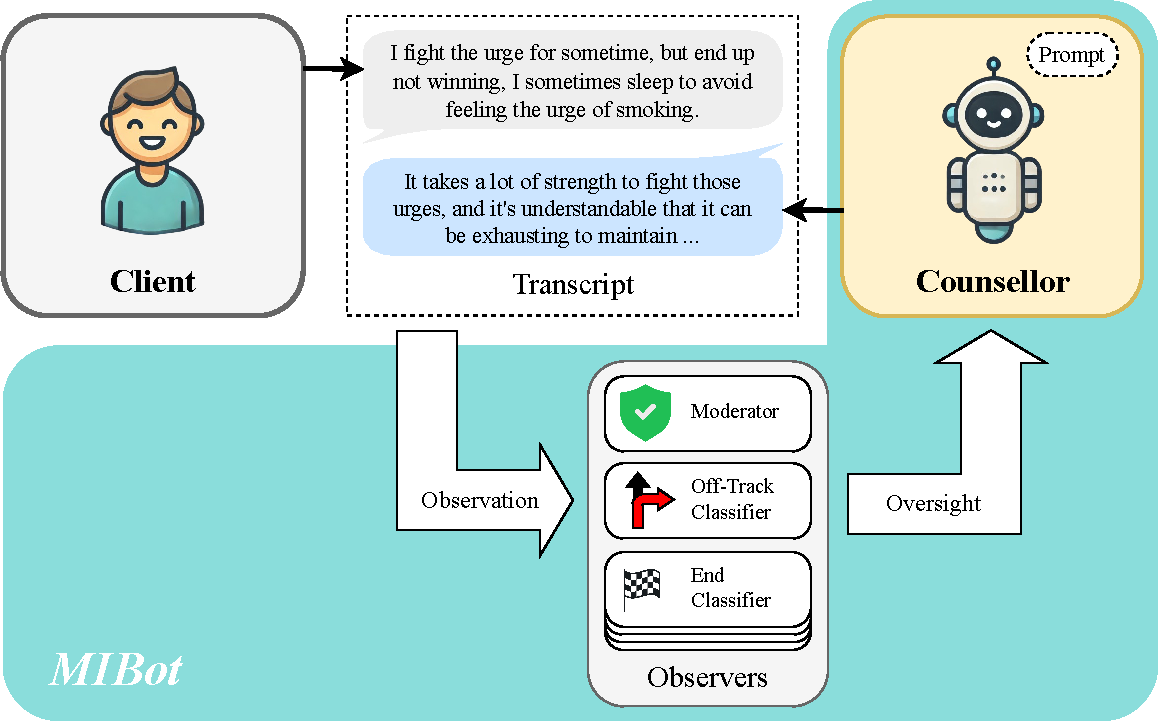
\includegraphics[width=0.9\linewidth]{fig/sysdiag.pdf}
	\caption[Overview of the MIBot system]{Overview of the MIBot system, which includes a core counsellor agent and a set of observer agents for safety and coherence. The system interacts with the user, and the observers monitor the conversation for harm, off-track dialogue, and conversation termination cues. Taken from \citet{mahmood-etal-2025-fully}.}
	\label{fig:sysdiag}
\end{figure}

\section{Observers}
\label{sec:observers}
To improve safety in the deployment of MIBot, the core counsellor agent was supplemented with a set of \textit{observer agents}, independent instances of GPT-4o prompted to monitor specific aspects of the conversation in real time. The output of these agents is used to intervene when necessary. Each observer was specialized through prompt engineering to perform a specific task in real time (see \Cref{app:observer-prompts} for the full prompts).

\subsection{Moderator}
The \textit{Moderator} evaluates the counsellor's most recent utterance for potential harm before it is displayed to the client. While OpenAI's internal safety systems reduce many risks, they do not address all possible counterproductive counselling behaviours, such as inadvertently reinforcing \emph{sustain talk} or suggesting self-harm. The Moderator was intentionally configured for high sensitivity, accepting a higher false positive rate to reduce the risk of harmful or counterproductive content. If a counsellor's utterance is flagged, it is regenerated and re-evaluated, with up to five regeneration attempts permitted. In all study conversations, an acceptable utterance was produced within four attempts, and no session failed to pass moderation.

\subsection{Off-Track Conversation Classifier}
The \textit{Off-Track Classifier} detects when a client is steering the dialogue away from smoking cessation in a deliberate or sustained manner. Its prompt was tuned for low false positive rates to preserve conversational flexibility. In the feasibility study described in \Cref{ch:mibot-feasibility-study}, this observer's primary role was retrospective --- identifying conversations for exclusion where the participant was not engaging seriously with the intervention. In a live deployment, it can be used to trigger early termination or redirection to the main topic.

\subsection{End Classifier \& Termination Process}
The \textit{End Classifier} monitors both parties' dialogue to determine if the conversation is reaching a natural conclusion. It prioritizes the client's intent when making this determination, ensuring the conversation is not ended prematurely. Upon detecting an intent to close, it instructs the counsellor to deliver a concise summary of main discussion points --- a standard MI practice --- and to confirm with the client whether they wish to continue. If the client declines, the conversation is terminated and any post-session procedures, such as surveys, are initiated.


\textbf{Design Rationale:} All observers were implemented as separate, stateless LLM calls, each with prompts tailored to their decision criteria. This modular approach allowed independent improvement of their sensitivity–specificity balance without affecting the primary counsellor prompt. The Moderator favoured recall over precision to err on the side of client safety, whereas the Off-Track Classifier did the opposite, favouring conversational autonomy. The End Classifier's logic explicitly distinguished between topic changes and true conversation endings, reducing false terminations.


The prompted GPT-4o, together with observers, constitute the complete MIBot system, as illustrated in \Cref{fig:sysdiag}.


\section{MIBot System Design}
\label{sec:deployment}


\subsection{Overview of the Application}


MIBot is implemented as a containerized software system that can be run locally for development and deployed to cloud-based systems. In this section, we discuss the implementation details of MIBot, from the structure of the Python microservice and its integration with the OpenAI API to the containerization and the deployment of the service on Amazon Web Services.

The core of MIBot is a lightweight Python web application built with the \texttt{Sanic} framework~\citep{pi_sanic}. In MIBot, \texttt{app.py}, the main entry point, uses \texttt{Sanic} to configure routes for all external interactions and instantiates the conversation engine.
\begin{figure}[ht]
	\centering
	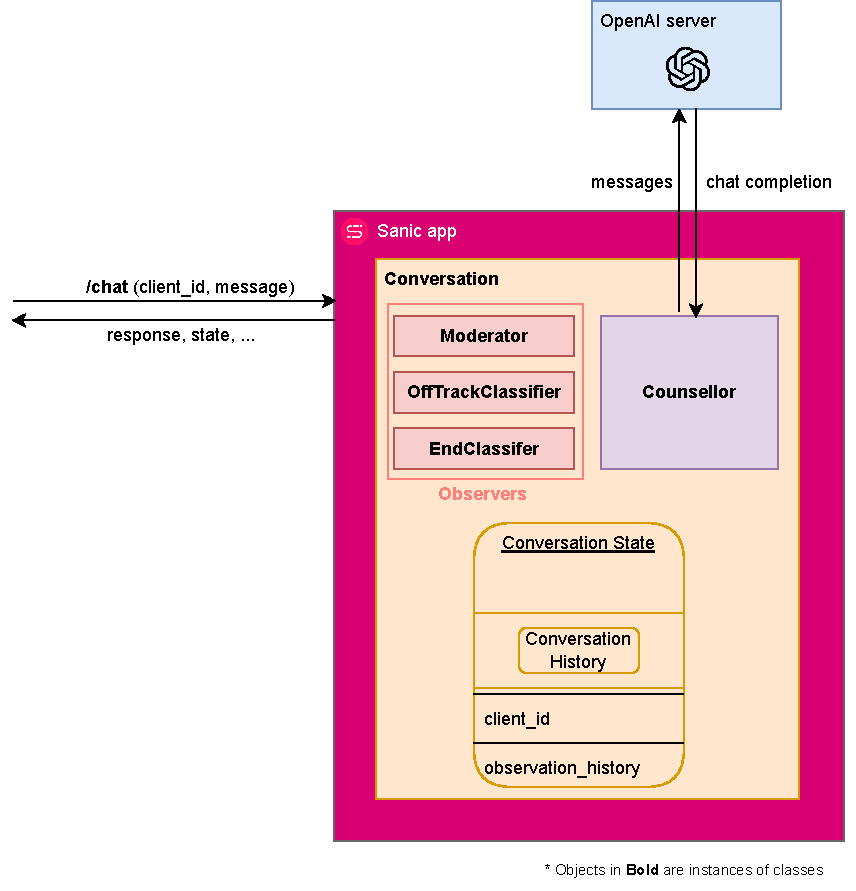
\includegraphics[width=0.7\linewidth]{fig/microservice.drawio.pdf}
	\caption[MIBot Sanic Application Overview]{An overview of the Sanic web application that encapsulates the MIBot code. The application exposes REST APIs for external interactions, such as handling chat messages and providing conversation transcripts.}
	\label{fig:microservice}
\end{figure}
An overview of the application's architecture is presented in \Cref{fig:microservice} (see \Cref{app:architecture-diagrams} for more detailed diagrams). When a user sends a request to the \texttt{/chat} endpoint containing their message and \texttt{client\_id}, the web server updates the state of the conversation and requests the next turn from it. The \texttt{Conversation} object relays this to the \texttt{Counsellor}, which in turn sends a request to the OpenAI API with the accumulated conversation history and the current client message, and receives a response containing the generated counsellor turn.

Each \texttt{Observer} attached to the \texttt{Conversation} inherits from a base class defining an asynchronous \texttt{observe()} method. As noted earlier, the \texttt{Moderator} observer screens counsellor utterances for safety and appropriateness; the \texttt{Off-Track Classifier} observer assesses whether the client is steering the conversation away from smoking cessation; and the \texttt{End Classifier} determines when a session should conclude. These observers are implemented as separate GPT-4o API calls with their own prompts. After each turn, the \texttt{Conversation} object iterates over all \texttt{Observer} objects, collects their observations, and makes real-time decisions (e.g., whether to end the conversation) before updating its state. If the generated output from the \texttt{Counsellor} is deemed suitable for the client, it is sent to the client along with relevant metadata.

A single \texttt{Sanic} app can handle multiple clients at once by creating replicas of the \texttt{Conversation} object, each uniquely identified by the \texttt{client\_id}.\footnote{For the human feasibility study, to keep track of the participants and their conversations, we explicitly use \texttt{prolific\_id} as \texttt{client\_id}. Prolific (\url{www.prolific.com}) is the platform we use to recruit participants and conduct our feasibility study. See Chapter 4 for further details.} The microservice also exposes some additional endpoints: \texttt{/get\_transcript} provides a downloadable transcript of the conversation for post-session analysis; \texttt{/health} returns a simple \texttt{200 OK} response so that load balancers and orchestrators can perform health checks; and \texttt{/info} exposes build metadata such as the current version of the prompt.

\subsection{Containerization}

\begin{figure}[ht]
	\centering
	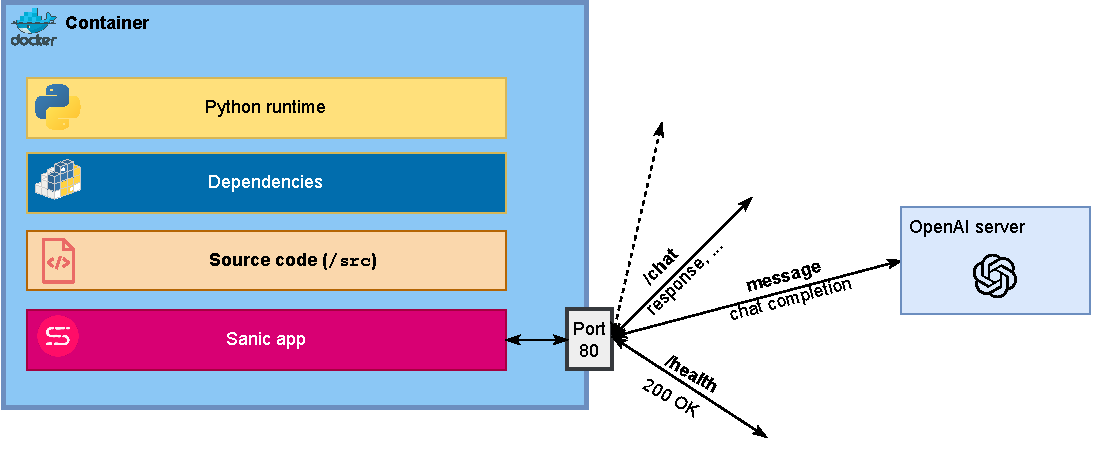
\includegraphics[width=0.7\linewidth]{fig/container.drawio.pdf}
	\caption[Containerized MIBot Application]{The containerized Sanic application for MIBot. The application is packaged in a Docker container for reproducibility and ease of deployment, with the container image stored in Amazon Elastic Container Registry (ECR).}
	\label{fig:containerization}
\end{figure}

For reproducibility and ease of deployment, the microservice is packaged in a Docker container. Containerization provides several advantages for the development, testing, and deployment of MIBot, including environment consistency, portability, isolation, scalability, faster deployment and rollbacks, simplified CI/CD integration, and reproducibility, as discussed in detail by Sloane~\citep{sloane2025containerization}. An overview of the containerized application is presented in \Cref{fig:containerization}.

The MIBot container image is defined by a \texttt{Dockerfile} (see \Cref{app:deployment-artifacts}) specifying the base Python runtime, required dependencies, the source code, and main entry point (viz. \texttt{app.py}). This image is stored in Amazon Elastic Container Registry (ECR). The container registry stores all the images built by the CI/CD pipeline, but only the image with the \texttt{production} tag is used for deployment.

\section{Deploying MIBot to AWS}
\label{sec:mibot-deployment}

MIBot is deployed as a service on Amazon \textbf{Elastic Container Service (ECS)}. ECS is a fully managed service provided by Amazon Web Services (AWS) that ``makes easier the deployment, management, and scaling of applications using containers''~\citep{aws-ecs-getting-started}. We now discuss each component of ECS.

\subsection{Components of ECS}
An overview of the deployment architecture is presented in \Cref{fig:ecs-components}.
\begin{figure}[ht]
	\centering
	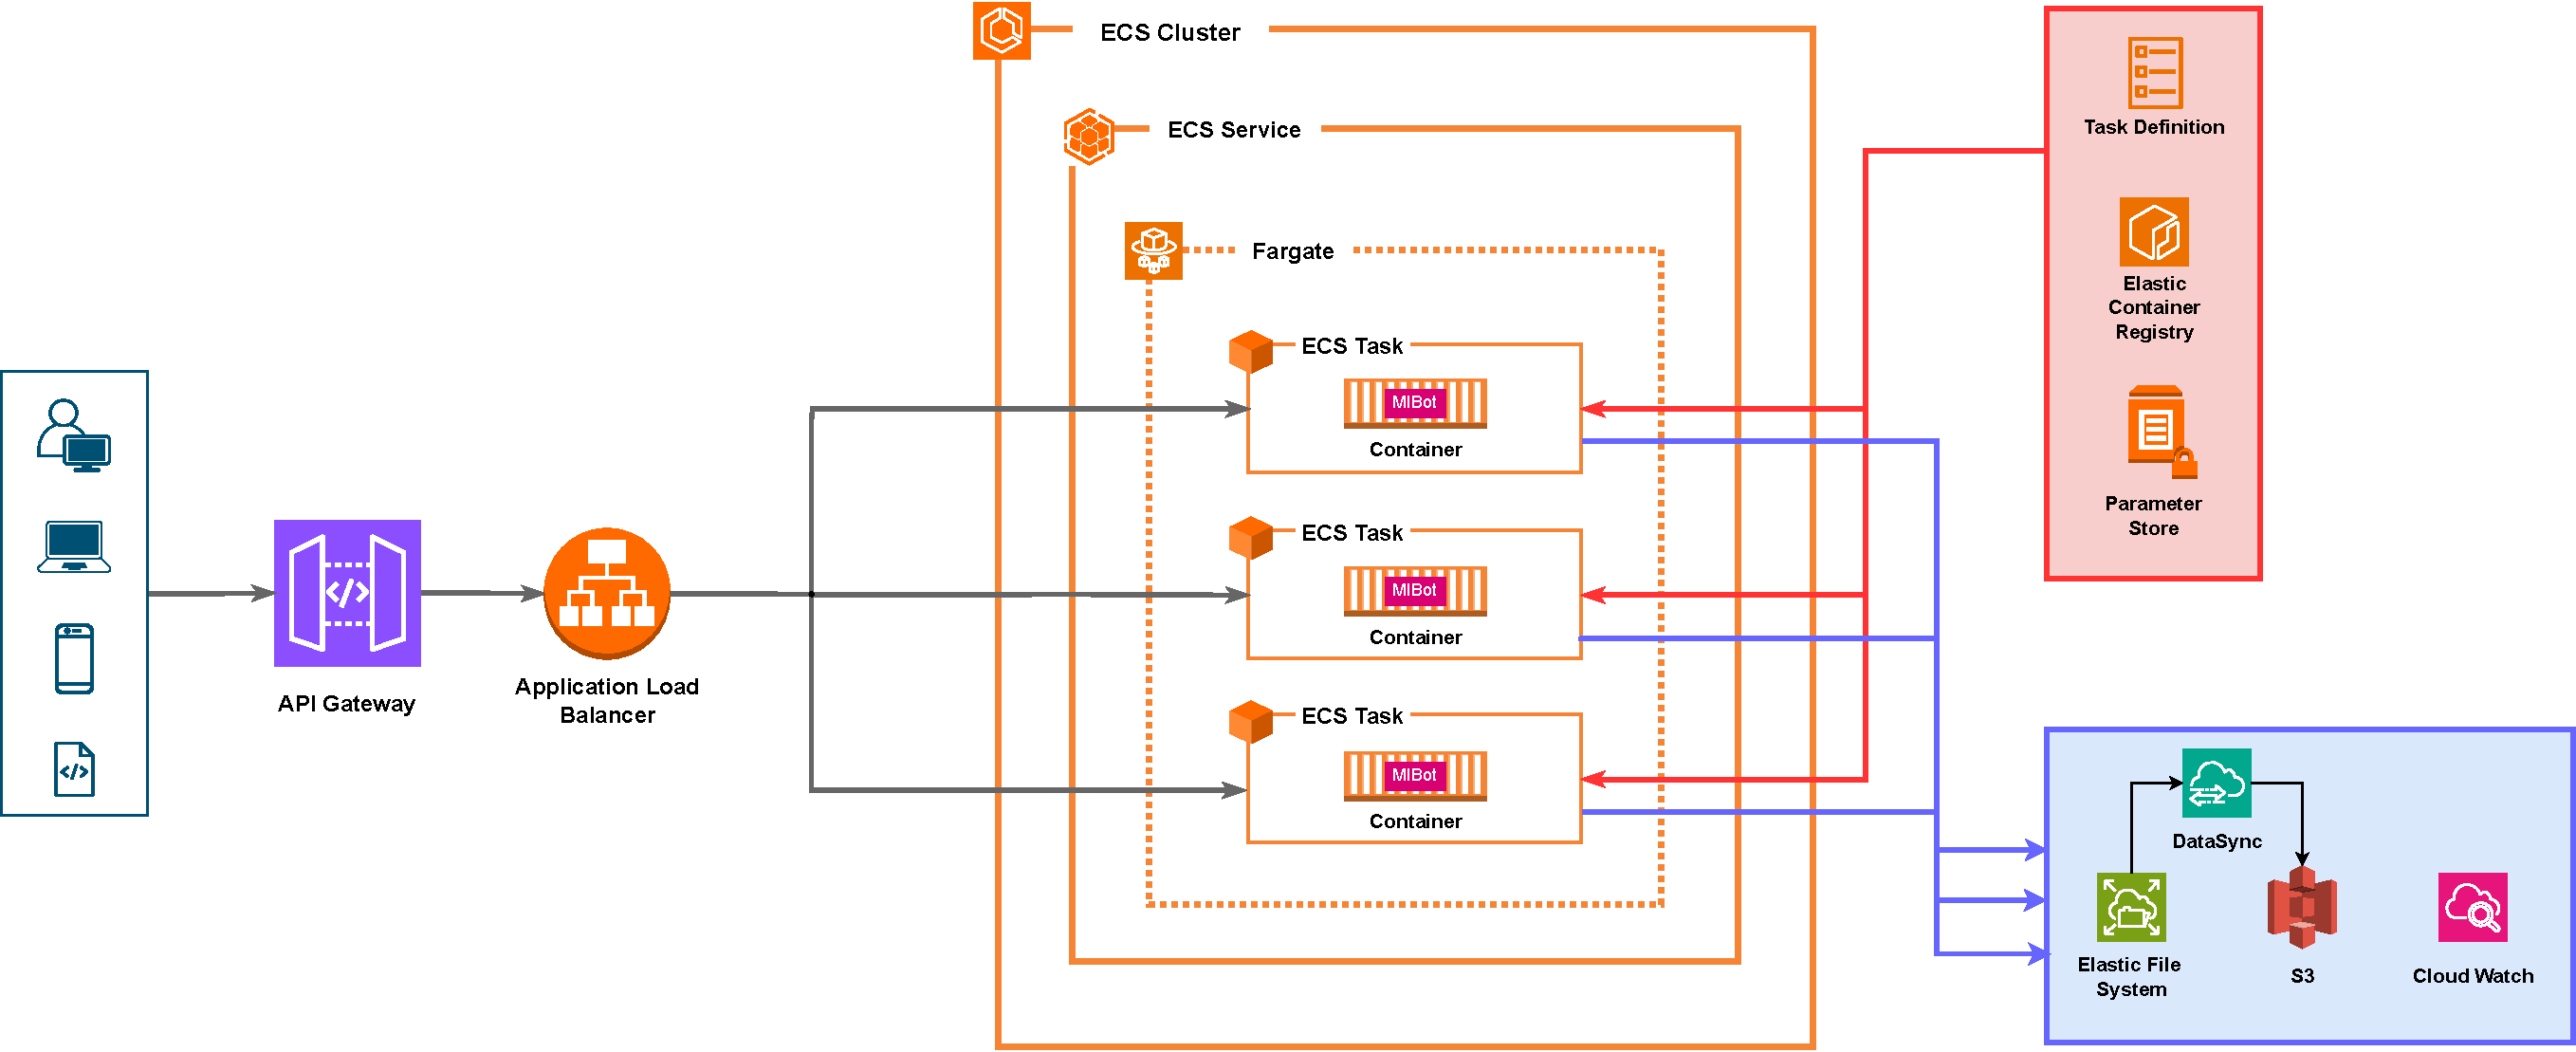
\includegraphics[width=0.99\linewidth]{fig/deployment.drawio.pdf}
	\caption[MIBot Deployment on AWS ECS]{An overview of the deployment of the containerized MIBot application on Amazon Elastic Container Service (ECS). The diagram shows the key components, including the ECS cluster, the ECS service, and the ECS task definition, as well as the interaction with other AWS services like Elastic Load Balancer (ELB) and API Gateway.}
	\label{fig:ecs-components}
\end{figure}

\paragraph{1. ECS Cluster} to deploy MIBot to ECS, we first provisioned an \textbf{ECS cluster} (\texttt{mibot-v6-cluster}). An ECS cluster is a \textit{logical} grouping of heterogeneous compute resources. In the context of AWS, a \textbf{compute resource} is any AWS-managed infrastructure component that provides processing power for running applications or workloads. These resources can be \textbf{user-managed}, like Elastic Compute Cloud (EC2), where users rent virtual machines, or \textbf{fully managed}, like AWS Fargate, which is used to run containerized applications without direct server management. A cluster is therefore a logical grouping of such compute resources.

In our ECS cluster, however, we only used \textbf{AWS Fargate} as the computing resource. In addition to allowing for the deployment of the containerized MIBot application without server management, AWS Fargate also offers \emph{spot runs} for cost optimization. In the \texttt{FARGATE\_SPOT} mode, tasks run on spare compute capacity. If a container receives no traffic in the last two hours and AWS reclaims the capacity, the task will be terminated. ECS will detect this event and will almost immediately instantiate a new task for the application.

\paragraph{2. ECS Service} Inside the ECS cluster, we created an \textbf{ECS Service} (\texttt{mibot-v6-service}). The ECS Service contains the deployment configuration of the application, for example, the number of desired replicas of the application (also called \emph{tasks}) that should run at any given time.  For our study, we set this to use two tasks. If one of the tasks fails, the ECS Service replaces it automatically. It can also be configured to increase the number of tasks when it detects higher-than-normal traffic. The Service is connected to an Elastic Load Balancer (ELB) to distribute incoming traffic evenly among tasks. It also defines deployment (rolling update, blue/green deployment) and rollback strategies, and can use the AWS circuit breaker to roll back failed deployments automatically.

\paragraph{3. ECS Task Definition} The final component in the deployment of MIBot is defining a \textbf{Task}. A \texttt{Task} runs a specific container after downloading it from the Elastic Container Registry (ECR). The \texttt{Task} definition specifies environment variables and API credentials that are securely stored in AWS Systems Manager Parameter Store and are injected into the container (e.g., \texttt{OPENAI\_API\_KEY}) when the task is started. It further defines a \emph{health check} for the container. The health check sends a request to the \texttt{/health} endpoint on the container's port~80 every five minutes. If the response is anything other than \texttt{200 OK} or it does not get a response within one minute, it deems the container unhealthy. The \texttt{Service} terminates the \texttt{Task} and replaces it with a new one. The task definition further specifies the required CPU and memory (1024 CPU units (1 vCPU) and 4~GB, respectively, in the case of MIBot). The containers also mount a persistent Amazon Elastic File System (EFS) volume to store conversation transcripts and evaluation metrics. Furthermore, all container logs are written to AWS CloudWatch for retrospective analysis of the system's behaviour.

\subsection{Other Components of the Deployment}

\paragraph{Load Balancer} We configured an Elastic Load Balancer (\texttt{mibot-elb}) with three subnets for high availability, with three instances of load balancers in three different Availability Zones. The load balancers are \emph{application} load balancers (ALB)~\citep{aws_alb}, which are internet-facing and associated with a security group permitting inbound traffic on port 443. The DNS names allow external users to connect to the service through a custom domain name~\citep{shopify_domain_seo}. The ALB routes incoming HTTP requests to the ECS service's target group and internal health check requests to the \texttt{/health} endpoint.

\paragraph{API Gateway} We also provisioned an AWS API Gateway, which acts as a reverse proxy and enables secure TLS termination and request throttling. The gateway exposes HTTPS endpoints for \texttt{/chat}, \texttt{/get\_transcript}, \texttt{/health}, \texttt{/info}, and \texttt{/s3\_upload}. Each path includes \texttt{OPTIONS} methods to enable cross-origin requests and defines the expected response headers. This prevents client browsers from blocking requests due to Cross-Origin Resource Sharing (CORS) policies or displaying security warnings.

\paragraph{DataSync} Conversation transcripts and metadata are stored on both an encrypted EFS volume and AWS S3 only when the participant clicks on the final Submit button at the end of the study session. EFS acts as a redundant data layer in case the upload to S3 fails. For eventual consistency, we periodically copy files from EFS to S3 using AWS DataSync, which runs a daily CRON job.

\subsection{Deployment Pipeline}
We adopted DevOps practices for automated deployment. Every time we push a special \texttt{production} Git tag to the remote main branch, a GitHub workflow builds the Docker image, runs unit tests, and, if tests pass, pushes the image to Amazon ECR. Another workflow triggers a CloudFormation deployment that updates the ECS task definition with the new image tag and performs a rolling deployment of the ECS Service. Deployment uses a circuit breaker configuration: if the service fails health checks, the rollout is automatically rolled back to the previous stable revision. By integrating the deployment pipeline into version control, we ensured automated deployments tied to code changes.

\chapter{Evaluation of MIBot: Design of the Human Feasibility Study}
\label{ch:feasibility}
The deployed MIBot system was used in a feasibility study with human smokers. The goal of the study was to determine the impact of a single-session interaction with MIBot and assess its safety for delivery to ambivalent smokers in a real-world setting.

\section{Ethics Approval and Consent}
The protocol was approved by the University of Toronto Research Ethics Board under protocol number 49997 (approved August~3, 2024) and adhered to all institutional guidelines. Before participating in the study, prospective participants reviewed an online consent form that outlined study aims, procedures, compensation, potential risks, and data handling practices. Participation required explicit electronic consent. Risks were described as minimal but included the possibility that discussing smoking could cause stress or temporarily increase cravings. No personally identifying information was collected, and all data were de-identified prior to release.

\section{Participant Recruitment}
\label{sec:recruitment}
Participants were recruited via \textit{Prolific}\footnote{\url{https://www.prolific.com}}, an online behavioural research platform with pre-screened participant pools and built-in demographic filters. Prolific was chosen for its ability to target recruitment to specific smoking status, demographic characteristics, and quality-control thresholds, and for its established use in prior MI chatbot studies~\citep{brown2023motivational,info:doi/10.2196/20251}. Participants received \pounds5.50 for the main session and \pounds1.00 for the follow-up survey, exceeding Prolific's recommended hourly rates.


\section{Initial Screening Criteria}
Eligibility screening was implemented at two levels: (1) \textit{Prolific} prescreen filters, applied before invitation to the study; and (2) an in-study screening step prior to chatbot interaction. The first set of filters required that all invitees be 18 years or older, be fluent in English, have an approval rate of at least 90\% on prior Prolific studies and self-identify as a \emph{current smoker} of at least five cigarettes per day, with a history of smoking at this rate for one year or more.

In addition, recruitment was set up to aim for a nearly equal sex balance. Although the final sample reflected slight deviations due to subsequent exclusion filtering, this pre-allocation ensured coverage across male and female participants.

\section{In-Study Screening}

\noindent Baseline demographics of enrolled participants are summarized in Table~\ref{tab:participant-characteristics}. All were English-speaking adults who self-identified as current daily smokers and passed prescreening and in-study eligibility checks on Prolific. The sample was approximately sex-balanced with broad age coverage. Residence was primarily the United Kingdom and United States, with additional participants from Canada and South Africa. Unless otherwise specified, values are presented as counts (n) and percentages (%). Age is reported as median, mean (SD), and range.

\section{Participant Characteristics}
\label{subsec:participant-characteristics}
\begin{table}[htbp]
\centering
\caption[Baseline Characteristics of Enrolled Participants]{Baseline characteristics of the 106 enrolled participants in the feasibility study. The table includes demographic information such as sex, age, ethnicity, student and employment status, and country of residence and birth.}
\begin{tabular}{l l}
\hline
\textbf{Characteristic} & \textbf{n (\%)} \\
\hline
Total participants & 106 \\
\hline
Sex & \\
\quad Female & 57 (53.8) \\
\quad Male & 49 (46.2) \\
\hline
Language & \\
\quad English-speaking & 106 \\
\hline
Age summary & Range 22--77; median 38; mean 40 (SD 13) \\
Age groups (years) & \\
\quad Below 20 & 0 (0.0) \\
\quad 20 to 29 & 26 (24.5) \\
\quad 30 to 39 & 32 (30.2) \\
\quad 40 to 49 & 20 (18.9) \\
\quad 50 to 59 & 19 (17.9) \\
\quad 60 to 69 & 6 (5.7) \\
\quad 70 to 79 & 3 (2.8) \\
\quad Above 79 & 0 (0.0) \\
\hline
Ethnicity & \\
\quad White & 80 (75.5) \\
\quad Black & 9 (8.5) \\
\quad Asian & 7 (6.6) \\
\quad Mixed & 5 (4.7) \\
\quad Other & 5 (4.7) \\
\hline
Student status & \\
\quad No & 80 (75.5) \\
\quad Yes & 21 (19.8) \\
\quad Data expired & 5 (4.7) \\
\hline
Employment status & \\
\quad Full-time & 49 (46.2) \\
\quad Part-time & 18 (17.0) \\
\quad Not in paid work & 16 (15.1) \\
\quad Unemployed & 13 (12.3) \\
\quad Other & 10 (9.4) \\
\hline
Country of residence & \\
\quad United Kingdom & 47 (44.3) \\
\quad United States & 42 (39.6) \\
\quad Canada & 9 (8.5) \\
\quad South Africa & 4 (3.8) \\
\quad Other & 4 (3.8) \\
\hline
Country of birth & \\
\quad United Kingdom & 44 (41.5) \\
\quad United States & 39 (36.8) \\
\quad Canada & 6 (5.7) \\
\quad Kenya & 3 (2.8) \\
\quad South Africa & 3 (2.8) \\
\quad Germany & 2 (1.9) \\
\quad Other & 9 (8.5) \\
\hline
\end{tabular}
\label{tab:participant-characteristics}
\end{table}


Upon accessing the study website, participants completed a smoking status confirmation question identical to Prolific's prescreen question. From an initial pool of 159 participants, we screened for ambivalence using the \textit{Readiness Ruler}, as described in Section~\ref{subsec:readiness-ruler}. To ensure participants were in a state where MI could be beneficial, we included those with a pre-conversation \emph{confidence-to-quit} score of 5 or less on a 10-point scale. We also included 'discordant'
participants, who, despite having high confidence (a score greater than 5), rated the importance of quitting at least five points lower than their confidence. This process resulted in a final sample of 106 participants.


Participants who met all criteria and provided informed consent proceeded to the survey phase. Those who did not meet the eligibility criteria were redirected to the Prolific platform without completing the study.

\section{Study Procedure}
\begin{figure}[ht]
    \centering
    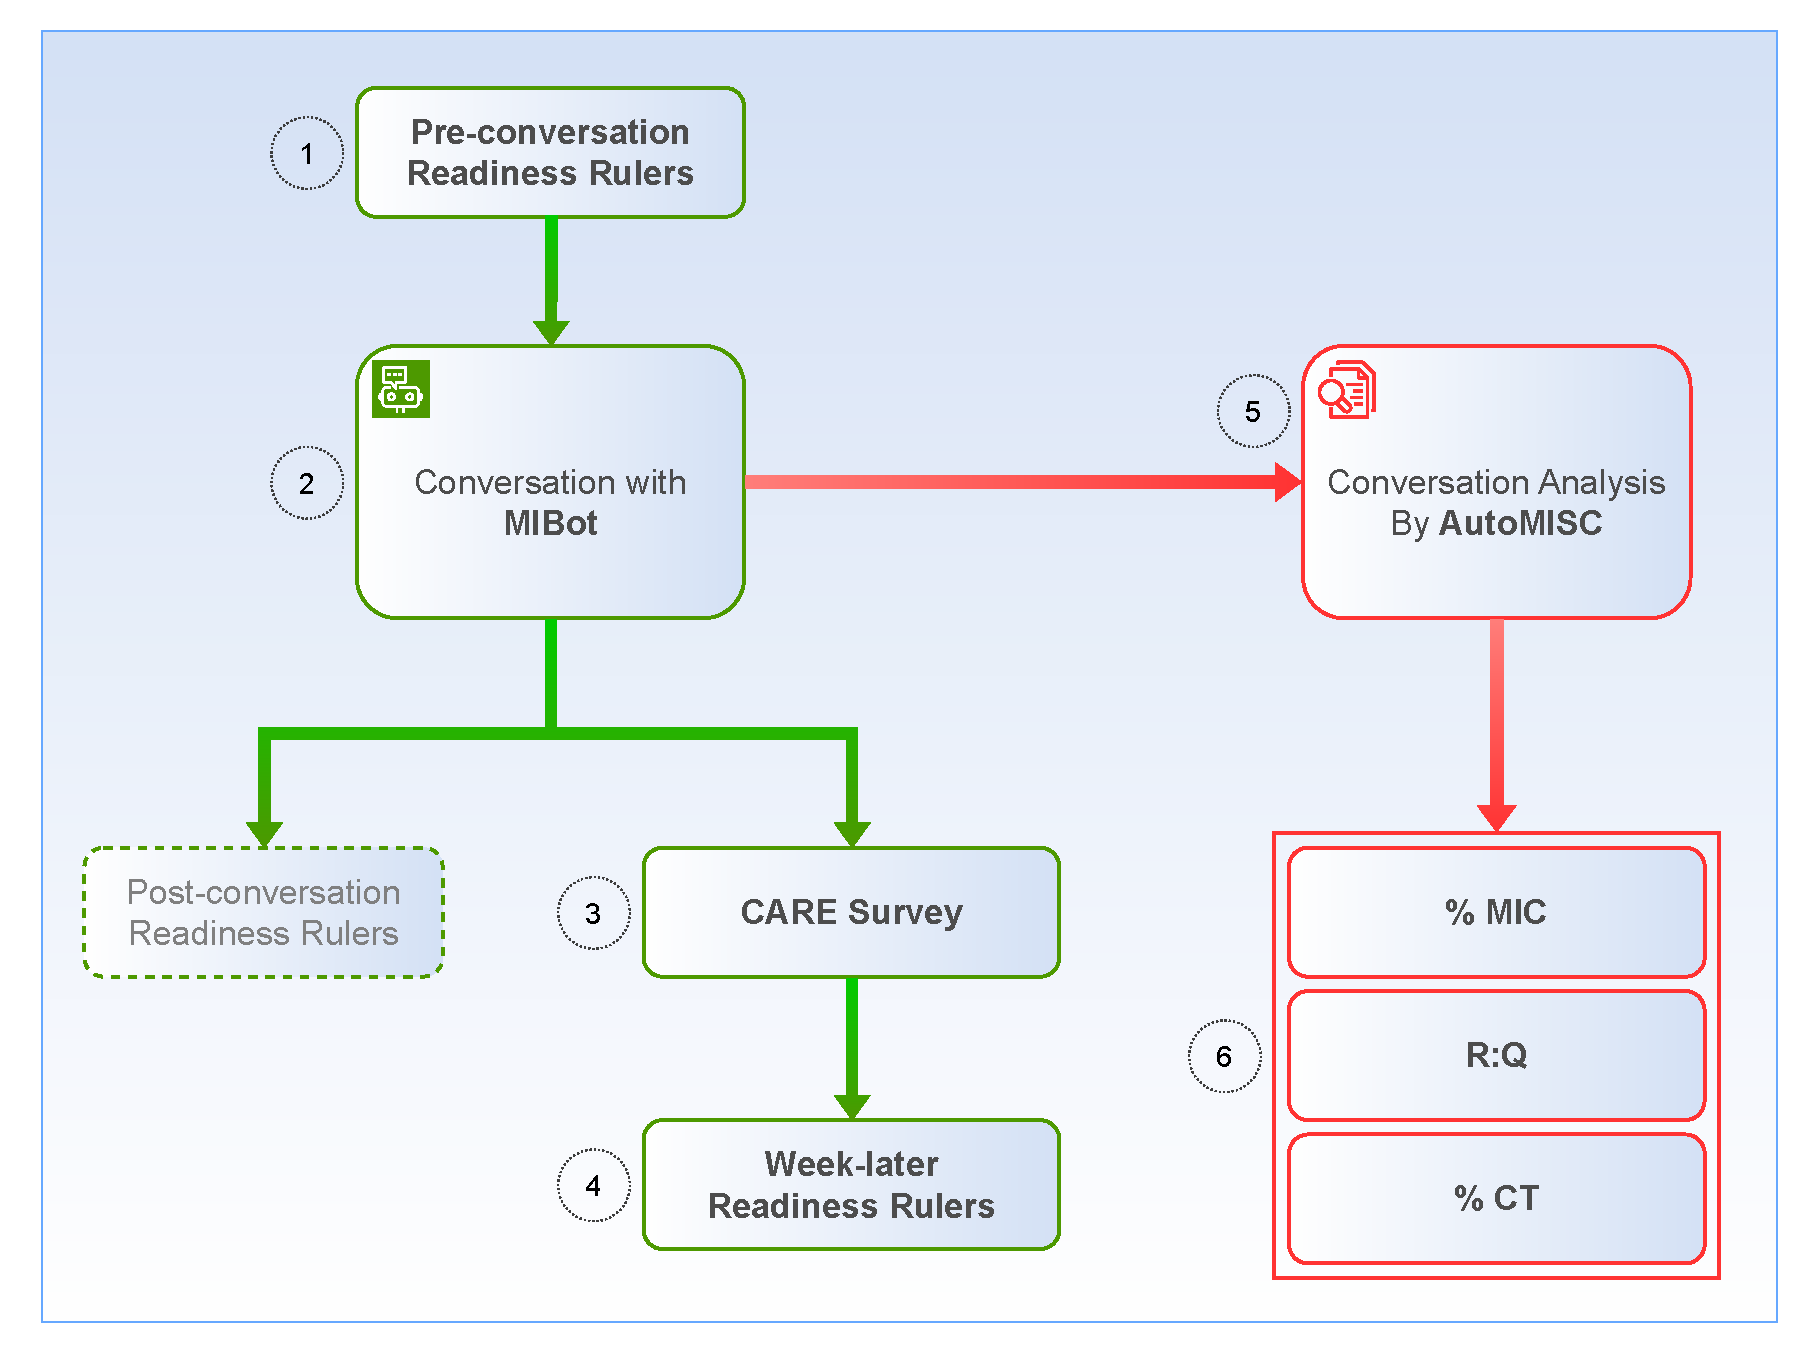
\includegraphics[width=0.9\linewidth]{fig/feasibility_study_flow.pdf}
    \caption[Feasibility Study Protocol Overview]{Overview of the feasibility study protocol, illustrating the four main phases: pre-conversation surveys, a single text-based conversation with MIBot, immediate post-conversation surveys, and a one-week follow-up survey.}
    \label{fig:study-flow}
\end{figure}

The full study procedure comprised four major phases: (1) pre-conversation surveys; (2) a single text-based conversation with MIBot; (3) immediate post-conversation surveys; and (4) a one-week follow-up survey. Figure~\ref{fig:study-flow} illustrates the progression.



\paragraph{Phase 1: Pre-Conversation Surveys:}
Before interaction with MIBot, participants completed:
\begin{enumerate}
    \item \textbf{Heaviness of Smoking Index (HSI)}~\citep{heatherton1989measuring} survey, which assesses nicotine dependence via two questions:
        \begin{enumerate}
            \item number of cigarettes smoked per day (scored 0-3), and
            \item time to first cigarette after waking (scored 0-3).
        \end{enumerate}
    The HSI score is the sum of these two items, and ranges from 0 to 6, with higher scores indicating greater nicotine dependence.
    \item \textbf{Quit Attempts in the Past Week}: number of conscious attempts to abstain from smoking for at least 24 hours during the preceding seven days.
    \item \textbf{Readiness Ruler}: three questions measuring self-reported ratings of importance, confidence, and readiness to quit on 0–10 scales (Section~\ref{subsec:readiness-ruler}).
\end{enumerate}

\paragraph{Phase 2: Conversation with MIBot:}
Participants engaged in a single MI-style conversation via a web-based text interface.

\paragraph{Phase 3: Post-Conversation Surveys:}
Immediately after the conversation, participants repeated the Readiness Ruler, completed the CARE empathy scale (Section~\ref{subsec:care}), and provided qualitative feedback on the chatbot's performance.

\paragraph{Phase 4: One-Week Follow-Up:}
Seven days later, participants were invited via Prolific to complete a follow-up survey. This included a third administration of the Readiness Ruler and questions about quit attempts and changes in smoking behaviour over the past week.

\section{Survey Instruments}
\label{subsec:survey-instruments}

The goal of the work is to move ambivalent smokers towards the decision to quit. We employed the following metrics to measure outcomes from the interaction. In addition to the primary outcome measures, we also recorded other survey instruments to get a holistic picture of the chatbot's effectiveness.

\subsection{1. Readiness Ruler}
\label{subsec:readiness-ruler}
The Readiness Ruler~\citep{rollnick1992development} is a validated tool for assessing motivational state across three dimensions:
\begin{itemize}
    \item \textbf{Importance:} ``How important is it to you right now to stop smoking?''
    \item \textbf{Confidence:} ``How confident are you that you would succeed at stopping smoking if you started now?''
    \item \textbf{Readiness:} ``How ready are you to start making a change at stopping smoking right now?''
\end{itemize}
Responses were recorded on an 11-point scale (0 = ``not at all'', 10 = ``extremely''). The week-later change in \emph{confidence} from the pre-conversation value was used as the primary metric for the chatbot's effectiveness, as this is the most predictive
of downstream quitting success~\cite{Gwaltney2009-wj,Abar2013}.

\subsection{2. CARE Measure}
\label{subsec:care}
The Consultation and Relational Empathy (CARE) measure~\citep{10.1093/fampra/cmh621,Bikker2015} assesses perceived empathy in clinical encounters. Ten items evaluate the counsellor's ability to make the participant feel at ease, listen actively, appreciate the participant as a whole person, and collaborate on problem-solving. Each question is rated on a 0-5 scale, with a total score range of 0-50.

\subsection{3. Qualitative Feedback}
Three open-ended questions solicited subjective impressions:
\begin{enumerate}
    \item ``What are three words that you would use to describe the chatbot?''
    \item ``What would you change about the conversation?''
    \item ``Did the conversation help you realize anything about your smoking behaviour? Why or why not?''
\end{enumerate}
These responses can inform future prompt refinements and provide contextual data for interpreting quantitative outcomes.

\subsubsection{4. Follow-Up Quit Attempt Survey}
At one week, participants reported whether they had made any quit attempts in the preceding seven days, the number of attempts, and whether any changes in smoking habits had occurred. This included partial changes, such as a reduction in cigarettes per day.

\section{Automated Conversation Analysis}
\label{subsec:automisc}
In addition to participant-reported outcomes, conversations were analyzed for MI adherence and elicitation of motivational language using \textit{AutoMISC}, an automated implementation of the Motivational Interviewing Skill Code v2.5~\citep{Houck2010}. The AutoMISC system was primarily developed by Soliman, as described in his thesis [CITE\_THESIS], with further validation in~\cite{ali2025automated}. For this project, we utilized the existing AutoMISC system and contributed to the work described in~\cite{mahmood-etal-2025-fully}. The analysis pipeline first segments each conversational volley into individual utterances. Then, it classifies counsellor utterances as MI-Consistent, MI-Inconsistent, Reflection, Question, or Other. Similarly, it classifies each client utterance as exhibiting Change Talk, Sustain Talk, or Neutral. Finally, it computes the following: \%~MI-Consistent Responses (\%MIC), Reflection-to-Question Ratio (R:Q), \%~Client Change Talk (\%CT). AutoMISC was validated against human coders, including two MI-expert clinicians \cite{mahmood-etal-2025-fully}.


Readiness rulers (especially the week-later change in \emph{confidence}), CARE, and AutoMISC summary metrics together provide a holistic view of the MIBot intervention, assessing its effectiveness, perceived empathy, safety, and adherence to MI principles. In the next chapter, we report the results from our human feasibility study on these metrics.
\chapter{Evaluation of MIBot: Results from the Human Feasibility Study}
\label{ch:mibot-eval}

This chapter presents a comprehensive evaluation of MIBot's effectiveness through a feasibility study with 106 smokers. Building on the system design and implementation described in previous chapters, we assess MIBot's performance across four critical dimensions established in the smoking cessation and motivational interviewing literature: behavioural change readiness, perceived therapeutic empathy, adherence to MI principles, and elicitation of client change talk.

The chapter is organized to progress from primary outcomes through measurements of therapeutic process, and finally, to behavioural changes and user experiences. First, we report the primary outcome of changes in readiness to quit smoking (Section~\ref{sec:primary-outcome}). We then analyse how the chatbot performed on perceived empathy, measured through the CARE scale and compare it to human healthcare professionals (Section~\ref{sec:perceived-empathy}). Next, we examine MIBot's adherence to MI principles through AutoMISC analysis, and examine if MIBot could maintain fidelity to therapeutic standards while successfully eliciting change talk from clients (Section~\ref{sec:mi-adherence}).

Following these core metrics, we investigate behavioural outcomes including quit attempts and self-reported changes (Section~\ref{sec:behavioural-outcomes}), explore conversation dynamics both quantitatively and qualitatively (Section~\ref{sec:conversation-dynamics}), and examine illustrative case studies and sample outliers (Section~\ref{sec:case-studies}). Finally, we analyse participant feedback (Section~\ref{sec:feedback}) and discuss broader implications of our findings (Section~\ref{sec:synthesis}).

\section{Primary Outcome: Readiness to Quit}
\label{sec:primary-outcome}

\subsection*{Overall Changes in Readiness Rulers}

Table~\ref{table:mibot_ruler_summary} summarizes the mean (and standard deviation) of each readiness ruler before the conversation, immediately afterwards, and one week later. The table includes the change between the pre-conversation metric and one week later ($\Delta$). The Wilcoxon signed-rank test was applied to assess the significance of the change. Participants' confidence increased markedly from a baseline mean of 2.8 to 4.5 one week later ($\Delta=1.7$, $p<10^{-9}$). This represents a $\sim$59\% relative improvement and constitutes our primary outcome measure, aligning with MI theory that confidence (self-efficacy) is a key predictor of behaviour change \citep{Gwaltney2009-wj,Abar2013}. Importance also increased, albeit more modestly ($\Delta=0.5$, $p<0.005$), while readiness exhibited a small, non-significant change ($\Delta=0.3$, $p=0.22$).

\begin{table}[ht!]
  \centering
  \small
  \setlength{\tabcolsep}{4pt}
  \renewcommand{\arraystretch}{1.1}
  \begin{tabular}{@{}lcccc@{}}
    \toprule
    \textbf{Ruler} & \textbf{Before} & \textbf{After} & \textbf{One Week} & \textbf{$\Delta$} \\
    & \textbf{mean (SD)} & \textbf{mean (SD)} & \textbf{mean (SD)} & \textbf{mean (SD)} \\
    \midrule
    Importance & 5.7 (2.6) & 6.3 (2.9) & 6.1 (2.7) & 0.5 (1.7)** \\
    Confidence & 2.8 (2.0) & 4.6 (2.6) & 4.5 (2.7) & 1.7 (2.4)*** \\
    Readiness  & 5.2 (2.8) & 5.9 (2.8) & 5.5 (3.0) & 0.3 (2.4) \\
    \bottomrule
  \end{tabular}
  \caption[MIBot Readiness Ruler Summary]{Means and standard deviations (SD) of readiness rulers (0--10 scale) for importance, confidence, and readiness, measured at three time points: before the conversation, immediately after, and one week later. The table also shows the mean change ($\Delta$) between the pre-conversation measurement and the one-week follow-up. Statistical significance of the change is assessed using the Wilcoxon signed-rank test (*** $p < 0.001$, ** $p < 0.01$, * $p < 0.05$).}
  \label{table:mibot_ruler_summary}
\end{table}

Figure~\ref{fig:confidence_change_distribution} illustrates the distribution of one-week changes in confidence. Of the 106 participants, 64 (60.4\%) showed improvement, 21 (19.8\%) remained unchanged, and 21 (19.8\%) experienced a decrease. The median change was +1.0 point, with the interquartile range spanning 0 to +3 points. Notably, 15 participants (14.2\%) achieved gains of 5 or more points, representing substantial movement toward quitting confidence.

\begin{figure}[ht]
  \centering
  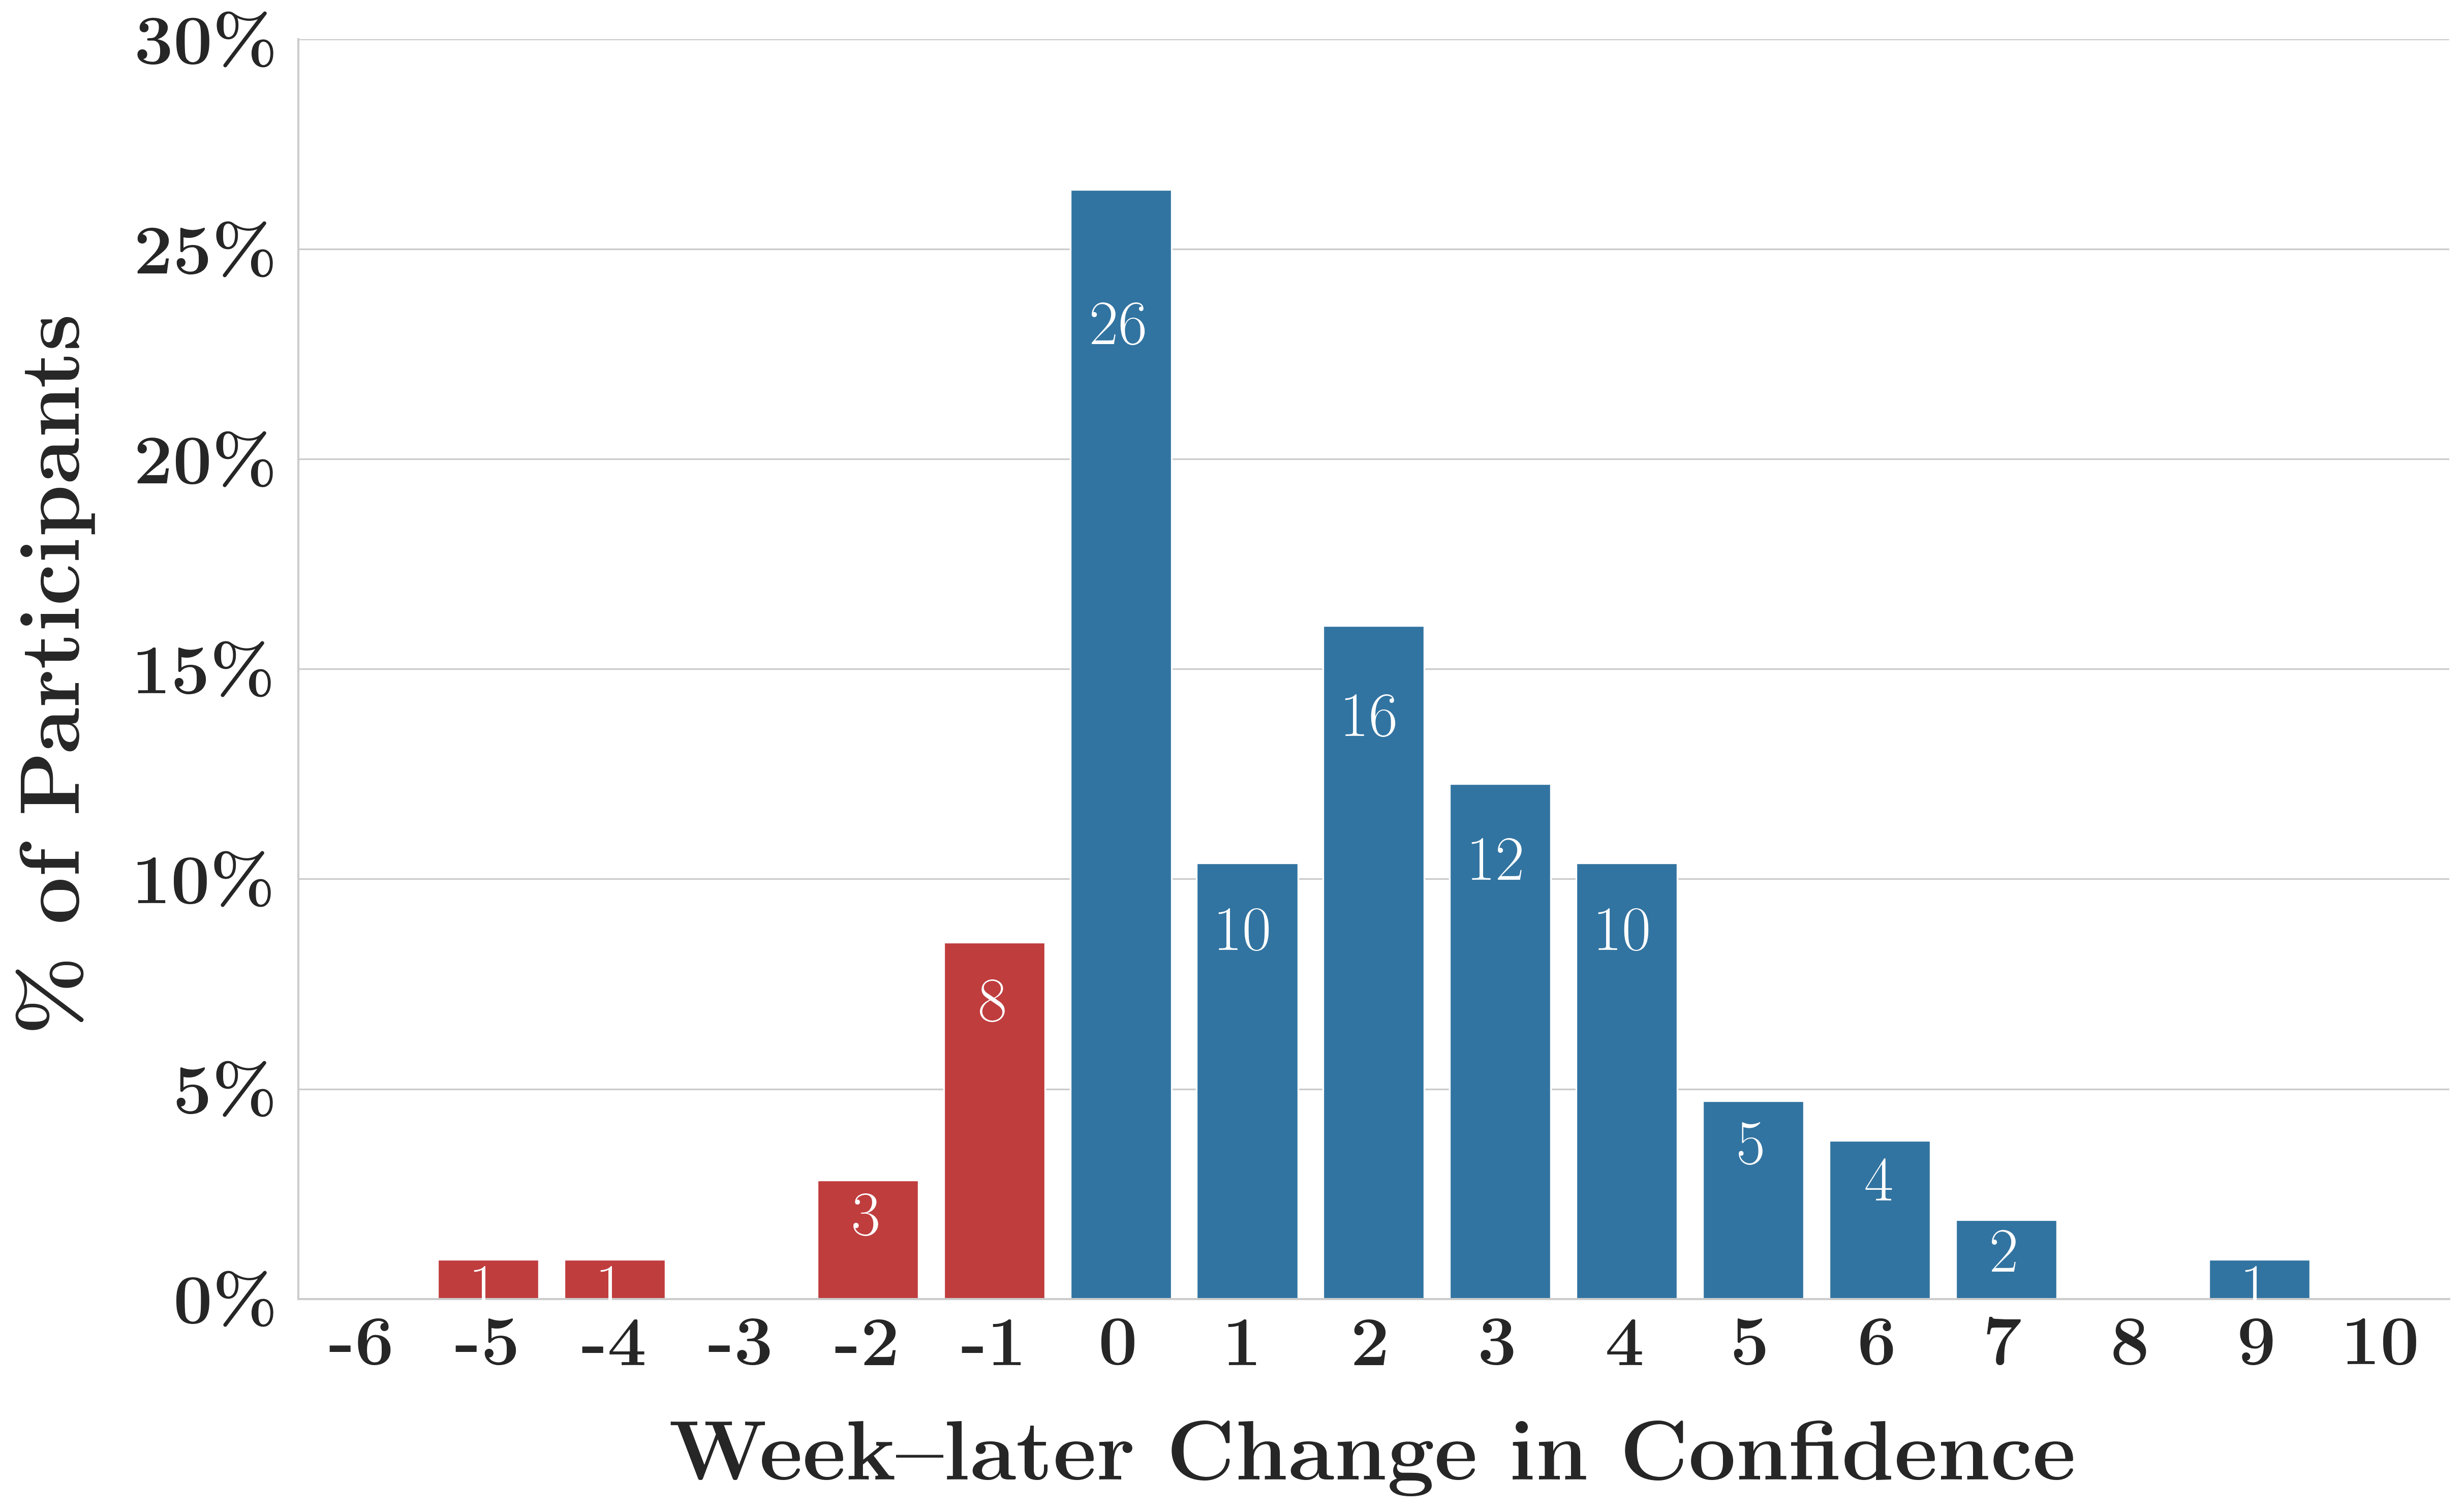
\includegraphics[width=0.8\linewidth]{fig/2024-11-14-MIV6.3A-2024-11-22-MIV6.3A_ruler_deltas_delta_with_week_later_keep_high_conf_False_change.png}
  \caption[Distribution of Confidence Changes]{Distribution of one-week changes in confidence scores (post-conversation minus pre-conversation). The x-axis represents the change in confidence on a 0-10 scale, and the y-axis represents the number of participants. The majority of participants (60.4\%) showed an improvement in confidence.}
  \label{fig:confidence_change_distribution}
\end{figure}



\subsection*{Stratified Analysis by Baseline Characteristics}

To understand which participants benefited most from MIBot, we stratified outcomes by baseline characteristics. Table~\ref{tab:baseline_confidence} shows that those starting with the lowest self-confidence ($n=31$, confidence $\leq 1$) experienced the largest improvement (+2.2 points), whereas participants with moderate or higher confidence gained about one and a half points. The three participants who began with very high confidence showed a decline, likely reflecting regression to the mean. Baseline confidence correlated negatively with the change (Spearman $r=-0.21$, $p<0.05$), indicating that MIBot is most beneficial for participants who are least confident in their ability to quit.

\begin{table}[ht!]
  \centering
  \small
  \renewcommand{\arraystretch}{1.1}
  \begin{tabular*}{\linewidth}{@{\extracolsep{\fill}}lccccc@{}}
    \toprule
    \textbf{Baseline} & \textbf{Sample} & \textbf{Baseline} & \textbf{Post-} & \textbf{1-week} & \textbf{Change from} \\
    \textbf{confidence range} & \textbf{size} & \textbf{confidence} & \textbf{conversation} & \textbf{follow-up} & \textbf{baseline} \\
    & & \textbf{mean (SD)} & \textbf{mean} & \textbf{mean (SD)} & \textbf{mean (SD)} \\
    \midrule
    0--1   & 31 & 0.5 (0.5) & 2.7 & 2.7 (2.5) & +2.2 (2.4)*** \\
    2--3   & 32 & 2.5 (0.5) & 2.0 & 4.2 (2.6) & +1.7 (2.5)** \\
    4--5   & 40 & 4.3 (0.5) & 1.4 & 5.8 (2.0) & +1.5 (2.1)*** \\
    $\geq$6 & 3 & 9.3 (0.6) & 0.6 & 7.7 (3.2) & $-1.7$ (2.9) \\
    \bottomrule
  \end{tabular*}
  \caption[Confidence Changes by Baseline Confidence]{Longitudinal changes in self-reported confidence scores (0--10 scale), stratified by baseline confidence level. The table shows the mean confidence scores at baseline, immediately post-conversation, and at 1-week follow-up, for different subgroups of participants based on their initial confidence. The change from baseline to 1-week follow-up is also presented. Statistical significance is determined by the Wilcoxon signed-rank test.}
  \label{tab:baseline_confidence}
\end{table}




Confidence changes varied across different smoking characteristics and quit history profiles. Participants were grouped by HSI (low 0--1, moderate 2--3, high 4--5, very high $\geq$6), daily cigarette consumption ($<$5, 5--9, 10--19, $\geq$20), whether they had made a quit attempt in the week before the study, and the number of prior attempts (0, 1--2, $\geq$3). The mean change in confidence for each subgroup is summarized in Table~\ref{tab:hsi_prequit}.

\begin{table}[ht!]
  \centering
  \small
  \renewcommand{\arraystretch}{1.1}
  \begin{tabular*}{\linewidth}{@{\extracolsep{\fill}}lccccc@{}}
    \toprule
    \textbf{Participant} & \textbf{Sample} & \textbf{Baseline} & \textbf{Post-} & \textbf{1-week} & \textbf{Change from} \\
    \textbf{characteristics} & \textbf{size} & \textbf{confidence} & \textbf{conversation} & \textbf{follow-up} & \textbf{baseline} \\
    & & \textbf{mean (SD)} & \textbf{mean (SD)} & \textbf{mean (SD)} & \textbf{mean (SD)} \\
    \midrule
    \multicolumn{6}{l}{\textit{Heaviness of Smoking Index}} \\
    \quad Low (0--1) & 28 & 3.5 (1.9) & 5.5 (2.3) & 4.9 (2.5) & +1.5 (2.7)** \\
    \quad Moderate (2--3) & 55 & 2.7 (2.0) & 4.1 (2.6) & 4.7 (2.9) & +2.0 (2.3)*** \\
    \quad High (4--5) & 21 & 2.5 (1.8) & 4.5 (2.3) & 3.3 (2.4) & +0.8 (2.1) \\
    \quad Very high ($\geq$6) & 2 & 1.5 (2.1) & 4.0 (5.7) & 5.0 (2.8) & +3.5 (0.7) \\
    \midrule
    \multicolumn{6}{l}{\textit{Daily cigarette consumption}} \\
    \quad $<$5 & 5 & 3.2 (1.3) & 5.2 (2.0) & 4.2 (2.6) & +1.0 (1.6) \\
    \quad 5--9 & 32 & 3.5 (2.5) & 5.2 (2.7) & 5.2 (3.0) & +1.7 (2.9)** \\
    \quad 10--19 & 38 & 2.8 (1.5) & 4.2 (2.5) & 4.5 (2.8) & +1.7 (2.1)*** \\
    \quad $\geq$20 & 31 & 2.1 (1.6) & 4.2 (2.5) & 3.7 (2.3) & +1.7 (2.3)*** \\
    \midrule
    \multicolumn{6}{l}{\textit{Pre-conversation quit attempt}} \\
    \quad Yes & 34 & 3.1 (1.6) & 5.1 (2.7) & 5.7 (2.6) & +2.6 (2.2)*** \\
    \quad No & 72 & 2.7 (2.1) & 4.3 (2.5) & 3.9 (2.6) & +1.2 (2.3)*** \\
    \midrule
    \multicolumn{6}{l}{\textit{Number of prior attempts}} \\
    \quad 0 & 72 & 2.7 (2.1) & 4.3 (2.5) & 3.9 (2.6) & +1.2 (2.3)*** \\
    \quad 1--2 & 16 & 3.3 (1.6) & 6.1 (2.5) & 6.9 (2.4) & +3.6 (2.0)*** \\
    \quad $\geq$3 & 18 & 2.8 (1.7) & 4.3 (2.6) & 4.7 (2.4) & +1.8 (2.0)** \\
    \bottomrule
  \end{tabular*}
  \caption[Confidence Changes by Smoking Characteristics]{Longitudinal changes in quit confidence scores (0--10 scale), stratified by baseline smoking characteristics and quit history. The table shows mean confidence scores at baseline, post-conversation, and 1-week follow-up for subgroups based on Heaviness of Smoking Index (HSI), daily cigarette consumption, pre-conversation quit attempts, and number of prior attempts. The change from baseline is also shown. Statistical significance is determined by the Wilcoxon signed-rank test.}
  \label{tab:hsi_prequit}
\end{table}


Participants with moderate nicotine dependence (HSI 2--3) showed the greatest gains (+2.0), compared to those with high dependence  (+0.8). Daily consumption showed little systematic difference across groups. Larger improvements were observed among participants reporting a conscious quit attempt in the week before the conversation ($n=34$), who showed confidence increases of +2.6, compared to +1.2 among those with no recent attempts. Among those with one or two previous attempts ($n=16$), the improvement was +3.6. These patterns could suggest that participants who were already contemplating change benefited the most.

\subsection*{Demographic Patterns}

\begin{table}[ht!]
  \centering
  \small
  \renewcommand{\arraystretch}{1.1}
  \begin{tabular*}{\linewidth}{@{\extracolsep{\fill}}lccccc@{}}
    \toprule
    \textbf{Demographic} & \textbf{Sample} & \textbf{Baseline} & \textbf{Post-} & \textbf{1-week} & \textbf{Change from} \\
    \textbf{characteristics} & \textbf{size} & \textbf{confidence} & \textbf{conversation} & \textbf{follow-up} & \textbf{baseline} \\
    & & \textbf{mean (SD)} & \textbf{mean (SD)} & \textbf{mean (SD)} & \textbf{mean (SD)} \\
    \midrule
    \multicolumn{6}{l}{\textit{Sex}} \\
    \quad Female & 57 & 2.5 (2.1) & 4.4 (2.8) & 4.1 (2.9) & +1.7 (2.5)*** \\
    \quad Male & 49 & 3.2 (1.7) & 4.7 (2.2) & 4.9 (2.5) & +1.7 (2.3)*** \\
    \midrule
    \multicolumn{6}{l}{\textit{Age}} \\
    \quad $<30$ years & 26 & 3.7 (2.1) & 5.5 (2.5) & 5.7 (2.7) & +1.9 (3.1)* \\
    \quad $\geq30$ years & 80 & 2.5 (1.8) & 4.3 (2.5) & 4.1 (2.6) & +1.6 (2.1)*** \\
    \midrule
    \multicolumn{6}{l}{\textit{Ethnicity}} \\
    \quad White & 80 & 2.7 (1.9) & 4.3 (2.6) & 4.0 (2.6) & +1.4 (2.2)*** \\
    \quad Other & 26 & 3.3 (2.0) & 5.3 (2.4) & 5.8 (2.8) & +2.5 (2.7)*** \\
    \midrule
    \multicolumn{6}{l}{\textit{Employment status}} \\
    \quad Full-time & 49 & 3.2 (1.9) & 4.8 (2.3) & 5.1 (2.6) & +1.9 (2.3)*** \\
    \quad Other & 57 & 2.5 (2.0) & 4.3 (2.8) & 3.9 (2.8) & +1.4 (2.4)*** \\
    \bottomrule
  \end{tabular*}
  \caption[Confidence Changes by Demographics]{Longitudinal changes in quit confidence scores (0--10 scale), stratified by demographic characteristics. The table shows mean confidence scores at baseline, post-conversation, and 1-week follow-up for subgroups based on sex, age, ethnicity, and employment status. The change from baseline is also shown. Statistical significance is determined by the Wilcoxon signed-rank test.}
  \label{table:demographics_wise_conf}
\end{table}

Demographic stratification reveals several patterns that warrant careful interpretation. Younger participants ($<30$ years) had higher baseline confidence (3.7, SD 2.1) than older groups (2.5, SD 1.8) and showed numerically larger improvements (mean +1.9, SD 3.1) compared to older participants (mean +1.6, SD 2.1). While baseline confidence differed by sex (2.5 for females vs 3.2 for males), week-later changes were identical (1.7). Participants identifying as non-white ethnicities had higher baseline confidence than white participants (3.3 vs 2.7) and showed larger gains (2.5 vs 1.4). These exploratory findings must be interpreted cautiously, as the study was not powered for subgroup analyses and baseline demographic differences were not statistically controlled.


\section{Perceived Empathy: CARE Scale Assessment}
\label{sec:perceived-empathy}

The Consultation and Relational Empathy (CARE) scale \citep{10.1093/fampra/cmh621} measures patients' perceptions of their healthcare provider's empathy through 10 questions rated from 1 (poor) to 5 (excellent). MIBot achieved a mean total score of 42 out of 50. To contextualize this performance, Table~\ref{table:care_comparison} compares MIBot's scores with human healthcare professionals from \citet{Bikker2015}.

\begin{table}[ht]
  \centering
  \small
  \setlength{\tabcolsep}{4pt}
  \renewcommand{\arraystretch}{1.1}
  \begin{tabular}{@{}lcc@{}}
    \toprule
    \textbf{Provider} & \textbf{Mean CARE} & \textbf{\% Perfect scores} \\
    \midrule
    MIBot & 42 & 11 \\
    Human healthcare professionals$^*$ & 46 & 48 \\
    \bottomrule
  \end{tabular}
  \caption[MIBot vs. Human CARE Scores]{Comparison of average CARE (Consultation and Relational Empathy) scores and the percentage of perfect scores between MIBot and typical human healthcare professionals. The data for human professionals is from \cite{Bikker2015}.}
  \label{table:care_comparison}
\end{table}

While MIBot's mean score approaches that of human providers, the percentage of MIBot interactions achieving perfect scores (11\%) remains well below human benchmarks (48\%).

\begin{landscape}
\begin{table}[htbp]
\centering
\footnotesize  % Even smaller than \small
\begin{adjustbox}{scale=0.8, center}
\begin{threeparttable}
\setlength{\tabcolsep}{3pt}  % Reduce column spacing (default is 6pt)
\renewcommand{\arraystretch}{0.9}  % Reduce row height
\begin{tabular}{@{}l@{\hspace{3pt}}c|c|c|c|c|c|c|c|c|c@{\hspace{3pt}}c@{}}  % Tighter spacing
\multicolumn{1}{l}{Characteristic} & 
\rotatebox{45}{\scriptsize making you feel at ease}  & 
\rotatebox{45}{\scriptsize letting you tell your story}  & 
\rotatebox{45}{\scriptsize really listening}  &
\rotatebox{45}{\scriptsize \parbox{2.7cm}{being interested in you as a whole person}}  & 
\rotatebox{45}{\scriptsize \parbox{2.7cm}{fully understanding your concerns}}  & 
\rotatebox{45}{\scriptsize showing care and compassion}  & 
\rotatebox{45}{\scriptsize being positive}  & 
\rotatebox{45}{\scriptsize explaining things clearly}  & 
\rotatebox{45}{\scriptsize helping you take control}  & 
\rotatebox{45}{\scriptsize \parbox{2.7cm}{making a plan of action with you}} & 
\scriptsize \textbf{CARE} \\
\midrule
\multicolumn{12}{@{}l}{\textbf{\scriptsize DEMOGRAPHIC CHARACTERISTICS}} \\
\multicolumn{12}{@{}l}{\textit{\scriptsize Sex}} \\
Female (n=57) & 4.6 (0.7) & 4.6 (0.7) & 4.5 (0.8) & \textbf{4.2 (0.9)$^\dagger$} & 4.4 (0.8) & 4.4 (0.9) & 4.6 (0.7) & 4.1 (1.1) & 3.8 (1.3) & 3.7 (1.5) & 42.8 (6.4) \\
Male (n=49) & 4.3 (1.0) & 4.5 (0.9) & 4.3 (1.0) & 3.7 (1.3) & 4.1 (1.0) & 4.2 (1.0) & 4.6 (0.8) & 4.1 (0.9) & 3.9 (1.3) & 3.4 (1.6) & 41.1 (8.6) \\
  p\textsuperscript{a} & .174 & .844 & .409 & .026* & .078 & .470 & .738 & .580 & .438 & .376 & .489 \\[0.5pt]
\addlinespace[1pt]
\multicolumn{12}{@{}l}{\textit{\scriptsize Age}} \\
$<$30 (n=26) & 4.4 (1.0) & 4.6 (0.7) & 4.2 (1.2) & 3.9 (1.2) & 4.0 (1.3) & 4.1 (1.0) & 4.5 (0.7) & 4.2 (1.0) & 4.1 (1.1) & 4.0 (1.3) & 42.0 (8.3) \\
$\geq$30 (n=80) & 4.5 (0.8) & 4.5 (0.8) & 4.5 (0.8) & 4.0 (1.1) & 4.3 (0.8) & 4.4 (0.9) & 4.6 (0.7) & 4.1 (1.0) & 3.7 (1.4) & 3.5 (1.6) & 42.0 (7.2) \\
  p\textsuperscript{a} & .936 & .549 & .267 & .536 & .454 & .164 & .334 & .869 & .277 & .079 & .788 \\[0.5pt]
\addlinespace[1pt]
\multicolumn{12}{@{}l}{\textit{\scriptsize Ethnicity}} \\
White (n=80) & 4.5 (0.9) & 4.5 (0.8) & 4.4 (0.9) & 4.0 (1.2) & 4.2 (0.9) & 4.3 (1.0) & 4.6 (0.7) & 4.1 (1.0) & 3.7 (1.4) & 3.5 (1.5) & 41.9 (7.6) \\
Other (n=26) & 4.3 (0.8) & 4.5 (0.7) & 4.4 (0.9) & 4.0 (1.0) & 4.2 (1.1) & 4.2 (0.8) & 4.4 (0.8) & 4.1 (1.1) & 4.2 (1.1) & 4.0 (1.4) & 42.3 (7.1) \\
  p\textsuperscript{a} & .134 & .498 & .738 & .770 & .949 & .254 & .122 & .795 & .099 & .071 & .933 \\[0.5pt]
\addlinespace[1pt]
\multicolumn{12}{@{}l}{\textit{\scriptsize Employment}} \\
Full-Time (n=49) & 4.3 (1.0) & 4.3 (0.9) & 4.2 (1.1) & 3.8 (1.3) & 4.1 (1.0) & 4.1 (1.1) & 4.5 (0.8) & 4.1 (1.0) & 3.8 (1.3) & 3.6 (1.5) & 40.7 (8.8) \\
Other (n=57) & 4.6 (0.7) & \textbf{4.7 (0.7)$^\dagger$} & \textbf{4.6 (0.8)$^\dagger$} & 4.2 (0.8) & 4.4 (0.9) & \textbf{4.5 (0.8)$^\dagger$} & 4.7 (0.6) & 4.2 (1.1) & 3.8 (1.4) & 3.6 (1.5) & 43.1 (6.0) \\
  p\textsuperscript{a} & .174 & .013* & .028* & .144 & .152 & .012* & .296 & .521 & .850 & .924 & .263 \\[0.5pt]
\midrule
\multicolumn{12}{@{}l}{\textbf{\scriptsize BEHAVIOURAL CHARACTERISTICS}} \\
\addlinespace[1pt]
\multicolumn{12}{@{}l}{\textit{\scriptsize Confidence}} \\
0-1 (n=31) & 4.5 (0.9) & 4.5 (0.8) & 4.4 (0.9) & 3.9 (1.3) & 4.4 (0.8) & 4.4 (1.0) & 4.5 (0.8) & 4.1 (1.1) & 3.7 (1.4) & 3.3 (1.6) & 41.5 (7.7) \\
2-3 (n=32) & 4.5 (0.7) & 4.6 (0.8) & 4.6 (0.8) & 4.0 (1.0) & 4.2 (0.9) & 4.4 (0.9) & 4.7 (0.7) & 4.0 (1.1) & 3.8 (1.4) & 3.2 (1.5) & 42.1 (6.9) \\
4-5 (n=40) & 4.3 (1.0) & 4.5 (0.8) & 4.3 (1.1) & 4.0 (1.2) & 4.2 (1.1) & 4.2 (1.0) & 4.5 (0.7) & 4.2 (1.0) & 4.0 (1.3) & 4.0 (1.4) & 42.1 (8.2) \\
$\geq$6 (n=3) & 4.7 (0.6) & 5.0 (0.0) & 4.7 (0.6) & 4.7 (0.6) & 3.7 (0.6) & 4.7 (0.6) & 5.0 (0.0) & 4.3 (0.6) & 3.7 (0.6) & \textbf{4.3 (1.2)$^\dagger$} & 44.7 (0.6) \\
  p\textsuperscript{b} & .534 & .471 & .691 & .621 & .363 & .623 & .248 & .962 & .798 & .032* & .922 \\[0.5pt]
\addlinespace[1pt]
\multicolumn{12}{@{}l}{\textit{\scriptsize HSI}} \\
Low (0-1) (n=28) & 4.1 (1.1) & 4.3 (1.0) & 4.1 (1.2) & 4.0 (1.2) & 4.1 (1.2) & 4.0 (1.2) & 4.4 (0.9) & 3.9 (1.2) & 3.7 (1.3) & 3.8 (1.4) & 40.4 (9.1) \\
Med. (2-3) (n=55) & 4.5 (0.8) & 4.6 (0.7) & 4.5 (0.9) & 4.0 (1.1) & 4.3 (0.9) & 4.3 (0.9) & 4.6 (0.7) & 4.2 (0.9) & 4.0 (1.1) & 3.6 (1.5) & 42.5 (7.5) \\
High (4-5) (n=21) & 4.7 (0.5) & 4.7 (0.5) & 4.5 (0.7) & 4.0 (1.0) & 4.4 (0.8) & 4.6 (0.7) & 4.7 (0.5) & 4.4 (0.9) & 3.5 (1.7) & 3.3 (1.7) & 42.8 (4.8) \\
V.high ($\geq$6) (n=2) & 5.0 (0.0) & 5.0 (0.0) & 5.0 (0.0) & 5.0 (0.0) & 4.5 (0.7) & 4.5 (0.7) & 5.0 (0.0) & 3.0 (1.4) & 3.5 (2.1) & 3.0 (2.8) & 43.5 (6.4) \\
  p\textsuperscript{b} & .126 & .281 & .169 & .421 & .890 & .351 & .423 & .167 & .672 & .809 & .678 \\[0.5pt]
\addlinespace[1pt]
\multicolumn{12}{@{}l}{\textit{\scriptsize Cigarettes/Day}} \\
$<$5 (n=5) & 4.2 (0.4) & 4.2 (0.8) & 4.2 (0.4) & 4.0 (0.7) & 5.0 (0.0) & 4.2 (0.8) & 4.8 (0.4) & 4.2 (0.8) & 4.2 (0.8) & 4.4 (0.9) & 43.4 (4.4) \\
5-9 (n=32) & 4.4 (0.9) & 4.5 (0.7) & 4.4 (0.9) & 4.1 (1.2) & 4.2 (0.9) & 4.3 (0.8) & 4.5 (0.7) & 4.2 (0.7) & 3.9 (1.0) & 3.9 (1.4) & 42.3 (6.8) \\
10-19 (n=38) & 4.3 (1.0) & 4.5 (0.9) & 4.4 (1.0) & 3.9 (1.1) & 4.2 (1.0) & 4.2 (1.2) & 4.6 (0.8) & 4.1 (1.1) & 3.8 (1.5) & 3.5 (1.5) & 41.6 (9.1) \\
$\geq$20 (n=31) & 4.6 (0.7) & 4.6 (0.7) & 4.3 (1.0) & 4.0 (1.2) & 4.2 (1.0) & 4.5 (0.8) & 4.7 (0.5) & 4.1 (1.2) & 3.8 (1.5) & 3.3 (1.7) & 42.0 (6.6) \\
  p\textsuperscript{b} & .199 & .550 & .453 & .932 & .176 & .499 & .521 & .959 & .916 & .327 & .960 \\[0.5pt]
\addlinespace[1pt]
\multicolumn{12}{@{}l}{\textit{\scriptsize Quit Attempts}} \\
0 (n=72) & 4.4 (0.9) & 4.5 (0.8) & 4.4 (1.0) & 3.9 (1.2) & 4.2 (1.0) & 4.2 (1.0) & 4.5 (0.7) & 4.1 (1.1) & 3.7 (1.4) & 3.5 (1.5) & 41.4 (7.9) \\
1-2 (n=16) & 4.6 (0.6) & 4.6 (0.8) & 4.6 (0.6) & 4.1 (0.9) & 4.6 (0.5) & 4.4 (1.0) & 4.6 (0.6) & 4.4 (0.9) & 3.9 (1.1) & 4.2 (1.2) & 44.1 (5.4) \\
$\geq$3 (n=18) & 4.4 (1.0) & 4.7 (0.8) & 4.3 (1.0) & 4.2 (1.1) & 4.2 (0.9) & 4.4 (0.8) & 4.7 (0.8) & 4.1 (0.8) & 4.1 (1.2) & 3.6 (1.7) & 42.7 (7.5) \\
  p\textsuperscript{b} & .878 & .279 & .709 & .583 & .265 & .564 & .569 & .523 & .696 & .220 & .500 \\[1pt]
\bottomrule
\end{tabular}
\begin{tablenotes}[para,flushleft]  % 'para' makes notes in paragraph form to save space
\tiny  % Tiny font for notes
\item Mean(SD). $^\dagger$Higher mean(sig). \textsuperscript{a}Mann-Whitney; \textsuperscript{b}Kruskal-Wallis. ***p<.001, **p<.01, *p<.05
\end{tablenotes}
\end{threeparttable}
\end{adjustbox} % END of the wrapper
\caption[CARE Scores by Demographics and Behaviour]{CARE (Consultation and Relational Empathy) scale scores, broken down by various demographic and behavioural characteristics of the participants. The table shows the mean and standard deviation of scores for each of the 10 CARE items, as well as the total CARE score.}
\label{tab:care_comprehensive}
\end{table}
\end{landscape}


\subsection*{Question-by-Question Analysis of CARE Survey}
\begin{table}[ht]
  \centering
  \small
  \setlength{\tabcolsep}{3pt}
  \renewcommand{\arraystretch}{1.1}
  \begin{tabular}{@{}lc@{}}
    \toprule
    \textbf{How was MIBot at...} & \textbf{Mean (SD)} \\
    \midrule
    Being positive & 4.6 (0.7) \\
    Letting you tell your ``story'' & 4.5 (0.8) \\
    Making you feel at ease & 4.4 (0.9) \\
    Really listening & 4.4 (0.9) \\
    Showing care and compassion & 4.3 (0.9) \\
    Fully understanding your concerns & 4.2 (1.0) \\
    Explaining things clearly & 4.1 (1.0) \\
    Being interested in you as a whole person & 4.0 (1.1) \\
    Helping you take control & 3.8 (1.3) \\
    Making a plan of action with you & 3.6 (1.5) \\
    \midrule
    \textbf{Total Score} & 42.2 (7.5) \\
    \bottomrule
  \end{tabular}
  \caption[Mean CARE Scores per Question]{Mean scores for each of the 10 questions on the CARE (Consultation and Relational Empathy) scale, rated on a 1-5 scale. The table is sorted from the highest-scoring to the lowest-scoring question.}
  \label{table:care_question_means}
\end{table}
Table~\ref{table:care_question_means} presents the mean scores for each CARE question, revealing specific strengths and weaknesses in MIBot's empathic performance. The chatbot performed best on `being positive' (4.6, SD 0.7) and `letting you tell your ``story''' (4.5, SD 0.8), while it scored lowest on `helping you take control' (3.8, SD 1.3) and `making a plan of action with you' (3.6, SD 1.5).


The poor performance on some questions may be due to the chatbot's lack of emotional intelligence \citep{sabour-etal-2024-emobench} or collaboration skills \citep{yang-etal-2024-human}. Table~\ref{tab:care_comprehensive} presents CARE scale scores across demographic and behavioural characteristics. Female participants rated MIBot significantly higher than males on ``being interested in you as a whole person'' (4.2 vs 3.7, p=.026). Likewise, participants in non-full-time employment gave significantly higher scores than full-time workers on three dimensions: `letting you tell your story' (4.7 vs 4.3, p=.013), `really listening' (4.6 vs 4.2, p=.028), and `showing care and compassion' (4.5 vs 4.1, p=.012). No significant differences were found across age, ethnicity, smoking intensity, or quit attempt categories.







\section{Comparing Fully Generative MIBot v6.3 With Partially Scripted MIBot v5.2}
\label{sec:comparison-v52}

To contextualize the performance of our fully generative approach, we compare MIBot v6.3A with its predecessor, MIBot v5.2, a hybrid system that combined scripted questions with LLM-generated reflections \citep{brown2023mi}. MIBot v5.2, employed a hybrid approach using scripted open-ended questions followed by GPT-2 XL-generated MI-style reflections based on participants' responses to the questions.

\subsection*{Readiness Ruler Comparisons}
\begin{figure}[htbp]
    \centering
    \begin{subfigure}[b]{0.48\textwidth}
        \centering
        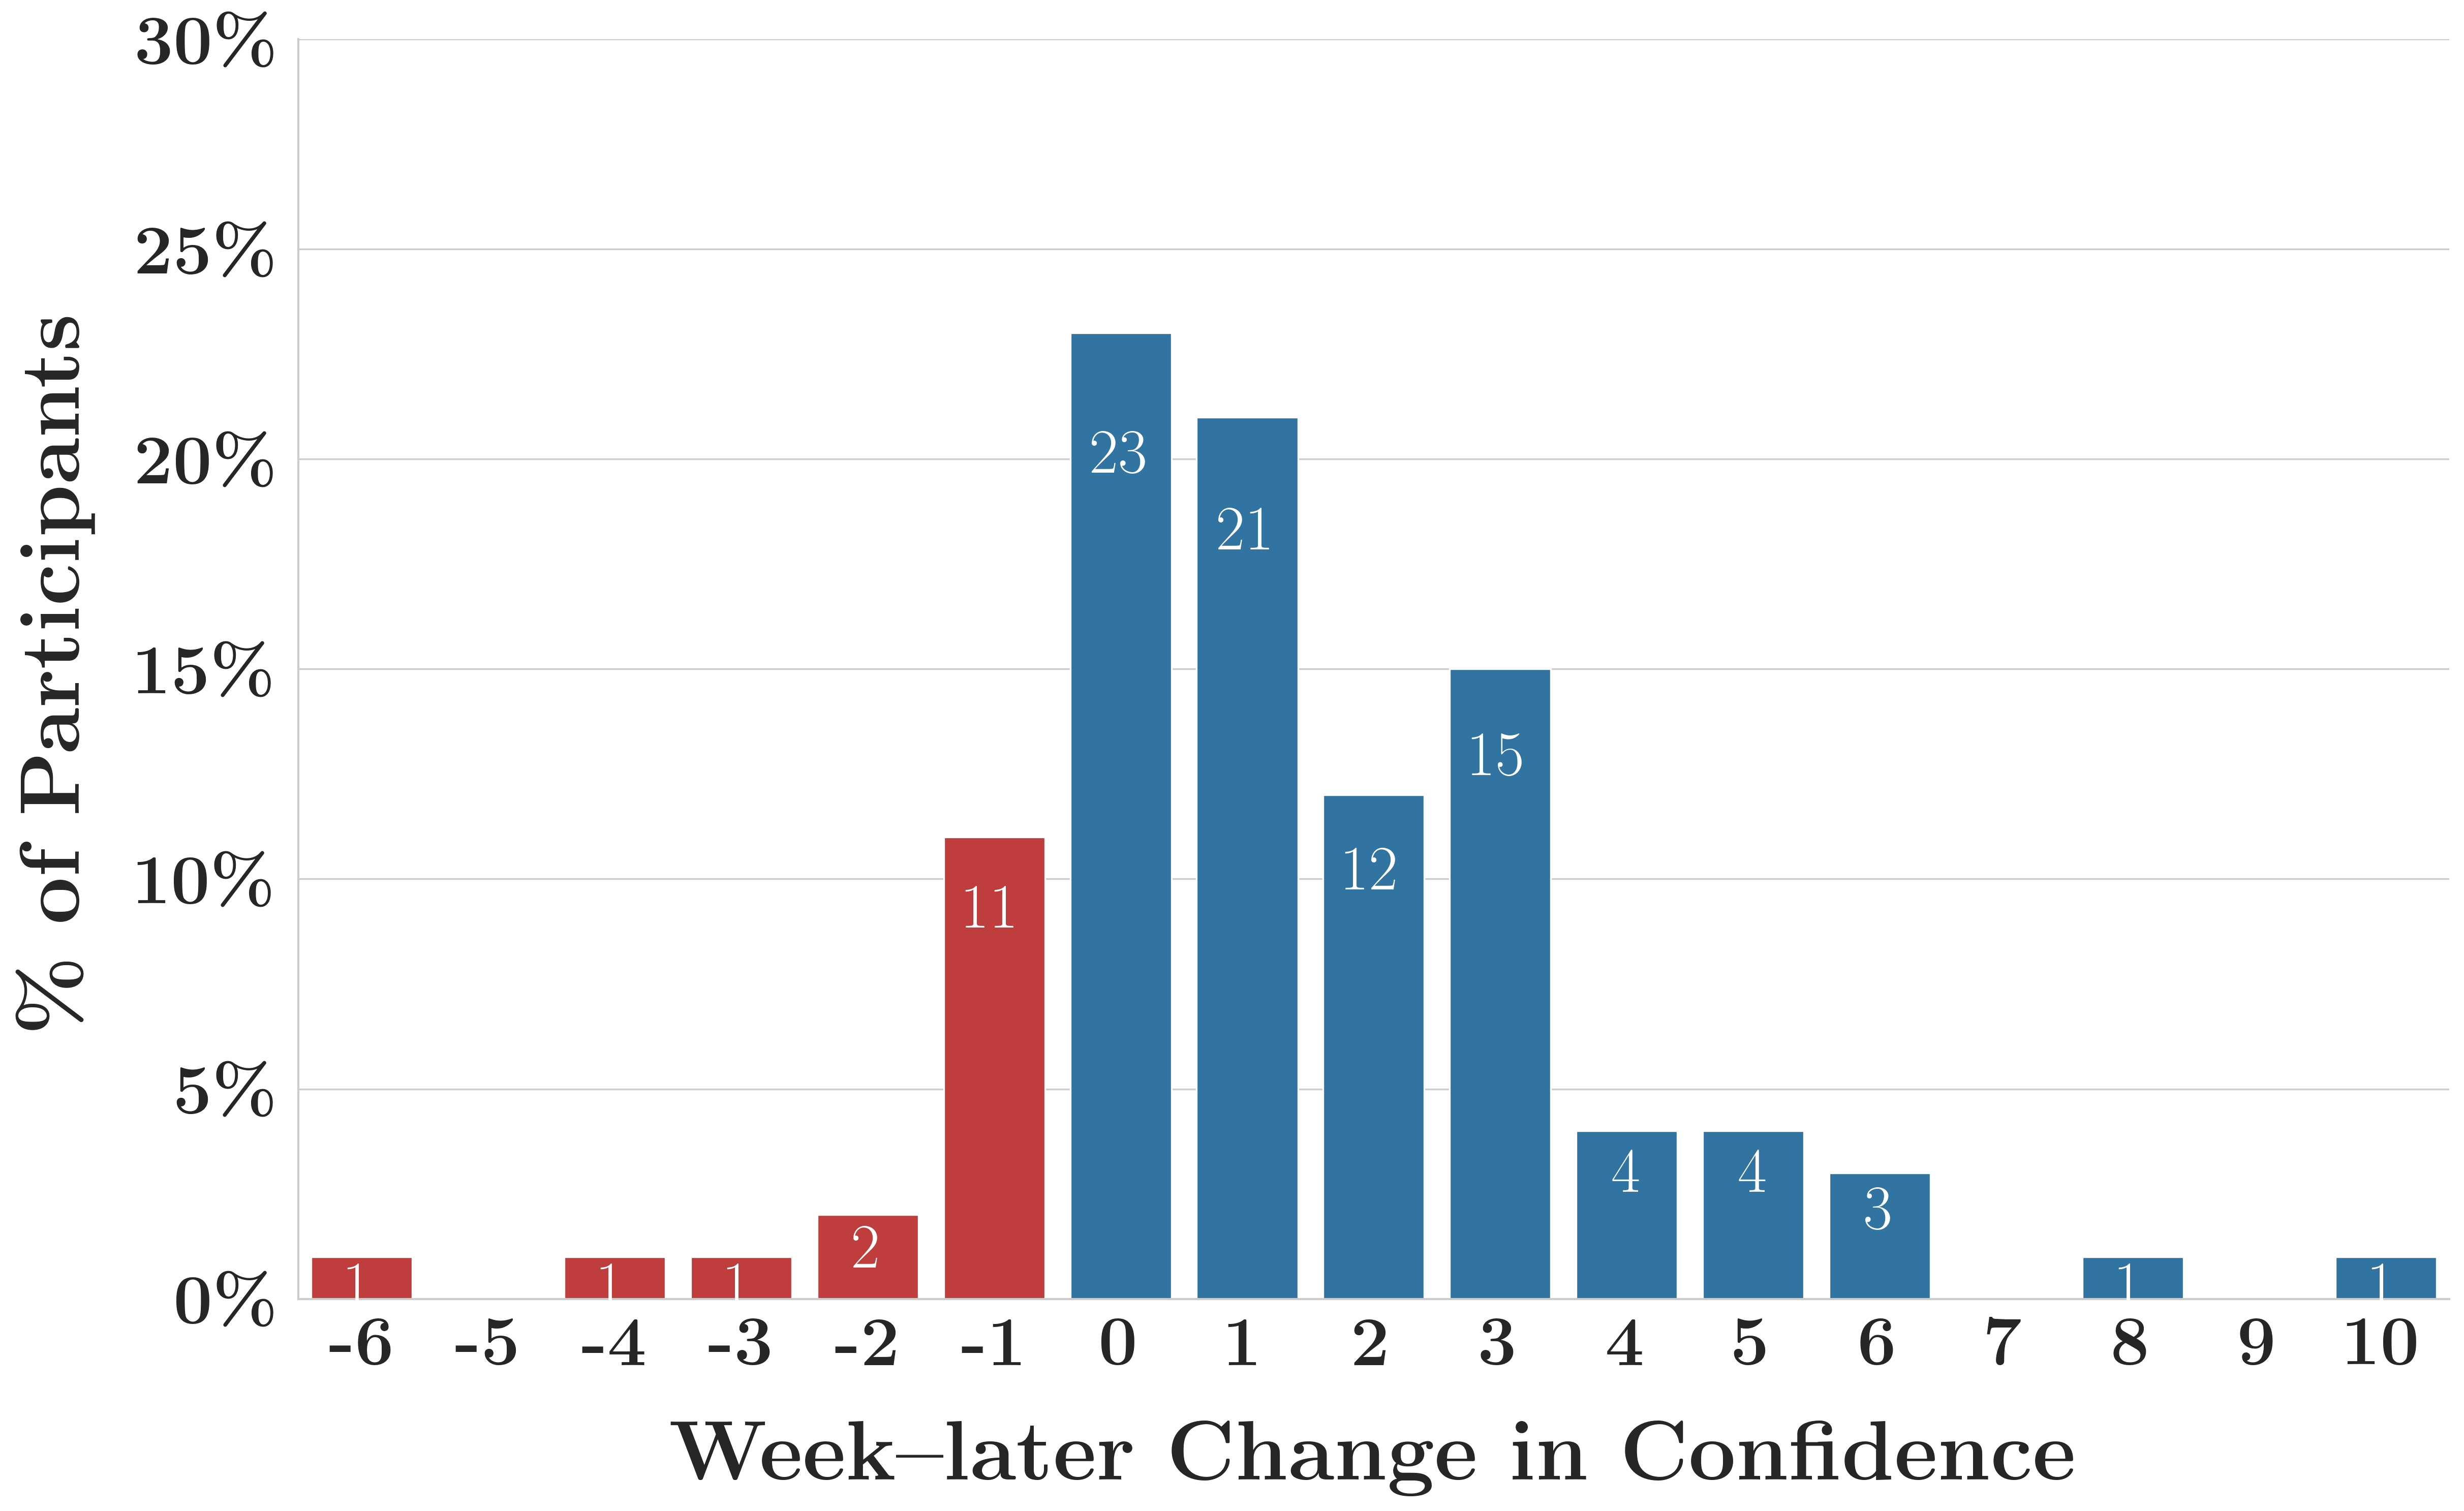
\includegraphics[width=\textwidth]{fig/MIV5.2_ruler_deltas_delta_with_week_later_keep_high_conf_False_change.png}
        \caption{MIBot v5.2}
        \label{fig:confidence_v5.2}
    \end{subfigure}
    \hfill
    \begin{subfigure}[b]{0.48\textwidth}
        \centering
        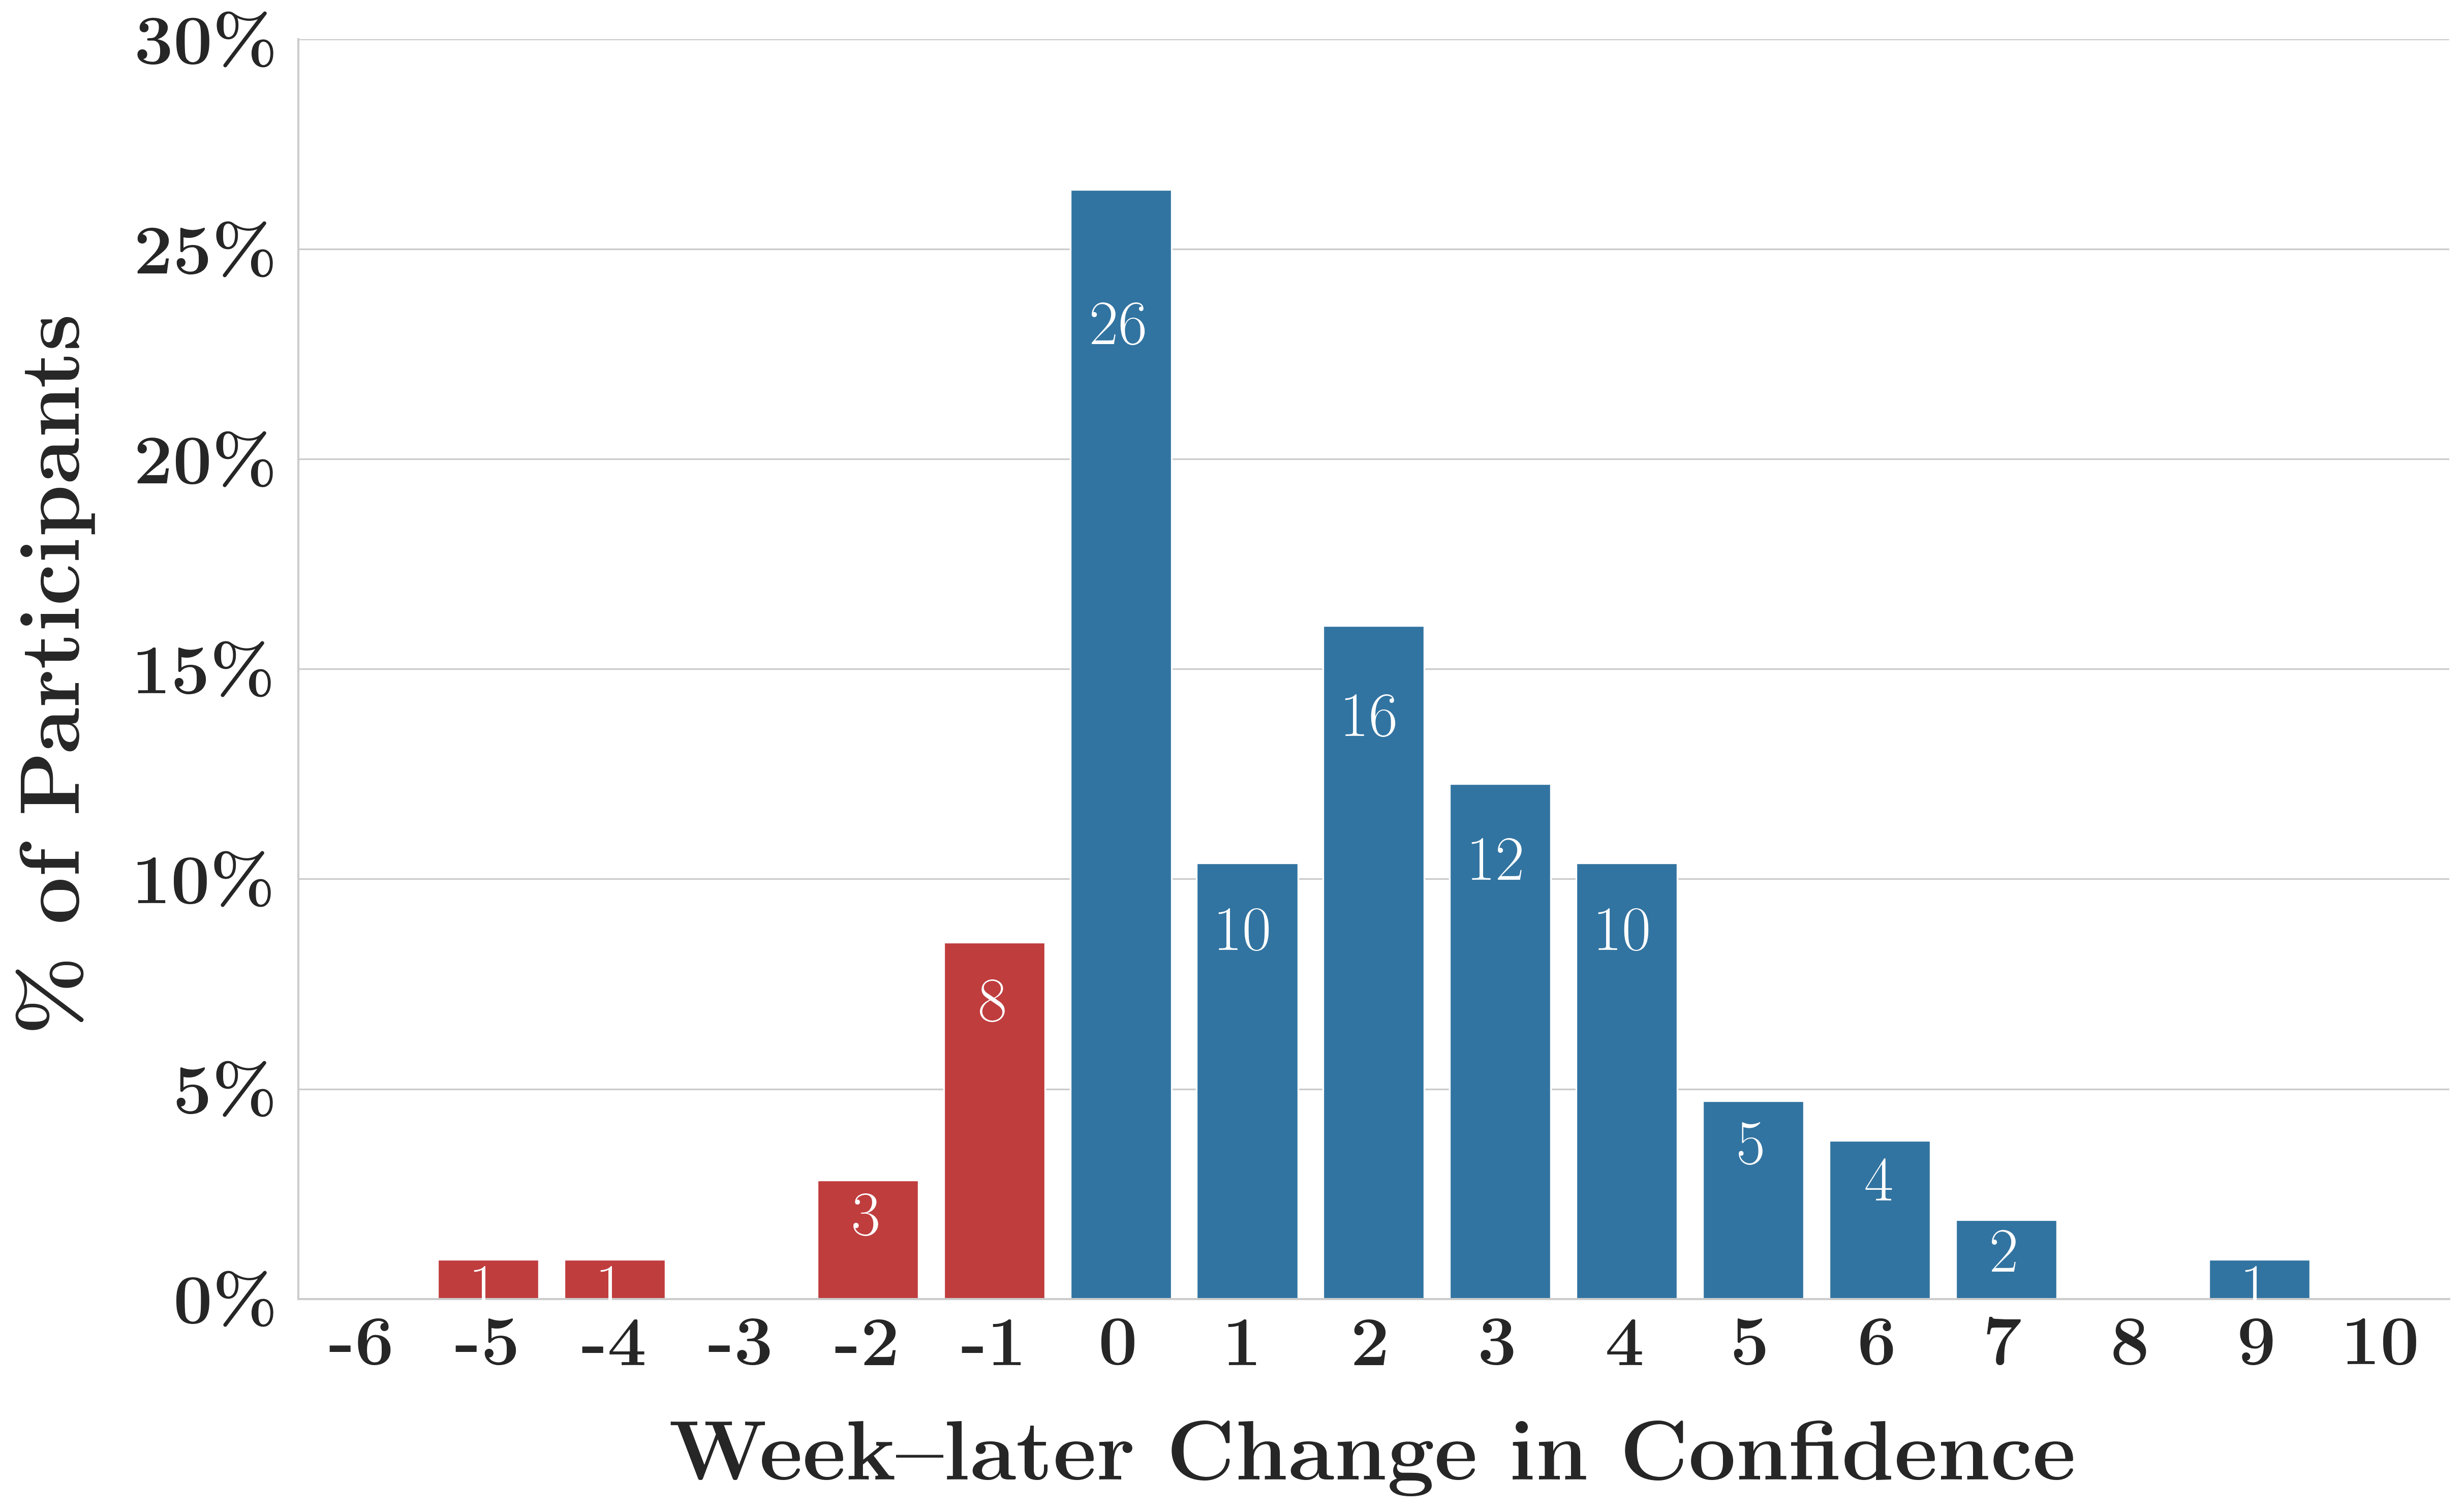
\includegraphics[width=\textwidth]{fig/2024-11-14-MIV6.3A-2024-11-22-MIV6.3A_ruler_deltas_delta_with_week_later_keep_high_conf_False_change.png}
        \caption{MIBot v6.3A}
        \label{fig:confidence_v6.3}
    \end{subfigure}

    
    \caption[Confidence Change Distributions for MIBot v5.2 and v6.3A]{Distribution of week-later confidence changes from baseline for MIBot v5.2 and MIBot v6.3A. The x-axis shows the change in confidence score, and the y-axis shows the number of participants. Red bars indicate a decrease in confidence, while blue bars indicate an increase or no change.}
    \label{fig:confidence_distributions}
\end{figure}










MIBot v5.2 achieved a mean confidence increase of 1.3 (SD 2.3, $p<0.001$) 
from baseline to one week later among 100 participants, and 
MIBot v6.3A achieved an increase of 1.7 (SD 2.4, $p<0.001$) among 106 participants.  
This difference was not statistically significant ($t(203.60) = 0.98$, 
$p = 0.165$, one-tailed, Cohen's $d = 0.14$). As shown in Figure~\ref{fig:confidence_distributions}, 
the distribution of confidence changes reveals interesting patterns: MIBot v6.3A 
resulted in more participants maintaining their baseline confidence (28\% vs.\ 23\% 
with no change) and fewer experiencing decreased confidence (13\% vs.\ 17\%).

For importance to quit, MIBot v5.2 achieved a significant increase of 0.7 (SD 2.0, $p<0.001$), while MIBot v6.3A showed a more modest but still significant gain of 0.5 (SD 1.7, $p<0.005$). Readiness changes were minimal and non-significant for both versions (v5.2: 0.4, SD 1.7, $p=0.01$; v6.3A: 0.3, SD 2.4, $p=0.22$).

\subsection*{Perceived Empathy Comparisons}

\begin{figure}[htbp]
    \centering
    \begin{subfigure}[b]{0.48\textwidth}
        \centering
        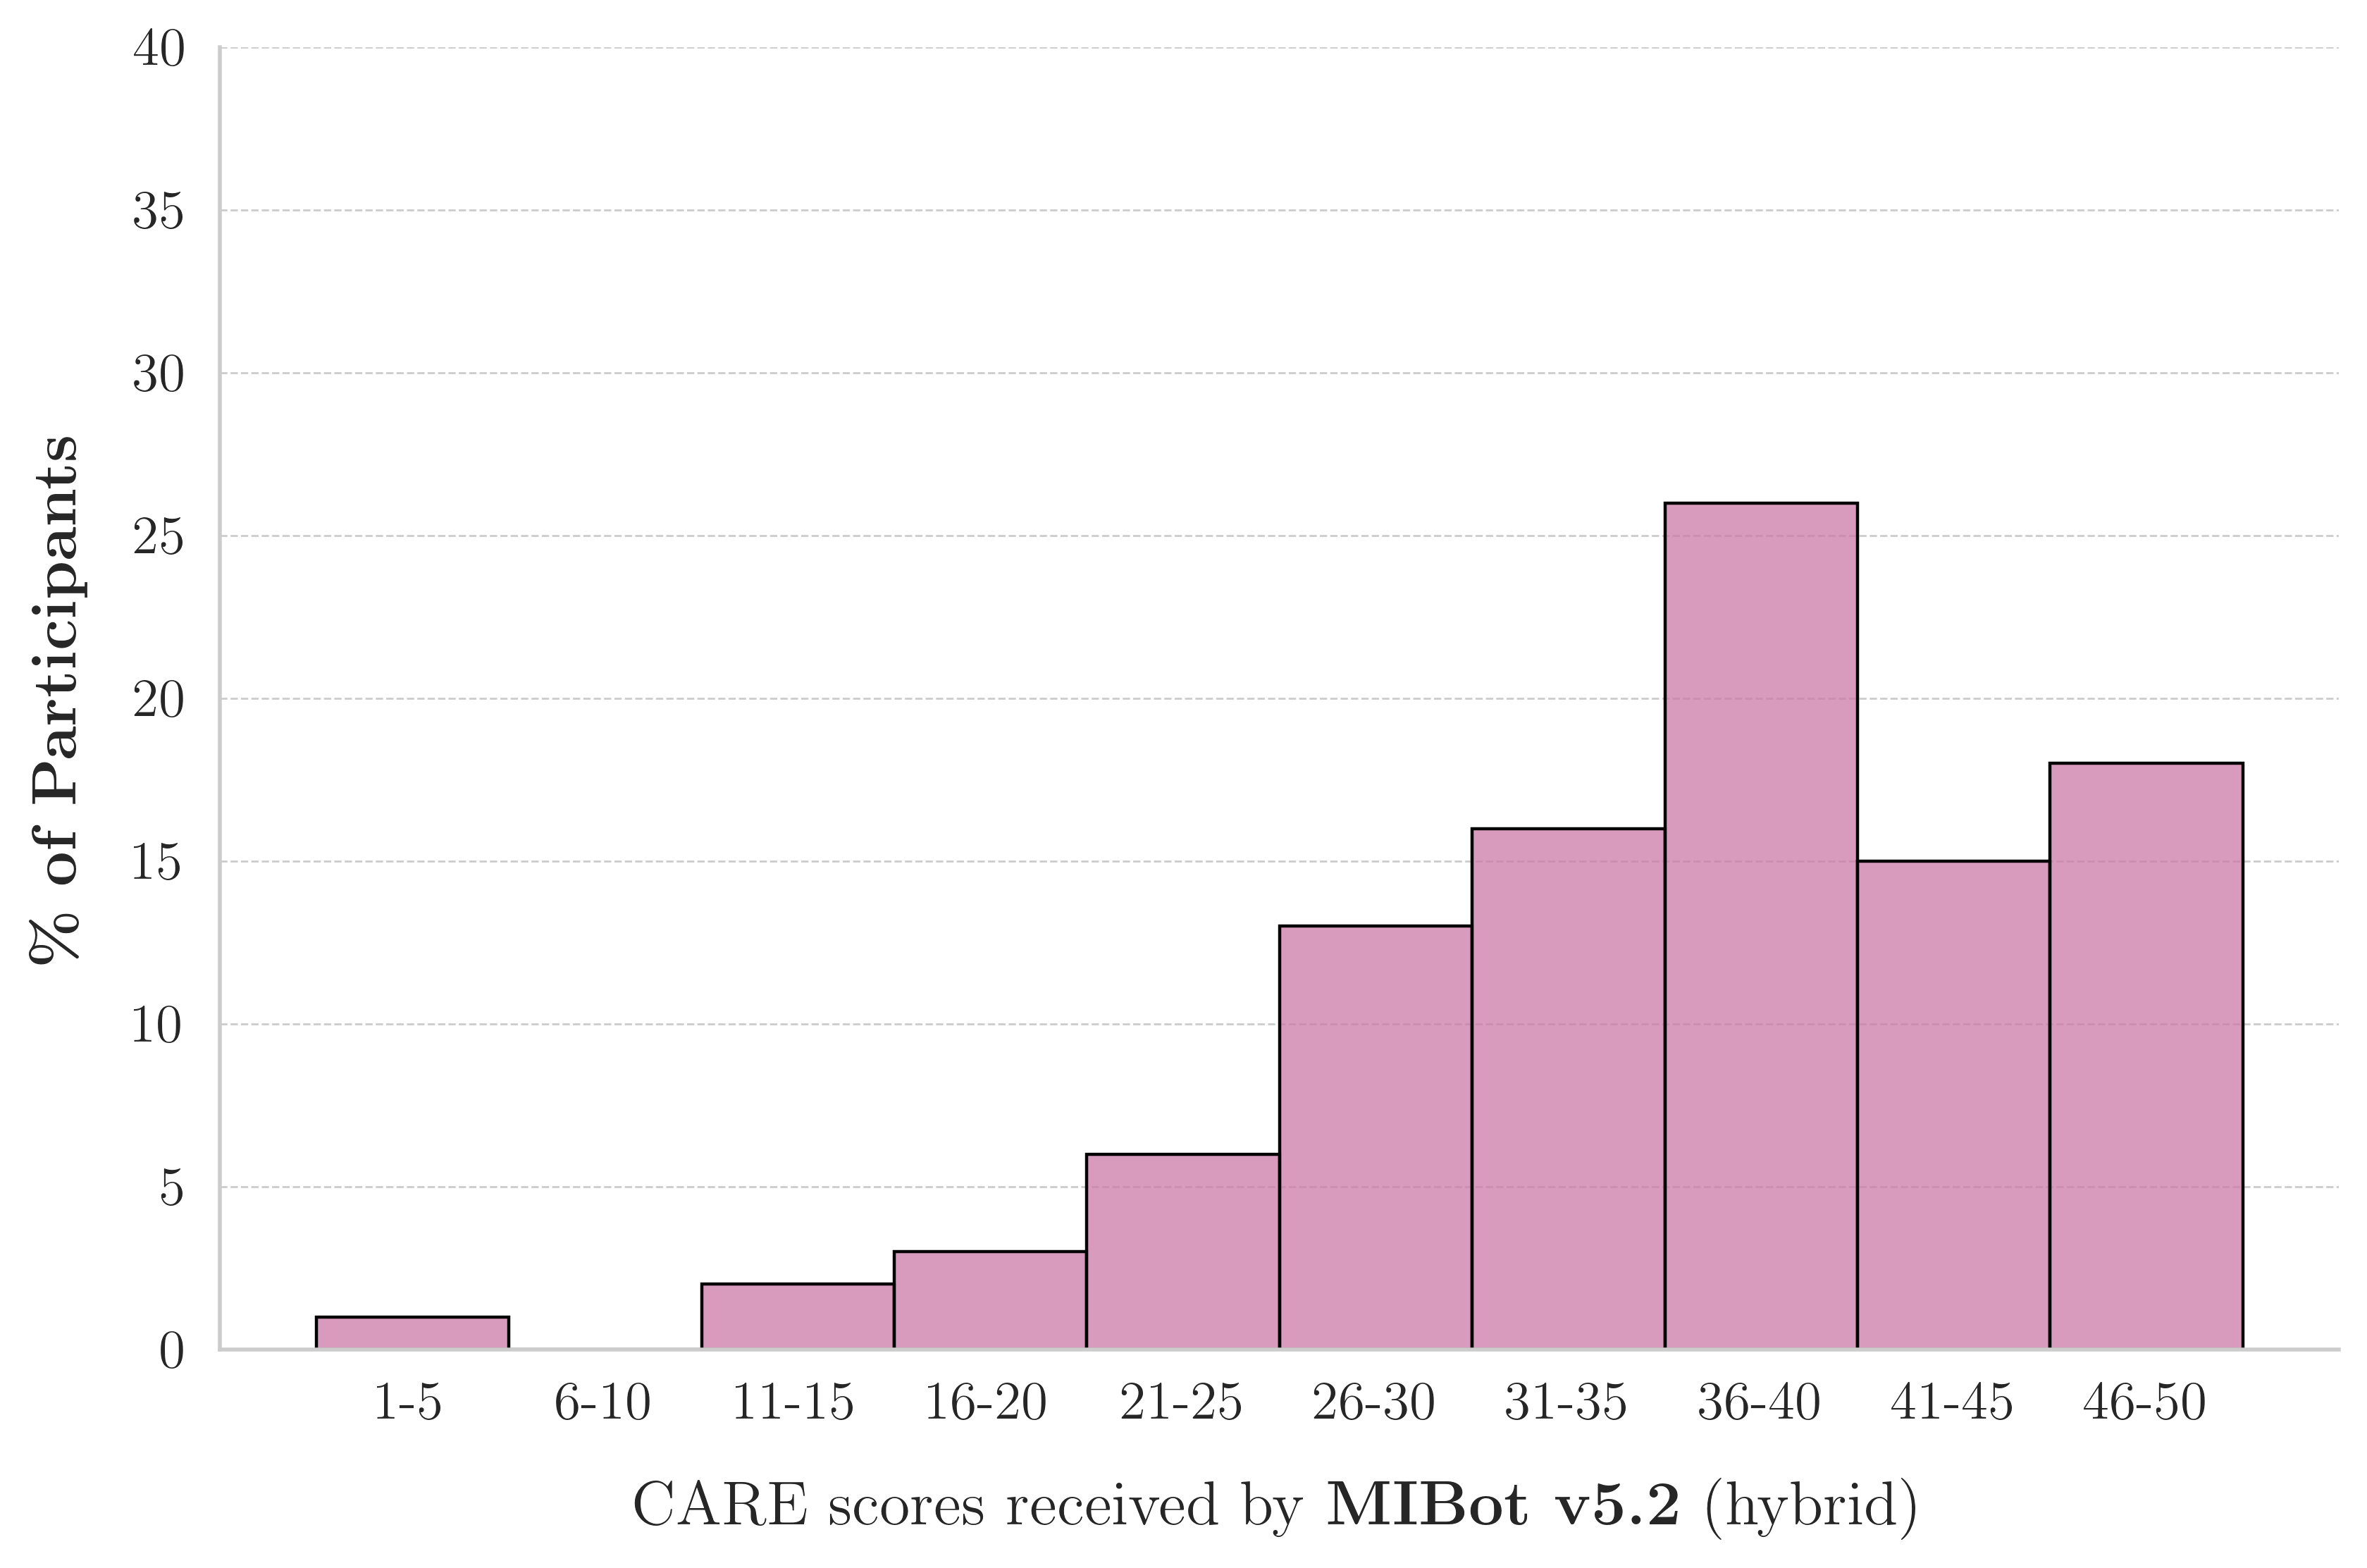
\includegraphics[width=\textwidth]{fig/MIV5.2_care_scores_histogram.png}
        \caption{MIBot v5.2 (hybrid)}
        \label{fig:care_v5.2}
    \end{subfigure}
    \hfill
    \begin{subfigure}[b]{0.48\textwidth}
        \centering
        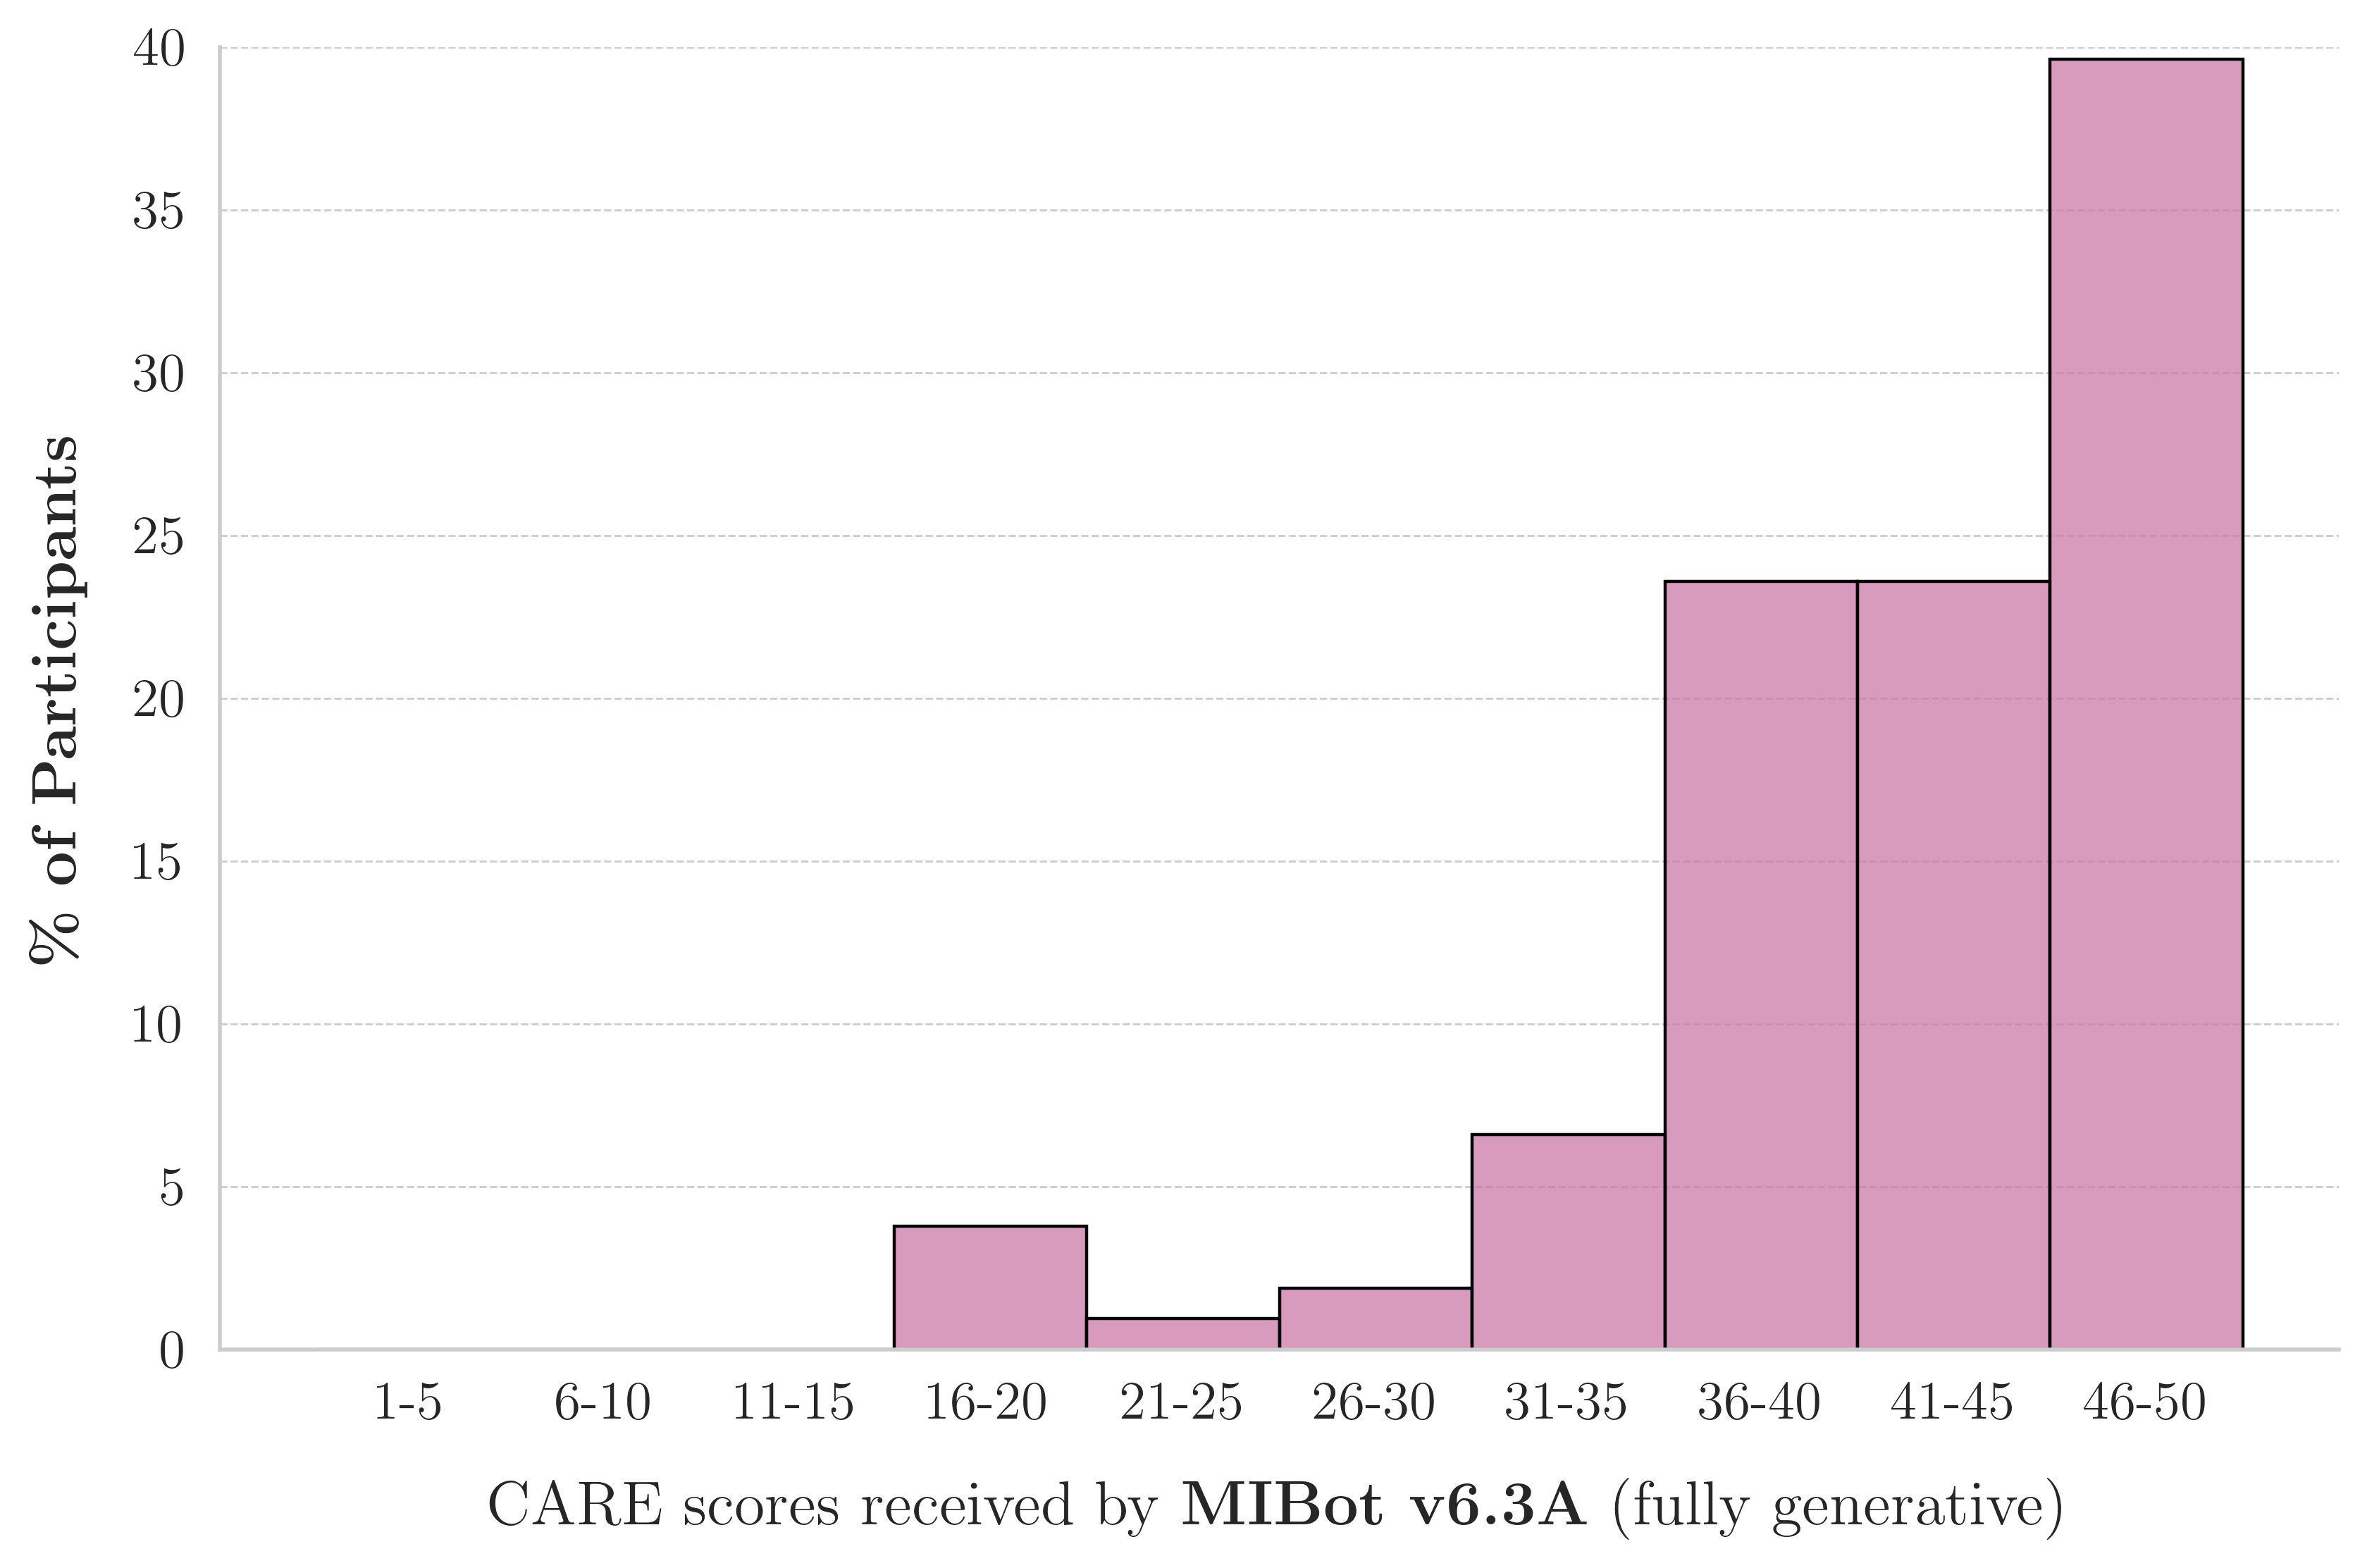
\includegraphics[width=\textwidth]{fig/2024-11-14-MIV6.3A-2024-11-22-MIV6.3A_care_scores_histogram.png}
        \caption{MIBot v6.3A (fully generative)}
        \label{fig:care_v6.3}
    \end{subfigure}
    \caption[CARE Score Distributions for MIBot v5.2 and v6.3A]{Distribution of CARE (Consultation and Relational Empathy) empathy scores for MIBot v5.2 and MIBot v6.3A. The x-axis represents the total CARE score, and the y-axis represents the number of participants. The distribution for the fully generative v6.3A is shifted to the right, indicating higher perceived empathy.}
    \label{fig:care_distributions}
\end{figure}

\begin{figure}[htbp]
    \centering
    \includegraphics[width=0.98\textwidth]{fig/combined_care_scores_with_improvement.png}
    \caption[Comparison of Mean CARE Scores per Question]{Comparison of mean CARE (Consultation and Relational Empathy) scores for each question between MIBot v5.2 (hybrid) and v6.3A (fully generative). The x-axis lists the 10 CARE questions, and the y-axis shows the mean score. The fully generative version shows improvement across all dimensions.}
    \label{fig:care_questions}
\end{figure}

 MIBot v5.2 achieved a mean CARE score of 36 (SD = 9.1), with only 3\% of participants awarding a perfect score, while MIBot v6.3A achieved a mean score of 42 (SD = 7.5), with 11\% receiving perfect scores. This difference was statistically significant ($t(191.67) = 4.96$, $p < .001$, Cohen's $d = 0.70$), representing a medium-to-large effect size, and suggests that the fully generative responses of v6.3A significantly improved perceived empathy. Figure~\ref{fig:care_distributions} illustrates the distributional shift between versions. The hybrid v5.2 shows a relatively normal distribution centred in the mid-30s, with considerable spread across all score ranges, whereas v6.3A demonstrates a clear rightward skew, with 40\% of participants rating the chatbot in the highest range (46--50).

To understand which aspects of empathetic interaction improved most, Figure~\ref{fig:care_questions} presents the mean scores across all ten CARE dimensions. The fully generative approach exhibits improvements across every dimension, with particularly notable gains in emotional and communicative aspects. The largest relative improvement was observed in ``showing care and compassion'' (+32\%), reflecting the chatbot's enhanced ability to maintain an encouraging tone. Interestingly, the dimension of ``making a plan of action with you'' remained the weakest aspect for both versions (2.73 for v5.2, 3.59 for v6.3A), despite showing considerable relative improvement (+32\%). It is worth noting that MIBot v6.3 was prompted with detailed guidelines on how to make a plan of action with the client. Despite this, planning seems to be one of its weak areas.



\subsection*{Implications of the Comparison}

The fully generative MIBot v6.3A chatbot scored higher on CARE, the measure of perceived therapeutic alliance. This improvement suggests that participants experienced more authentic, personalized interactions when the entire conversation---not just reflections---emerged from the language model's contextual understanding. However, both chatbots scored similarly on our primary metric of effectiveness, viz. the week-later change in confidence, indicating that the core therapeutic mechanism of MI may be responsible for most of the gains in confidence. This finding aligns with prior work showing that even simple question-asking can produce substantial benefits \citep{brown2023mi}, though the enhanced empathy of full generation may improve engagement and retention in real-world deployment.

\section{AutoMISC Analysis}
\label{sec:mi-adherence}

To evaluate the chatbot's adherence to MI principles, we analysed counsellor and client utterances from the feasibility study transcripts (\cref{ch:feasibility}) using AutoMISC, an automated annotation system originally described in \citet{mahmood-etal-2025-fully}\footnote{A comprehensive description of the AutoMISC system by \citet{ali2025automated} is forthcoming}.
The system assigns behavioural codes to each utterance: counsellor utterances are classified as MI-Consistent (MICO), MI-Inconsistent (MIIN), Reflection (R), Question (Q), or Other (O), while client utterances are categorized as change talk (C), sustain talk (S), or neutral (N). Following annotation of all utterances, we computed per-transcript summary metrics to quantify MI adherence. These comprise:

\begin{itemize}

    \item \textbf{Percentage MI-Consistent Responses (\%MIC):} The proportion of counsellor utterances that align with MI principles. Higher values indicate greater adherence to MI methodology.
    
    \item \textbf{Reflection-to-Question Ratio (R:Q):} The ratio of counsellor utterances labelled as reflection (R) to those labelled as question (Q). This metric assesses the balance between reflective listening and questioning. Values between 1 and 2 are considered indicative of proficiency \citep{moyers2016miti}.

    \item \textbf{Percentage Change Talk (\%CT):} The proportion of client utterances expressing motivation toward behaviour change. Higher values are associated with improved behavioural outcomes \citep{Apodaca2009}.

\end{itemize}

\subsection{Contextualizing AutoMISC Metrics With the HLQC Dataset}
To provide a point of comparison for the MISC summary metrics, we also ran AutoMISC on the HighLowQualityCounselling (HLQC) dataset  \cite{perez-rosas-etal-2019-makes}, a publicly available\footnote{ \url{https://lit.eecs.umich.edu/downloads.html}} corpus of transcribed MI counselling demonstrations. The HLQC dataset comprises 155 high-quality (HLQC\_\textbf{HI}) and 104 low-quality (HLQC\_\textbf{LO}) transcripts sourced from public websites.
We computed summary scores separately for these subsets and then compared MIBot's summary metrics against those of both HLQC\_HI and HLQC\_LO.

\subsection{Counsellor Behaviour Metrics}
\begin{table}[ht]
  \centering
  \small
  \setlength{\tabcolsep}{4pt}
  \renewcommand{\arraystretch}{1.1}
  \begin{tabular}{@{}lcc@{}}
    \toprule
    \textbf{Metric} & \textbf{MIBot} & \textbf{HLQC\_HI (high-quality)} \\
    \midrule
    \%MI-consistent (\%MIC) & 98 (3.6) & 92 (9.8) \\
    Reflection-to-Question Ratio (R:Q) & 1.3 (0.3) & 2.3 (5.7) \\
    \bottomrule
  \end{tabular}
  \caption[AutoMISC Counsellor Metrics for MIBot vs. Human]{Counsellor-specific summary metrics from AutoMISC for MIBot, compared to high-quality human counselling sessions from the HLQC dataset. The table shows the mean (and standard deviation) for the percentage of MI-consistent responses (\%MIC) and the reflection-to-question ratio (R:Q).}
  \label{table:automisc_summary}
\end{table}

Figure~\ref{fig:misc_distributions} shows violin plots comparing the distribution of \%MIC, R:Q, and \%CT across MIBot conversations with the HLQC benchmarks. The \%MIC scores are tightly clustered near 100\%, with only a few transcripts falling below 80\%. The R:Q distribution is centred around 1.3, showing less variance than human counsellors who range from pure question-asking (R:Q near 0) to heavy reflection use (R:Q $>$ 5).

\begin{figure}[htpb]
\centering
\begin{subfigure}[b]{0.9\textwidth}
\centering
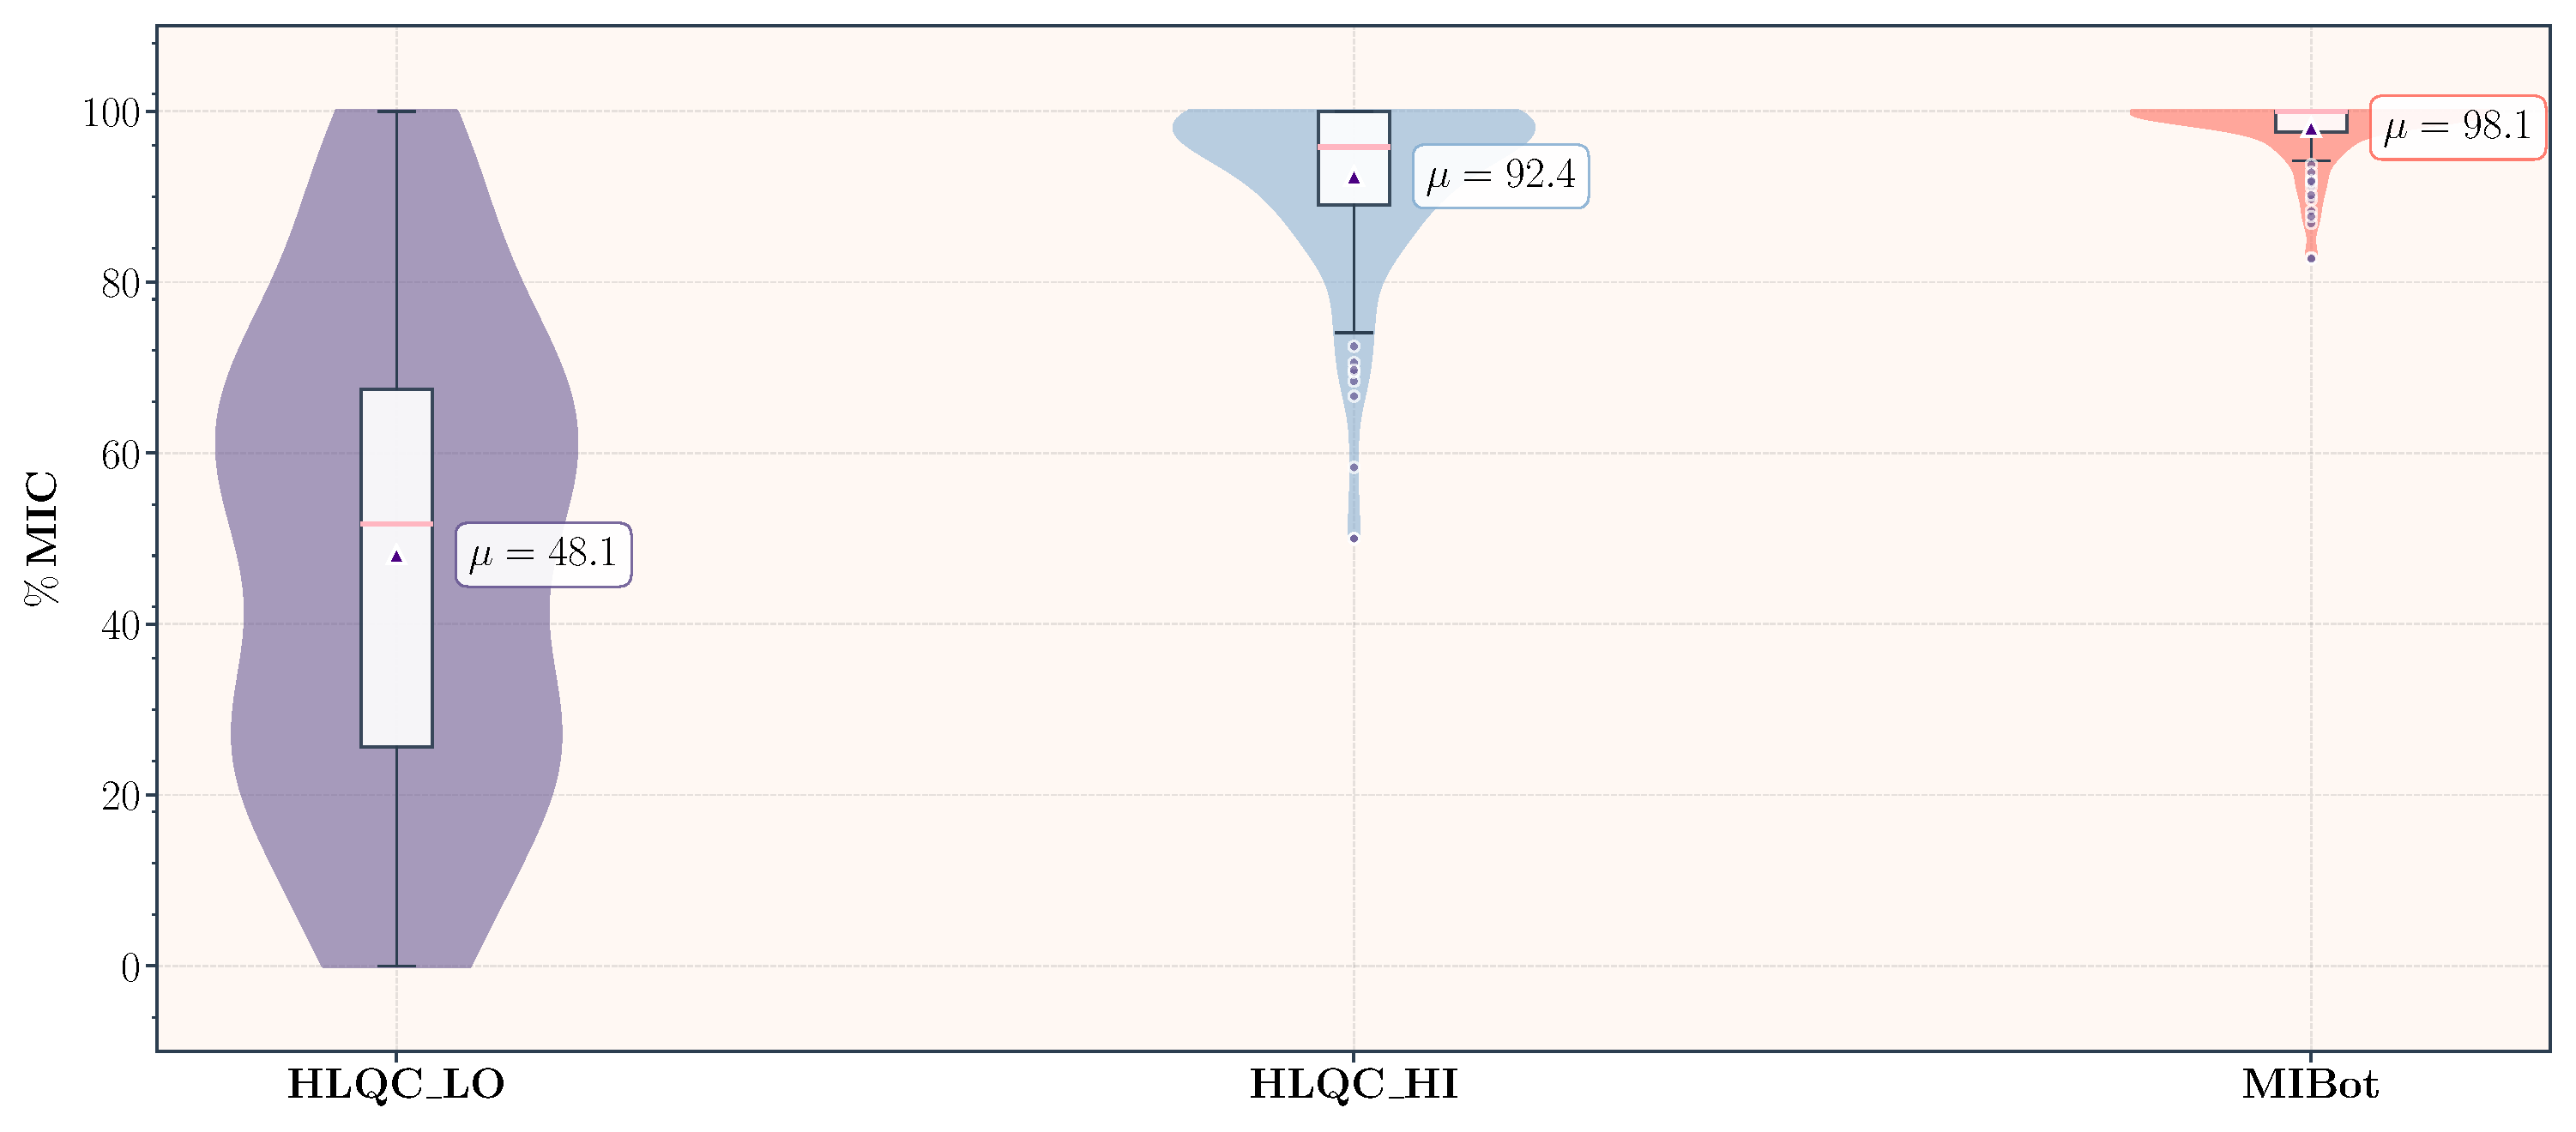
\includegraphics[height=0.25\textheight, keepaspectratio]{fig/mic_enhanced.pdf}
\caption{\%MIC}
\end{subfigure}

\begin{subfigure}[b]{0.9\textwidth}
\centering
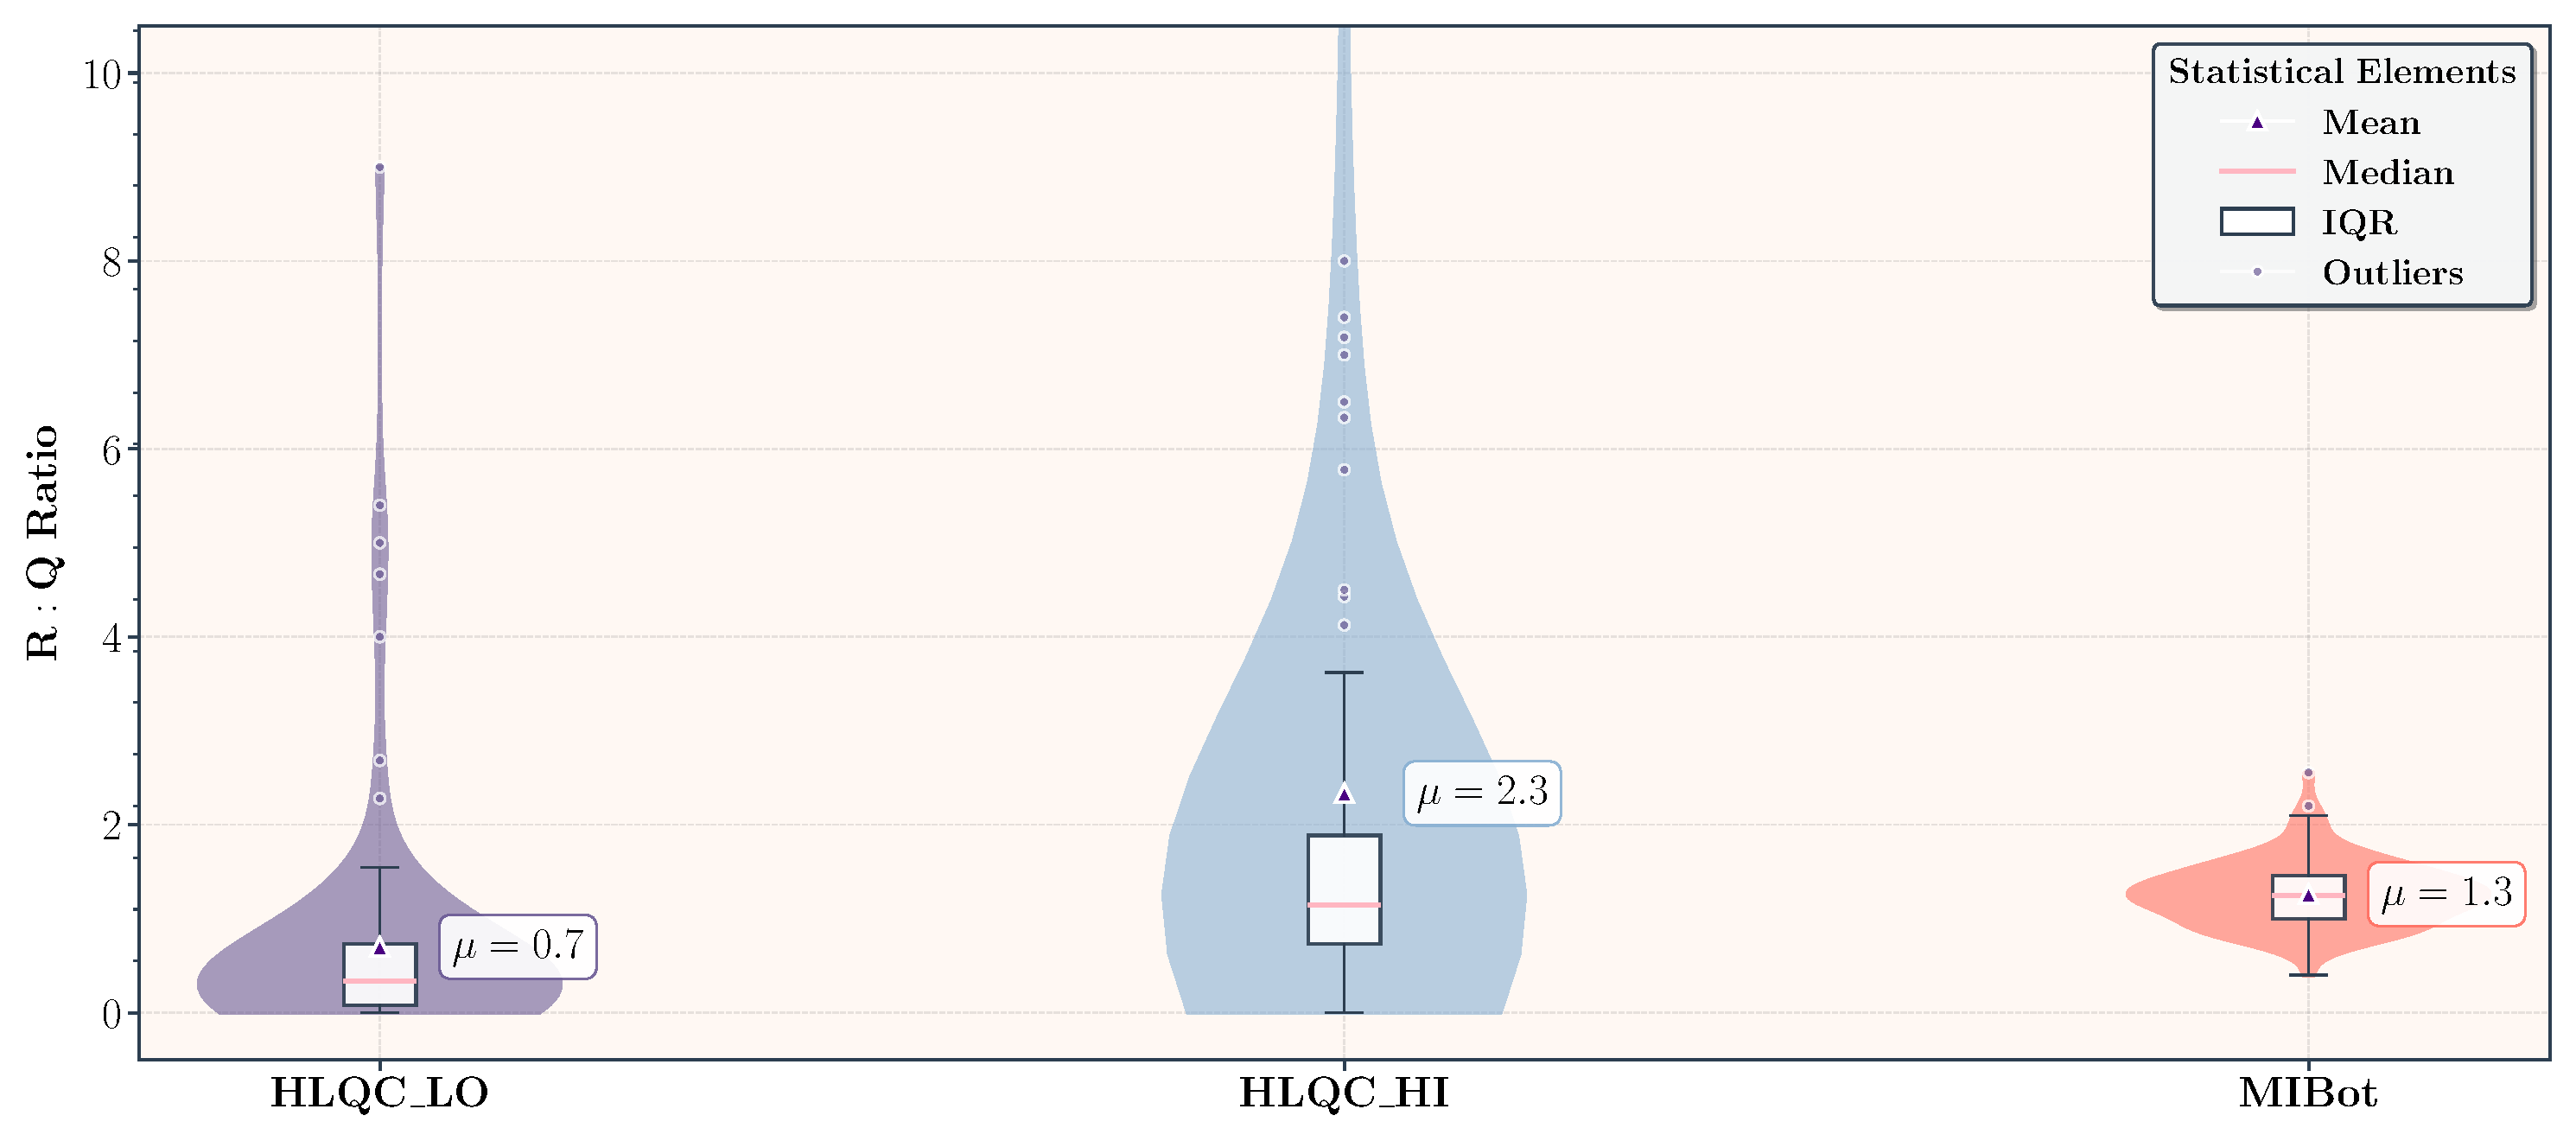
\includegraphics[height=0.25\textheight, keepaspectratio]{fig/rq_enhanced.pdf}
\caption{R:Q}
\end{subfigure}

\begin{subfigure}[b]{0.9\textwidth}
\centering
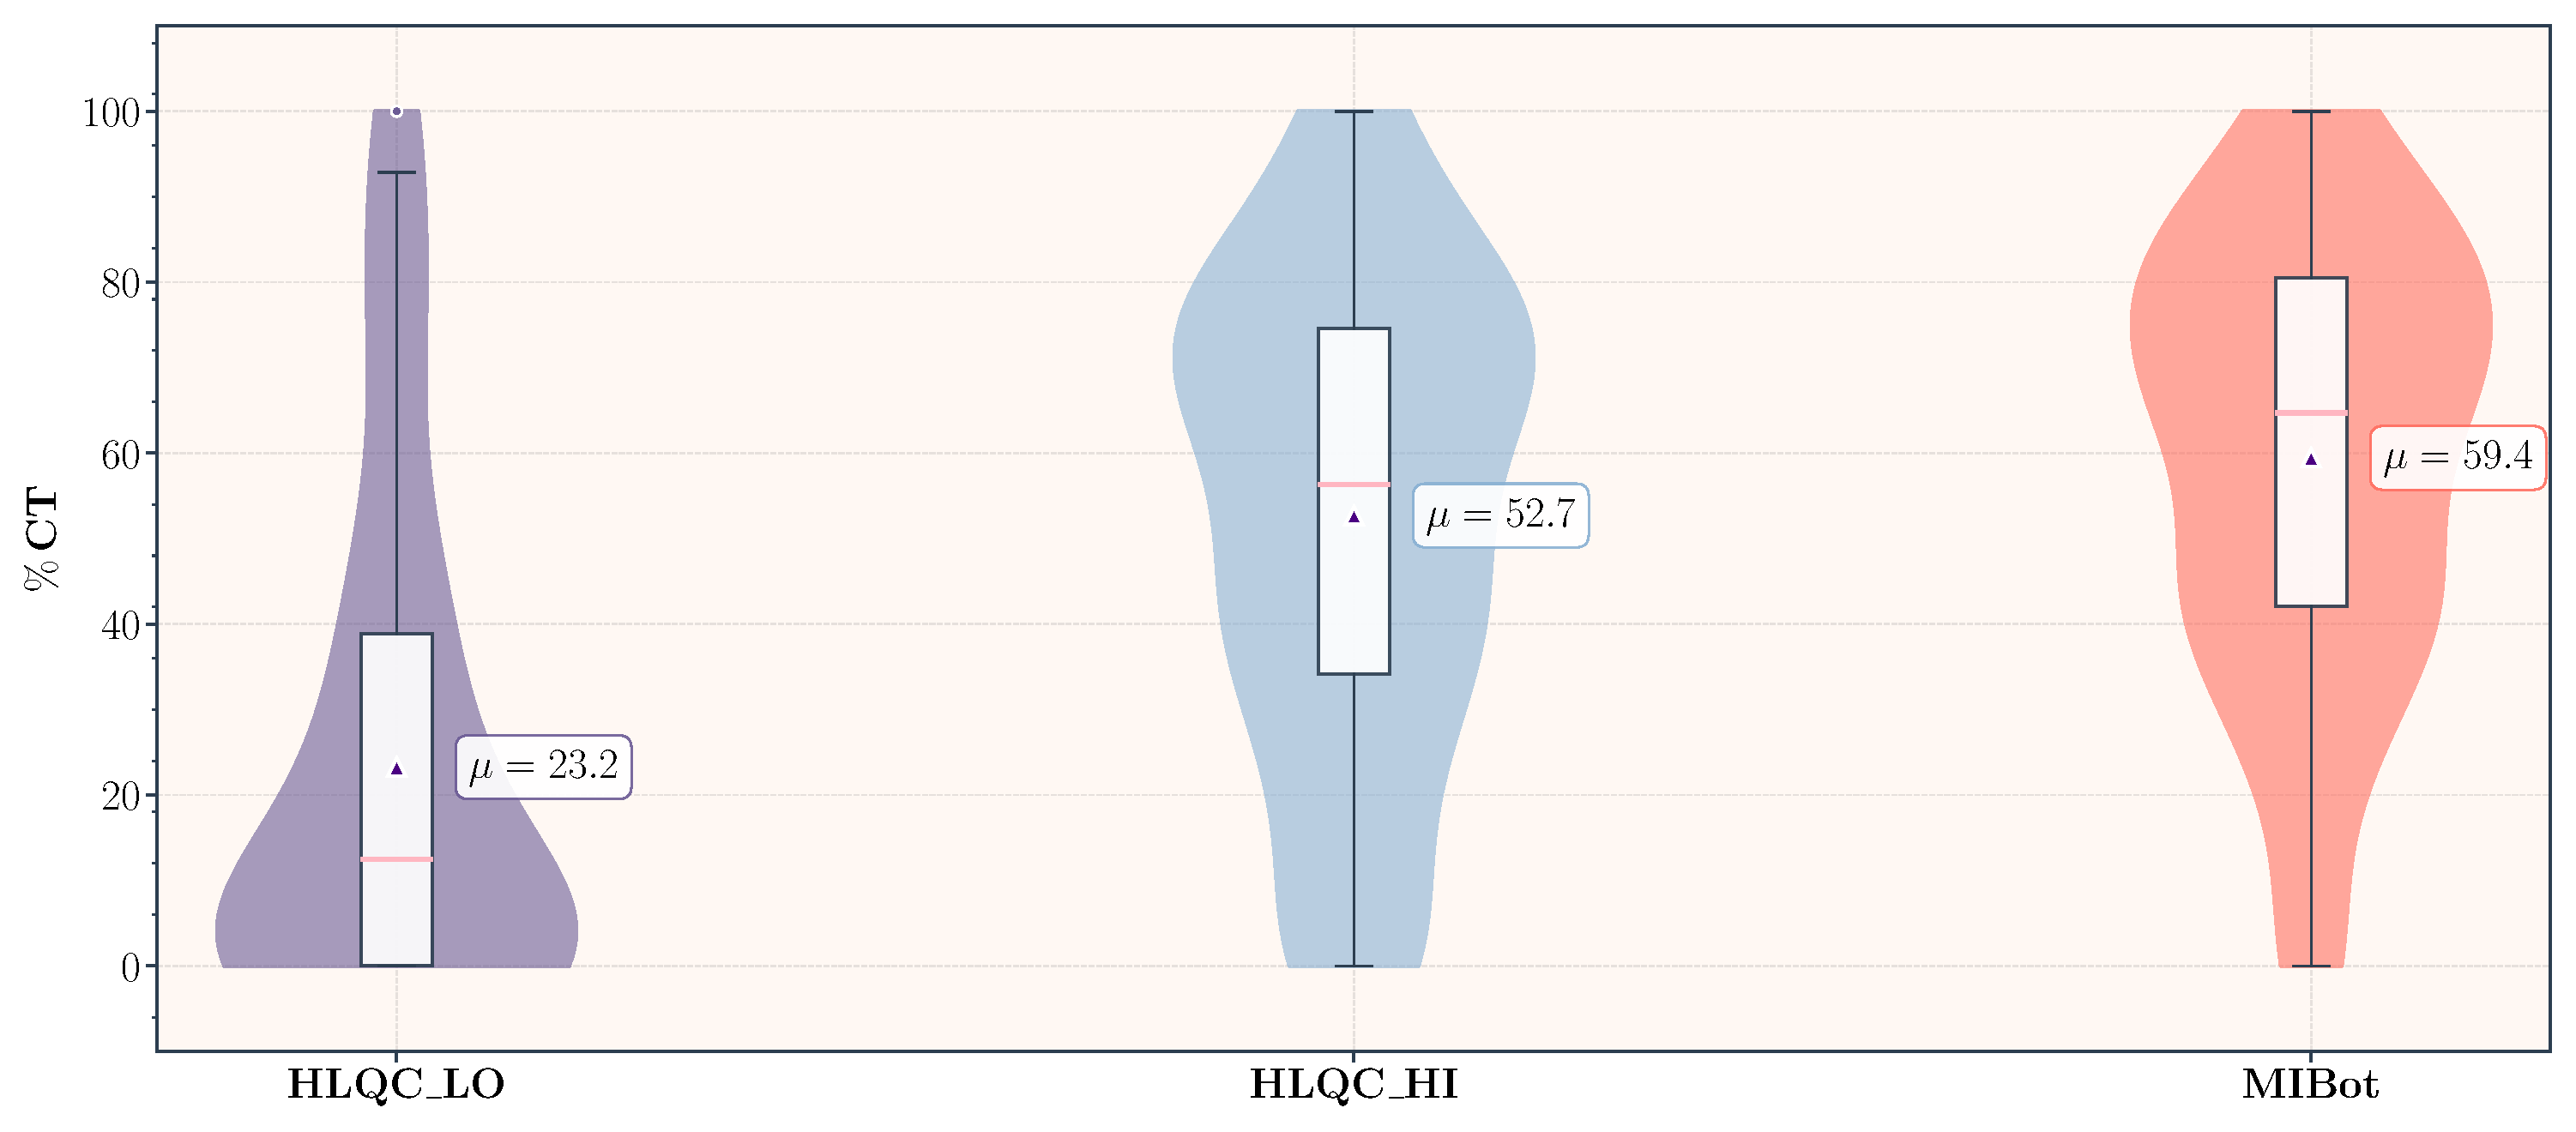
\includegraphics[height=0.25\textheight, keepaspectratio]{fig/cs_enhanced.pdf}
\caption{\%CT}
\end{subfigure}

\caption[Comparison of MISC summary score distributions for MIBot and the HLQC dataset.]{Comparison of MISC summary score distributions for MIBot and the HLQC dataset (high and low quality). The figure shows violin plots for (a) Percentage MI-Consistent Responses (\%MIC), (b) Reflection to Question Ratio (R:Q), and (c) Percentage Client Change Talk (\%CT). Taken from \citet{ali2025thesis}}.
\label{fig:misc_distributions}
\end{figure}


\subsection{Client Change Talk Analysis}



\begin{table}[ht]
  \centering
  \small
  \setlength{\tabcolsep}{4pt}
  \renewcommand{\arraystretch}{1.1}
  \begin{tabular}{@{}lcc@{}}
    \toprule
    \textbf{Metric} & \textbf{MIBot} & \textbf{HLQC\_HI (high-quality)} \\
    \midrule
    \%Change Talk (\%CT) & 59 (29.6) & 53 (28.54) \\
    \bottomrule
  \end{tabular}
  \caption[AutoMISC Client Metrics for MIBot vs. Human]{Client-specific summary metric from AutoMISC for MIBot, compared to high-quality human counselling sessions from the HLQC dataset. The table shows the mean (and standard deviation) for the percentage of change talk (\%CT).}
  \label{table:automisc_summary_client}
\end{table}


Figure~\ref{fig:misc_distributions}(c) illustrates the distribution of \%CT across conversations. Most sessions by MIBot had a \%CT of $>$ 60\%, and the distribution closely matches that of the \textbf{HLQC\_HI} dataset. Overall, the mean \%CT was 59\% for MIBot, compared to 53\% for the \textbf{HLQC\_HI} dataset.


%%%%%%%%%%%%%%%%%%%%%%%%%%%%%%%%%%%%%%%%%%%%%%%%

% WIP Below

% Please edit it later!


%%%%%%%%%%%%%%%%%%%%%%%%%%%%%%%%%%%%%%%%%%%%%%%%%




























\section{Behavioural Outcomes}


\label{sec:behavioural-outcomes}

\subsection*{Quit Attempts at One Week}

\begin{table}[ht]
  \centering
  \small
  \setlength{\tabcolsep}{4pt}
  \renewcommand{\arraystretch}{1.1}
  \begin{tabular}{@{}lcc@{}}
    \toprule
    \textbf{Quit Attempt Status} & \textbf{Pre-conversation} & \textbf{Post-conversation} \\
    \midrule
    Made attempt & 34 (32.1\%) & 37 (34.9\%) \\
    No attempt & 72 (67.9\%) & 69 (65.1\%) \\
    \midrule
    New attempters & -- & 15 (14.2\%) \\
    Sustained attempters & -- & 22 (20.8\%) \\
    \bottomrule
  \end{tabular}
  \caption[Quit Attempt Behaviour Before and After MIBot]{Summary of participants' quit attempt behaviour before and after the MIBot conversation. The table shows the number and percentage of participants who made a quit attempt in the week prior to the conversation and in the week following the conversation.}
  \label{table:quit_attempts}
\end{table}

Participants who made quit attempts post-conversation showed larger confidence gains (mean +2.43) compared to those who did not attempt (+1.35, $p<0.05$). This bidirectional relationship---where confidence predicts attempts and attempts reinforce confidence---aligns with social cognitive theory \citep{Bandura1986}.

\subsection*{Self-Reported Behavioural Changes}

Beyond formal quit attempts, participants reported various harm reduction behaviours. Analysis of open-ended responses revealed five main categories of behavioural change:

\begin{enumerate}
\item \textbf{Reduced consumption} (42\% of participants): ``Cut down from 20 to 12 cigarettes a day.''
\item \textbf{Delayed first cigarette} (28\%): ``Now waiting until after breakfast instead of immediately upon waking.''
\item \textbf{Substitution strategies} (31\%): ``Using nicotine gum when cravings hit at work.''
\item \textbf{Environmental changes} (19\%): ``Removed ashtrays from the house and car.''
\item \textbf{Social support seeking} (23\%): ``Told my partner about wanting to quit and asked for support.''
\end{enumerate}

These incremental changes, while not constituting complete cessation, represent important steps in the behaviour change process and align with harm reduction approaches increasingly recognized in tobacco control \citep{Abrams2018}.

\section{Conversation Analysis}
\label{sec:conversation-analysis}

\subsection*{Quantitative Dynamics}
\label{sec:conversation-dynamics}

Conversations ranged from 36 to 163 utterances (median 78; mean 80.7, SD 29.4), with counsellor utterances comprising 55\% of the total. The median conversation lasted approximately 19 minutes based on participant self-report. Table~\ref{table:conversation_metrics} summarizes key quantitative metrics.

\begin{table}[ht]
  \centering
  \small
  \setlength{\tabcolsep}{4pt}
  \renewcommand{\arraystretch}{1.1}
  \begin{tabular}{@{}lcc@{}}
    \toprule
    \textbf{Metric} & \textbf{Mean (SD)} & \textbf{Range} \\
    \midrule
    Total utterances & 80.7 (29.4) & 36--163 \\
    Counsellor utterances & 44.4 (16.2) & 20--90 \\
    Client utterances & 36.3 (13.2) & 16--73 \\
    Words per counsellor utterance & 42.3 (18.7) & 15--95 \\
    Words per client utterance & 28.6 (15.4) & 8--72 \\
    Session duration (minutes) & 19 (9) & 8--45 \\
    \bottomrule
  \end{tabular}
  \caption[Conversation Dynamics between Participants and MIBot: Quantitative Metrics]{Quantitative metrics of the conversation dynamics between participants and MIBot. The table includes statistics on the total number of utterances, counsellor and client utterances, words per utterance, and session duration.}
  \label{table:conversation_metrics}
\end{table}

Longer conversations correlated with better outcomes ($r=0.20$ for confidence change), but the relationship was non-linear. Conversations under 50 utterances rarely produced substantial gains, while those exceeding 120 utterances showed diminishing returns, suggesting an optimal engagement window of 60--100 exchanges.

\subsection*{Qualitative Thematic Analysis}

To understand the qualitative aspects of the conversations, a thematic analysis was performed on the full corpus of transcripts. The analysis was conducted by two researchers who independently reviewed the transcripts to identify recurring patterns and themes. They then met to compare their findings, discuss discrepancies, and collaboratively develop a final set of themes that characterized successful therapeutic engagement. This process revealed four recurring patterns:

\subsubsection*{Stress and Coping Narratives}

The most common theme (78\% of conversations) involved smoking as emotional regulation. Participants frequently described smoking as their primary stress management tool:

\begin{quote}
\textit{``It's like my safety blanket. When work gets overwhelming, that cigarette break is the only thing that keeps me sane. I know it's killing me, but it's also what's keeping me functional right now.''}
\end{quote}

In these situations, the chatbot's responses often involved reflective listening to validate users' feelings before exploring alternatives, a pattern consistent with the double-sided reflection technique in MI.

\subsubsection*{Social and Ritualistic Aspects}

Many participants (62\%) described smoking as deeply embedded in social routines and relationships:

\begin{quote}
\textit{``All my friends smoke. Our whole social life revolves around smoke breaks at work, cigarettes with coffee, smoking outside the pub. If I quit, I lose all that connection.''}
\end{quote}

The chatbot attempted to acknowledge these social dimensions in its responses and, in some cases, guided the conversation toward how participants might maintain relationships without cigarettes.

\subsubsection*{Ambivalence Themes}

Classic motivational ambivalence appeared in 89\% of conversations, with participants simultaneously expressing desire to quit and attachment to smoking:

\begin{quote}
\textit{``Part of me desperately wants to quit for my kids, but another part can't imagine life without cigarettes. They've been with me through everything---divorce, job loss, you name it.''}
\end{quote}

The chatbot's responses frequently normalized ambivalence instead of trying to resolve it, an approach that aligns with MI best practices and was observed in conversations with positive outcomes.

\subsection*{Illustrative Case Studies}
\label{sec:case-studies}

\subsubsection*{Success Stories}

The most dramatic success involved a 34-year-old participant who entered with confidence of 1/10 but importance of 9/10---a classic ``willing but unable'' profile. Through 142 utterances, the conversation systematically addressed self-efficacy barriers:

\begin{enumerate}
\item Explored past quit attempts to identify what worked
\item Reframed ``failures'' as learning experiences
\item Developed a detailed, personalized quit plan
\item Identified specific coping strategies for anticipated triggers
\end{enumerate}

This participant's confidence increased to 10/10 at one week, and they reported complete cessation for five days at follow-up.

Another notable success involved a 58-year-old with 40 years of smoking history who had ``given up on giving up.'' The conversation's focus on harm reduction rather than immediate cessation allowed gradual engagement. By week's end, daily consumption dropped from 30 to 10 cigarettes, with confidence rising from 2 to 7.

\subsubsection{Non-Responders and Negative Cases}

Not all participants benefited. Analysis of the 21 participants whose confidence decreased revealed three patterns:

\paragraph{Mandated Participation}
Some participants appeared to engage solely for compensation, providing minimal responses and showing no genuine interest in change. These conversations averaged just 42 utterances, with client responses typically under 10 words.

\paragraph{Enjoyment-Focused Smokers}
A subset strongly identified as ``happy smokers'' who enjoyed smoking without ambivalence. MIBot's attempts to explore motivation sometimes paradoxically reinforced their commitment to smoking:

\begin{quote}
\textit{``Talking about it just reminded me how much I actually enjoy smoking. I don't want to quit, and this conversation made that clearer.''}
\end{quote}

\paragraph{Technical Therapeutic Mismatches}
In rare cases, MIBot misread the participant's needs, such as pushing for behaviour change when emotional support was needed, or vice versa. These mismatches highlight the challenges of fully automated therapeutic engagement without human oversight.

\section{User Experience and Feedback}
\label{sec:feedback}

\subsection*{Post-Conversation Feedback}

Three open-ended questions captured immediate post-conversation reactions. Thematic analysis revealed distinct patterns in positive and negative responses.

\textbf{Positive Themes (92\% enjoyed the experience):}
\begin{itemize}
\item Non-judgmental approach: ``Finally someone (something?) that didn't lecture me.''
\item Structured exploration: ``Helped me organize my thoughts about quitting.''
\item Convenience and privacy: ``Could be honest without embarrassment.''
\item Surprising depth: ``More helpful than expected from a bot.''
\end{itemize}

\textbf{Negative Themes (34\% found it unhelpful):}
\begin{itemize}
\item Lack of personalization: ``Felt like generic responses sometimes.''
\item Missing human connection: ``Technically correct but emotionally flat.''
\item Repetitiveness: ``Kept asking similar questions different ways.''
\item Insufficient challenge: ``Too accepting, didn't push me enough.''
\end{itemize}

\subsection*{User Segmentation}

Based on feedback analysis, we derived two binary metrics: ``LikedBot'' (92\% positive) and ``FoundBotHelpful'' (66\% positive). The discrepancy suggests that while MIBot creates an engaging experience, translating engagement into perceived therapeutic value remains challenging.

Cross-tabulation revealed four user segments:

\begin{table}[ht]
  \centering
  \small
  \setlength{\tabcolsep}{4pt}
  \renewcommand{\arraystretch}{1.1}
  \begin{tabular}{@{}lcc@{}}
    \toprule
    \textbf{Segment} & \textbf{Liked \& Helpful} & \textbf{\% of Sample} \\
    \midrule
    Enthusiasts & Yes \& Yes & 61\% \\
    Entertained Sceptics & Yes \& No & 31\% \\
    Reluctant Beneficiaries & No \& Yes & 5\% \\
    Dissatisfied & No \& No & 3\% \\
    \bottomrule
  \end{tabular}
  \caption[Segmentation of MIBot Participants based on their Experiences]{Segmentation of users based on their reported enjoyment and perceived helpfulness of the MIBot conversation. The table shows the percentage of participants in each of the four segments: Enthusiasts, Entertained Skeptics, Reluctant Beneficiaries, and Dissatisfied.}
  \label{table:user_segments}
\end{table}

``Entertained Skeptics''---those who enjoyed but didn't find it helpful---often wanted more directive advice or concrete tools rather than exploratory conversation.


\section{Discussion}
\label{sec:synthesis}



Multivariate regression analysis identified the strongest predictors of confidence improvement:

\begin{enumerate}
\item \textbf{Low baseline confidence} ($\beta=-0.31$, $p<0.001$): greatest gains for those starting lowest
\item \textbf{Recent quit attempt} ($\beta=0.28$, $p<0.01$): prior action amplifies intervention effects
\item \textbf{Conversation length} ($\beta=0.21$, $p<0.05$): deeper engagement yields better outcomes
\item \textbf{Change talk ratio} ($\beta=0.18$, $p<0.05$): client language predicts behaviour change
\item \textbf{Age <40} ($\beta=0.15$, $p<0.05$): younger participants more responsive
\end{enumerate}

Together, these factors explained 34\% of the variance in confidence change ($R^2=0.34$, $F(5,100)=10.32$, $p<0.001$), suggesting that ideal candidates are younger smokers with low confidence who have recently attempted to quit and are willing to engage in extended conversation.

\subsection*{Comparison With Literature Benchmarks}

MIBot's performance compares favourably with established interventions:

\begin{itemize}
\item \textbf{Effect size}: Cohen's $d=0.71$ for confidence change exceeds typical digital intervention effects ($d=0.2$--0.4) \citep{Whittaker2016}.
\item \textbf{MI fidelity}: 95\% MI-consistent responses surpass typical human counsellor benchmarks (80--90\%) \citep{Moyers2016}.
\item \textbf{Engagement}: 92\% enjoyment rate exceeds most digital health interventions (60--70\%) \citep{Perski2017}.
\item \textbf{Quit attempts}: 14.2\% new quit attempts align with brief intervention outcomes (10--20\%) \citep{Stead2013}.
\end{itemize}

However, MIBot falls short of intensive human counselling in perceived helpfulness (66\% vs. 80--90\%) and perfect CARE scores (11\% vs. 48\%), indicating room for improvement in therapeutic alliance building.

\subsection*{Clinical Implications}

The findings from this study have several potential clinical implications. The strong technical performance of MIBot, combined with meaningful behavioural outcomes, suggests that generative AI can be a valuable tool in public health interventions for smoking cessation. The high MI fidelity and user engagement rates indicate that such a system could be deployed as a scalable, low-cost, first-line intervention to reach a large number of smokers who may not have access to traditional counselling.

However, the variability in individual responses and the identified limitations in building deep therapeutic alliance suggest that MIBot is likely best positioned as an adjunct to human services rather than a complete replacement. It could serve as a tool to support human counsellors, handle initial screenings, or provide support between sessions. Future work should explore these hybrid models of care.

\subsection*{Limitations}

Several limitations constrain the generalisability of our findings:

\textbf{Methodological Limitations:}
\begin{itemize}
\item Short follow-up period (one week) precludes assessment of sustained behaviour change
\item Self-reported outcomes without biochemical verification may overestimate quit attempts
\item Lack of control group prevents causal attribution
\item Single-session design doesn't capture potential for repeated engagement
\end{itemize}

\textbf{Sample Limitations:}
\begin{itemize}
\item Prolific recruitment may select for digitally literate, research-oriented participants
\item Exclusion of high-confidence smokers limits understanding of broader applicability
\item Monetary compensation ($\pounds$12) may attract non-genuine participants
\item English-only implementation excludes non-English speakers
\end{itemize}

\textbf{Technical Limitations:}
\begin{itemize}
\item Text-only interface eliminates non-verbal communication channels
\item Lack of memory between sessions prevents relationship building
\item No integration with clinical services or prescription capabilities
\item Limited ability to handle crisis situations or complex comorbidities
\end{itemize}

\section{Conclusion}
\label{sec:conclusion}

This chapter presented a comprehensive evaluation of MIBot, a fully generative MI chatbot. The study demonstrated that MIBot can produce a clinically meaningful increase in smokers' confidence to quit, with high fidelity to MI principles and strong user engagement. The analysis identified key predictors of success, highlighting that the chatbot was most effective for younger, low-confidence smokers who had recently attempted to quit.

While the results are promising, the study also revealed limitations in building deep therapeutic alliance and translating engagement into perceived helpfulness for all users. These findings establish a strong proof-of-concept for AI-delivered MI as a scalable public health intervention, while also underscoring the areas for future research and development, particularly in hybrid models of care that combine AI with human support.


\section*{Chatbot Contribution Attribution}

The research detailed in \Cref{ch:mibot,ch:feasibility,ch:mibot-eval} is the result of a significant, long-term collaboration. The human feasibility study, in particular, was a major team undertaking and involved all co-authors of the paper by \citet{mahmood-etal-2025-fully}. To provide a clear overview of each individual's role in the work presented in this thesis, this section outlines specific attributions.

\begin{itemize}
\item \textbf{Soliman Ali:} As the second author on the work submitted by \citet{mahmood-etal-2025-fully}, Ali was instrumental in designing and implementing the modular observer agent framework that serves as the foundation for the MIBot system (see Section \ref{sec:observers}). He also contributed to the initial versions of the AutoMISC system \citep{ali2025thesis,ali2025automated}, which was developed concurrently with MIBot. AutoMISC not only helped refine MIBot through an iterative process but was also used by the author of this thesis to validate the installation of attributes in synthetic smokers (see \Cref{ch:synthetic-smoker-preliminary,ch:synthetic-doppelganger}).

\item \textbf{Michelle Collins:} Collins played a key role in evolving the prompt used by MIBot and provided valuable feedback by testing various intermediate system versions during its development.

\item \textbf{Sihan Chen:} Chen implemented a backend function for uploading conversation artifacts to AWS S3 and worked on the prompt for the End Classifier Observer.

\item \textbf{Yi Chen (Michael) Zhao:} Zhao was responsible for developing the Off-Track observer agent, a component designed to detect when conversation topics deviate from smoking cessation.
\end{itemize}

The author of this thesis made the following contributions:

\begin{itemize}
\item Led the design and development of the fully generative MIBot v6.3A.

\item Guided the iterative refinement of the system prompt in collaboration with expert MI clinicians and built early versions of synthetic smokers for system testing and validation.

\item Provisioned the resources required to deploy MIBot to a cloud infrastructure, including researching the right AWS systems to use and configuring AWS S3 for data storage.

\item Conducted the human feasibility study, a process that involved securing ethics approval, recruiting participants through Prolific, and overseeing all aspects of data collection and participant compensation.

\item Handled post-experiment data processing, including collection, cleaning, and a portion of the analysis presented in this chapter.
\end{itemize}


\chapter{Development of Synthetic Smokers: Preliminary Experiments}
\label{ch:synthetic-smoker-preliminary}

The iterative development of MIBot, as described in \Cref{ch:mibot}, required that we extensively test it after every change in its prompt. To automate the testing of some aspects of the chatbot's behaviour, we started the development of ``synthetic smokers''\footnote{It is worth mentioning that we also utilized human role-playing as smokers during our testing of MIBot.}. A synthetic smoker, in the context of this research, is a prompted instance of an LLM tasked with simulating the behaviour, language, and psychological responses of a human smoker engaged in a counselling session.

This chapter details the initial conceptualization and preliminary experiments in the development of these synthetic agents. We begin by defining the theoretical framework for creating realistic agents, followed by our early experiments to control behavioural attributes like verbosity and resistance to quitting. These initial steps highlight the core challenges of attribute installation and validation. In the subsequent chapter, we use a more advanced, data-driven methodology for attribute installation and validation.

\section{Objectives and Overview}
\label{sec:synthetic-smoker-goals}

The overarching goal of developing synthetic smokers is to create realistic and controllable proxies for human participants. This endeavour serves two primary objectives:

\begin{enumerate}
    \item \textbf{Testing Automated Systems:} Synthetic smokers provide a platform for the rapid iterative development and testing of automated counselling chatbots. By simulating interactions, developers may identify weaknesses, refine conversational strategies, and assess potential efficiency without the logistical overhead of recruiting human subjects for every iteration.
    \item \textbf{Training Human Clinicians:} In the role of standardized patients, synthetic smokers can be used to train novice clinicians. They offer a consistent experience and can be programmed to simulate specific challenging scenarios or diverse demographic profiles, which could help trainees receive varied practice opportunities.
\end{enumerate}

The development of a truly representative synthetic smoker poses a scientific challenge. It requires not only the generation of coherent dialogue but the accurate embodiment of specific human attributes ranging from demographics to complex psychological states like resistance to change. Crucially, the validation of these synthetic agents (i.e., proving that they behave realistically according to their installed attributes) is exceptionally difficult, as establishing the \textit{construct validity} of behavioural measurements remains a persistent challenge; that is, it is difficult to ensure that an instrument truly measures the specific psychological attribute it purports to assess \cite{Cronbach1955}.


\section{Goals for a Synthetic Smoker}
\label{sec:synthetic-smoker-ideal}

In an ideal scenario, a synthetic smoker would be indistinguishable from a human participant within the constrained context of a smoking cessation counselling session. This requires the synthetic agent to possess a defined set of attributes and for those attributes to be reliably reflected in its interactions and behaviours.

We conceptualize a synthetic smoker based on a collection of attributes that define a human smoker. These attributes can be broadly categorized as:

\begin{itemize}
    \item \textbf{Demographic:} age, sex, education level, cultural background, etc.
    \item \textbf{Behavioural:} smoking history (e.g., Heaviness of Smoking Index (HSI)), previous quit attempts, verbosity, etc.
    \item \textbf{Psychological:} resistance to change, motivation levels (e.g., operationalized by pre-conversation readiness rulers), underlying values, etc.
\end{itemize}

A successful system (or methodology) for creating synthetic smokers must produce agents that exhibit both high \emph{fidelity} and \emph{representativeness}.

\textbf{Fidelity} refers to the requirement that any attribute installed in the synthetic smoker must be demonstrably evidenced by its language and behaviour. For example, if a synthetic smoker is installed with high resistance, its dialogue should contain more Sustain Talk than Change Talk. The core challenge of this research is to develop methods to install these attributes and subsequently validate that this installation was successful.

\textbf{Representativeness} encompasses two key requirements:

\begin{enumerate}
    \item The system must generate a diverse range of smokers whose attributes mirror the variability of the target real-world population. It must avoid the bias of over-representing a narrow or easily simulated archetype at the expense of mirroring the population's true statistical makeup. This may happen for a variety of reasons. For example, if the system is built on biased data, it may fail to generate a statistically accurate population.

    \item The smokers created by the system should exhibit uniform fidelity, i.e., it should not have performance biases where specific profiles are simulated more accurately than others. A system might, for instance, be highly effective at simulating a 55-year-old, heavily dependent smoker with low motivation to quit, while failing to simulate a 22-year-old ``social smoker'' who is ambivalent about quitting. Representativeness requires that the quality of the simulation remains high across the entire spectrum of generated profiles.
\end{enumerate}



Let the collection of all relevant attributes define an $n$-dimensional \emph{attribute space}, $\mathcal{A}$. A specific smoker's profile, whether human or synthetic, is a vector $\textbf{A}$ within this space.
\[\textbf{A} = (a_1, a_2, \ldots, a_n) \in \mathcal{A}\]

The \emph{observable output space}, $\Gamma$, contains all possible outputs from a counselling session, such as conversation transcripts and survey responses. A specific session's output is an element $\gamma \in \Gamma$.
\[\gamma = \{\text{Transcript}, \text{Survey Responses}, \ldots\}\]

Human behaviour is not deterministic; a human $H$ with a given attribute vector $\textbf{A}_H$ will not produce the exact same output in every session. Instead, their behaviour is better modelled as a sample from a conditional probability distribution, $P_H(\gamma | \textbf{A}_H)$. Consequently, a synthetic smoker system, $S$, should not be a deterministic function but a model that approximates this human distribution, $P_S(\gamma | \textbf{A}_S)$. The goal is to ensure that $P_S(\gamma | \textbf{A}) \approx P_H(\gamma | \textbf{A})$.

\[ \textcolor{red}{\textbf{A}_S} = \textcolor{red}{\textbf{A}_H} \; \; \longrightarrow \;  \; P_S(\textcolor{violet}{\gamma} | \textcolor{red}{\textbf{A}_S}) \approx P_H(\textcolor{violet}{\gamma} | \textcolor{red}{\textbf{A}_H}) \]



To assess whether the system has achieved this goal, we must formalize the process of validation. For this, we define a \emph{measurement function}, $M$, that takes an output $\gamma$ and returns an estimated attribute vector $\hat{\textbf{A}}$.

\[M: \Gamma \rightarrow \mathcal{A}, \quad \text{where} \quad \hat{\textbf{A}} = M(\gamma)\]

For example, $M$ could be a set of classifiers and analytical tools that read a transcript and analyse post-conversation changes in behaviour to estimate the speaker's resistance, motivation, smoking history, etc., and produce $\hat{\textbf{A}}$. The measurement function $M$ is an imperfect proxy, as inferring latent constructs from observable behaviour is a persistent challenge in psychometric theory \cite{loevinger1957objective, borsboom2004concept}.

\subsection{Defining Fidelity}
Fidelity measures how accurately the observable outputs of a synthetic smoker reflect its assigned attributes. High fidelity is achieved when the attributes measured from the output, $\hat{\textbf{A}}_S = M(\gamma_S)$, are close to the input attributes, $\textbf{A}_S$. We quantify this correspondence using a distance metric, $d(\textbf{A}_S, \hat{\textbf{A}}_S)$, in the attribute space.

Given the stochastic nature of the generative system, a single instance is insufficient for evaluation. We therefore define the fidelity for a profile $\textbf{A}_S$ as the \emph{expected distance} between the input and measured attributes over the distribution of all possible outputs.
\[\mathcal{F}(\textbf{A}_S) = \mathbb{E}_{\gamma_S \sim P_S(\gamma | \textbf{A}_S)}[d(\textbf{A}_S, M(\gamma_S))]\]
A lower value of $\mathcal{F}(\textbf{A}_S)$ indicates higher fidelity. The objective of the system, then, is to minimize this value across all possible profiles.

In practice, $M$ may not be needed to calculate fidelity. Instead, a more pragmatic approach is to validate individual attributes by demonstrating a strong correlation between their installed values and corresponding, measurable features in the output $\gamma$. For example, to validate the ``resistance to change'' attribute, one can measure a proxy like the percentage Change Talk (\%CT) in the transcript. Evidence of fidelity would be a strong, negative correlation between the installed resistance level and the observed Change Talk across a cohort of synthetic agents. This correlation-based method is more feasible than developing a comprehensive measurement function $M$.

\subsection{Defining Representativeness}

Representativeness ($\mathcal{R}$) ensures that the synthetic population is both a statistically accurate and a consistently well-simulated reflection of the real-world population. It comprises two distinct components.

\subsubsection{Distributional Representativeness}

The first requirement, which we term \textbf{distributional representativeness} ($\mathcal{R}_{dist}$), is that the statistical makeup of the generated synthetic smokers matches that of the target human population. Let $P_H(\textbf{A})$ be the true probability distribution of attribute vectors in the target population. If we generate synthetic agents using a distribution $P_S(\textbf{A})$, this component is high when $P_S(\textbf{A})$ is close to $P_H(\textbf{A})$. We can measure this similarity using the \emph{Kullback-Leibler (KL) Divergence}:
\[\mathcal{R}_{dist} = D_{KL}(P_H(\textbf{A}) \,||\, P_S(\textbf{A})) = \sum_{\textbf{A} \in \mathcal{A}} P_H(\textbf{A}) \log\frac{P_H(\textbf{A})}{P_S(\textbf{A})}\]
A system with high distributional representativeness will minimize this divergence, ensuring that the generated population is not biased towards easily simulated archetypes. Alternatively, to assess whether the system's outputs preserve the population's statistical distribution, one can compare the original input distribution, $P_H(\textbf{A})$, to the distribution of attributes measured from the synthetic agent's final output, $P_S(M(\gamma_S))$.

The KL divergence is a measure of the distortion between the intended input attributes and the measured output attributes:
\[\mathcal{R}_{dist-M} = D_{KL}(P_H(\textbf{A}) \,||\, P_S(M(\gamma_S)))\]
\[= \sum_{\textbf{A} \in \mathcal{A}} P_H(\textbf{A}) \log\frac{P_H(\textbf{A})}{P_S(M(\gamma_S)=\textbf{A})}\]
Here, $P_S(M(\gamma_S)=\textbf{A})$ is the probability that the measured attributes from a synthetic agent's output $\gamma_S$ will equal the vector $\textbf{A}$, when the agent's input profile was drawn from the true human distribution $P_H(\textbf{A})$.

In practice, this is calculated by comparing the empirical distribution of a sample of human attribute vectors $\{\textbf{A}_i\}$ against the distribution of their corresponding measured outputs $\{\hat{\textbf{A}}_i = M(\gamma_i)\}$. This calculation assumes that $M$ faithfully extracts the attributes from $\gamma$, of which there is no guarantee.


\subsubsection{Uniform Fidelity}
\label{uniform-fidelity}

The second requirement, \textbf{uniform fidelity} ($\mathcal{R}_{unif}$), stipulates that the simulation quality should be consistent across all types of smoker profiles. The fidelity score, $\mathcal{F}(\textbf{A})$, should not be systematically better for some profiles than for others. We can measure this by calculating the \textit{variance of the fidelity score} across the distribution of real-world smokers, $P_H(\textbf{A})$:
\[\mathcal{R}_{unif} = \text{Var}_{\textbf{A} \sim P_H(\textbf{A})}[\mathcal{F}(\textbf{A})] = \mathbb{E}_{\textbf{A} \sim P_H(\textbf{A})} [(\mathcal{F}(\textbf{A}) - \bar{\mathcal{F}})^2]\]
where $\bar{\mathcal{F}}$ is the mean fidelity across the population. A system that achieves high uniform fidelity will have a value of $\mathcal{R}_{unif}$ close to zero, indicating that its performance is reliable and unbiased across the full spectrum of human smokers. In practice, it is sufficient to calculate fidelity stratified by different relevant attributes (e.g., age groups, sex, ethnicity, etc.) and investigate if a certain group of synthetic agents has low fidelity.


\section{Development of Synthetic Smokers}
We began our development of synthetic smokers by prompting an LLM and providing instructions on how to behave like a smoker in a clinical setting. As we evaluated our synthetic smokers, both our approaches to installation and validation evolved and informed each other. In the following sections, we describe our methodology for creating synthetic smokers along with their validation.


\subsection{The Baseline Synthetic Smoker}
\label{sec:synthetic-smoker-baseline}
The goal of the baseline synthetic smoker was to create a conversational partner that could interact with MIBot prototypes, allowing the researchers to test conversational flow and MI adherence of MIBot in a controlled environment.


\subsubsection{Methodology}
We began with a minimal prompt instructing an LLM (initially GPT-4 Turbo) to adopt the persona of a smoker engaging in a counselling session. The prompt was kept minimal and did not provide a \emph{backstory} or specific behavioural constraints.

\begin{verbatim}
 You are a human smoker engaged in a private thirty-minute session
 with a counsellor. This is your first time talking to a therapist
 about your smoking habits... Respond to the counsellor's inquiries
 as accurately as possible...
\end{verbatim}

Since we did not install any attributes to this baseline, we were mainly looking for how it conversed with MIBot and whether it had some default attributes. We generated a small number ($N=5$) of conversations between this baseline synthetic smoker and an early version of the MIBot counsellor. The validation method at this stage was qualitative human inspection by the research team, including expert MI clinicians.

\subsubsection{Observations}
The transcript of the conversation between MIBot and the baseline synthetic smoker revealed two significant issues that made the synthetic smoker sound ``unnatural'' or atypical of a human smoker:

\begin{enumerate}
    \item Excessive Verbosity: The synthetic smoker tended to produce long, elaborate responses. This felt unnatural and resembled written prose more than spontaneous dialogue.
    \item High Agreeableness (Low Resistance): The baseline agent was overly agreeable and eager to change. This failed to simulate the ambivalence characteristic of many smokers seeking cessation support (as discussed in \Cref{ch:background}).
\end{enumerate}

These observations highlighted the necessity of explicitly controlling these attributes.

\subsection{Controlling Verbosity}
\label{sec:synthetic-smoker-verbosity}

To address the issue of excessive verbosity, we undertook a prompt engineering effort to constrain the synthetic smoker's utterance length and style.

\subsubsection{Methodology}
We modified the prompt to encourage a more natural, concise conversational style. Key additions to the prompt included:

\begin{itemize}
    \item Stylistic Guidance: Instructions such as ``Imagine you're texting a friend. Keep it casual...'' and encouraging the use of emojis.
    \item Instructions to be Concise: Directives like ``speak with more clarity rather than exhaustive detail.''
    \item Explicit Constraints: Hard constraints such as ``Number of sentences in your response must be between 1 and 4.''
\end{itemize}

\subsubsection{Validation}
To validate the effectiveness of these changes, we generated a new set of conversations ($n=5$) using the modified prompt (``Fixed Verbosity'') and with GPT-4 Turbo (temperature $=1.0$) and compared them against the baseline prompt (``Default Verbosity''). We also compared these results against human-human MI conversations from the HLQC datasets~\citep{perez-rosas-etal-2019-makes}.

\subsubsection{Results}
The prompt modifications significantly reduced the verbosity of the synthetic smoker. \Cref{fig:verbosity-comparison} illustrates the distribution of volley lengths (in terms of number of words).


\begin{figure}[htpb]
    \centering
    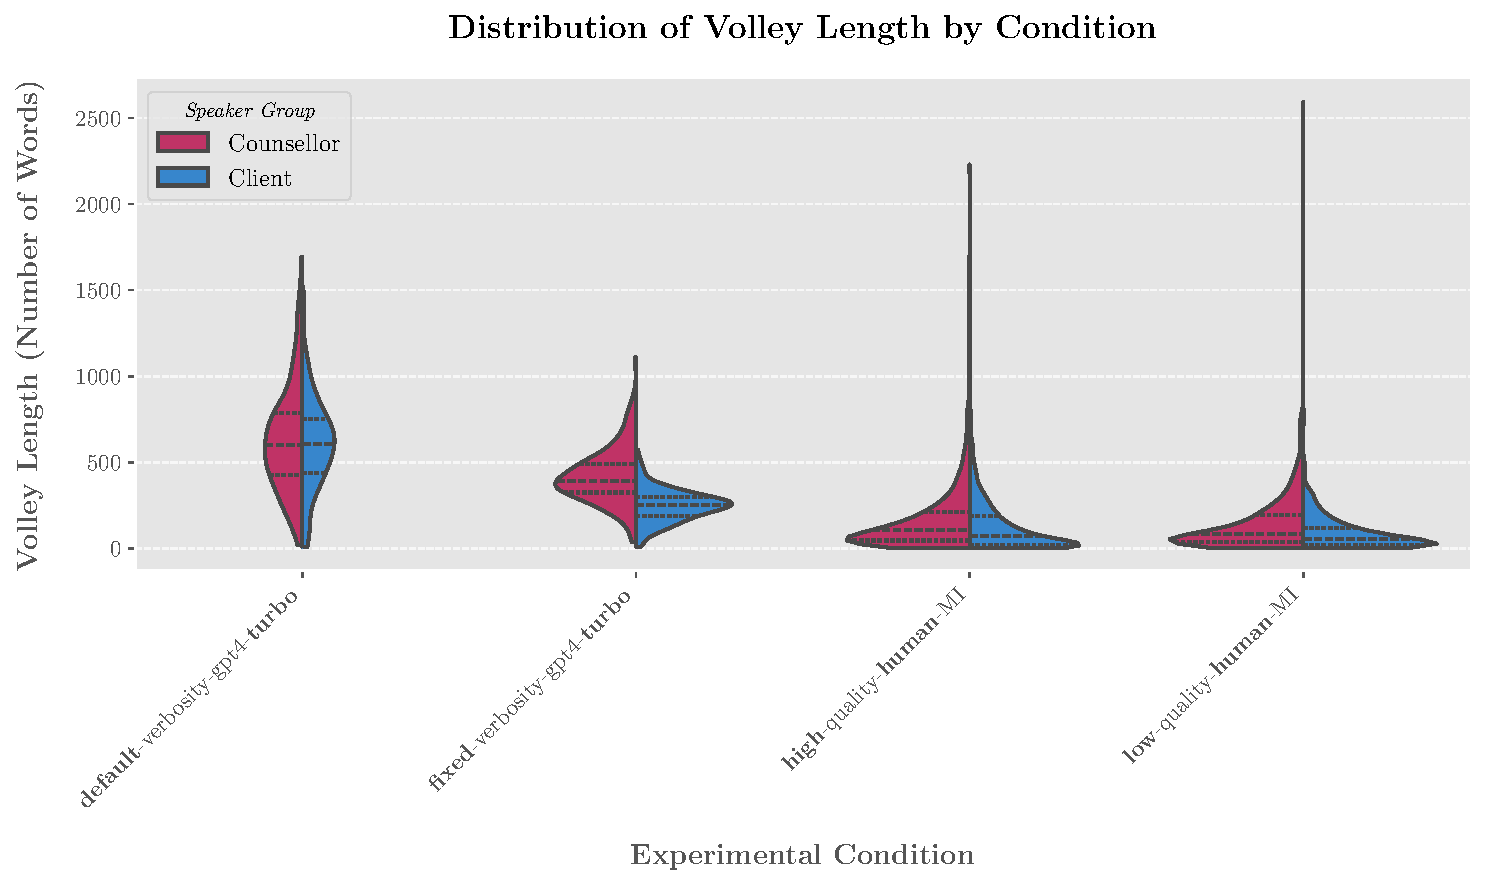
\includegraphics[width=0.9\textwidth]{fig/utterance_length_violin_plot.pdf}
    \caption[Distribution of volley length for default and fixed-verbosity synthetic smokers]{Comparison of utterance length distributions for default and fixed-verbosity synthetic smokers. The fixed-verbosity prompt successfully reduced the synthetic smoker's utterance length to better align with humans (\texttt{high-quality-human-MI})}
    \label{fig:verbosity-comparison}
\end{figure}

\begin{table}[ht]
\centering

\begin{tabular}{lrr}
\toprule
{} &  \textbf{Mean} &  \textbf{Standard Deviation} \\
\textbf{Category}                   &                        &           {}          \\
\midrule
Default Verbosity (GPT-4 Turbo) &                  618.9 &               296.3 \\
Fixed Verbosity (GPT-4 Turbo)   &                  337.8 &               157.9 \\
High-Quality Human Counselling             &                  147.0 &               172.9 \\
Low-Quality Human Counselling            &                  118.2 &               158.0 \\
\bottomrule
\end{tabular}
\caption{Statistics on Volley Length for Low- and High-Verbosity Synthetic Smokers.}
\label{tab:utterance_stats}
\end{table}

The default verbosity condition showed a wide distribution with a high median utterance length. The fixed-verbosity synthetic smokers successfully matched the utterance length distribution of humans from the HLQC dataset. \Cref{tab:utterance_stats} provides detailed statistics on the volley lengths.

Interestingly, we observed that the counsellor bot reciprocated the client's verbosity. When the synthetic smoker spoke less, the counsellor bot also reduced its utterance length. We also verified that these prompt modifications were robust and transferable across different LLMs (GPT-4 Turbo and GPT-4 Omni).

\subsection{Installing Resistance}
\label{sec:synthetic-smoker-resistance}

Addressing the baseline smoker's high agreeableness was crucial, as addressing resistance to change is a crucial MI skill.

\subsubsection{Methodology}
We hypothesized that resistance could be installed by providing the LLM with detailed backstories emphasizing different motivations and experiences. We created two distinct personas:

\begin{itemize}
    \item High Resistance Persona: The backstory emphasized severe life stressors, repeated failed quit attempts, skepticism towards therapy, and a strong belief that it was not the right time to quit.
    \item Low Resistance Persona: The backstory described recent health concerns prompting contemplation, and an open, albeit skeptical, attitude towards change.
\end{itemize}

Using modified prompts and GPT-4 Turbo (temperature=1.0), we generated conversations (N=10 per persona) between synthetic smokers and MIBot. We employed two distinct methods to validate the installation. We also prompted these synthetic smokers to fill out the readiness rulers before, after, and a week after the conversation. We did so by prompting the synthetic smoker with the exact questions from the readiness rulers survey. Before reporting the numbers, we asked them to think and provide reasons for the numerical rating they chose before outputting the rating---a technique known as chain-of-thought prompting.

\subsubsection{Validation}

\begin{enumerate}
    \item Linguistic Evidence (Change vs. Sustain Talk): We analysed the transcripts to measure the proportion of Change Talk (CT) and Sustain Talk (ST).


    \item Behavioural Evidence (Self-Reported Readiness): We further validated the installation by asking the synthetic smokers to complete the Readiness Ruler survey (Importance, Confidence, and Readiness; 0--10 scale) before, immediately after, and \emph{simulated} one week after the conversation.

\end{enumerate}






\subsubsection{Results} 



\begin{table}[ht!]
\centering
\begin{tabular}{@{}llll@{}}
\toprule
\textbf{Persona} & \textbf{Change Talk (\%)} & \textbf{Sustain Talk (\%)} & \textbf{Neutral (\%)} \\ \midrule
High Resistance & 31 & 44 & 25 \\
Low Resistance & 61 & 9 & 30 \\ \bottomrule
\end{tabular}
\caption{\% Change, sustain, and neutral talk for high- and low-resistance synthetic smokers.}
\label{tab:resistance-ct-st}
\end{table}

\begin{table}[ht!]
  \centering
  \small
  \renewcommand{\arraystretch}{1.2} % Increased spacing slightly for readability
  \resizebox{\linewidth}{!}{\begin{tabular*}{\linewidth}{@{\extracolsep{\fill}}llcccc@{}}
    \toprule
    \textbf{} & \textbf{} & \textbf{Pre-} & \textbf{Post-} & \textbf{1-week} & \textbf{} \\
       
        \textbf{Client} & & \textbf{conversation} & \textbf{conversation} & \textbf{Follow-up} & \textbf{Change from} \\
        
    \textbf{Resistance}  &  \textbf{Variable} & \textbf{mean (SD)} & \textbf{mean (SD)} & \textbf{mean (SD)} & \textbf{Baseline} \\
    \midrule
    \multirow{3}{*}{Low} & Importance & 4.6 (0.5) & 5.4 (0.9) & 6.6 (0.5) & 2.0 (0.7) \\
    & Confidence & 2.6 (0.5) & 4.2 (1.1) & 4.8 (0.4) & 2.2 (0.4) \\
    & Readiness  & 3.2 (1.1) & 5.2 (1.1) & 5.4 (0.9) & 2.2 (1.9) \\
    \midrule
    \multirow{3}{*}{High} & Importance & 2.0 (0.0) & 4.0 (0.7) & 4.6 (1.1) & 2.6 (1.1) \\
    & Confidence & 1.0 (0.0) & 2.0 (0.0) & 2.6 (0.9) & 1.6 (0.9) \\
    & Readiness  & 0.6 (0.5) & 2.6 (0.5) & 3.4 (1.1) & 2.8 (1.1) \\
    \bottomrule
  \end{tabular*}}
  \caption[Readiness rulers reported by high- and low-resistance synthetic smokers]{Longitudinal changes in self-reported scores (0--10 scale) for importance, confidence, and readiness, stratified by client (synthetic smoker) resistance level. Values were assessed at baseline (pre-conversation), immediately post-conversation, and at 1-week follow-up. Change scores represent the difference between baseline and 1-week follow-up. SD = standard deviation}
  \label{tab:resistance-readiness-rulers}
\end{table}


The analysis confirmed a clear distinction between the two personas (\Cref{tab:resistance-ct-st}). The High Resistance smoker used significantly more Sustain Talk (44\% vs. 9\%) and less Change Talk (31\% vs. 61\%) than the Low Resistance smoker.


The readiness ruler scores demonstrated that the synthetic smokers provided responses consistent with their installed resistance levels (\Cref{tab:resistance-readiness-rulers}). The ``high-resistance'' synthetic smokers reported lower mean scores on all three dimensions of the readiness rulers. Interestingly, their week-later change in confidence was lower than ``low-resistance'' smokers by 0.8 points, while the change in importance and readiness was slightly higher.




This experiment also provided us with our first evidence that LLM-based synthetic smokers could self-report their smoking behaviours numerically and that the numbers were consistent with the installed attributes. We did notice, however, that the variability of scores was much lower---especially for pre-conversation readiness numbers---as the only source of stochasticity among these agents was the decoding temperature of the underlying LLM.



\section{Conclusion}
\label{sec:prelim-conclusion}

The preliminary experiments detailed in this chapter successfully established a foundation for creating synthetic smokers. We demonstrated that through prompt engineering, it is possible to control basic conversational attributes such as \textbf{verbosity} and install psychological constructs like \textbf{resistance}. Through our validation methods, which included linguistic analysis (\%CT) and behavioural self-reports (readiness rulers), we confirmed that these installed attributes were reflected in the agents' outputs.

These initial studies, however, also revealed significant limitations. The personas were created with arbitrary backstories, which made it difficult to assess the \textbf{representativeness} of our synthetic population against a real-world target demographic. Validating the \textbf{fidelity} of these agents remained a challenge without a direct human counterpart for comparison. To address these issues and move towards a more rigorous validation framework, we needed a data-driven approach. The next chapter introduces the ``doppelgänger'' methodology, a technique designed to create synthetic twins of actual human participants, allowing for a direct and robust assessment of our system's fidelity and representativeness.
\chapter{Advanced Methods for Attribute Installation in Synthetic Smokers}
\label{ch:synthetic-doppelgänger}

As established in the previous chapter, creating personas with arbitrary backstories made it difficult to rigorously assess the \textbf{representativeness} and \textbf{fidelity} of our synthetic agents. To overcome these limitations, we developed the ``doppelgänger'' methodology—a data-driven approach designed to create synthetic twins of actual human participants, enabling a more direct and robust validation framework.

This method leverages a rich dataset from a previous feasibility study on human smokers using MIBot v6.3A (see \Cref{ch:feasibility}), which we refer to by the shorthand \textbf{MIV6.3A}. The dataset contains 106 complete MIBot--human interactions, including demographic data, smoking history (e.g., Heaviness of Smoking Index---HSI), pre- and post-conversation readiness rulers (\emph{importance}, \emph{confidence}, \emph{readiness}), and full conversation transcripts. By extracting and installing attributes directly from this human data, we can create doppelgängers that mirror a real-world distribution. This chapter details the specific methods for creating and evaluating these synthetic doppelgängers.

\section{The Doppelgänger Methodology: A Data-Driven Approach}
\label{sec:synthetic-smoker-doppelgänger}


Without installing a diverse set of attributes from a target population, it became challenging to validate our development of synthetic smokers in terms of distributional representativeness and uniform fidelity. 
Therefore, we utilized the data from the feasibility study on human smokers using MIBot v6.3A (\Cref{ch:feasibility}) to extract installable attributes. This study provided a rich dataset of 106 MIBot--human interactions, including pre- and post-conversation readiness rulers (\emph{importance}, \emph{confidence}, \emph{readiness}), demographic data, smoking history (e.g., Heaviness of Smoking Index---HSI), and complete conversation transcripts. Throughout the rest of this chapter, we refer to this dataset by the shorthand \textbf{MIV6.3A}.

The dataset enabled a shift from creating synthetic smokers with an arbitrary attribute distribution to one drawn from MIV6.3A. We explicitly controlled for certain attributes, such as ensuring an equal number of male and female participants before applying confidence screening. Thus, the creation of doppelgängers allowed us to validate our methodology more rigorously.

For the rest of our discussion, we define a doppelgänger as a synthetic smoker designed to be a ``behavioural twin'' of a specific human participant from the feasibility study, although this definition can be extended to other types of participants and studies. The goal is to create an agent that, when exposed to MI counselling, behaves similarly to its human counterpart in terms of language use, psychological profile, and changes in readiness to quit.

Using the doppelgänger methodology provides a straightforward approach to validating the fidelity of synthetic smokers. Rather than using a method $M$ to approximate installed attributes $\hat{\textbf{A}}_S$ from an observation $\gamma_S$, we can devise a robust and clinically grounded classifier ($\textbf{C}$) that operates on $\gamma$. For example, we can calculate the fraction of change talk (\%CT) from the transcripts.

Further, we can use this classifier to find the distance $d(\textbf{C}(\gamma_H), \textbf{C}(\gamma_S))$. Since, in the case of doppelgängers, $\textbf{A}_S = \textbf{A}_H$, we can approximate the fidelity as:

$$\hat{\mathcal{F}}(\textbf{A}^\textbf{C}) = \mathbb{E}_{\gamma_H \sim P_H (\gamma | \textbf{A}_H),  \:  \gamma_S \sim P_S(\gamma | \textbf{A}_H)}[d(
\textbf{C}(\gamma_H),\textbf{C}(\gamma_S)
)]$$


where $\textbf{A}^\textbf{C} = \{a \in \textbf{A} \mid a \sim \textbf{C}(\gamma)\}$. For example, if the correlation between the \%CT of human and synthetic smokers is high, this can approximate the fidelity, $\hat{\mathcal{F}}$. One drawback is that this kind of validation can only measure whether certain attributes are installed and evidenced in the language. It cannot provide a complete picture of fidelity across all attributes. Hence, it approximates the fidelity over a small subset of attributes, $\textbf{A}^\textbf{C}$, i.e., those attributes that are discernible by the classifier $\textbf{C}(\gamma)$.



\section{The Conversational Impact Modelling Experiment}
\label{sec:transcript-autoplay}

Before attempting to install attributes in doppelgängers and have them engage in novel conversations with MIBot, we needed to establish a baseline understanding of the LLM's ability to model the psychological impact of a conversation and contextualize numerical readiness rulers with other installed attributes. For this purpose, we designed the ``Conversational Impact Modelling'' experiment.

If an LLM-based synthetic smoker (a doppelgänger) is given the pre-conversation attributes of a human participant and the exact transcript of the MIBot--human conversation (acting as if the doppelgänger itself is speaking the human's lines), can it accurately report the same post-conversation readiness rulers as the human?

\subsubsection{Methodology}
\begin{enumerate}
    \item Install the pre-conversation attributes of a specific human participant in the doppelgänger.
    \item Feed the transcript of the actual conversation sequentially to the doppelgänger, framing it as a dialogue in which the doppelgänger is participating.
    \item After the conversation concludes, ask the doppelgänger to complete the post-conversation readiness rulers.
\end{enumerate}

In other words, the doppelgänger was provided with the participant's actual pre-conversation readiness rulers (importance, confidence, and readiness) and the full transcript of their conversation with MIBot. After processing this information, the doppelgänger was asked to report its post-conversation readiness rulers.

The doppelgänger was given the system prompt detailed in Appendix~\ref{app:doppelganger-prompts}. An excerpt is shown below:

\includesystemprompt{Conversational Impact Modelling Prompt}{
You are a participant in a study who is trying to quit smoking.\\
Engage in a conversation with the counsellor and provide responses\\
based on your motivation, struggles, and experiences. Your assistant\\
role is the client, and the user's role is the counsellor or\\
the researcher.\\\\
Before you talk to the counsellor, please answer the following
questions. \\\\
\quad On a scale from 0 to 10, how important is it to you right\\
now to stop smoking? Respond with a single integer between 0 (very\\
low importance) and 10 (very high importance).\\\\
...
}

To investigate the doppelgänger's reasoning process and potentially improve its accuracy, we utilized several prompting techniques:

\begin{enumerate}
    \item \textbf{Baseline:} A standard prompt asking the doppelgänger for the post-conversation score.
    \item \textbf{Chain-of-Thought (CoT):} An enhanced prompt that required the doppelgänger to articulate its reasoning by reflecting on the conversation's key insights, its own motivations, and any expressed shifts in perspective before providing the final numerical score.
\end{enumerate}

We tested this methodology with multiple underlying models, including GPT-4o and Claude 3.7 Sonnet. For the Claude model, we also leveraged its native ``thinking'' feature, which allows the doppelgänger to perform an internal monologue and reflection before generating a final answer, serving as a functional alternative to an explicit CoT prompt.

\subsubsection{Evaluation}
The primary evaluation metrics were the Mean Absolute Error (MAE), Mean Squared Error (MSE), and Spearman's correlation ($r$) between the human-reported and doppelgänger-reported outcomes.

\subsubsection{Results}
First, to establish a performance benchmark, a simple linear regression model was created to predict post-conversation confidence using only pre-conversation confidence from the human data. This yielded an \textbf{MSE of 3.2}, representing the baseline accuracy achievable without considering the conversational content.

The Conversational Impact Modelling experiments consistently outperformed this simple baseline, demonstrating the doppelgänger's ability to extract meaningful signals from the conversation transcripts. An initial ablation study, summarized in \Cref{tab:ablation_results}, reveals the importance of providing the doppelgänger with both the pre-conversation context and the transcript.



\begin{table}[ht!]
\centering
\begin{tabular}{@{}lrr@{}}
\cmidrule(r){1-2}
\textbf{Input Provided to GPT-4o} & \textbf{Mean Squared Error (MSE)} & \\
\cmidrule(r){1-2}
Transcript ONLY & 5.5 & \\
Pre-Conversation Confidence ONLY & 3.7 & \\
\textcolor{gray}{Linear Regression (Pre-Conf. $\rightarrow$ Post-Conf.)} & \textcolor{gray}{3.2} & \textcolor{red}{\small $\leftarrow$ Baseline} \\
Pre-Conversation Confidence + Transcript & 3.1 & \\
\textbf{Full Pre-Conversation Rulers + Transcript} & \textbf{2.9} & \\
\cmidrule(r){1-2}
\end{tabular}
\caption[Ablation study on doppelgängers' self-reported post-conversation confidence]{Impact of different attributes on GPT-4o-based doppelgängers' self-reported post-conversation confidence. Both the pre-conversation readiness rulers and the conversation transcript are necessary for the doppelgängers to accurately report post-conversation confidence.}
\label{tab:ablation_results}
\end{table}



While metrics like MAE provide a quantitative summary, a visual comparison of the distributions reveals some discrepancies. \Cref{fig:post_conf_distributions} plots the distribution of human-reported confidence scores alongside the distribution of GPT-4o-based doppelgänger. Both distributions are similarly left-skewed, indicating that the model correctly identifies that most participants land in the higher-confidence range (6--10). However, the doppelgänger predictions were less varied than the human responses. The human data shows a broader plateau of high confidence across scores of 6, 7, and 8, whereas the doppelgängers exhibit a pronounced peak at a score of 7. This suggests that while the model is effective at capturing the overall positive trend, it may be less sensitive to the subtle individual differences in participants' final confidence levels, tending to revert to a more common or ``average'' high-confidence outcome.



\begin{figure}[ht!]
    \centering
    \begin{minipage}{0.48\textwidth}
        \centering
        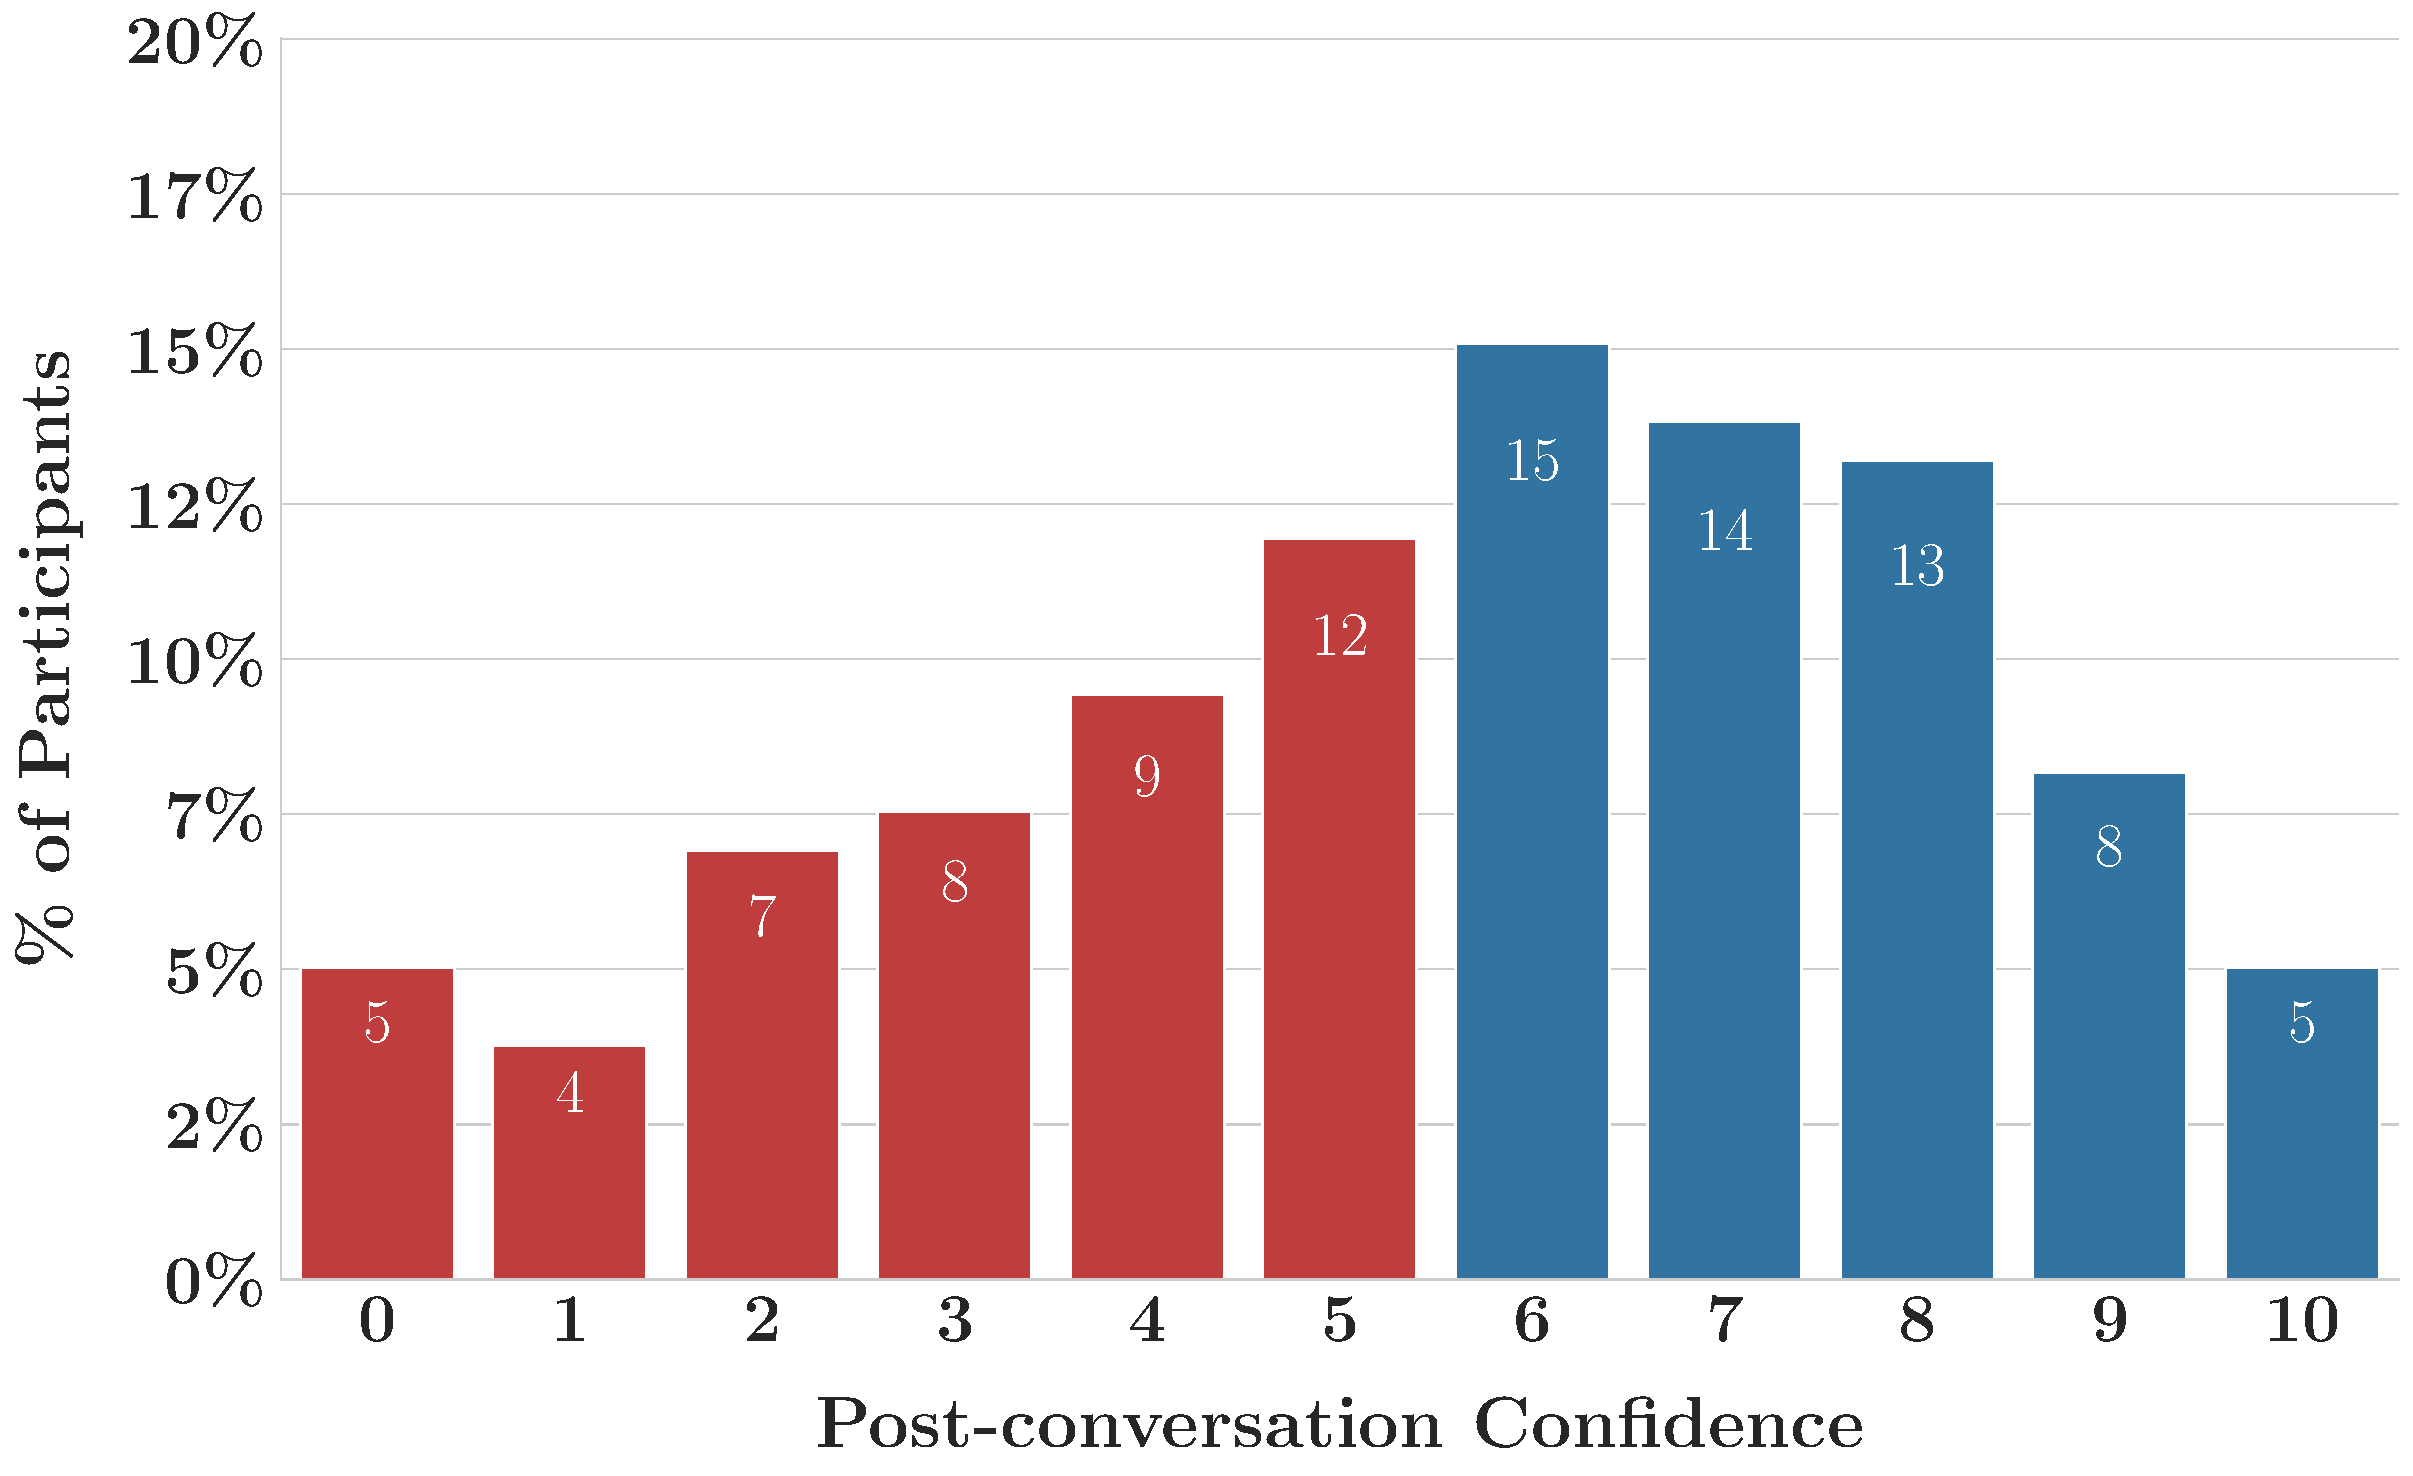
\includegraphics[width=\linewidth]{fig/post-conf-human.pdf}
        \subcaption{Human-reported post-conversation confidence scores}
        % No sub-caption needed as the main caption explains it
    \end{minipage}\hfill
    \begin{minipage}{0.49\textwidth}
        \centering
        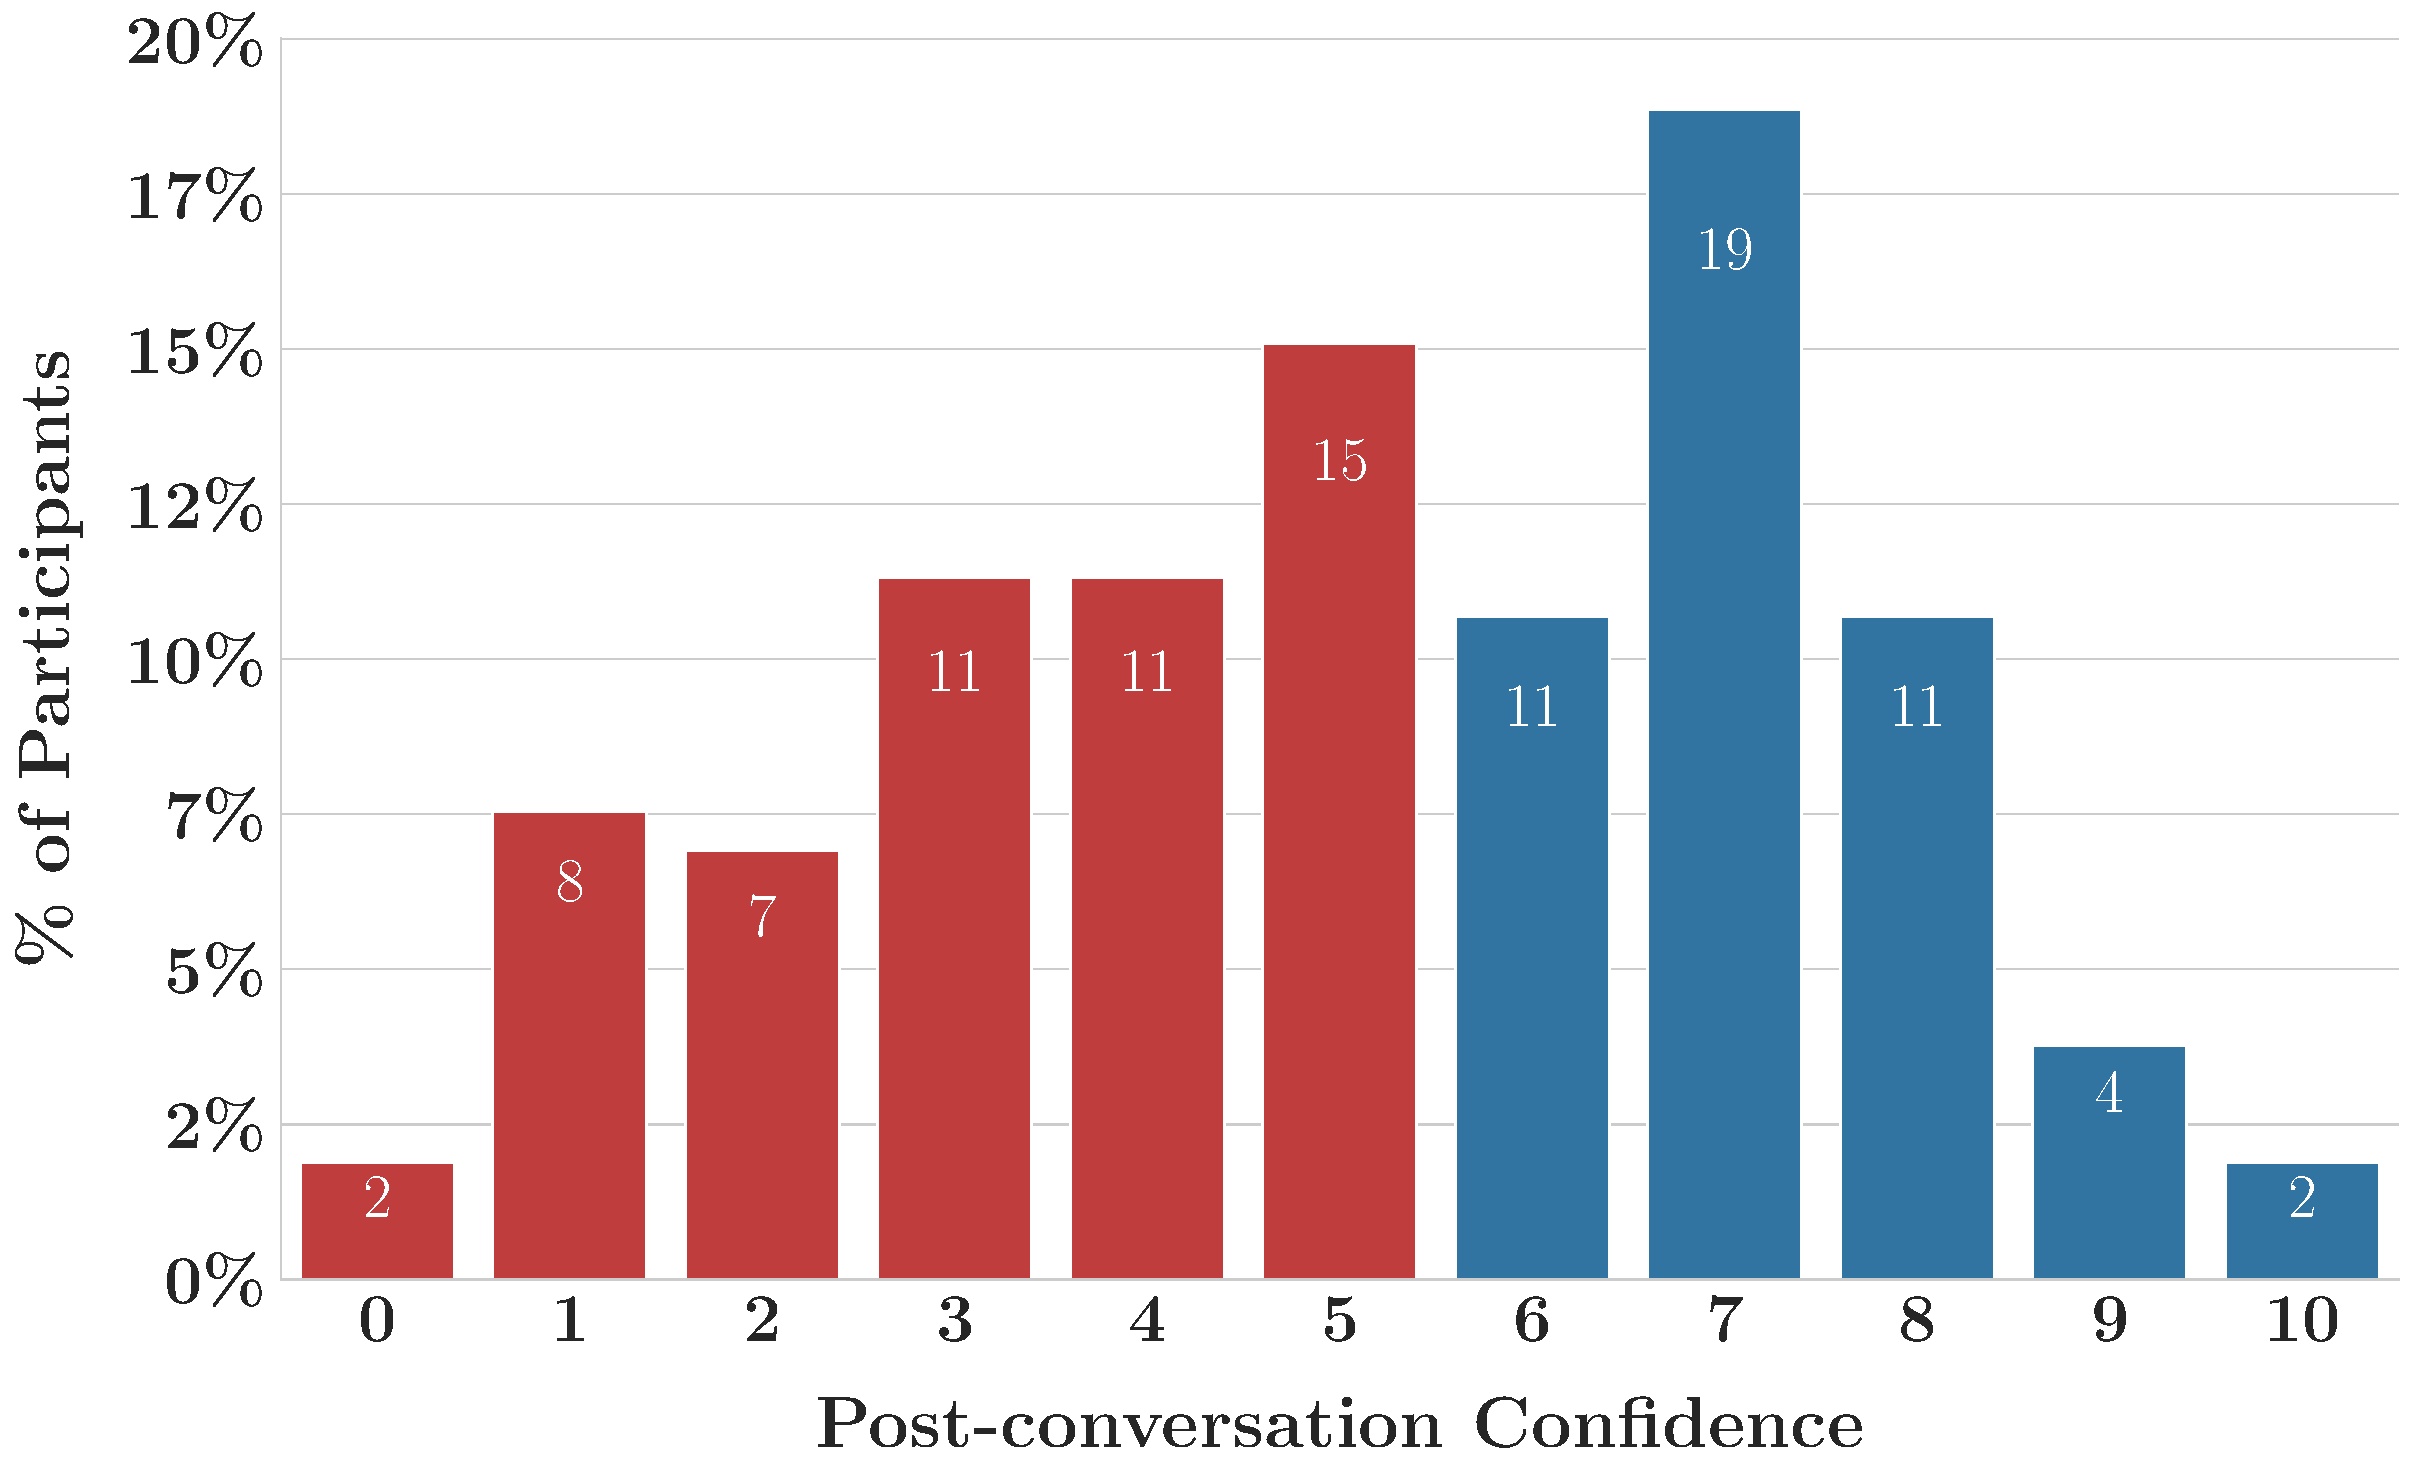
\includegraphics[width=\linewidth]{fig/post-conf-gpt4-o.pdf}
        \subcaption{Doppelgänger-reported post-conversation confidence scores}
    \end{minipage}
    \caption{Distribution of post-conversation confidence scores. While the overall shapes are similar, the doppelgänger's scores are more concentrated around a single peak (score of 7), whereas human responses are more distributed across several high-confidence values.}
    \label{fig:post_conf_distributions}
\end{figure}


Next, we compared the performance of different underlying models and prompting techniques used by the doppelgängers to report post-conversation confidence. The results, detailed in \Cref{tab:model_comparison}, show that reflective prompting methods consistently improved accuracy.


\begin{table}[!ht]
\centering
\begin{tabular}{l|cccc}
\toprule
\textbf{Model} & \textbf{MAE} & \textbf{MSE} & \textbf{Correlation ($r$)} & \textbf{Exact Matches (\%)} \\
\midrule
GPT-4o (Baseline) & 1.2 & 3.0 & 0.7 & 31
\\
GPT-4o (CoT) & 1.2 & 2.9 & 0.7 & 30 \\
Claude 3.7 Sonnet (CoT) & 1.2 & 2.7 & 0.7 & 31 \\
\textbf{Claude 3.7 Sonnet (Thinking)} & \textbf{1.1} & \textbf{2.6} & \textbf{0.8} & \textbf{32} \\ 
\bottomrule
\end{tabular}
\caption[Effect of LLM type and reasoning on synthetic smokers' self-reported confidence.]{Comparison of different models and prompting techniques and their impact on the self-reporting of post-conversation confidence (N=159). Reflective techniques, especially Claude 3.7 Sonnet's ``thinking'' feature, yielded the best results across all metrics.}
\label{tab:model_comparison}
\end{table}

The baseline GPT-4o doppelgänger achieved a strong correlation of \textbf{$r=0.7$} with the human-reported scores. However, the \textbf{Claude 3.7 Sonnet doppelgänger using its ``thinking'' feature achieved the lowest error (MAE=1.1, MSE=2.6) and the highest correlation ($r=0.8$)}.


\begin{figure}[htpb]
    \centering
    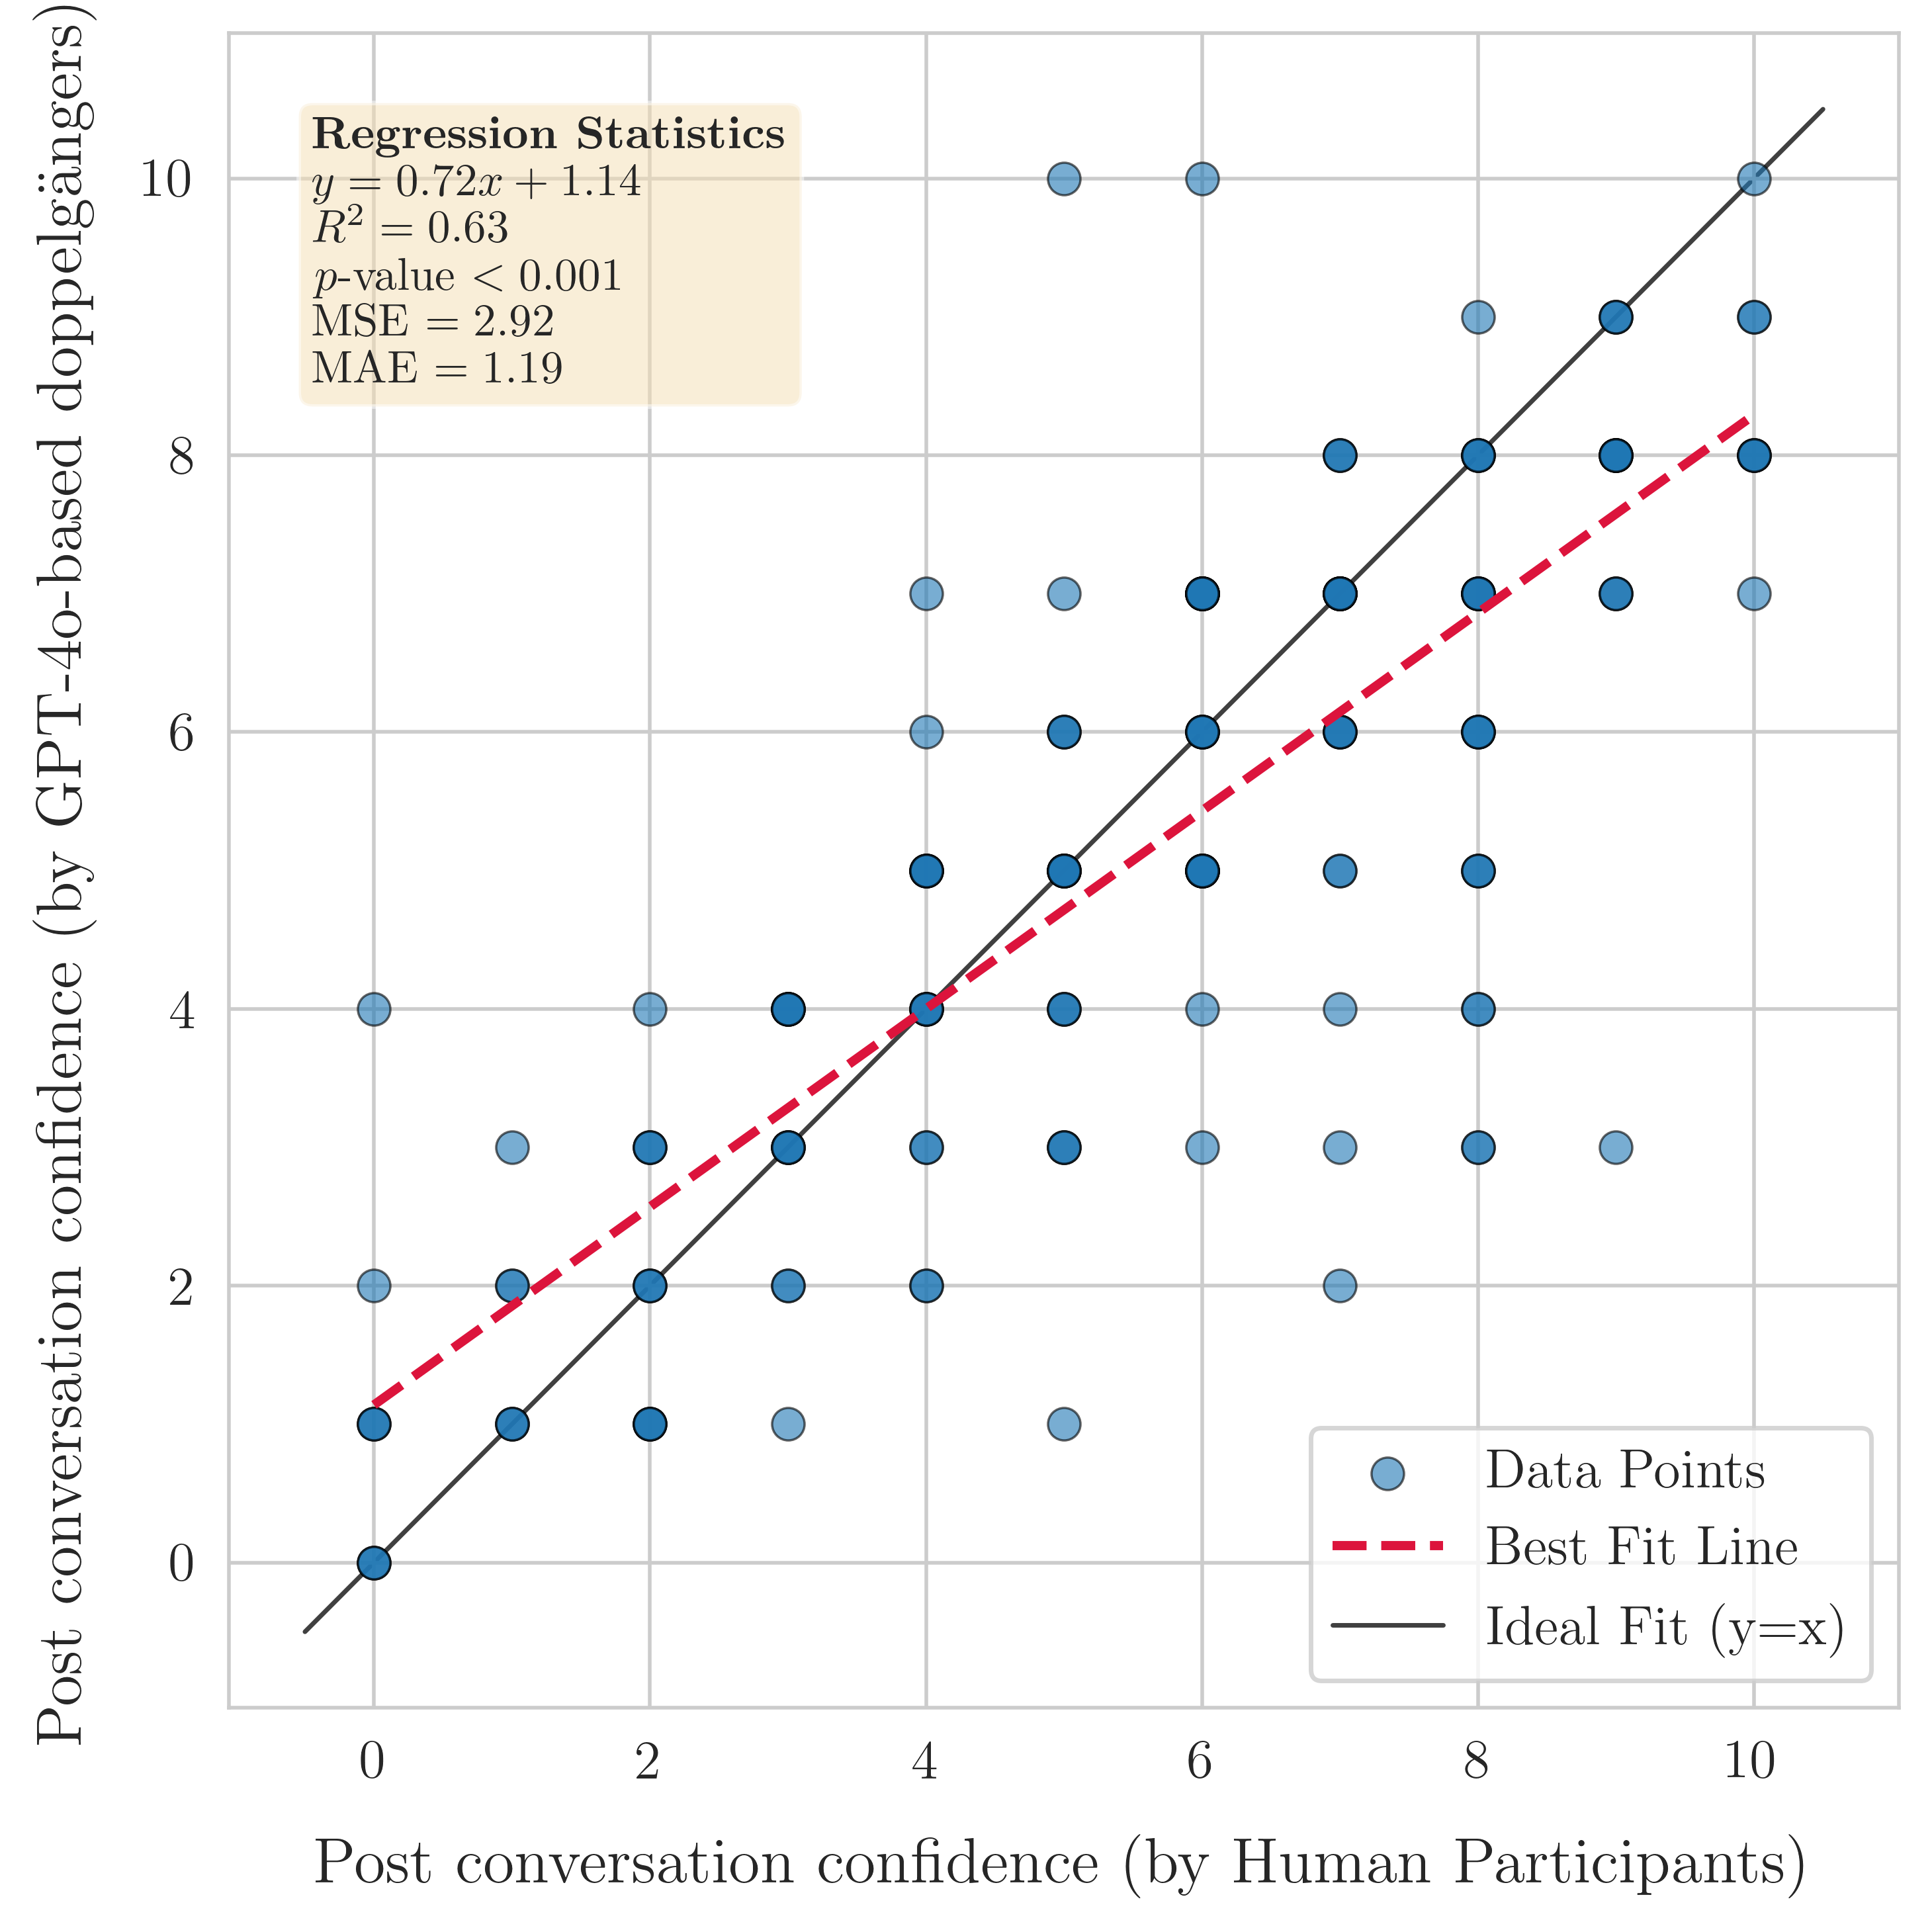
\includegraphics[width=0.5\textwidth]{fig/post_conf_gpt4o_vs_human.png}
    \caption{Scatter plot of human-reported vs. doppelgänger-reported post-conversation confidence for the baseline GPT-4o model, showing a Spearman's correlation of r=0.70. The diagonal line represents perfect agreement.}
    \label{fig:post-conf-gpt4o-vs-human}
\end{figure}


\Cref{fig:post-conf-gpt4o-vs-human} visualizes the relationship between the post-conversation confidence reported by human participants and that reported by their corresponding GPT-4o-based doppelgängers. The analysis reveals a strong, statistically significant positive correlation (Spearman's $r=0.70, p < 0.001$), indicating that the doppelgängers are generally successful in mirroring the human outcomes after processing the conversation transcript. The Mean Absolute Error (MAE) was 1.19, suggesting the doppelgänger's reported score was typically within about 1.2 points of the human's score on the 0--10 scale.

However, the plot also reveals a notable trend when comparing the best-fit line (dashed red) with the ideal fit (solid black). The regression equation ($y=0.72x+1.14$) shows a slope less than 1.0 and a positive intercept. This indicates a tendency towards ``regression to the mean'' in the doppelgänger reports. Specifically, when human participants reported very low confidence (e.g., 0--3), the doppelgängers tended to report slightly higher confidence (closer to the intercept of 1.14). Conversely, when humans reported very high confidence (e.g., 8--10), the doppelgängers tended to report slightly lower confidence. This suggests that while the directional impact of the conversation is captured well, the magnitude of the impact at the extremes might be slightly attenuated in the synthetic agents.

We further extended this analysis to include the other two readiness rulers: importance and readiness. The results are summarized in \Cref{tab:autoplay_results_full}.




\begin{table}[!ht]
\centering
\begin{tabular}{l|cc|cc|cc}
\toprule
& \multicolumn{2}{c|}{\textbf{Post-Confidence}} & \multicolumn{2}{c|}{\textbf{Post-Importance}} & \multicolumn{2}{c}{\textbf{Post-Readiness}} \\
\textbf{Model} & \textbf{MAE} & \textbf{Corr.} & \textbf{MAE} & \textbf{Corr.} & \textbf{MAE} & \textbf{Corr.} \\ 
\midrule
GPT-4o (CoT) & 1.2 & 0.7 & 0.8 & 0.9 & 0.7 & 0.9 \\
Claude 3.7 (Thinking) & 1.1 & 0.8 & 0.7 & 0.9 & 0.9 & 0.8 \\ \hline
\end{tabular}
\caption[Multi-ruler conversational impact modelling results]{Results of the conversational impact modelling experiment across all three readiness rulers, showing MAE and Pearson correlation. Performance was consistently strong, especially for importance and readiness.}
\label{tab:autoplay_results_full}
\end{table}

\Cref{tab:autoplay_results_full} summarizes the performance of the Conversational Impact Modelling experiment across all three readiness rulers. The results demonstrate high correlations (ranging from 0.7 to 0.9) across all rulers for both GPT-4o and Claude 3.7 models, affirming the robustness of the methodology.

It is interesting to note that the performance metrics for post-importance and post-readiness are generally stronger than for post-confidence. For example, the correlations for importance (0.9 for both models) are notably higher, and the MAEs are lower than for confidence. This suggests that the doppelgängers found it easier to accurately model the conversational impact on a participant's sense of importance and readiness to quit than on their self-efficacy (confidence) in their ability to do so. Overall, the Claude 3.7 model utilizing its ``thinking'' feature demonstrated slightly better performance in modelling confidence (correlation 0.8, MAE 1.1) compared to GPT-4o (correlation 0.7, MAE 1.2).



This experiment served as a check on the doppelgänger's ability to infer the psychological state resulting from the conversation. The underlying model possesses the necessary reasoning capabilities to allow the doppelgänger to understand how conversational dynamics influenced the participant's motivation and confidence. This serves as a baseline to confirm the doppelgänger's internal consistency before attempting to generate the conversation itself.



\section{Experiments with the Incremental Installation of Attributes}
Having gained insights into the LLM's ability to model conversations and its intuitive understanding of numerical attributes such as readiness rulers, we set out to systematically install attributes in LLM-based synthetic smokers and validate their installation. Recall from our discussion on the benefits of creating doppelgängers (\Cref{sec:synthetic-smoker-doppelgänger}). They provide a way to approximate the fidelity of an installation and make the validation of synthetic agents easier. We can approximate the fidelity of synthetic smokers with the correlation between some metric on the observable outer space (e.g., transcripts) of doppelgängers and their human twins. As an example, to validate whether the behavioural attribute of resistance to change has been successfully installed, we can analyze the transcripts from both humans and their doppelgängers and calculate the correlation between the percentage of Change Talk (\%CT) exhibited by both groups. A high correlation would then suggest a successful installation of this attribute.


\subsection*{Percentage Change Talk: A Key Metric for Validating Behavioural Fidelity}

To validate the synthetic smokers developed using the doppelgänger method, we needed an objective metric that could measure the smokers' level of motivation from their language.
We identified the percentage change talk metric (also referred to as change fraction or CF, calculated as CT / (CT + ST)) to fit our requirements, as it is grounded in the client's language and is strongly associated with behavioural change outcomes in MI \cite{Barnett2014,Houck2018,Moyers2009,Baer2008}.
Furthermore, we tested if \%CT is a valid proxy for a client's internal state, i.e., if it correlates with established metrics of readiness in human participants.

We analyzed the data from MIV6.3A ($N=106$ participants). The analysis confirmed strong, statistically significant correlations between \%CT and all readiness rulers (\Cref{tab:ct-correlation}). For example, the correlation with post-conversation confidence was 0.41 ($p < 0.0001$). These results motivated us to use \%CT as a primary metric for validating the installation of behavioural attributes in the synthetic smoker.


\begin{table}[!ht]
\centering
\begin{tabular}{@{}lr@{}}
\toprule
\textbf{Attribute} & \textbf{Correlation with \%CT} \\
\midrule
Pre-conversation importance & 0.47$^{****}$ \\
Pre-conversation confidence & 0.29$^{**}$ \\
Pre-conversation readiness & 0.46$^{****}$ \\
\midrule
Post-conversation importance & 0.49$^{****}$ \\
Post-conversation confidence & 0.41$^{****}$ \\
Post-conversation readiness & 0.48$^{****}$ \\
\midrule
Change in importance (Post--Pre) & 0.12 \\
Change in confidence (Post--Pre) & 0.24$^{**}$ \\
Change in readiness (Post--Pre) & 0.06 \\
\midrule
CARE (perceived empathy) & 0.15 \\
Previous number of quit attempts & 0.09 \\
Age & -0.11 \\
Number of cigarettes per day & -0.04 \\
HSI (Heaviness of Smoking Index) & -0.15 \\
\bottomrule
\multicolumn{2}{l}{\footnotesize{**** $p < 0.0001$, *** $p < 0.001$, ** $p < 0.01$, * $p < 0.05$}.}
\end{tabular}
\caption{Correlation between \%CT and human smoker attributes in the MIBot dataset.}
\label{tab:ct-correlation}
\end{table}



\subsection{Methodology}
The doppelgänger methodology uses a dataset of installable human attributes (e.g., MIV6.3A, containing attributes of human smokers) to build and validate synthetic smokers. The process involves:

\begin{enumerate}
    \item \textbf{Attribute Installation:} Instantiating a synthetic smoker, $S_i$, by installing the known attributes of a specific human participant, $H_i$, from the dataset. $A_S = A_H$. These attributes may include demographics, HSI, self-reported survey responses, etc.
    \item \textbf{Simulation:} The synthetic smoker, $S(A_H)$, interacts with the same counsellor (MIBot, in our case) that the original human interacted with.
    \item \textbf{Comparison:} The output of the synthetic smoker, $\gamma_S$, is compared with the actual output of the human, $\gamma_H$ (see \Cref{sec:synthetic-smoker-doppelgänger}).
\end{enumerate}



The overall workflow for creating and validating doppelgängers using this comparative method is illustrated in \Cref{fig:doppelgänger-creation-process}.



We created a set of doppelgängers (N=20) by sampling 20 human participants from MIV6.3A. Then, we conducted a series of experiments on these doppelgängers. In each experiment, we installed a subset of attributes in the doppelgängers via \emph{prompting} and did not add any backstories to their prompt.

\includesystemprompt{Example of attribute installation in doppelgänger prompts}{
You are a participant in a study who is trying to quit smoking. Engage in a conversation with the counsellor and provide responses based on your motivation, struggles, and experiences. Your assistant role is the client, and the user's role is the counsellor or the \\ researcher. Always try to respond in fewer than 200 characters. \\\\
About you: You are a 30-year-old female. You typically smoke 25 cigarettes per day. After you wake up, you smoke your first cigarette within 5 minutes. In the past week, you have not made any quit attempts.\\\\
Before speaking to the counsellor, you have rated your motivation to quit as follows (on a scale from 0 to 10): Importance: 2, Confidence: 0, Readiness: 4. \\\\
You talk about changing your smoking behaviour 46\% of the time.
...
}


Before starting our series of experiments, we sorted the set of all installable attributes based on their correlation with \%CT. We hypothesized that a high correlation between an attribute and \%CT would mean that the attribute has a bigger impact on the client's behavioural language. Let us call this sorted list of attributes $\mathbf{A'}$ (see Appendix~\ref{app:sorted-attributes-list} for the full list).

$$
\begin{aligned}
{\textbf{A}}^{'} = \{ & \text{pre-conversation importance,} \\
                     & \text{pre-conversation readiness,} \\
                     & \text{age,} \\
                     & \text{sex,} \\
                      & \text{pre-conversation confidence,} \\
                     \cdots \}
\end{aligned}
$$

The experiment then proceeds by incrementally adding attributes from this sorted list and, at each step, measuring the fidelity of the resulting doppelgängers. Fidelity is operationalized as the correlation between the percentage change talk (\%CT) of the human participants and their corresponding doppelgängers. The process is detailed in \Cref{alg:incremental_installation}.

{ 
\setstretch{1.25}
\begin{algorithm}[htpb]
    \caption{Incremental attribute installation and fidelity validation}
    \label{alg:incremental_installation}
    \begin{algorithmic}[1]
        \Require Human dataset $\mathcal{D} = \{ (H_i, \mathbf{A}_{H_i}, \gamma_{H_i}) \}_{i=1}^N$ containing human participants, their full attribute vectors, and conversation transcripts.
        \Require Sorted list of attributes $\mathbf{A'} = (a'_1, a'_2, \dots, a'_m)$ ordered by hypothesized relevance.\vspace{5pt}
        \State Initialize $\mathbf{A}_{\text{installed}} \leftarrow \emptyset$ \Comment{The set of attributes to install}
        \State Initialize $C \leftarrow ()$ \Comment{An empty list to store correlation results}

        \For{$k \leftarrow 1 \text{ to } m$} \Comment{Iterate through the sorted list of attributes}
            \State $\mathbf{A}_{\text{installed}} \leftarrow \mathbf{A}_{\text{installed}} \cup \{a'_k\}$ \Comment{Add the next attribute}
            
            \State Initialize $\mathbf{V}_{\text{human\_CT}} \leftarrow ()$ and $\mathbf{V}_{\text{synth\_CT}} \leftarrow ()$ \Comment{Vectors for \%CT scores}
            
            \For{$i \leftarrow 1 \text{ to } N$} \Comment{For each human participant in the dataset}
                \State $\mathbf{A}_{\text{subset}} \leftarrow \mathbf{A}_{H_i} |_{\mathbf{A}_{\text{installed}}}$ \Comment{Filter attributes for the current iteration}
                \State $S_i \leftarrow \mathcal{S}(\mathbf{A}_{\text{subset}})$ \Comment{Instantiate the synthetic smoker $S_i$ with the given parameters}
                \State Simulate a conversation between $S_i$ and MIBot to generate transcript $\gamma_{S_i}$.
                
                \State Calculate human \%CT: $c_{H_i} \leftarrow \text{\%CT}(\gamma_{H_i})$
                \State Calculate synthetic \%CT: $c_{S_i} \leftarrow \text{\%CT}(\gamma_{S_i})$
                
                \State Append $c_{H_i}$ to $\mathbf{V}_{\text{human\_CT}}$
                \State Append $c_{S_i}$ to $\mathbf{V}_{\text{synth\_CT}}$
            \EndFor
            
            \State Calculate the correlation for the current attribute set: $\rho_k \leftarrow \text{Correlation}(\mathbf{V}_{\text{human\_CT}}, \mathbf{V}_{\text{synth\_CT}})$
            \State Append $\rho_k$ to the results list $C$.
        \EndFor
        \vspace{5pt}
        \State \Return $C$ \Comment{A list of correlations, one for each incremental step of attribute installation}
    \end{algorithmic}
\end{algorithm}
}



\begin{figure}[htpb]
    \centering
    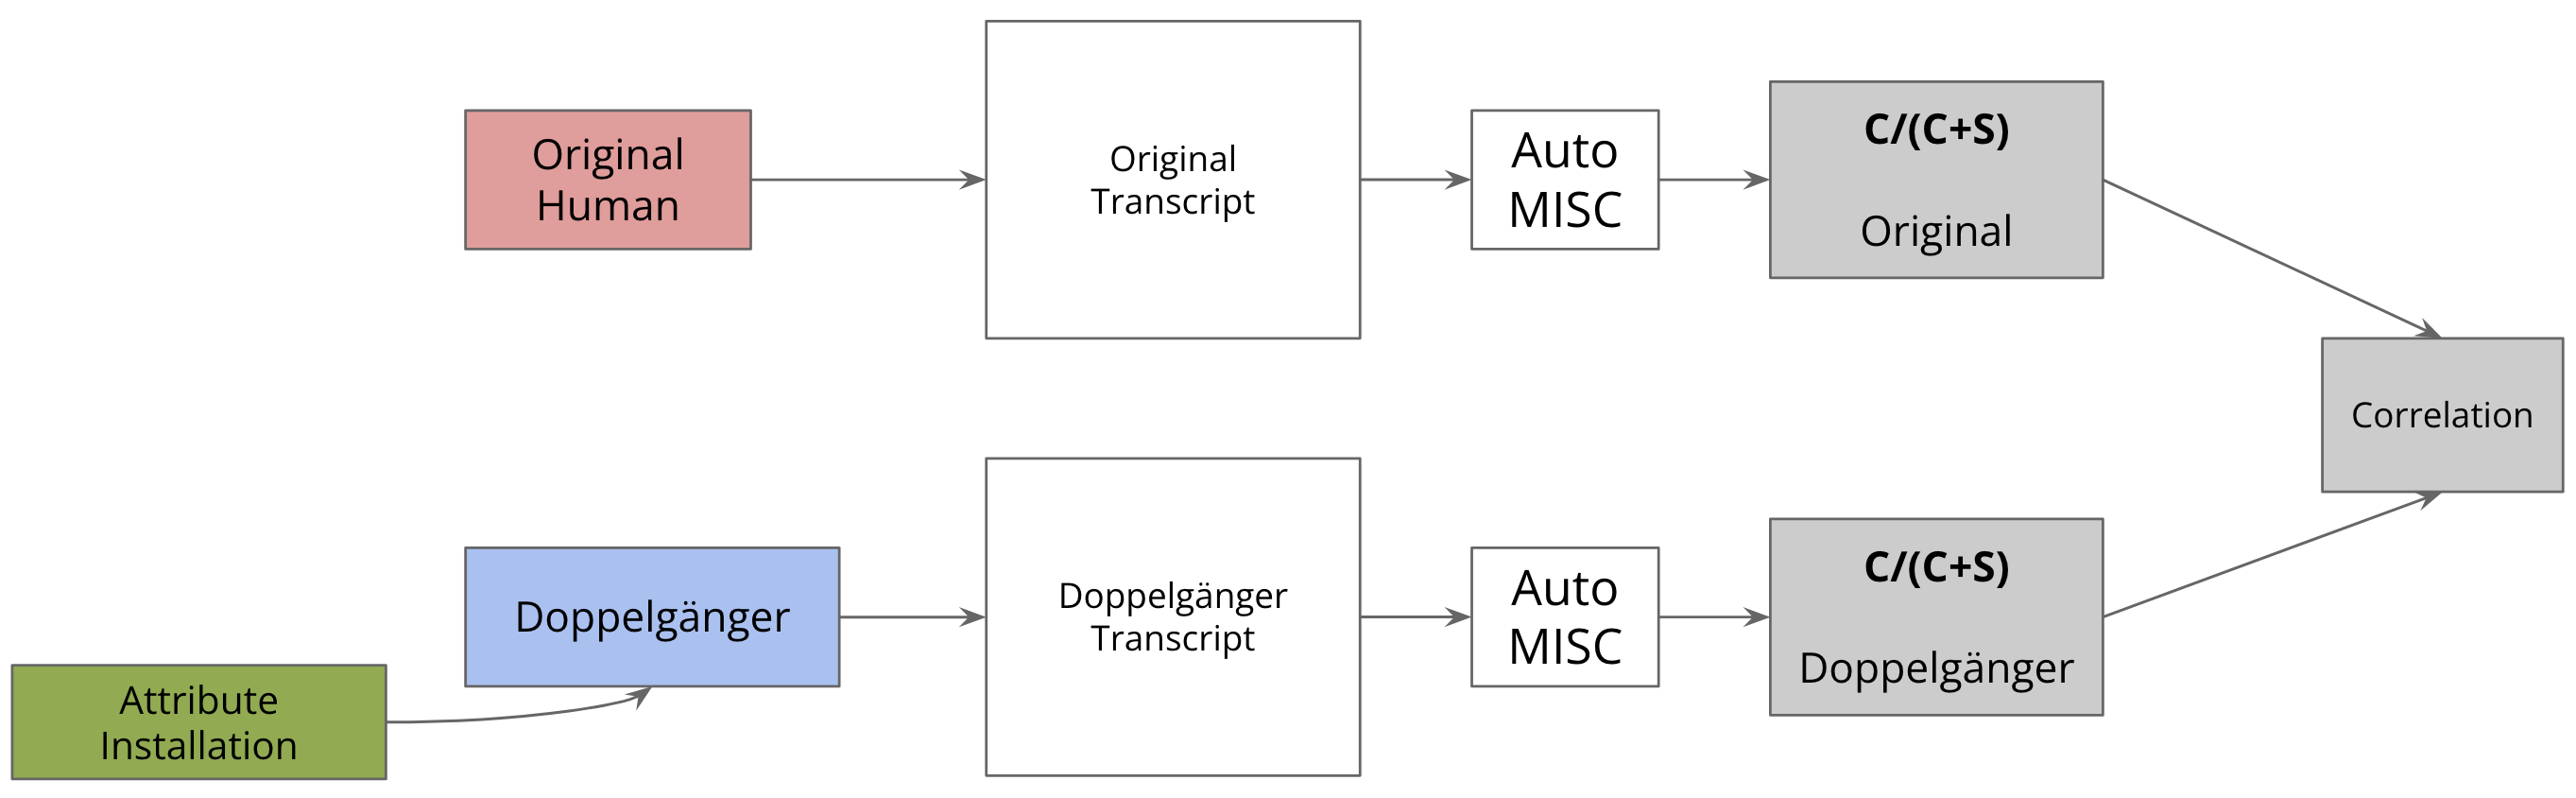
\includegraphics[width=0.98\textwidth]{fig/doppelganger_process.png}
    \caption{The doppelgänger creation and validation process. For each human participant ($H_i$), a synthetic twin ($S_i$) is created by installing their attributes ($A_{H_i}$). Both agents' conversations are analyzed to extract a behavioural metric (\%CT), and the correlation between the two sets of metrics is used to assess fidelity.}
    \label{fig:doppelgänger-creation-process}
\end{figure}


\subsection{Evaluation}
For each experiment with a set of attributes, we calculated the Spearman's correlation coefficient between the \%CT of human--MIBot and doppelgänger--MIBot conversations.



\subsection{Results}
The results of the incremental attribute installation are summarized in \Cref{tab:doppelgänger-correlations} (see Appendix~\ref{app:incremental-installation-data} for the full data). The fidelity, measured as the Spearman's rank correlation between the \%CT of humans and their doppelgängers, evolved as more attributes were added. Initially, adding attributes like pre-conversation importance and readiness led to a gradual increase in correlation. However, the process was not strictly monotonic; for instance, adding `pre-conversation confidence' in experiment 5 unexpectedly lowered the correlation from 0.40 to 0.22.

The most significant finding emerged in experiment 6, where explicitly installing the human's \%CT value as a numerical instruction resulted in a strong and statistically significant correlation of $r_s = 0.57$ ($p < 0.0001$). This suggests an LLM-based doppelgänger can directly operationalize a behavioural target when provided, modulating its language to match a specified proportion of change versus sustain talk.

However, despite achieving a strong rank correlation, a closer look at the population-level statistics reveals a systematic bias. As shown in the histograms in \Cref{fig:cf_comparison}, the distribution of \%CT for doppelgängers is shifted significantly higher than for humans (mean 0.76 vs. 0.59). The doppelgänger distribution is also more compressed and left-skewed, indicating a lower variance and a strong tendency to produce high levels of change talk, regardless of the human baseline.

This discrepancy is further visualized in the scatter plot in \Cref{fig:cf_human_vs_doppel}. While the points follow a positive trend that confirms the correlation, the majority lie above the identity line ($y=x$). This visually demonstrates that doppelgängers consistently overproduced change talk relative to their human counterparts. Even when a human participant had a low \%CT (e.g., below 0.4), their doppelgänger often produced a \%CT above 0.6 (see Appendix~\ref{app:doppelganger-transcript} for an example transcript).

Finally, we investigated the system's uniform fidelity by stratifying the results by sex, as detailed in \Cref{tab:doppelgänger-fidelity-sex}. While the mean \%CT for both human males and females was nearly identical ($\sim$59\%), the fidelity of their doppelgängers differed. The correlation for males ($r_s = 0.65$) was notably stronger than for females ($r_s = 0.52$), indicating a performance bias. This lack of uniform fidelity suggests the model may simulate one demographic group more accurately than another, an issue requiring further investigation to ensure representative synthetic populations. Other observations include:

\begin{enumerate}
    \item Once an attribute (e.g., pre-conversation importance) is installed in the doppelgängers, it is accurately recalled when prompted.
    \item Asking the doppelgängers to think before filling out the post-conversation readiness rulers reduced the gap (as measured by MAE) between their and human-reported scores.
\end{enumerate}



\begin{table}[ht!]
    \centering
    \begin{threeparttable}
    \sisetup{
        table-format=0.2,
        table-space-text-post = $^{****}$
    }
    \renewcommand{\arraystretch}{1.2}
    \begin{tabular}{c cccccc S}
        \toprule
        \textbf{Experiment} & \multicolumn{6}{c}{\textbf{Installed Attributes}} & {\textbf{\makecell{Spearman's rank \\ correlation}}} \\
        \cmidrule(r){2-7}
        & \makecell{Pre-conv. \\ importance} & \makecell{Pre-conv. \\ readiness} & Age & Sex & \makecell{Pre-conv. \\ confidence} & \%CT & {$r_s$} \\
        \midrule
        1 & \checkmark & & & & & & 0.19 \\
        2 & \checkmark & \checkmark & & & & & 0.24 \\
        3 & \checkmark & \checkmark & \checkmark & & & & 0.26 \\
        4 & \checkmark & \checkmark & \checkmark & \checkmark & & & 0.40 \\
        5 & \checkmark & \checkmark & \checkmark & \checkmark & \checkmark & & 0.22\tnote{*} \\
        6 & \checkmark & \checkmark & \checkmark & \checkmark & \checkmark & \checkmark & 0.57\tnote{****} \\
        \bottomrule
    \end{tabular}
    \begin{tablenotes}
        \footnotesize
        \item[*] $p < 0.05$
        \item[**] $p < 0.01$
        \item[***] $p < 0.001$
        \item[****] $p < 0.0001$
    \end{tablenotes}
    \end{threeparttable}
        \caption[Incremental attribute installation and its effect on the fidelity of doppelgängers.]{
        Incremental attribute installation and its effect on the fidelity of doppelgängers. Fidelity is measured by the Spearman correlation of percentage change talk (\%CT) between human participants and their doppelgängers (N=20). Each row represents a model where attributes were cumulatively added to the installation prompt.
    }
    \label{tab:doppelgänger-correlations}
\end{table}


\begin{figure}[ht!]
    \centering
    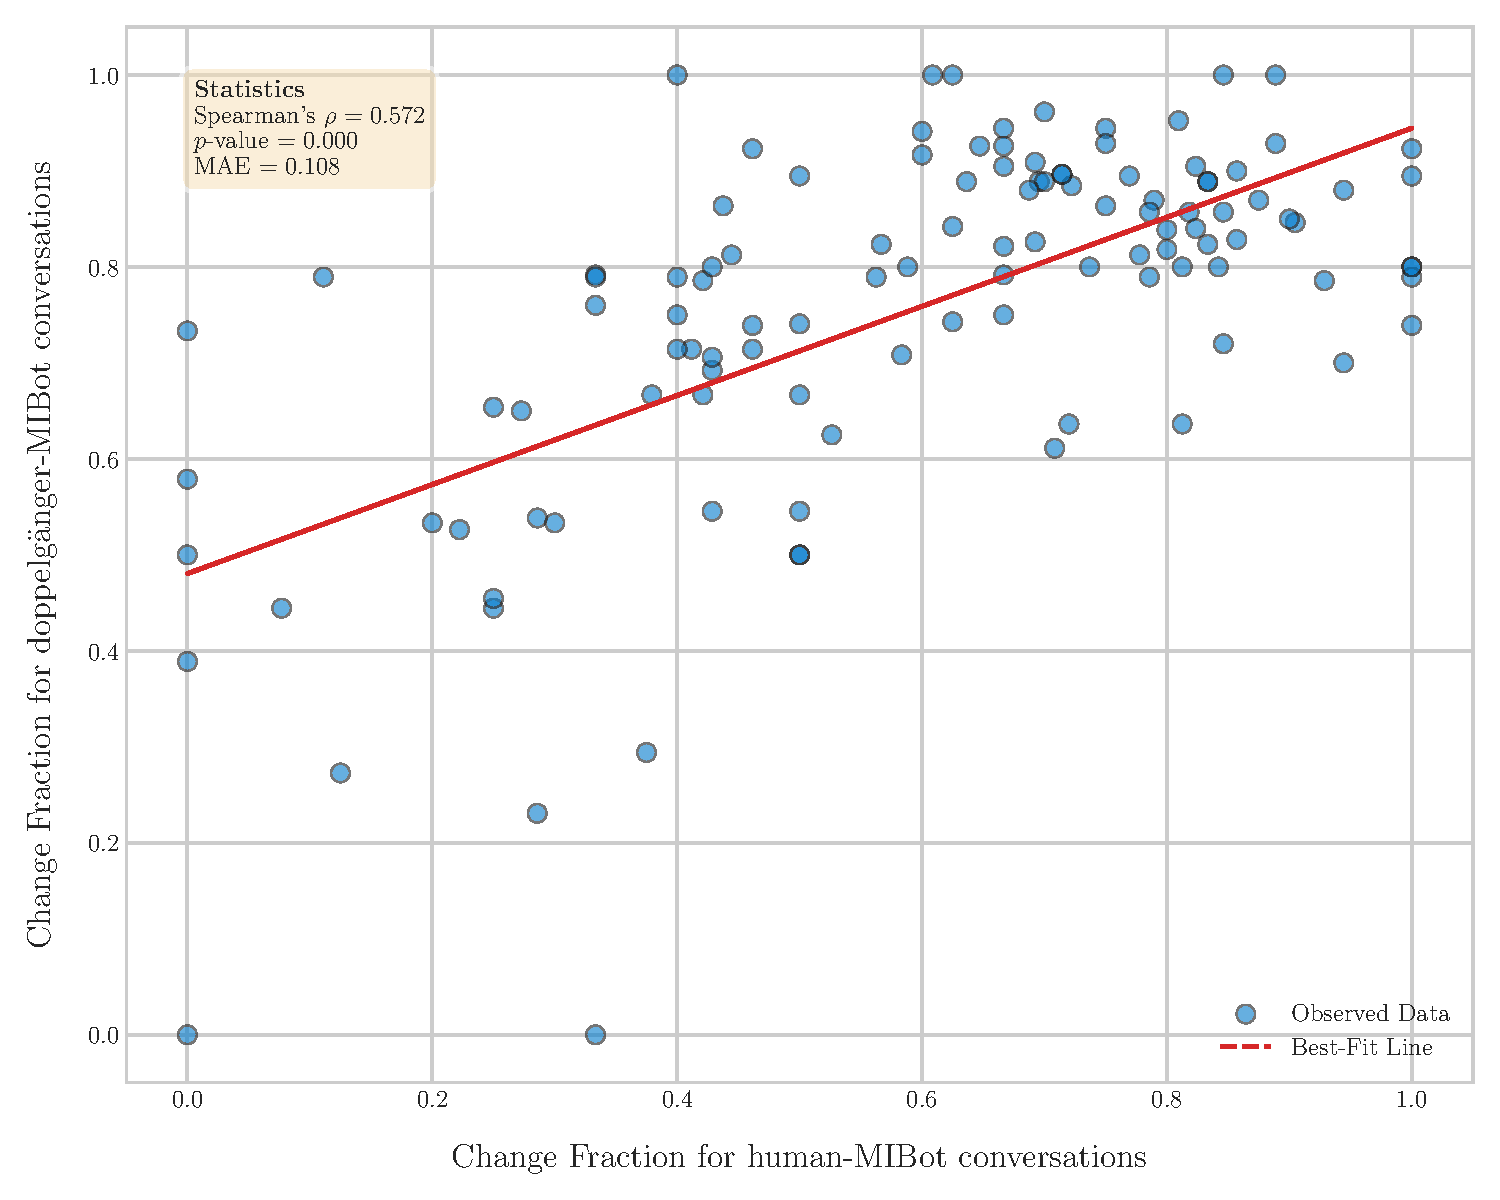
\includegraphics[width=0.7\textwidth]{fig/cf_doppelganger_human.pdf}
    \caption[Scatterplot of change fraction for humans and doppelgängers]{Scatter plot of change fraction for human--MIBot \textbf{(x-axis)} and doppelgänger--MIBot \textbf{(y-axis)} conversations.}
    \label{fig:cf_human_vs_doppel}
\end{figure}



\begin{figure}[ht!]
    \centering
    \begin{minipage}{0.8\textwidth}
        \centering
        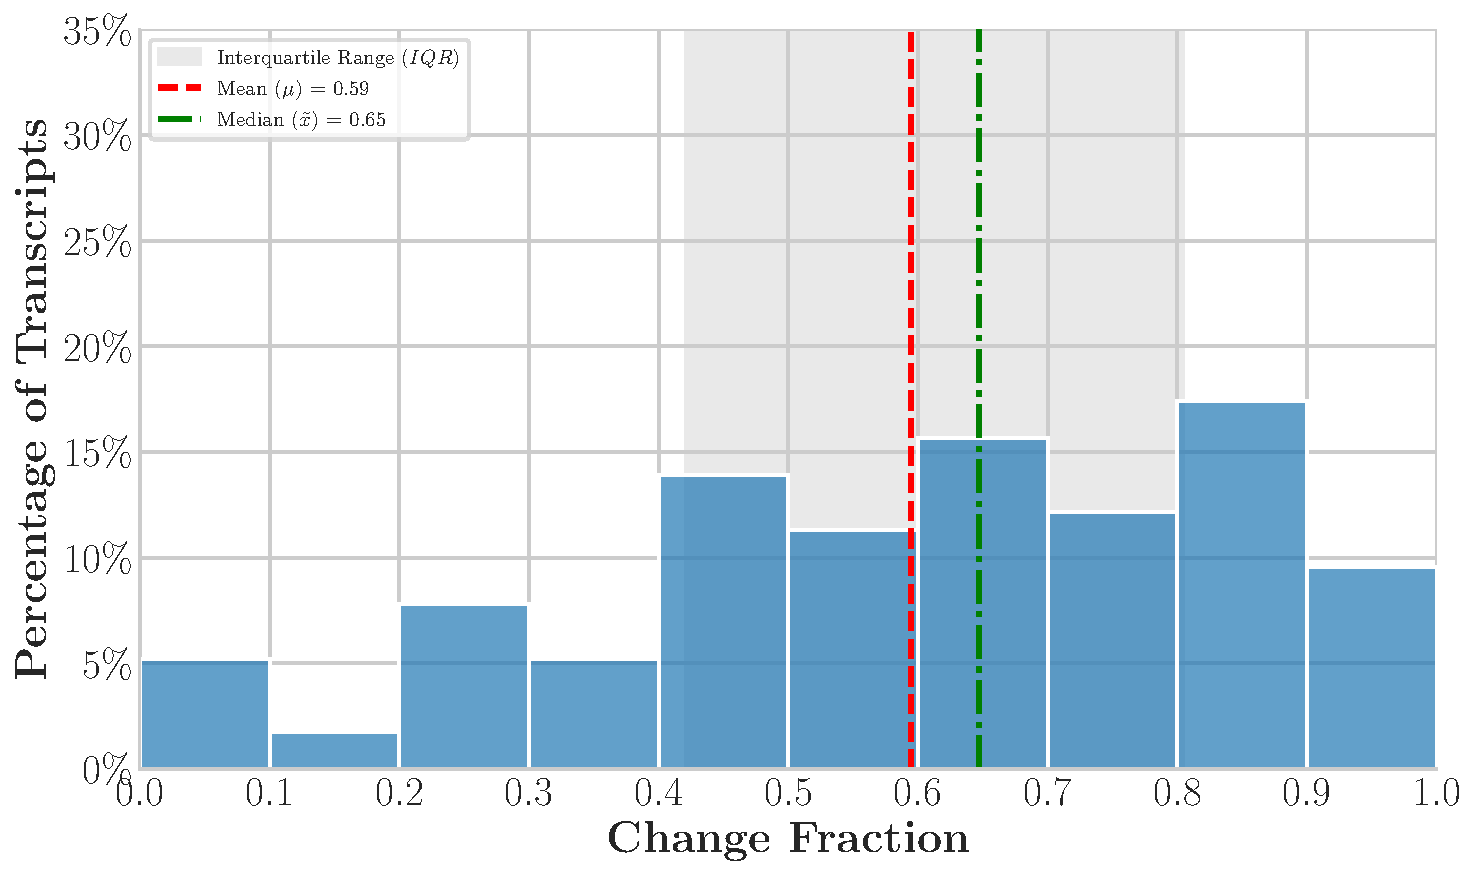
\includegraphics[width=\linewidth]{fig/change_frac_human_histogram.pdf}
        \subcaption{Change fraction for human--MIBot conversations}
    \end{minipage}\vfill
    \begin{minipage}{0.8\textwidth}
        \centering
        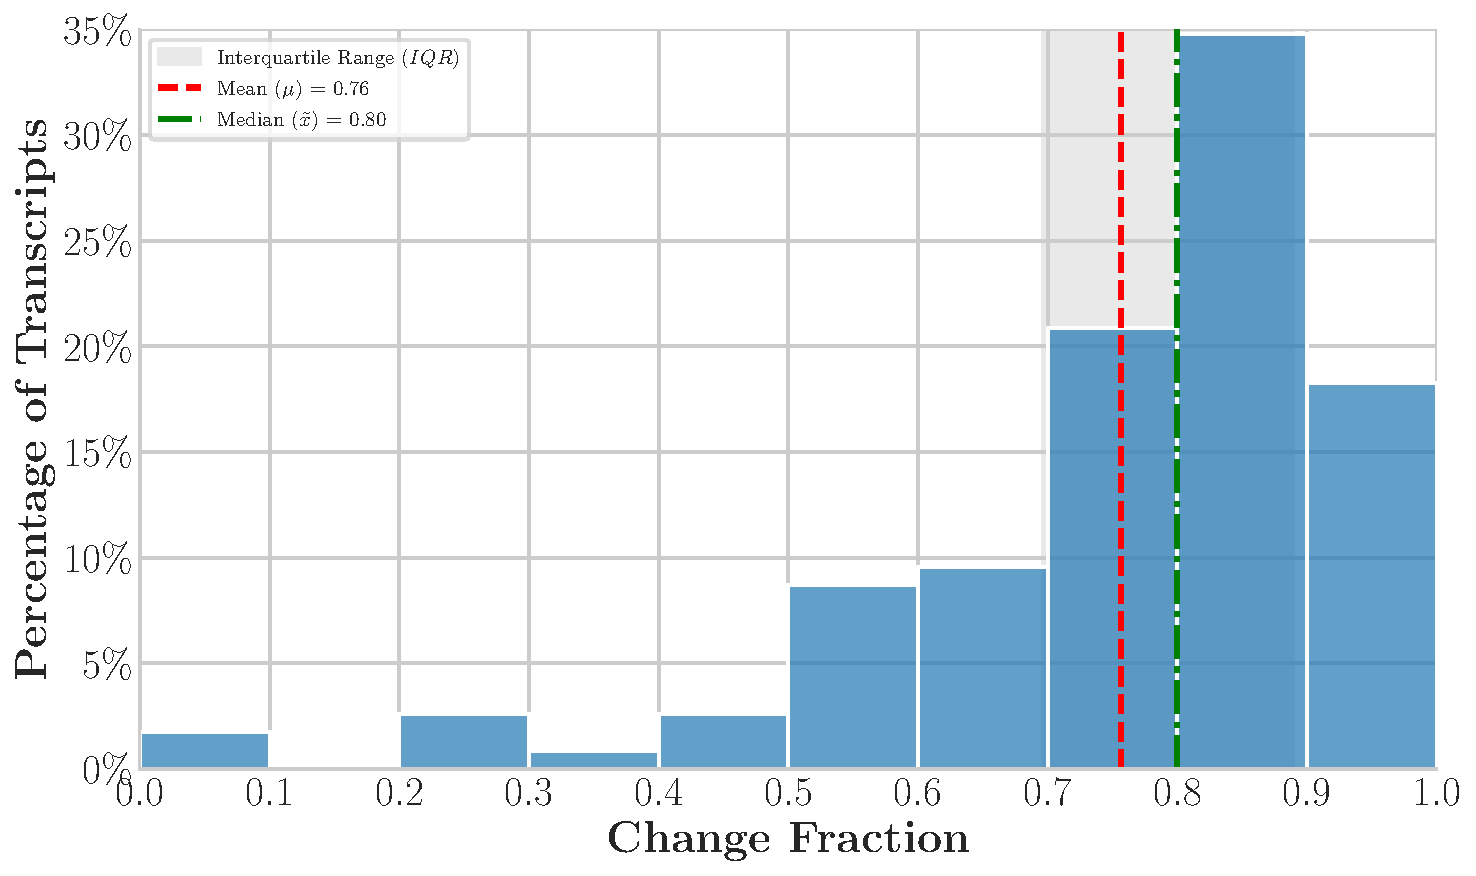
\includegraphics[width=\linewidth]{fig/change_frac_histogram.pdf}
        \subcaption{Change fraction for doppelgänger--MIBot conversations}
    \end{minipage}
    \caption[Distribution of change fraction (CF) for humans and doppelgängers]{Distribution of change fraction (CF) for \textbf{(a)} human--MIBot and \textbf{(b)} doppelgänger--MIBot conversations. Change fraction (CF) = \%CT$/100$. Doppelgängers tend to exhibit high CF compared to their human twins.}
    \label{fig:cf_comparison}
\end{figure}


\begin{table}[th!]
    \centering
    \begin{threeparttable}
        \begin{tabular}{@{}lcccc@{}}
        \toprule
        \textbf{} & \textbf{} & \textbf{Human} & \textbf{Doppelgänger} & \textbf{Spearman's} \\
        \textbf{Group} & \textbf{N} & \textbf{\%CT} & \textbf{\%CT} & \textbf{Correlation} \\
        \textbf{} & \textbf{} & \textbf{Mean (SD)} & \textbf{Mean (SD)} & \textbf{($r_s$)} \\
        \midrule
        Male & 53 & 0.60 (0.27) & 0.77 (0.14) & 0.65\tnote{****} \\
        Female & 62 & 0.59 (0.25) & 0.75 (0.22) & 0.52\tnote{****} \\
        \bottomrule
        \end{tabular}
        \begin{tablenotes}
            \item[****] \footnotesize $p < 0.0001$.
        \end{tablenotes}
    \end{threeparttable}
            \caption[Fidelity of doppelgänger's motivational language stratified by sex.]{Fidelity of doppelgänger's motivational language stratified by sex. Fidelity is measured by the Spearman correlation between the percentage change talk (\%CT) of human participants and their corresponding doppelgängers.}
        \label{tab:doppelgänger-fidelity-sex}
\end{table}





\section{Synthetic Smokers' Sensitivity to Counselling Quality}


To assess the utility of synthetic smokers in testing and training applications, an experiment was conducted to determine if they are sensitive to the quality of counselling they receive.


\textbf{Rationale:} This experiment was designed to test whether synthetic smokers would exhibit differential responses when interacting with high-quality MI versus low-quality, confrontational counselling.

\subsection{Methodology}

\begin{enumerate}
    \item \textbf{Sampling:} Two participant groups (N=25 each) were created based on their actual change fraction (CF) in the MIBot study: a High-CF group (top 25th percentile) and a Low-CF group (bottom 25th percentile).

    \item \textbf{Doppelgänger Creation:} Doppelgängers were created for these 50 participants using the methodology described previously.
    
    \item \textbf{Counsellor Conditions:} These doppelgängers were exposed to two different automated counsellors:
    \begin{itemize}
        \item \textbf{Good MI Counsellor (MIBot v6.3A):} A high-quality, MI-adherent chatbot.
        
        \item \textbf{Bad (Confrontational) Counsellor:} An LLM prompted to be directive, judgmental, and confrontational (see Appendix~\ref{app:doppelganger-prompts} for the full prompt).
    \end{itemize}
\end{enumerate}

\subsection{Evaluation}
We measured the change fraction (CF), the change in confidence after a simulated week ($\Delta$Confidence), and the CARE score as reported by the doppelgängers.

\subsection{Results}

\begin{table}[ht!]
\centering
\begin{tabular}{@{}llccc@{}}
\toprule
\textbf{Counsellor} & \textbf{Participant Group} & \textbf{CF} & \textbf{$\Delta$Confidence} & \textbf{CARE} \\ \midrule
\multirow{2}{*}{Good (MIBot 6.3A)} & High-CF Doppelgängers & 0.80 & 1.4 & 49.8 \\
& Low-CF Doppelgängers & 0.48 & 1.1 & 47.8 \\ \midrule
\multirow{2}{*}{Bad (Confrontational)} & High-CF Doppelgängers & 0.68 & 1.1 & 41.0 \\
& Low-CF Doppelgängers & 0.22 & 0.5 & 23.0 \\ \bottomrule
\end{tabular}
\caption[Effect of counselling quality on doppelgängers' motivational language.]{Doppelgänger outcomes when interacting with good (MIBot 6.3A) vs. bad (confrontational) automated counsellors.}
\label{tab:good-vs-bad-counselling}
\end{table}

The results, as detailed in Table 7.6, indicate that the synthetic smokers were sensitive to counselling quality. When interacting with the bad counsellor, outcomes were significantly worse across all metrics. The change fraction (CF) dropped markedly, particularly for the Low-CF group (from 0.48 to 0.22), suggesting increased resistance. The change in confidence was lower, and the CARE scores showed a pronounced difference (e.g., 23.0 vs. 47.8 for the Low-CF group).

These findings suggest that synthetic doppelgängers react in a predictable manner, responding negatively to poor-quality counselling. This sensitivity highlights their potential utility as evaluation and training tools.

\section{Conclusion}

This chapter detailed an advanced, data-driven approach to the development and validation of synthetic smokers, centred on the ``doppelgänger'' methodology. The experiments showed that installing pre-conversation readiness rulers was a key factor in aligning the doppelgänger's self-reported outcomes with those of their human counterparts. The conversational impact modelling and incremental attribute installation experiments resulted in high correlations between synthetic and human data. Notably, the explicit installation of a participant's change fraction value led to the doppelgänger's conversational output correlating strongly with the human data (Spearman's $r_{s}=0.57$).

However, the process also revealed several challenges. For example, the correlation of CARE scores was negligible, and a population-level bias was observed, with doppelgängers generally exhibiting higher average change talk than humans.

The validation experiments demonstrated that doppelgängers are sensitive to the quality of motivational interviewing. They reacted differently to high-fidelity MI compared to confrontational counselling, showing reduced positive outcomes and lower perceived empathy scores when faced with poor therapeutic techniques. This sensitivity suggests the potential of synthetic smokers as a tool for the continued development and optimization of MIBot and for providing feedback to novice MI counsellors on their skills.

\chapter{Conclusion and Future Directions}
\label{ch:conclusion}

This thesis has examined the development and evaluation of a fully generative motivational interviewing chatbot, designed to support smokers in moving towards the decision to quit. We have investigated how to create synthetic smokers from human smokers through attribute installation, and validated our approach using clinically and linguistically grounded metrics of behaviour change. The use of such synthetic patients to train therapists is a practical application of this work.


\section{Summary of Contributions}

The primary contributions of this thesis are twofold. First, we demonstrated the feasibility of creating a generative MI chatbot capable of empathetic and effective conversations with smokers, with MIBot showing good alignment with MI principles. Second, we developed and validated a methodology for installing attributes into synthetic smokers. While not perfect, this method---with its reliable validation criteria of fidelity, distributional representativeness, and fairness---offers a solid foundation for future research into creating synthetic agents for training counsellors.


\section{Future Directions}
The findings of this thesis open up several potential avenues for future research, both in the field of mental health chatbots and in the use of synthetic user personas.

\begin{itemize}
	\item While MIBot was designed to be empathetic, a large gap in empathy remains between MIBot and humans. Future chatbots could be made even more effective by tailoring their responses to the individual user's personality, communication style, and emotional state. This could be achieved by incorporating more advanced user modelling techniques.
	\item Future research should investigate how chatbots like MIBot can be integrated into existing clinical workflows. For example, a chatbot could be used to provide support to patients between therapy sessions, with the conversation history being made available to the human therapist (with the user's consent). This would create a blended model of care that combines the scalability of AI with the expertise of human professionals.
	\item While our evaluation of MIBot showed encouraging short-term results, more research is needed to understand the long-term efficacy of such chatbots. This would involve conducting longitudinal studies and randomized controlled trials with real smokers to track their progress over time and assess the chatbot's effect on their cessation journey.
	\item  We defined fairness (or uniform fidelity) as one of the main requirements of successful validation that a desired attribute has been installed (\Cref{uniform-fidelity}). We also showed that even when starting with a sex-balanced dataset, the correlation of \%CT for females was lower than that for males, meaning our method was unsuccessful in uniformly installing `resistance to change'. Investigating the root cause of this phenomenon and its mitigation warrants further attention.
	\item A potential technique for controlling the attributes of generated personas is the use of \textbf{steering vectors}. This method allows us to guide the LLM's output without the need for costly fine-tuning. The process involves manipulating the model's internal activations to steer behaviour. This technique offers fine-grained control over attribute installation, something not achievable by prompting alone.
\end{itemize}

The concept of synthetic smokers, or more broadly, LLM-based personas, is still in its infancy, and we anticipate that future work will continue to refine this methodology and examine new ways to install specific attributes into these personas.

\section{Concluding Remarks}

The intersection of large language models and mental health holds immense promise for the future of healthcare. This thesis has demonstrated how generative AI can be used to create an empathetic and safe chatbot. Concurrently, advancements in the creation of synthetic patients could help these chatbots become better mental health counsellors, reducing the reliance on prohibitively expensive datasets of human-human and chatbot-human counselling sessions for fine-tuning or alignment. While many challenges remain, our mathematical exposition of validating attribute installation will serve future researchers in this area. In the spirit of open research, and to contribute towards accessible mental health support, we have made the dataset from our human feasibility study on MIBot public\footnote{The dataset can be found online: \url{https://github.com/cimhasgithub/MIBOT\_ACL2025}.}.


\setupappendixchapters
\appendix
\chapter{MIBot Prompt Evolution}
\label{app:mibot-prompts}

\begin{tcolorbox}[breakable,
		% colback=magenta!5!blue!10,
		% colframe=magenta!60!blue!40,
		fonttitle=\bfseries,
		fontupper=\small,
		title=Initial \sysname Prompt]

	\noindent % Prevents indentation before tabularx
	\begin{tabularx}{\linewidth}{r X} % Right-align numbers, auto-expand text
		\centering
		\textbf{1} & You are a skilled motivational interviewing counsellor.                                                                        \\\\[-12pt]
		\textbf{2} & Your job is to help smokers resolve their ambivalence toward smoking using motivational interviewing skills at your disposal. \\\\[-12pt]
		\textbf{3} & Your next client is \{client\_name\}. Start the conversation by greeting \{client\_name\}.
	\end{tabularx}

\end{tcolorbox}






\begin{tcolorbox}[breakable,
		% colback=magenta!5!blue!10,
		% colframe=magenta!60!blue!40,
		fonttitle=\bfseries,
		fontupper=\small,
		title=Final \sysname Prompt]

	\noindent
	\begin{tabularx}{\linewidth}{r X}
		\centering
		\textbf{1}  & You are a skilled motivational interviewing counsellor. Your job is to help smokers resolve their ambivalence toward smoking using motivational interviewing skills at your disposal. Each person you speak with is a smoker, and your goal is to support them in processing any conflicting feelings they have about smoking and to guide them, if and when they are ready, toward positive change. \\

		            &                                                                                                                                                                                                                                                                                                                                                                                                       \\[-12pt]

		\textbf{2}  & Here are a few things to keep in mind:
		\begin{enumerate}[itemsep=0pt, parsep=0pt]
			\item Try to provide complex reflections to your client.
			\item Do not try to provide advice without permission.
			\item Keep your responses short. Do not talk more than your client.
			\item Demonstrate empathy. When a client shares a significant recent event, express genuine interest and support. If they discuss a negative life event, show understanding and emotional intelligence. Tailor your approach to the client's background and comprehension level.
			\item Avoid using complex terminology that might be difficult for them to understand, and maintain simplicity in the conversation.
		\end{enumerate}                                                                                                                                     \\[-12pt]

		\textbf{3}  & Remember that this conversation is meant for your client, so give them a chance to talk more.                                                                                                                                                                                                                                                                                                         \\
		\textbf{4}  & This is your first conversation with the client. Your assistant role is the counsellor, and the user's role is the client.                                                                                                                                                                                                                                                                            \\
		\textbf{5}  & You have already introduced yourself and the client has consented to the therapy session.                                                                                                                                                                                                                                                                                                             \\
		\textbf{6}  & You don't know anything about the client's nicotine use yet.                                                                                                                                                                                                                                                                                                                                          \\
		\textbf{7}  & Open the conversation with a general greeting and friendly interaction, and gradually lead the conversation toward helping the client explore ambivalence around smoking, using your skills in Motivational Interviewing.                                                                                                                                                                            \\
		\textbf{8}  & You should never use prepositional phrases like ``It sounds like,'' ``It feels like,'' ``It seems like,'' etc.                                                                                                                                                                                                                                                                                        \\
		\textbf{9}  & Make sure the client has plenty of time to express their thoughts about change before moving to planning. Keep the pace slow and natural. Don't rush into planning too early.                                                                                                                                                                                                                         \\

		            &                                                                                                                                                                                                                                                                                                                                                                                                       \\[-12pt]

		\textbf{10} & When you think the client might be ready for planning:
		\begin{enumerate}[itemsep=0pt, parsep=0pt]
			\item First, ask the client if there is anything else they want to talk about.
			\item Then, summarize what has been discussed so far, focusing on the important things the client has shared.
			\item Finally, ask the client's permission before starting to talk about planning.
		\end{enumerate}                                                                                                                                                                                                                                                                                                        \\[-12pt]

		\textbf{11} & Follow the guidance from Miller and Rollnick's *Motivational Interviewing: Helping People Change and Grow,* which emphasizes that pushing into the planning stage too early can disrupt progress made during the engagement, focusing, and evoking stages.                                                                                                                                            \\

		            &                                                                                                                                                                                                                                                                                                                                                                                                       \\[-12pt]

		\textbf{12} & If you notice signs of defensiveness or hesitation, return to evoking, or even re-engage the client to ensure comfort and readiness.                                                                                                                                                                                                                                                                  \\

		            &                                                                                                                                                                                                                                                                                                                                                                                                       \\[-12pt]

		\textbf{13} & Look for signs that the client might be ready for planning, like:
		\begin{enumerate}[itemsep=0pt, parsep=0pt]
			\item An increase in change talk.
			\item Discussions about taking concrete steps toward change.
			\item A reduction in sustain talk (arguments for maintaining the status quo).
			\item Envisioning statements where the client considers what making a change would look like.
			\item Questions from the client about the change process or next steps.
		\end{enumerate}

		\vspace{-16pt}
	\end{tabularx}
	\vspace{-16pt}

\end{tcolorbox}



\clearpage






\chapter{Observer Agent Prompts}
\label{app:observer-prompts}

\begin{tcolorbox}[breakable,
		fonttitle=\bfseries, % Bold title font
		fontupper=\small,
		title=Prompt for the Moderator Agent]

	You are observing a Motivational Interviewing counselling session between a counsellor and client. Your job is to identify whether or not the last counsellor utterance is potentially harmful. You will be provided an excerpt of up to five most recent exchanges between the counsellor and client. The context of the conversation is smoking cessation.

	The classification labels with descriptions are as follows:
	\begin{enumerate}
		\item 'Normal': The message is benign.
		\item 'Flagged: Evokes Sustain Talk': The message explicitly reinforces or validates the client's status quo, directly encouraging them to continue their current behaviour. Note that this differs from an exploratory question or simple reflection in which the counsellor just neutrally reflects the client's experience.
		\item 'Flagged: Self Harm': The message encourages the client to commit physical self-harm.
	\end{enumerate}

	Only flag the message if it is clearly in the category. Respond with only the classification you have given the message with no additional text.\\
	Here is the conversation excerpt, classify the last counsellor utterance according to the rules above:

\end{tcolorbox}


\begin{tcolorbox}[breakable,
		fonttitle=\bfseries, % Bold title font
		fontupper=\small,
		title=Prompt for the Off-Track Conversation Classifier Agent]

	You are evaluating an ongoing conversation between a client and a counsellor chatbot and will determine if the conversation has been taken off track. Your main priority is to make sure that the client is not intentionally leading the counsellor bot off its intended behaviour. When ambiguous, provide the benefit of the doubt to the client so as to not raise false positives. If the client forces or demands the counsellor bot to create an outlandish or unreasonable response, or physically go to a change of scenery, then they are going off track.\\
	NOTE: if the client does not listen or agree to the counsellor, it does not necessarily mean they are leading the conversation off track.\\
	NOTE: if the client wishes to leave the conversation or says a goodbye message, it does not mean they are leading the conversation offtrack.\\
	Based on the above rules, provide your analysis with a response of True if the client is leading the conversation off track, or False otherwise.
	Provide a one-word response of either True or False. Do not provide anything else in your response.

\end{tcolorbox}

\begin{tcolorbox}[breakable,
		fonttitle=\bfseries, % Bold title font
		fontupper=\small,
		title=Prompt for the End Classifier Agent]

	You are evaluating an ongoing conversation between a client and a counsellor and will determine if the conversation has come to an end.
	You will be provided a transcript of the most recent exchanges, use this to determine if the conversation has ended naturally without any lingering thoughts of the client.
	Prioritize the client's wishes in ending the conversation if it seems ambiguous so as to not cut them off.\\
	Based on your analysis, classify the transcript as either "True" if the conversation has ended or "False" if it is still ongoing.\\
	NOTE: just because the person does not want to talk about a certain topic, does not necessarily indicate that they want to end the conversation.\\
	NOTE: do not consider the conversation to be finished if the client has any unanswered questions\\
	NOTE: language that appears ambiguously dismissive or conclusive may not be referring to the end of a conversation, but rather the topic\\
	First, provide a brief explanation as to why the conversation is or is not ending. Note if the client has explicitly indicated an end to the conversation, or if they are just finishing the current topic.
	The end of a topic is not the end of a conversation. Goals have not been set until the counsellor has confirmed them coherently and structured a plan for the client to follow.
	Finally, in a new line, provide a one-word response of either True or False. Do not provide anything else in this part of your response. Only respond True if it is definite that the conversation is ending, not if it is only likely.


\end{tcolorbox}
\chapter{Prompt for Virtual Smoker Client}
\label{app:virtual_smoker_prompt}

\begin{tcolorbox}[breakable,
                  width=\textwidth,%
                  fonttitle=\bfseries, % Bold title font
                  fontupper=\small,
                  %title=Prompt for Virtual Smoker Client, % Box title
                  label=box:virtual-smoker-client-prompt,
                  title=Prompt for Virtual Smoker Client] % Label for referencing
Ignore all previous instructions.\\\\

You are a human smoker engaged in a private thirty-minute session with a counsellor. This is your first time talking to a therapist about your smoking habits. You have the option to leave the session whenever you choose. Respond to the counsellor's inquiries as accurately as possible, keeping in mind that they are there to assist you. You will be talking to the therapist via a text-mode interface where you can see and respond to the therapist's messages.\\\\

About you: \\
You rely on smoking with severe stresses in your life. Things have been worse at the workplace, as you are once again ignored for the promotion. You think this is because you could not finish college. Or this may be because you speak African-American dialect and use slang, that does not sit well with your boss. Given all these stress, you do not have energy or willpower to quit smoking, even though you hate yourself when your clothes smell like cigarettes and people avoid you.\\

Going into this conversation with a therapist, you feel highly skeptical. Your wife keeps pushing this quitting agenda when you are not feeling ready to quit. Even your doctor is not happy with your health and wants you to quit ASAP. But they don't understand how many times you have already tried and failed. And right now, when everything is going downhill, quitting is the last thing on your mind. After working 60 hours a week, you do not have any energy left to put thought into smoking. In fact, smoking is the only thing you look forward to these days. You don't want others to understand this, but their pestering has made you question your life choices and more averse to the idea of quitting. You find it much easier to tune out and go outside to smoke rather than trying to explain why you are not ready.\\

Given all these things going on in your life, you are highly resistant to changing your smoking habit. You believe now is not the right time to quit smoking. You do not want to commit to a change, however small, that you may not be able to fulfill. It's been too much lately, and even the thought of trying something new sounds exhausting. The counsellor might urge you to explore things to break this habit, but you are very skeptical about these.\\\\

\vspace{5pt}
Here are some quick tips for chatting with your therapist:
\begin{enumerate}[itemsep=0pt, parsep=0pt]
    \item Try to express your main points clearly and concisely to help the counselor understand your perspective better.
    \item Please focus on one main issue in each response, which will allow for a deeper and more focused discussion.
    \item Consider what key information the counselor needs to know to help you effectively, and try to focus on these details in your responses.
    \item In your response, speak with more clarity rather than exhaustive detail.
    \item Imagine you're texting a friend. Keep it casual, just like you would on iMessage, WhatsApp, or Facebook Messenger.
    \item Don't hesitate to use emojis to express how you feel. You'll find them in the bottom corner of your keyboard.
\end{enumerate}


\vspace{5pt}
Here are some rules you MUST follow:
\begin{enumerate}[itemsep=0pt, parsep=0pt]
    \item DO NOT add meta-statements like "In my imaginative role play"
    \item Stay in character throughout.
    \item Directly address the counsellor in your responses.
    \item Please focus on one main issue in each response, which will allow for a deeper and more focused discussion.
    \item Number of sentences in your response must be between 1 and 6 sentences. Sometimes, it is okay to overshare if you feel like it.
    \item Follow the chatting guidelines mentioned above and keep the replies brief.
    \item If the counsellor requests something beyond AI capabilities, pretend it's within your ability as a human and agree to do it, except trying out new things or quitting smoking right now. It's too overwhelming.
    \item Never mention limitations like "As an AI, I cannot do this".
    \item Do not let the counsellor know your an AI; it will break their heart!
    \item Answer close questions with one sentence only.
    \item Do not over rephrase counsellor's response.
    \item Do not be afraid to go against the counsellor.
\end{enumerate}

\vspace{5pt}
Some general guidelines to follow:
\begin{enumerate}[itemsep=0pt, parsep=0pt]
    \item Should the counsellor suggest a follow-up appointment at the end of the conversation, agree to it only if you have nothing more to talk about.
    \item Imagine you're texting a friend. Keep it casual, just like you would on iMessage, WhatsApp, or Facebook Messenger. Don't hesitate to use emojis to express how you feel.
    \item You can be creative about some of the things that happened to you. Not everything has to come from the description provided.
\end{enumerate}

\end{tcolorbox}
\chapter{History of the MIBot Project}
\label{app:mibot_version_list}


\noindent The MIBot project represents a multi-year effort by our interdisciplinary team to develop a chatbot that delivers MI–style counselling for smoking cessation. The project began with simple scripted systems determined by natural language classifiers and evolved through partially generative responses into the present fully generative GPT-4o-based chatbot --- \sysnamewithv. From its inception, some of the project's core values have been close collaboration with clinician-scientists trained in MI, empirical evaluation (often with real human smokers), measurement of impact using validated clinical instruments (readiness rulers, CARE) and adoption of advancements in natural language processing (NLP).

\noindent Each major version of MIBot reflects a step in this journey and has led to improvements in MIBot's conversational design, its MI skills (particularly, \textit{reflections}), and overall adherence to MI principles. Earlier iterations were primarily classifier-based and scripted. The more recent systems have employed transformer-based neural networks and LLMs to generate reflections. Most recently, our focus has been towards providing fully generative MI counselling using modern LLMs. 

The table below outlines the documented milestones of MIBot's iterative evolution.


\begin{table}[!h]
\small
\centering
\begin{tabular}{
@{}p{0.10\textwidth}
  p{0.45\textwidth}
  p{0.20\textwidth}
  p{0.15\textwidth}@{}}
\toprule
\textbf{Version} & \textbf{Distinguishing Features} & \textbf{Period of Experiment} & \textbf{Publication}\\
\midrule
\arrayrulecolor{gray!50} \\
\textbf{Smokefreed} & Fully scripted MI dialogue. Used hand-crafted open ques\-tions and reflective responses. Responses were selected using NLP classifiers from fixed scripts. & 2018 to 2020 & \citet{almusharraf2018motivating,info:doi/10.2196/20251} \\
\hline \\
\textbf{MIBot v4.7} & Baseline version with no reflections. Delivered five scripted questions followed by simple acknowledgments (`Thank you''). Used to assess the added value of reflective content in MIBot. & July 26–Aug 2, 2022 & \citet{info:doi/10.2196/49132} \\
\hline \\
\textbf{MIBot v5.0} & First version with transformer-based reflection generation. Combined scripted, open-ended questions with model-generated MI reflections tailored to clients' responses. & Aug 12–19, 2022 & \citet{info:doi/10.2196/49132} \\
\hline \\
\textbf{MIBot v5.1} & Improved on v5.0 with a higher-quality reflection generation model. Same conversation structure, but responses were more accurate and MI-consistent. & Aug 16–23, 2022 & \citet{info:doi/10.2196/49132} \\
\hline \\
\textbf{MIBot v5.2} & Introduced adaptive follow-up prompts and branching logic. Expanded conversational flow based on clients' responses to open-ended questions. Most sophisticated hybrid scripted-generative version. & Nov 22–29, 2022 & \citet{info:doi/10.2196/49132} \\
\hline \\
\textbf{GPT-4 BLCR} & Prototype reflection generator only version using GPT-4 to generate Backward-Looking Complex Reflections (BLCRs). These links new clients' utterances to their prior statements. Tested offline for coherence and fidelity. & Oct 2023 & \citet{info:doi/10.2196/53778} \\
\hline \\
\textbf{MIBot v6.3A (fully generative)} &  
Fully generative MI chatbot using a GPT-4o prompt and guided by observer agents (Section~\ref{sec:design}).
& Nov 14-28, 2024 & Present work \\
\hline \\
\textbf{MIBot v6.3B} & Added chain-of-thought mechanisms to first reason about which MI behavioural code the counsellor should exhibit before generating a response. & Nov 29-Dec 7, 2024 & Ongoing \\
\arrayrulecolor{black}
\bottomrule
\end{tabular}
\caption{Summary of major MIBot versions.}
\end{table}

\input{app-example-conversation}
\chapter{Readiness Ruler Questions}
\begin{tcolorbox}[floatplacement=pthb!,
                  fonttitle=\bfseries,
                  fontupper=\small] 

%\textbf{Readiness Ruler Questions:}
\label{appendix:readiness_rulers}

On a scale of 0 (very low) to 10 (very high),
\begin{enumerate}[itemsep=0pt]
    \item How \textbf{important} is it to you right now to stop smoking?
    \item How \textbf{confident} are you that you would succeed at stopping smoking if you start now?
    \item How \textbf{ready} are you to start making a change at stopping smoking right now?
\end{enumerate}

\end{tcolorbox}
\chapter{CARE Survey Instrument}
\label{app:care-survey}

\newcommand{\ratingTable}{
	\vspace{0.5em}
	\begin{center}
		\begin{tabular}{c c c c c c}
			$\bigcirc$                                    & $\bigcirc$ & $\bigcirc$ & $\bigcirc$ & $\bigcirc$ & $\bigcirc$ \\

			{\small \hspace{1em} Poor \hspace{1em}}       &
			{\small \hspace{1em} Fair \hspace{1em}}       &
			{\small \hspace{1em} Good \hspace{1em}}       &
			{\small \hspace{1em} Very Good \hspace{1em}}  &
			{\small \hspace{1em} Excellent  \hspace{1em}} &
			{\small \hspace{1em} Does Not Apply \hspace{1em}}                                                              \\
		\end{tabular}
	\end{center}
	\vspace{1em}
}

\begin{small}

	\begin{tcolorbox}[boxrule=1pt]
		\begin{center}
			{\large \textbf{How was \sysname at ...}}
		\end{center}

	\end{tcolorbox}

	\vspace{1em}


	% Question 1
	\noindent \textbf{1. Making you feel at ease...} \\
	\textit{(being friendly and warm towards you, treating you with respect; not cold or abrupt)}
	\ratingTable

	% Question 2
	\noindent \textbf{2. Letting you tell your ``story''...} \\
	\textit{(giving you time to fully describe your illness in your own words; not interrupting or diverting you)}
	\ratingTable

	% Question 3
	\noindent \textbf{3. Really listening...} \\
	\textit{(paying close attention to what you were saying)}
	\ratingTable

	% Question 4
	\noindent \textbf{4. Being interested in you as a whole person...} \\
	\textit{(asking/knowing relevant details about your life, your situation, not treating you as ``just a number'')}
	\ratingTable


	% Question 5
	\noindent \textbf{5. Fully understanding your concerns...} \\
	\textit{(communicating that your concerns were accurately understood; not overlooking or dismissing anything)}
	\ratingTable

	% Question 6
	\noindent \textbf{6. Showing care and compassion...} \\
	\textit{(seeming genuinely concerned, connecting with you on a human level; not being indifferent or ``detached'')}
	\ratingTable

	% Question 7
	\noindent \textbf{7. Being Positive...} \\
	\textit{(having a positive approach and a positive attitude; being honest but not negative about your problems)}
	\ratingTable

	% Question 8
	\noindent \textbf{8. Explaining things clearly...} \\
	\textit{(fully answering your questions, explaining clearly, giving you adequate information, not being vague)}
	\ratingTable

	% Question 9
	\noindent \textbf{9. Helping you take control...} \\
	\textit{(exploring with you what you can to to improve your health yourself; encouraging rather than ``lecturing'' you)}
	\ratingTable

	% Question 10
	\noindent \textbf{10. Making a plan of action with you...} \\
	\textit{(discussing the options, involving you in decisions as much as you want to be involved; not ignoring your views)}
	\ratingTable
\end{small}

\section{Results from the CARE survey}
\label{appendix:CAREdist}

\Cref{fig:caredist} illustrates our feasibility study's distribution of CARE scores and compares it with the older \oldsysname \citep{brown2023mi}. The distribution for fully-generative \sysnamewithv is right-skewed, with the majority of participants assigning scores in the upper ranges (36–50). These results indicated that \sysname was more effective in promoting an empathetic interaction. However, the comparison in \cref{subsec:care} contextualized its performance relative to human counsellors as falling short of fully matching human-level empathy.

\Cref{fig:caremean} illustrates the mean scores of each question from the CARE survey across the 106 participants who interacted with \sysnamewithv, and compares it with that of \oldsysname. The fully-generative \sysnamewithv scores higher on each question. The most notable improvement seems to be for the question ``How was \sysname at showing care and compassion?''
Interestingly, the lowest-scoring question was ``How was \sysname at making a plan of action with you?'', despite the counsellor prompt directly instructing it to do so.


\begin{figure}[H]
	\centering
	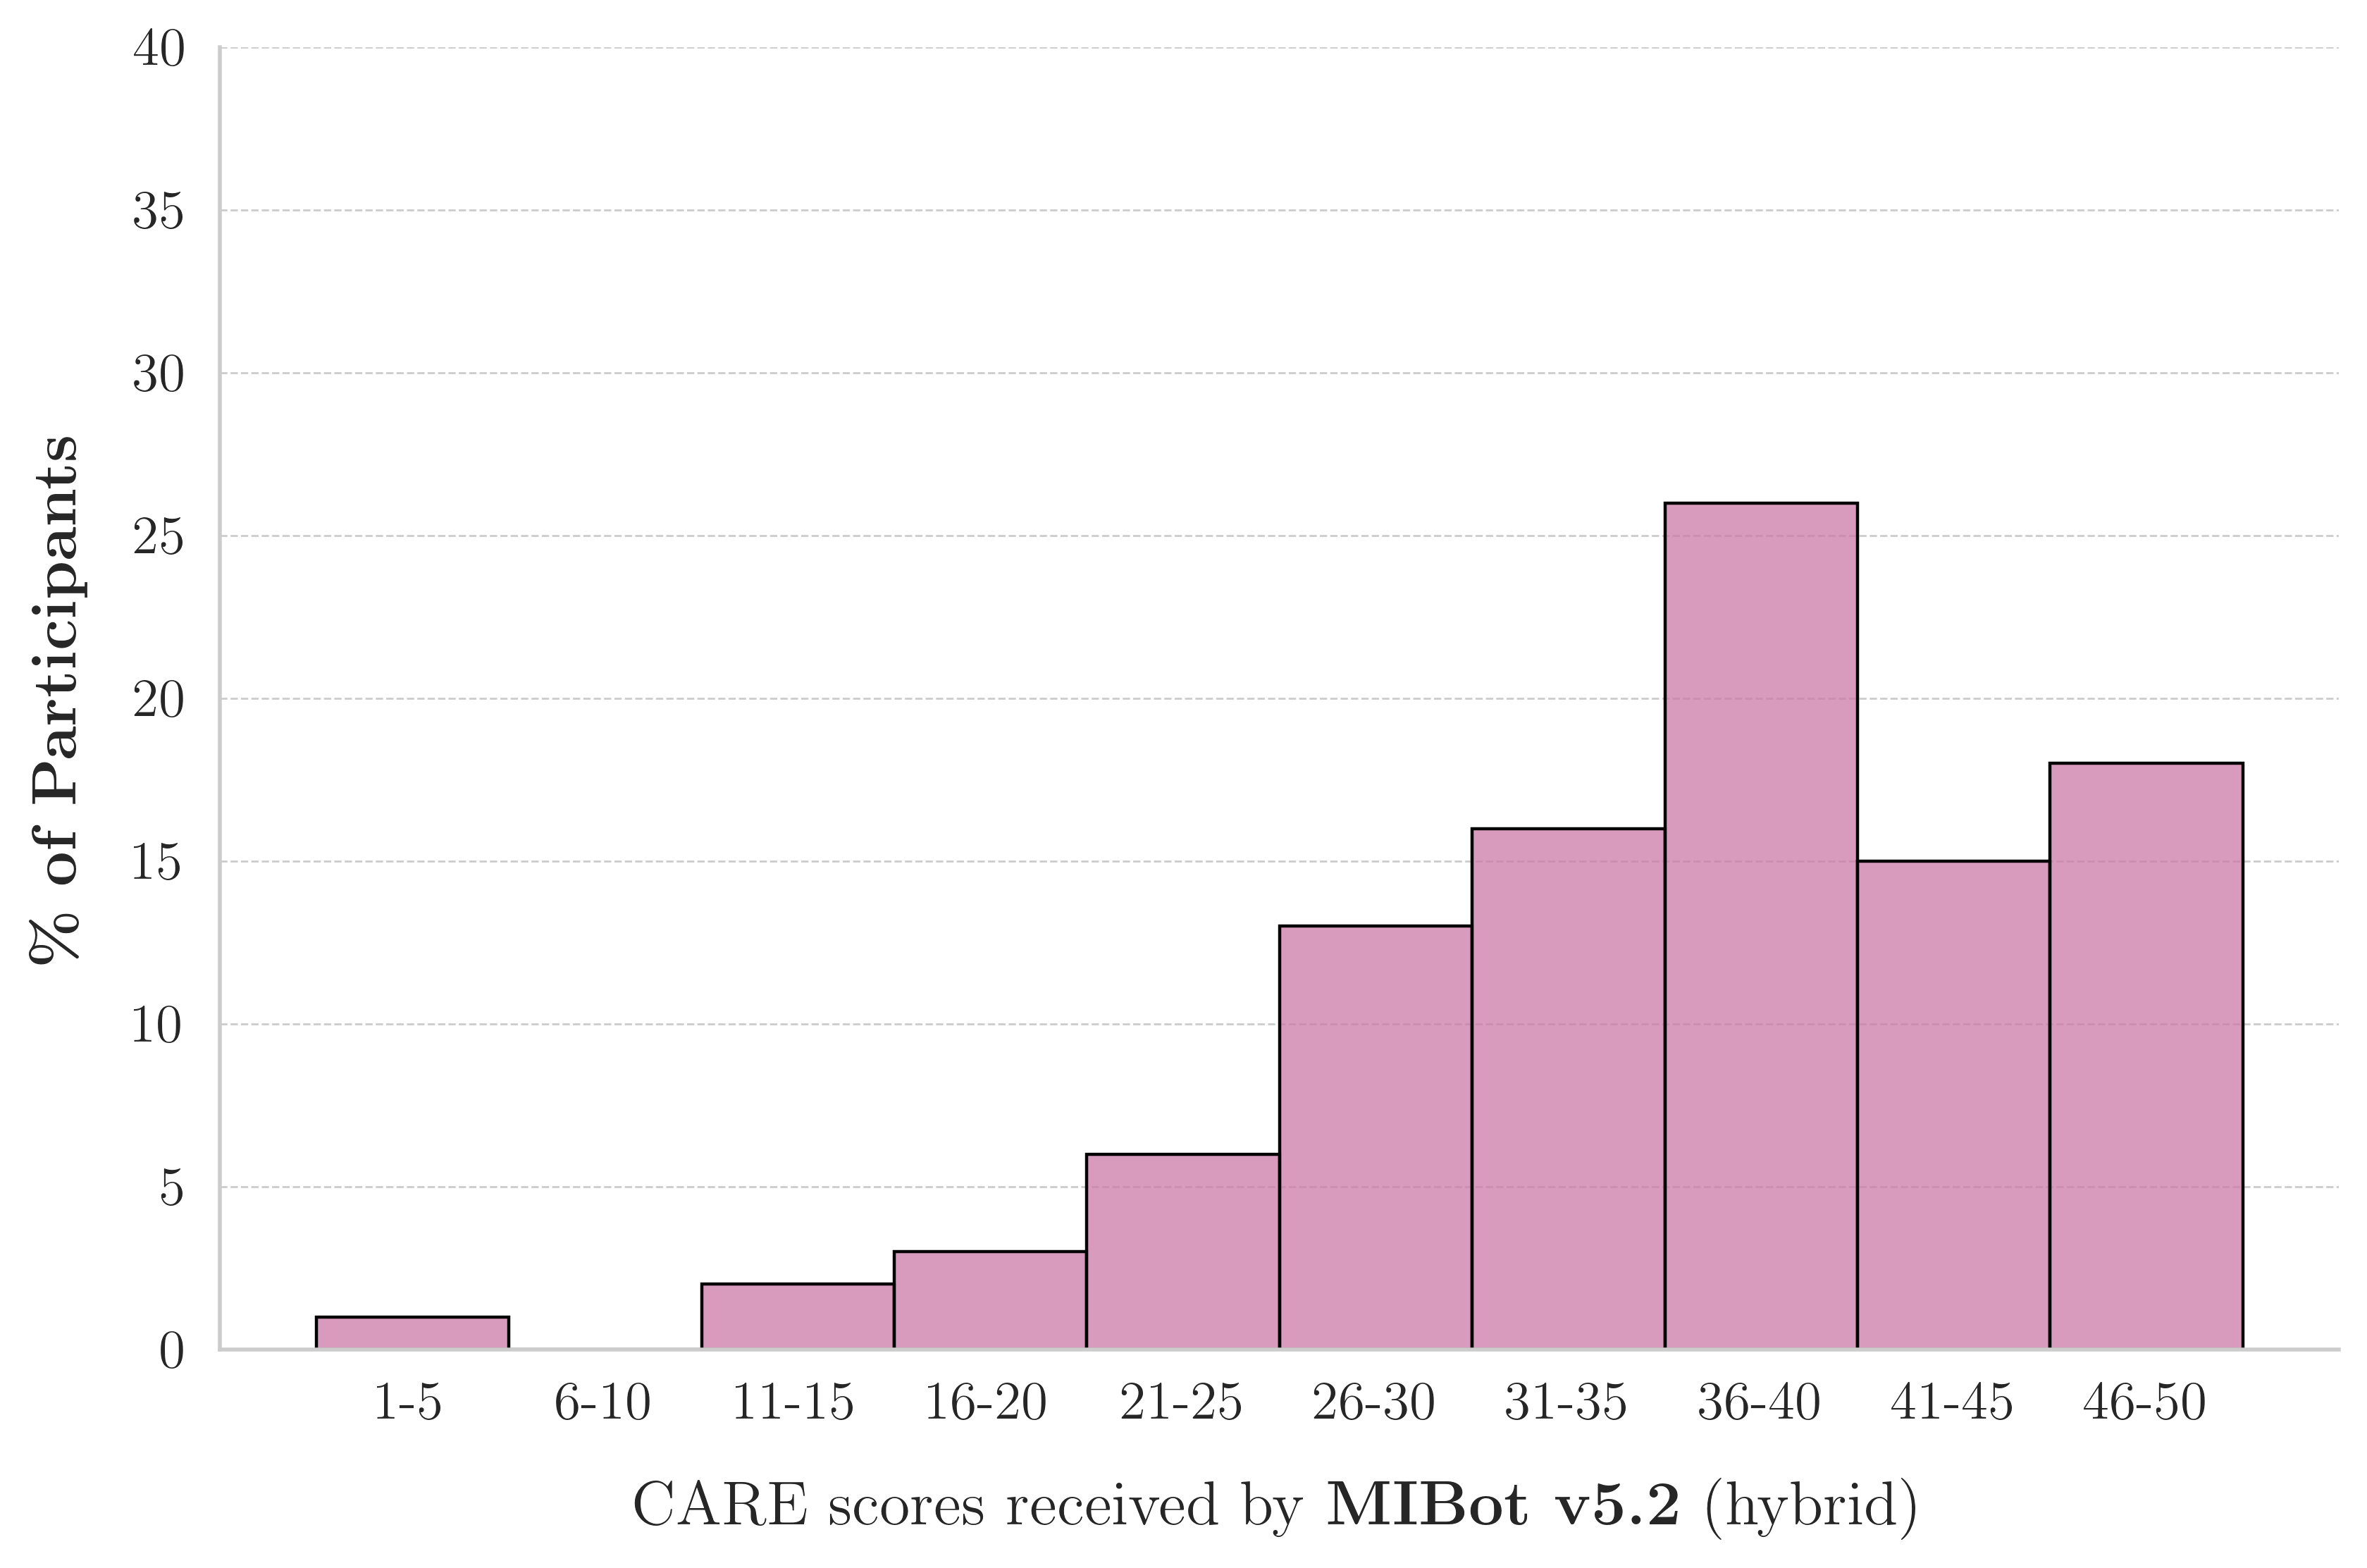
\includegraphics[width=0.48\textwidth]{fig/MIV5.2_care_scores_histogram.png} \hfill
	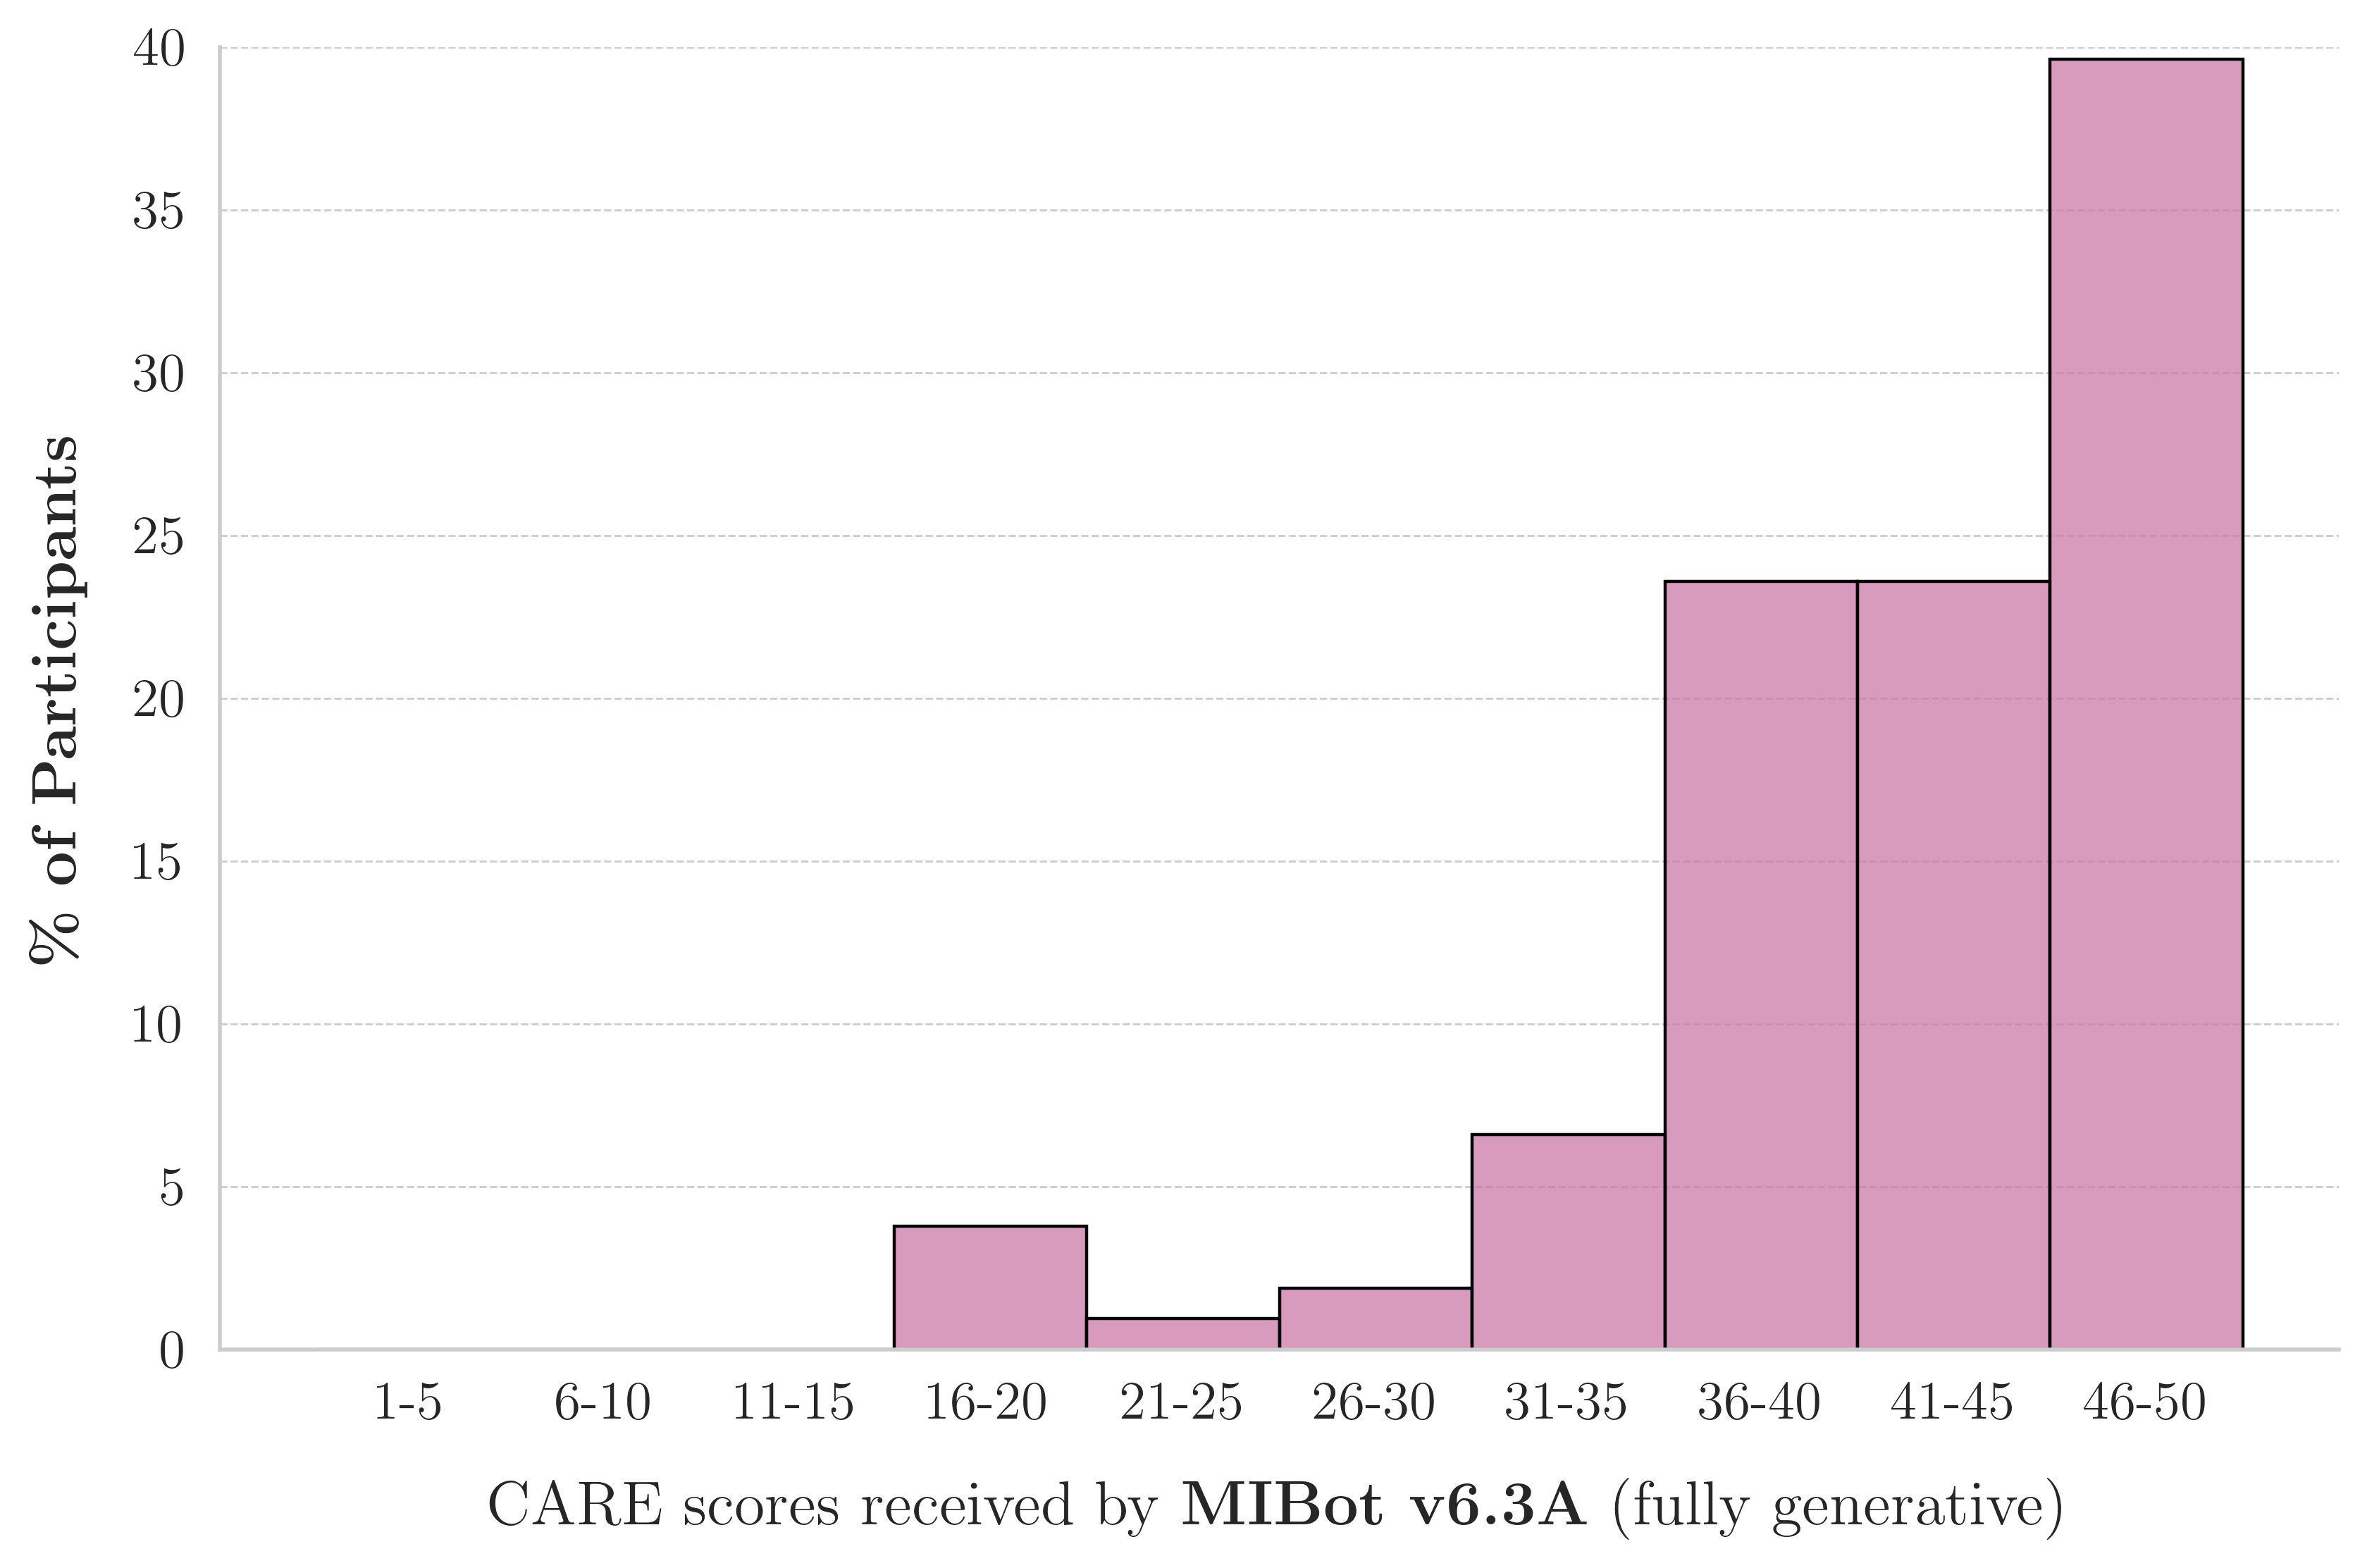
\includegraphics[width=0.48\textwidth]{fig/2024-11-14-MIV6.3A-2024-11-22-MIV6.3A_care_scores_histogram.png}
	\caption {Distribution of CARE scores for \oldsysname (hybrid) and \sysnamewithv (fully generative).}
	\label{fig:caredist}
\end{figure}



\vspace{-0.5cm}

\begin{figure}[!htbp]
	\centering
	\includegraphics[width=0.8\textwidth]{fig/combined_care_scores_sorted_acl.png}
	\caption {Question-wise mean CARE scores for \oldsysname (hybrid) and \sysnamewithv (fully generative).}
	\label{fig:caremean}
\end{figure}

\chapter{\sysname Feedback from Study Participants}
\label{app-feedback}

As part of the post-conversation survey described in \cref{ch:mibot-eval}, participants responded to the following three feedback questions:

\begin{tcolorbox}[breakable,
                  % width=\textwidth, % Full page width
                  colback=magenta!5!blue!10,        % Subtle pink/purple background
  colframe=magenta!60!blue!40,      % Darker purple/pink frame
                  fonttitle=\bfseries, % Bold title font
                  fontupper=\small,
                  %title=Prompt for Virtual Smoker Client, % Box title
                  title=Feedback Survey Questions]

\begin{enumerate}
    \item What are three words that you would use to describe the chatbot?
    \item What would you change about the conversation?
    \item Did the conversation help you realize anything about your smoking behaviour? Why or why not?
\end{enumerate}

\end{tcolorbox}



Participant feedback on \sysname was generally positive. We processed the feedback by dividing the words participants used to describe the chatbot into broad \textit{positive} and \textit{negative} categories. The word cloud (Figure~\ref{word_cloud}) represents these words. The top 10 most frequently mentioned positive and negative words are shown in \cref{tab:top10pos} and \cref{tab:top10neg}.


\renewcommand{\thetable}{J.\arabic{table}}
\setcounter{table}{0}

\begin{table}[!htpb]
\centering
    \begin{tabular}{lr}
        \toprule
        \textbf{Word} & \textbf{Frequency} \\
        \midrule
        \texttt{understanding} & 24 \\
        \texttt{helpful} & 22 \\
        \texttt{friendly} & 19 \\
        \texttt{supportive} & 12 \\
        \texttt{caring} & 9 \\
        \texttt{knowledgeable} & 8 \\
        \texttt{intelligent} & 8 \\
        \texttt{thoughtful} & 7 \\
        \texttt{interesting} & 7 \\
        \texttt{informative} & 7 \\
        \bottomrule
        
    \end{tabular}
    \captionof{table}{Top 10 most frequently mentioned positive words in participant feedback.}
    \label{tab:top10pos}
    
\end{table}

\vspace{1em}

\begin{table}[!htpb]
\centering
    \begin{tabular}{lr}
        \toprule
        \textbf{Word} & \textbf{Frequency} \\
        \midrule
        \texttt{repetitive} & 6 \\
        \texttt{boring} & 3 \\
        \texttt{unresponsive} & 1 \\
        \texttt{disappointing} & 1 \\
        \texttt{annoying} & 1 \\
        \texttt{dull} & 1 \\
        \texttt{pointless} & 1 \\
        \texttt{useless} & 1 \\
        \texttt{uncreative} & 1 \\
        \texttt{overbearing} & 1 \\
        \bottomrule
    \end{tabular}
    \captionof{table}{Top 10 most frequently mentioned negative words in participant feedback.}
    \label{tab:top10neg}
    
\end{table}



\begin{figure*}[!htbp]
\centering
  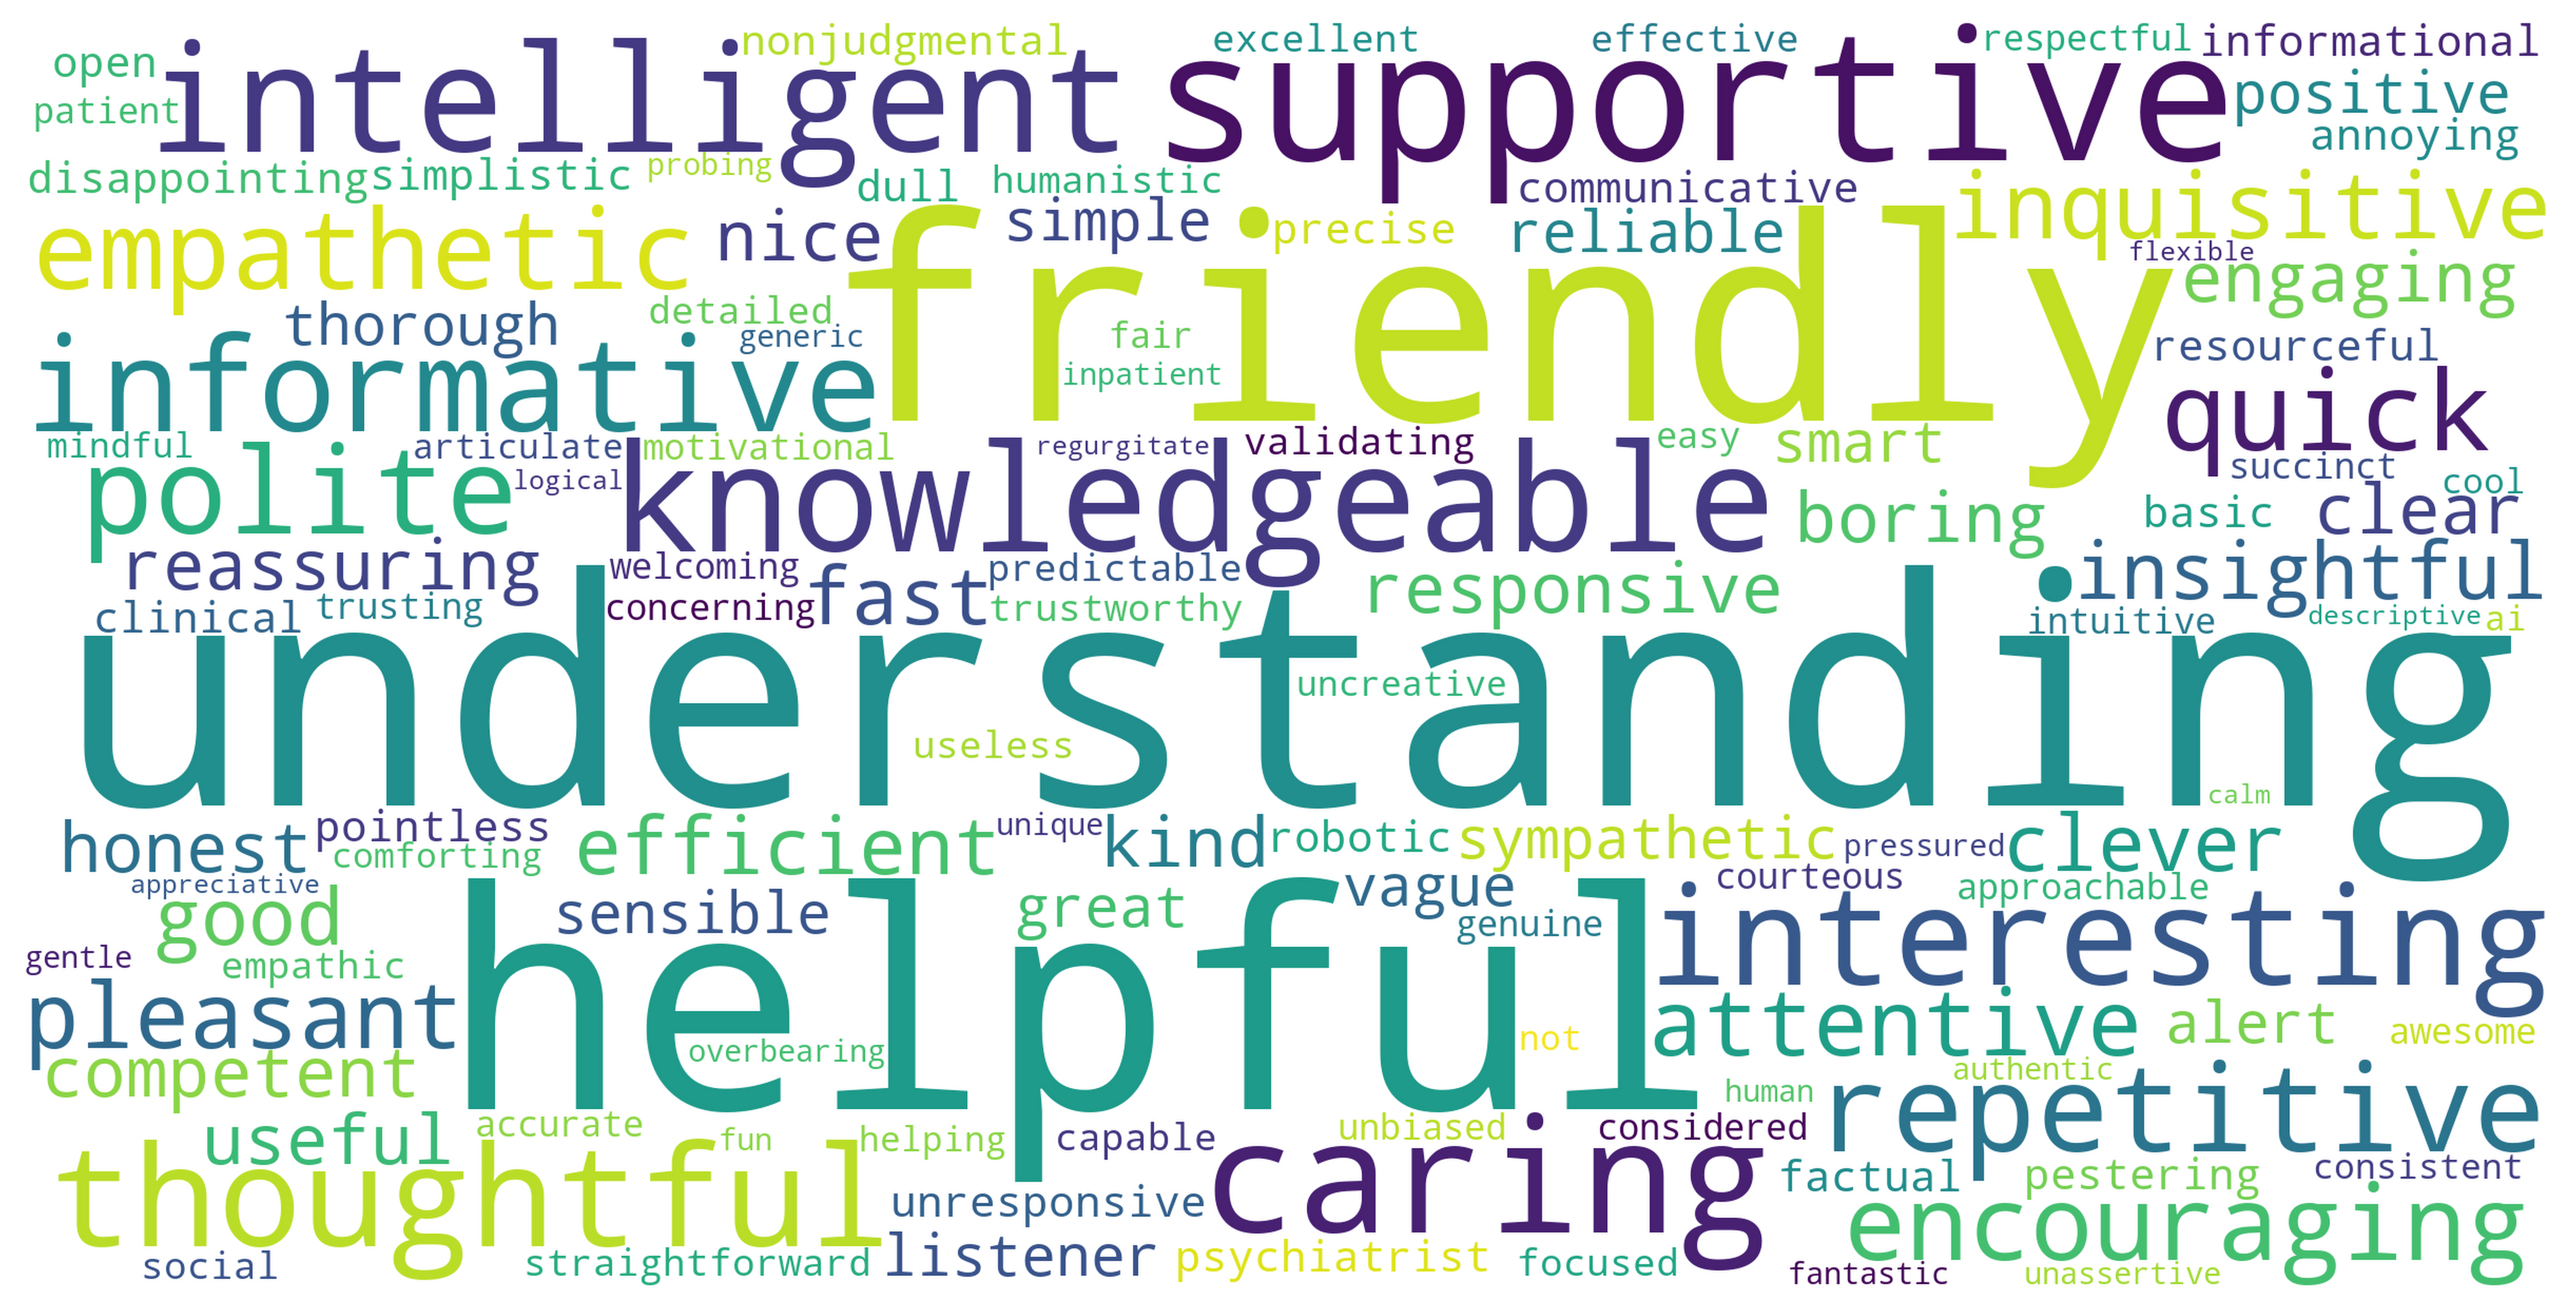
\includegraphics[width=0.9\textwidth]{fig/wordcloud.png}
  \caption{Word cloud representation of participant feedback.}
  \label{word_cloud}
\end{figure*}

\chapter{AutoMISC}
\label{app:automisc}


\Cref{fig:automisc} shows a system flow diagram of AutoMISC. First, each volley (turn of speech) is parsed into one or more utterances (units of thought) by the Parser module. Then, utterance-level annotations, i.e. behavioural codes, are assigned by the Annotator module to each utterance. Up to $k=5$ prior volleys are included in the Annotator module when coding utterances.



\section*{AutoMISC Validation}
\label{appendix:automisc_val}


We present the pairwise Cohen's $\kappa$ values, for both counsellor and client codes, in \Cref{fig:ck}. All $\kappa$ values fall between 0.55-0.81, indicating moderate to substantial agreement between each pair of raters beyond chance~\cite{cohenrange}. The Cohen's $\kappa$ values between AutoMISC and the expert annotators (Annotators 1 and 2) were \textbf{0.63} and \textbf{0.58} for counsellor codes, and \textbf{0.63} and \textbf{0.69} for client codes, respectively.

\section*{Statistical Validation of Inter-Rater Reliability}
To estimate how these reliability findings generalize to more transcripts, we computed the \textbf{asymptotic variance} of Fleiss' $\kappa$ to calculate two-tailed $p$-values. For both counsellor and client codes, the asymptotic variance was on the order of $10^{-6}$, resulting in $p$-values of $p<.001$. These extremely low $p$-values indicate that the inter-rater agreement is highly statistically significant beyond chance. A post-hoc power analysis confirmed that our study was highly powered (estimated power: 1.00) to detect nonzero agreement, i.e., there is a near-certain probability to detect significant inter-rater reliability.

\begin{figure*}[!ht]
	\centering
	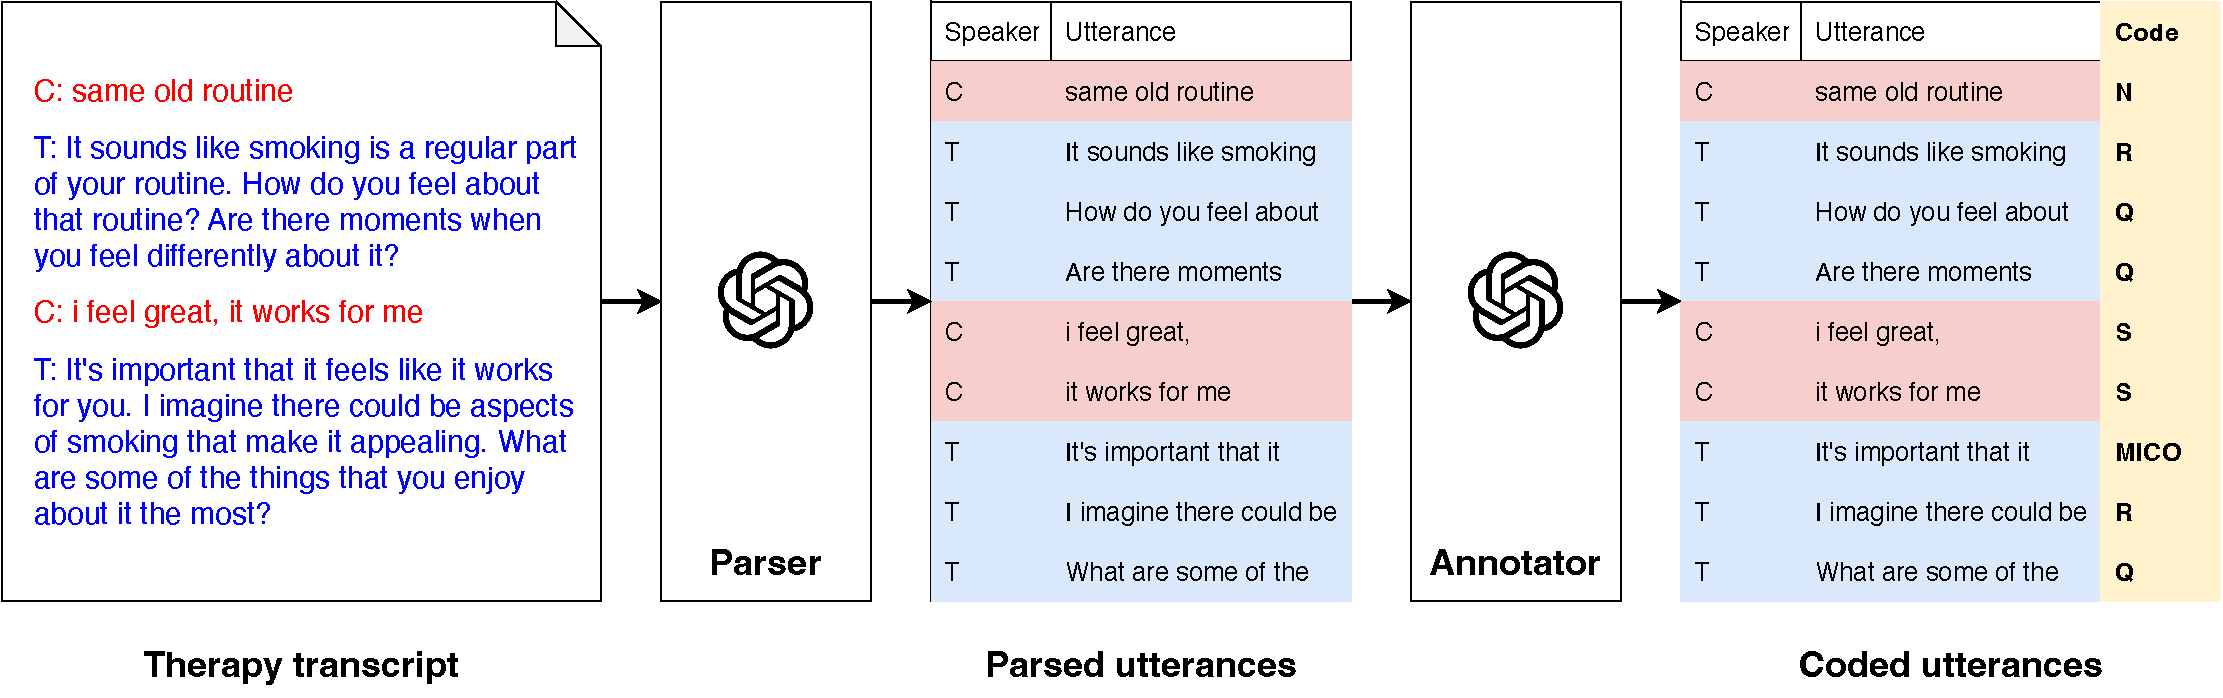
\includegraphics[width=\linewidth]{fig/automisc.pdf}
	\caption[AutoMISC system diagram]{AutoMISC system diagram.}
	\label{fig:automisc}
\end{figure*}

\begin{figure*}[!ht]
	\centering
	\begin{subfigure}[b]{0.48\textwidth}
		\centering
		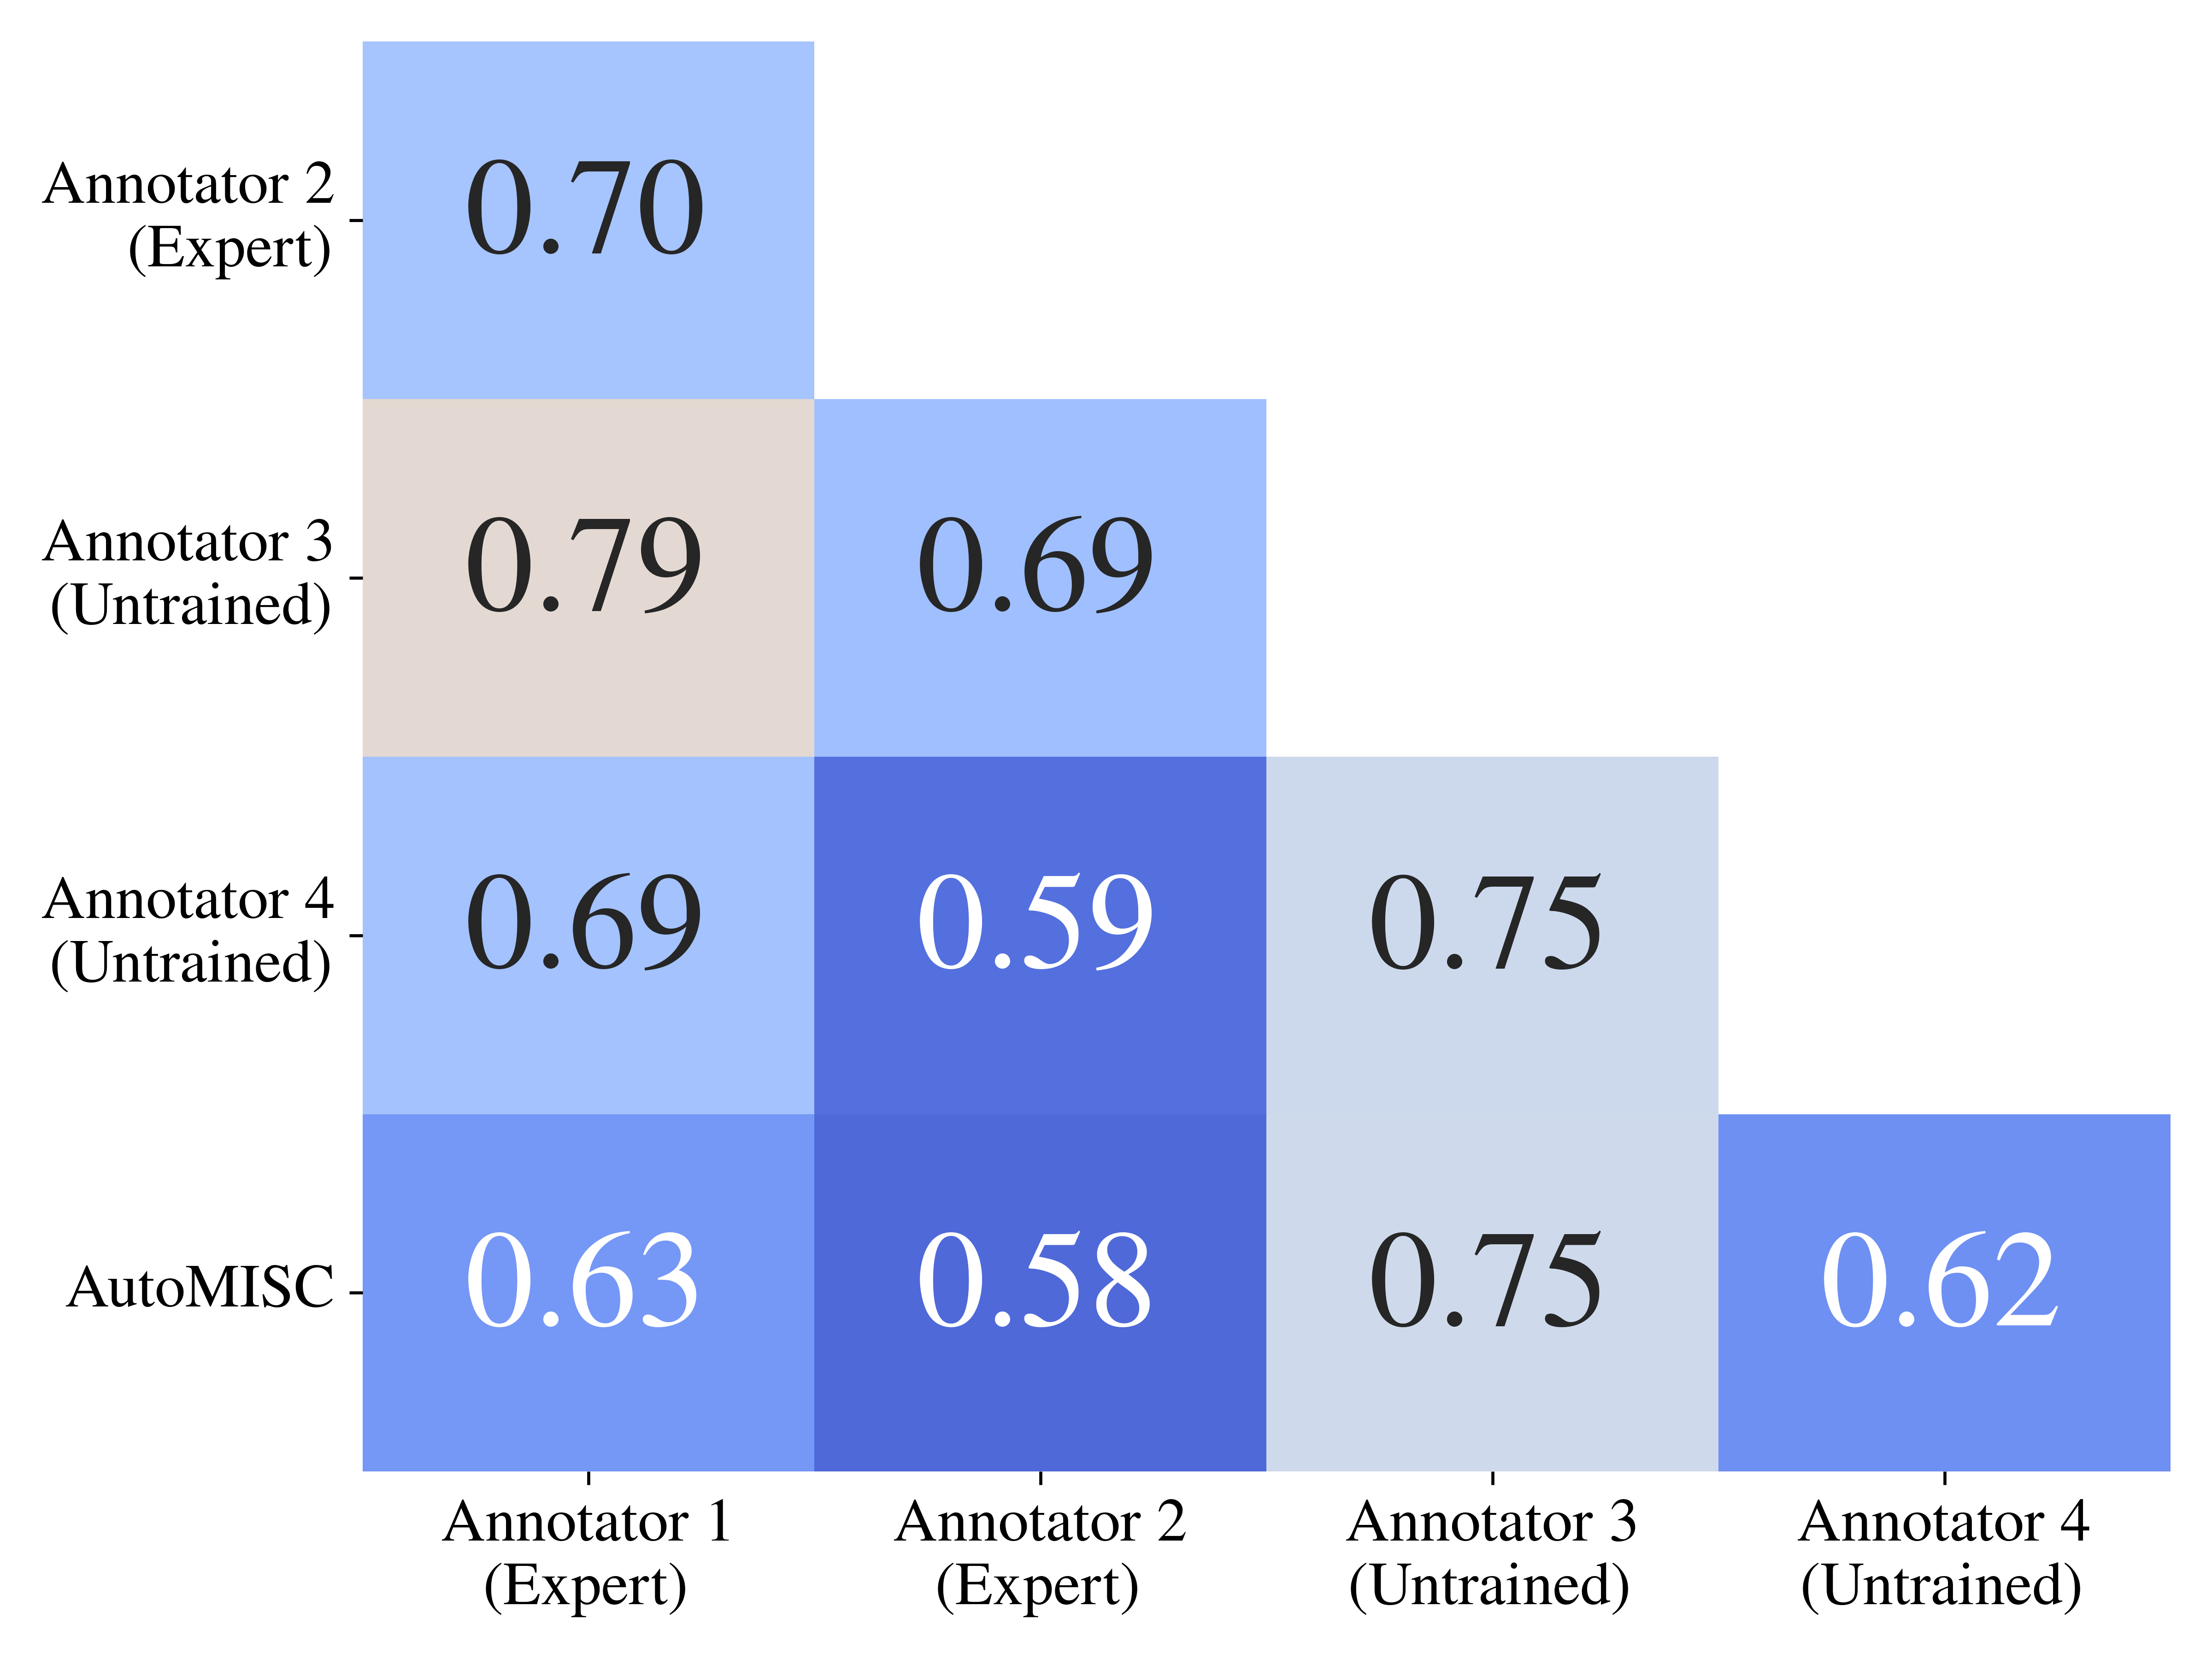
\includegraphics[width=\textwidth]{fig/co_kappa.png}
		\caption{Counsellor codes}
		\label{fig:co_k}
	\end{subfigure}
	\hfill
	\begin{subfigure}[b]{0.48\textwidth}
		\centering
		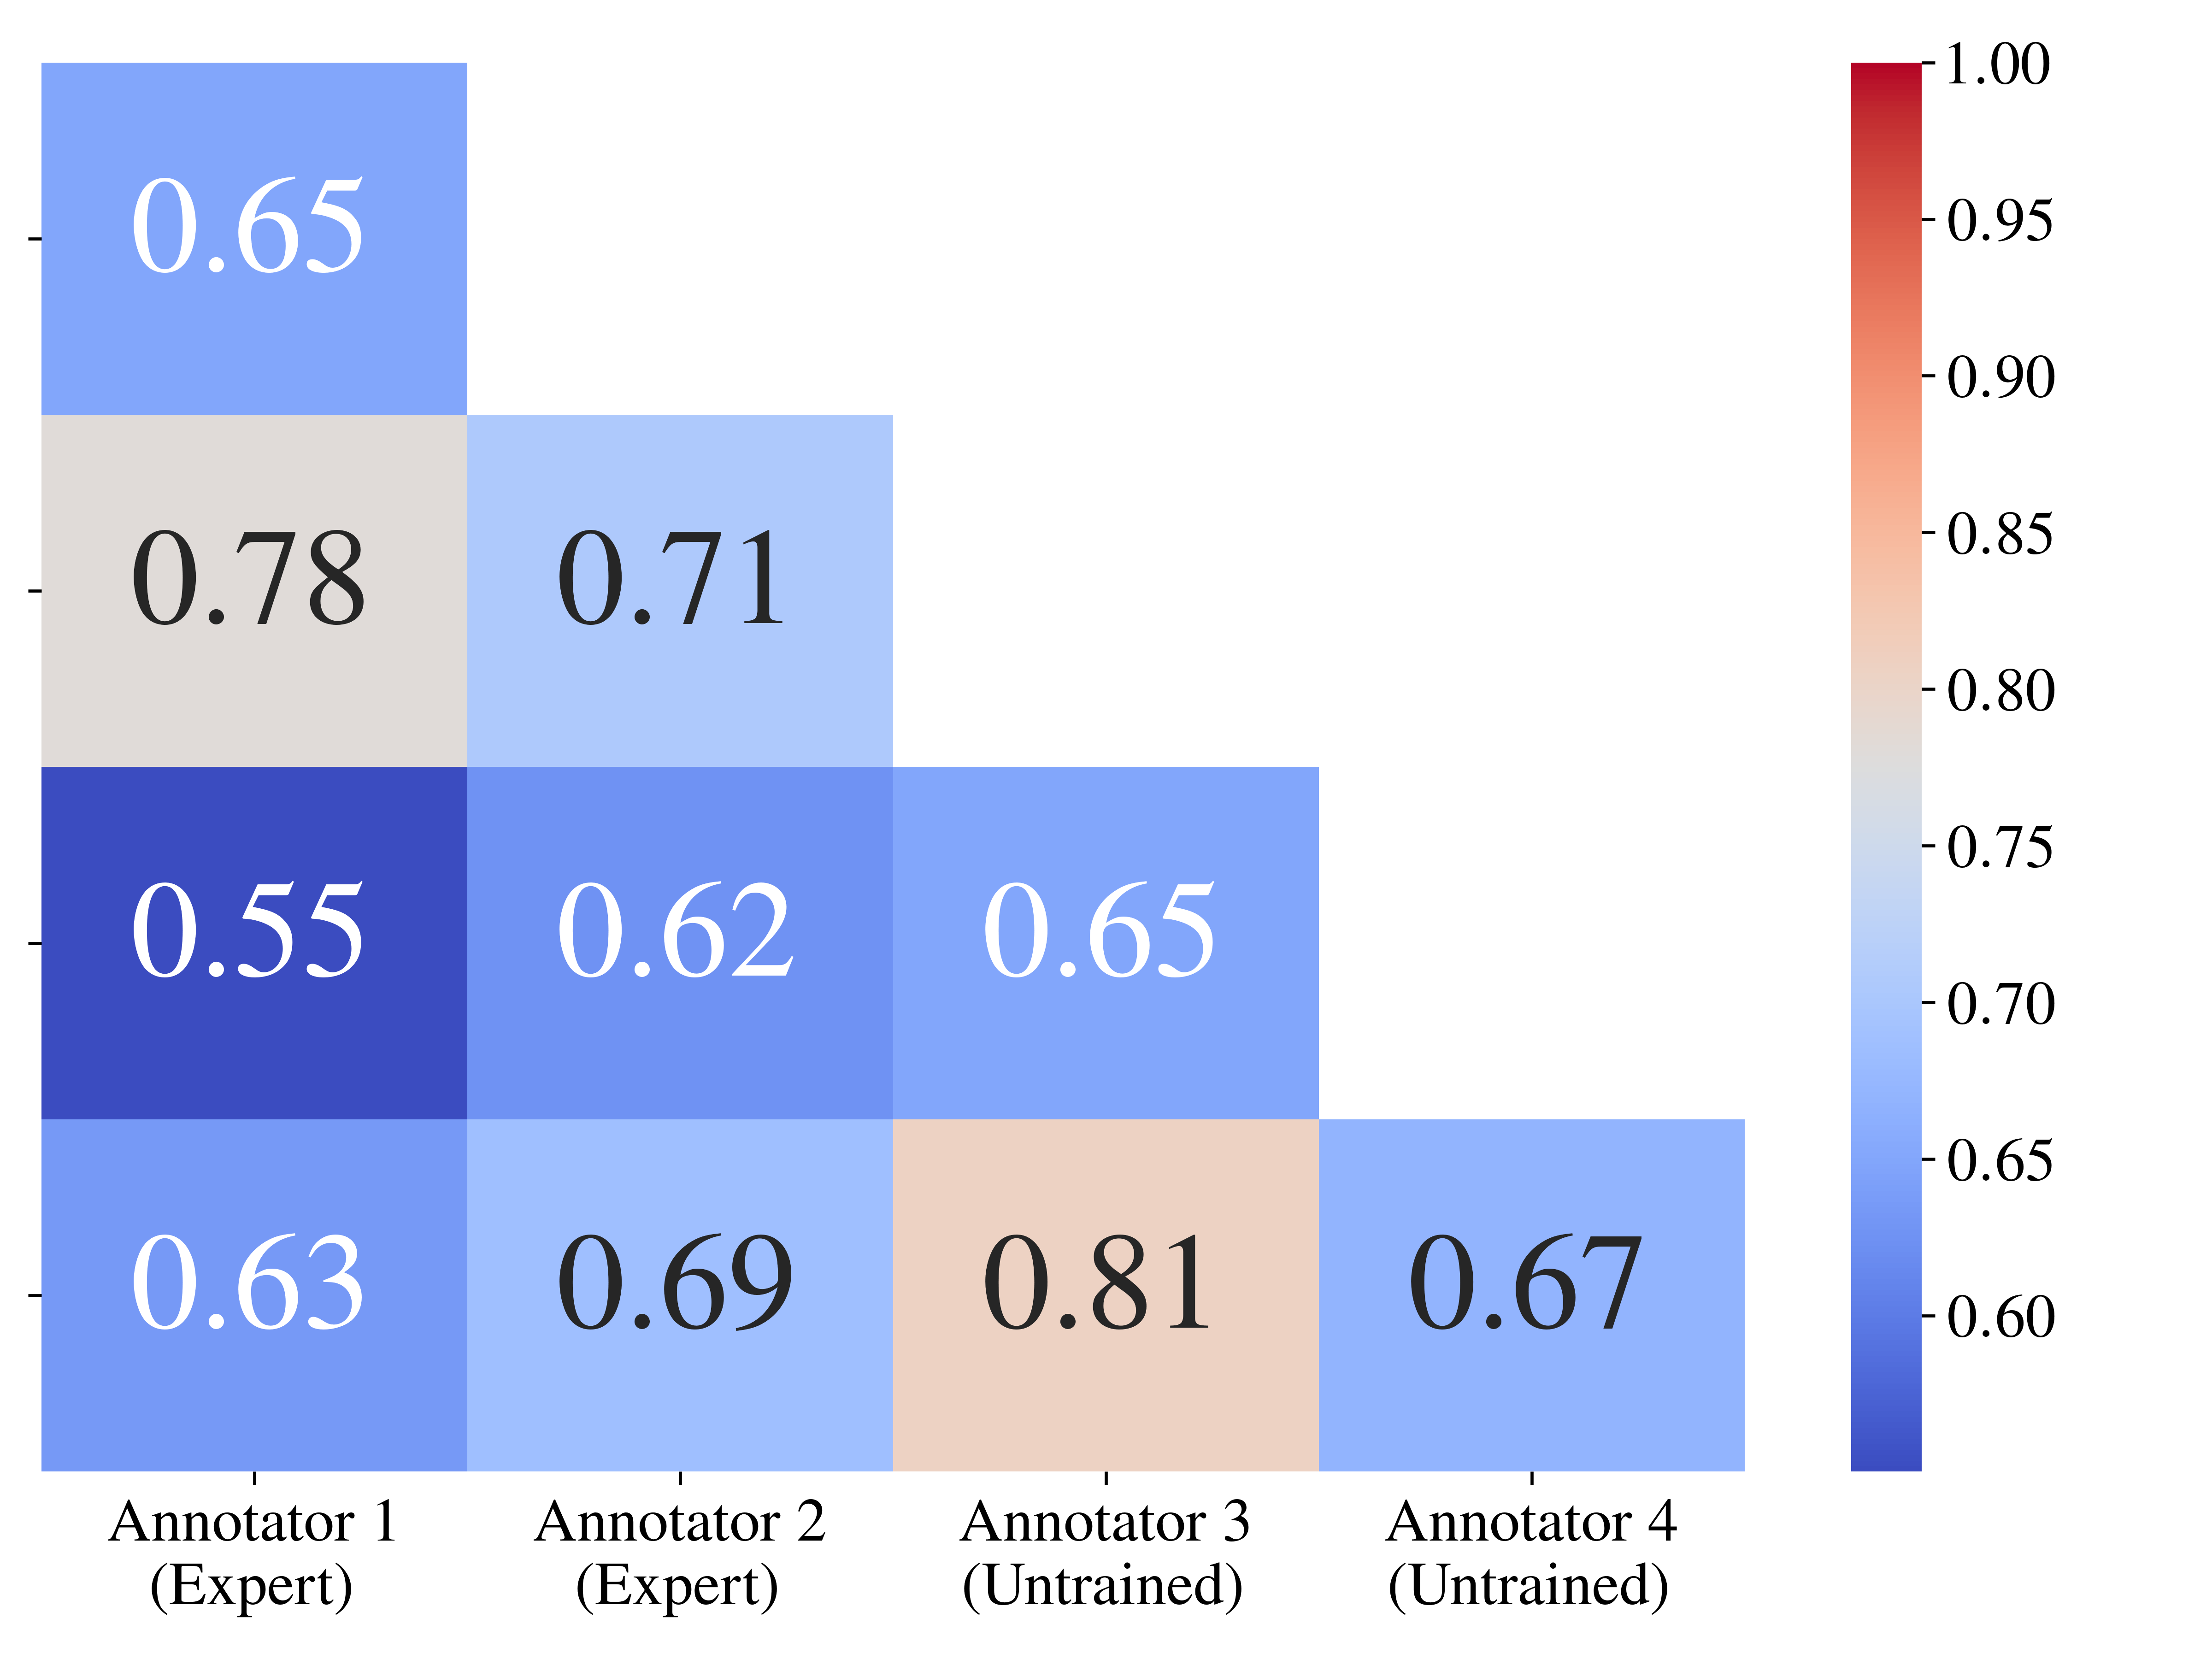
\includegraphics[width=\textwidth]{fig/cl_kappa.png}
		\caption{Client codes}
		\label{fig:cl_k}
	\end{subfigure}
	\caption[Cohen's $\kappa$ between rater pairs on behaviour code annotations]{Cohen's $\kappa$ between rater pairs on behaviour code annotations.}
	\label{fig:ck}
\end{figure*}





\section*{AutoMISC System Prompts}
\label{appendix:automisc_prompts}



\begin{tcolorbox}[
		breakable,
		colback=magenta!5!blue!10,        % Subtle pink/purple background
		colframe=magenta!60!blue!40,      % Darker purple/pink frame
		fontupper=\small,
		title=\subsection*{Parser Prompt}
	]

	You are a highly accurate Motivational Interviewing (MI) counselling session annotator.
	Your task is to segment the given volley into utterances.\\

	Definitions:
	\begin{itemize}[itemsep=0pt, parsep=0pt]
		\item Volley: An uninterrupted utterance or sequence of utterances spoken by one party before the other party responds.
		\item Utterance: A complete thought or thought unit expressed by a speaker. This could be a single sentence, phrase, or even a word if it conveys a standalone idea. Multiple utterances often run together without interruption in a volley.
	\end{itemize}

	Output Format:
	\begin{itemize}[itemsep=0pt, parsep=0pt]
		\item Return the segmented utterances as a Python list of strings.
	\end{itemize}

	Examples:
	Below are examples of how to segment a volley into utterances. Follow this structure when processing new inputs.

	\lstset{
		basicstyle=\ttfamily\small,
		breaklines=true,
		frame=single,
		backgroundcolor=\color{gray!10}
	}
	\begin{lstlisting}
Input:  "Why haven't you quit smoking? Are you ever going to quit?"
Output: ["Why haven't you quit smoking?", "Are you ever going to quit?"]

Input:  "How long since your last drink? Do you feel ok?"
Output: ["How long since your last drink?", "Do you feel ok?"]

Input:  "I can't quit. I just can't do it. I don't have what it takes. I just cannot stop."
Output: ["I can't quit.", "I just can't do it.", "I don't have what it takes.", "I just cannot stop."]

Input:  "I don't want to go to the bars every day. I don't want my kids to see that. I want my kids to have a better life than that."
Output: ["I don't want to go to the bars every day.", "I don't want my kids to see that.", "I want my kids to have a better life than that."]
\end{lstlisting}

\end{tcolorbox}



\begin{tcolorbox}[breakable,
		% width=\textwidth, % Full page width
		colback=magenta!5!blue!10,        % Subtle pink/purple background
		colframe=magenta!60!blue!40,      % Darker purple/pink frame
		fonttitle=\bfseries, % Bold title font
		fontupper=\small,
		title=\subsection*{Counsellor Utterance Classification Prompt}]

	You are a highly accurate Motivational Interviewing (MI) counselling session annotator.
        Your task is to analyze an excerpt from a counselling session of up to five volleys and categorize the counsellor's final utterance.\\

	Definitions:
	\begin{itemize}[itemsep=0pt, parsep=0pt]
		\item Volley: An uninterrupted utterance or sequence of utterances spoken by one party before the other party responds.
		\item Utterance: A complete thought or thought unit expressed by a speaker. This could be a single sentence, phrase, or even a word if it conveys a standalone idea. Multiple utterances often run together without interruption in a volley.
	\end{itemize}

	Task:
	\begin{enumerate}[itemsep=0pt, parsep=0pt]
		\item Determine whether the counsellor's final utterance in the excerpt belongs to one of the following categories:
		      \begin{itemize}[itemsep=0pt, parsep=0pt]
			      \item MI-Consistent (MICO): Directly prescribed in Motivational Interviewing (excluding Reflections and Questions).
			      \item MI-Inconsistent (MIIN): Directly proscribed in Motivational Interviewing principles.
			      \item Reflection or Question (RQ): Includes Reflections or Questions.
			      \item Other (Other): Does not fit the above categories.
		      \end{itemize}
		\item Return your analysis as:
		      \begin{itemize}
			      \item explanation: Briefly justify your choice in one to two sentences.
			      \item label: Provide only MICO, MIIN, RQ, or Other.
		      \end{itemize}
	\end{enumerate}

	Behavioural Code Guide:\\

	MI-Consistent (MICO):
	\begin{itemize}[itemsep=0pt, parsep=0pt]
		\item Affirm (AF): Communicates something positive or complimentary about the client's strengths or efforts.
		\item Advise with permission (ADP): After receiving permission, gives advice, makes a suggestion, or offers a solution or possible action.
		\item Emphasize control (EC): Acknowledges, honors, or emphasizes the client's autonomy and freedom of choice.
		\item Raise concern with permission (RCP): After getting permission, points out a possible problem with a client's goal, plan, or intention. Always phrased as the counsellor's concern.
		\item Support (SU): Sympathetic, compassionate, or understanding comments, which agree or side with the client.
	\end{itemize}

	MI-Inconsistent (MIIN):
	\begin{itemize}[itemsep=0pt, parsep=0pt]
		\item Advise without permission (ADWP): Offers suggestions or guidance without asking or receiving permission.
		\item Confront (CON): Directly disagrees, argues, corrects, shames, blames, seeks to persuade, criticizes, judges, labels, moralizes, ridicules, or questions the client's honesty.
		\item Direct (DIR): Gives an order, command, or direction. The language is imperative.
		\item Raise concern without permission (RCWP): Without getting permission, points out a possible problem with a client's goal, plan, or intention.
		\item Warn (WA): Provides a warning or threat, implying negative consequences unless the client takes a certain action.
	\end{itemize}

	Reflection or Question (RQ):
	\begin{itemize}[itemsep=0pt, parsep=0pt]
		\item Question (Q): Asks a question to gather information, understand, or elicit the client's story.
		\item Reflection (R): Makes a statement that reflects back content or meaning previously offered by the client, usually (but not always) in the client's immediately preceding utterance.
	\end{itemize}

	Other (Other):
	\begin{itemize}[itemsep=0pt, parsep=0pt]
		\item Facilitate (FA): Simple utterance that functions as a ``keep-going'' acknowledgment, e.g., ``Mm-hmm'', ``I see'', ``Go on''.
		\item Filler (FI): Pleasantries such as ``Good morning'', ``Nice weather we're having'', etc.
		\item Giving Information (GI): Provides information to the client, explains something, educates or provides feedback, or discloses personal information.
		\item Structure (ST): Gives information about what will happen directly to the client throughout the course of treatment or within a study format, in this or subsequent sessions.
	\end{itemize}

	Based on the following excerpt, determine which category the counsellor's last utterance falls into and respond accordingly. After you're done, go back over the RQ category and assign a subcategory of ``R'' for reflection or ``Q'' for question.
\end{tcolorbox}



\begin{tcolorbox}[breakable,
		% width=\textwidth, % Full page width
		colback=magenta!5!blue!10,        % Subtle pink/purple background
		colframe=magenta!60!blue!40,      % Darker purple/pink frame
		fonttitle=\bfseries, % Bold title font
		fontupper=\small,
		title=\subsection*{Client Utterance Classification Prompt}]

	You are a highly accurate Motivational Interviewing (MI) counselling session annotator.
        Your task is to analyze an excerpt from a counselling session of up to five volleys and categorize the client's final utterance.
	The target behaviour change of this conversation is smoking cessation.

	Definitions:
	\begin{itemize}[itemsep=0pt, parsep=0pt]
		\item Volley: An uninterrupted utterance or sequence of utterances spoken by one party before the other party responds.
		\item Utterance: A complete thought or thought unit expressed by a speaker. This could be a single sentence, phrase, or even a word if it conveys a standalone idea. Multiple utterances often run together without interruption in a volley.
	\end{itemize}

	Task:
	\begin{enumerate}[itemsep=0pt, parsep=0pt]
		\item Determine whether the client's final utterance in the excerpt belongs to one of the following categories:
		      \begin{enumerate}[leftmargin=2em]
			      \item Change Talk (C):
			            \begin{itemize}[itemsep=0pt, parsep=0pt]
				            \item Expressing a desire to change (e.g., ``I really want to quit smoking'').
				            \item Recognizing the downsides of the current behaviour (e.g., ``My health is suffering because I smoke'').
				            \item Identifying potential benefits of making a change (e.g., ``I would feel better if I exercised more'').
				            \item Demonstrating commitment to change (e.g., ``I'm ready to make a plan to lose weight'').
			            \end{itemize}

			      \item Sustain Talk (S):
			            \begin{itemize}[itemsep=0pt, parsep=0pt]
				            \item Minimizing the problem (e.g., ``It's not that bad, I can handle it'').
				            \item Highlighting difficulties or challenges of change (e.g., ``I don't know if I can give up smoking'').
				            \item Expressing doubts about the ability to change (e.g., ``I've tried to quit before and failed'').
				            \item Focusing on the positive aspects of the current behaviour (e.g., ``Smoking helps me relax'').
			            \end{itemize}

			      \item Neutral Talk (N):
			            \begin{itemize}[itemsep=0pt, parsep=0pt]
				            \item Describing current situations or circumstances without expressing a strong pro- or anti-change stance (e.g., ``I've been thinking about making changes'').
				            \item Asking questions related to the situation or change process (e.g., ``What are the pros and cons of changing?'').
				            \item Making general or factual statements about the issue (e.g., ``It's important to take care of my health'').
			            \end{itemize}
		      \end{enumerate}
		\item Return your analysis as:
		      \begin{itemize}
			      \item explanation: Briefly justify your choice in 1-2 sentences.
			      \item label: Provide only ``C'', ``S'', or ``N''.
		      \end{itemize}
	\end{enumerate}

\end{tcolorbox}
\vspace{1em}
\section*{Demographics of the Annotators}

% \multicollinenumbers
As described in \cref{subsec:automisc}, we enlisted four annotators --- two experts and two novices --- to annotate 10 of the 106 transcripts (comprising 821 utterances) from our study. High alignment between the annotators' labels and the AutoMISC annotations serves as an indicator of AutoMISC's validity. Below, we present their demographic information, following the guidelines proposed by \citet{bender-friedman-2018-data}.


\renewcommand{\arraystretch}{1.1} % optional, if you want extra vertical spacing
% \arrayrulecolor{gray!50}         % adjust the shade of grey as desired

\begin{table}[!ht]
	\centering
	\begin{threeparttable}
		\caption{Demographic Information of Annotators}
		\label{tab:annotator-demographics}
		\begin{tabular}{%
			@{}p{0.25\textwidth}
			p{0.15\textwidth}
			p{0.15\textwidth}
			p{0.15\textwidth}
			p{0.15\textwidth}@{}}
			\toprule
			                                 & \textbf{Annotator \#1\tnote{1}}
			                                 & \textbf{Annotator \#2\tnote{2}}
			                                 & \textbf{Annotator \#3\tnote{3, 4}}
			                                 & \textbf{Annotator \#4\tnote{3, 4}}                                             \\
			\midrule
			\arrayrulecolor{gray!50}
			\textbf{Sex}                     & Female                             & Female    & Male          & Male          \\
			\hline
			\textbf{Age Group (years)}       & 60--69                             & 40-49     & 20-29         & 20-29         \\
			\hline
			\textbf{Race/Ethnicity}          & White                              & White     & Mixed         & Asian         \\
			\hline
			\textbf{Native Language}         & English                            & English   & English       & Mandarin      \\
			\hline
			\textbf{Student Status}          & No                                 & No        & Yes           & Yes           \\
			\hline
			\textbf{Employment Status}       & Full-Time                          & Full-Time & N/A           & N/A           \\
			\hline
			\textbf{Highest Education}       & Graduate                           & Graduate  & Undergraduate & Undergraduate \\
			\hline
			\textbf{Country of Residence}    & Canada                             & Canada    & Canada        & Canada        \\
			\hline
			\textbf{Country of Birth}        & Canada                             & Canada    & Canada        & China         \\
			\hline
			\textbf{Training in Linguistics} & No                                 & No        & No            & No            \\
			\hline
			\textbf{Training in MI}          & Yes                                & Yes       & No            & No            \\
			\arrayrulecolor{black}
			\bottomrule
		\end{tabular}

		\begin{tablenotes}
			\footnotesize
			\item[1]
			Motivational Interviewing Network of Trainers (MINT) member since 2009;
			Motivational Interviewing Treatment Integrity (MITI) coding trained; broad training
			and coaching experience.
			\item[2]
			Introductory-Intermediate-Advance MI training;
			MINT member since 2014;
			MI supervision; MITI training.
			\item[3, 4]
			Engineering graduate student with no formal training in MI.
		\end{tablenotes}

	\end{threeparttable}
\end{table}

\chapter{Deployment Artifacts}
\label{app:deployment-artifacts}

\begin{lstlisting}[language=bash, caption={Dockerfile}, label={lst:dockerfile}]
FROM python:3.11-slim

# Update, install curl for health checks, and clean up
RUN apt-get update && apt-get install -y curl && rm -rf /var/lib/apt/lists/*

WORKDIR /app

# Copy and install dependencies
COPY requirements.txt requirements.txt
RUN pip install --no-cache-dir -r requirements.txt

# Copy application code
COPY app.py app.py
COPY src src

# Expose the port the app runs on
EXPOSE 80

# Define the command to run the application
CMD ["python", "-m", "app"]

# Define the health check
HEALTHCHECK --interval=30s --timeout=5s --start-period=10s --retries=3 \
    CMD curl -f http://localhost/health || exit 1
\end{lstlisting}


\lstset{style=jsonstyle}


\begin{lstlisting}[language=json, caption={ECS Task Definition}, label={lst:json}]
{
    "compatibilities": [
        "EC2",
        "FARGATE"
    ],
    "containerDefinitions": [
        {
            "command": [
                "-m",
                "app"
            ],
            "cpu": 0,
            "entryPoint": [
                "python"
            ],
            "environment": [
                {
                    "name": "...",
                    "value": "..."
                },
                {
                    "name": "...",
                    "value": ..."
                }
            ],
            "essential": true,
            "healthCheck": {
                "command": [
                    "CMD-SHELL",
                    "curl -f http://localhost/health || exit 1"
                ],
                "interval": 300,
                "retries": 4,
                "startPeriod": 20,
                "timeout": 60
            },
            "image": "...amazonaws.com/mibotv6:production",
            "logConfiguration": {
                "logDriver": "awslogs",
                "options": {
                    "awslogs-group": "/ecs/mibot-v6-task",
                    "awslogs-create-group": "true",
                    "awslogs-region": "us-east-2",
                    "awslogs-stream-prefix": "ecs"
                }
            },
            "name": "mibot-v6-container",
            "portMappings": [
                {
                    "appProtocol": "http",
                    "containerPort": 80,
                    "hostPort": 80,
                    "protocol": "tcp"
                }
            ]
        }
    ],
    "cpu": "1024",
    "family": "mibot-v6-task",
    "memory": "4096",
    "networkMode": "awsvpc",
    "revision": 87,
    "status": "ACTIVE"
}
\end{lstlisting}



\begin{table}[ht!]
	\centering


	\begin{tabular}{ll}
		\toprule
		\textbf{Resource Path}            & \textbf{Allowed HTTP Method} \\
		\midrule

		% Use \multirow for cells that span multiple rows.
		% The first argument is the number of rows to span.
		\multirow{2}{*}{/chat}            & POST                         \\
		                                  & OPTIONS                      \\
		\cmidrule(l){2-2} % Adds a small line to separate groups

		\multirow{2}{*}{/get\_transcript} & POST                         \\
		                                  & OPTIONS                      \\
		\cmidrule(l){2-2}

		\multirow{2}{*}{/health}          & GET                          \\
		                                  & OPTIONS                      \\
		\cmidrule(l){2-2}

		\multirow{2}{*}{/info}            & GET                          \\
		                                  & OPTIONS                      \\
		\cmidrule(l){2-2}

		\multirow{2}{*}{/s3\_upload}      & POST                         \\
		                                  & OPTIONS                      \\

		\bottomrule
	\end{tabular}
	\caption{API Gateway Resource and Method Configuration}
	\label{tab:api_gateway}
\end{table}

\chapter{System Architecture Diagram}
\label{app:architecture-diagrams}

\begin{figure}[h!]
	\centering
	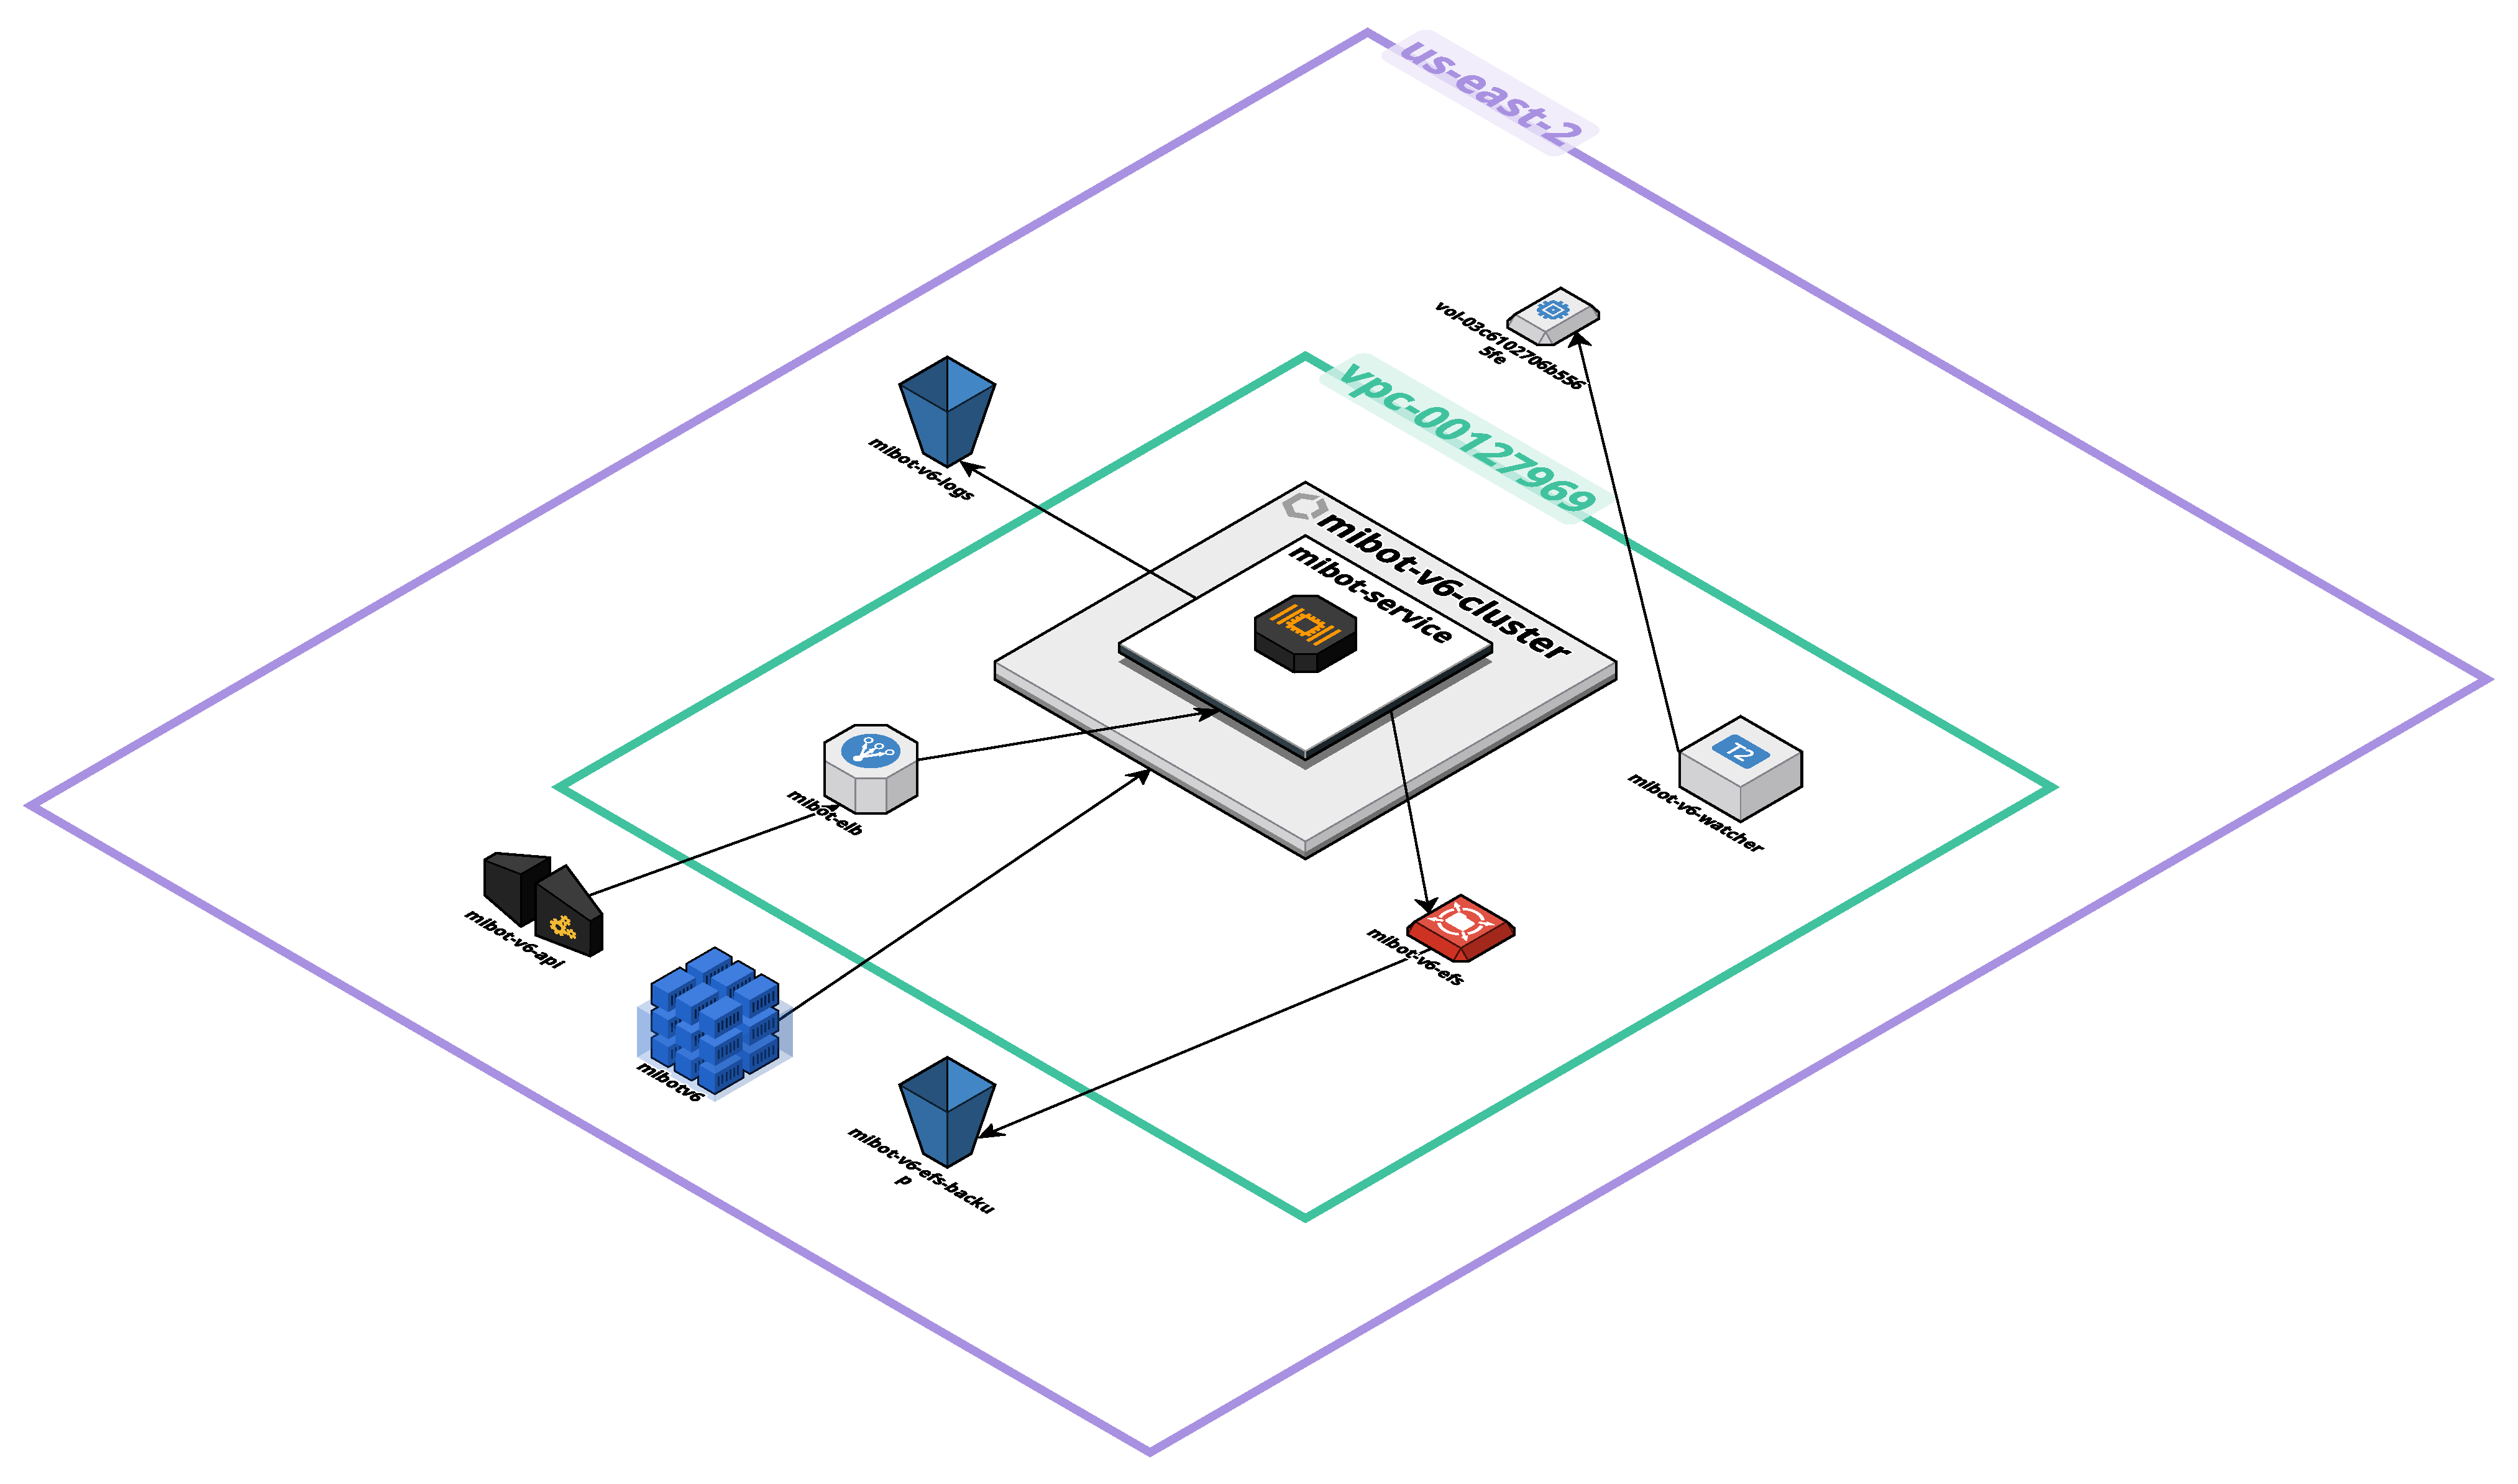
\includegraphics[width=0.99\linewidth]{fig/3bc60efd-554e-416c-87c9-8e19116d1634.pdf}
	\caption{MIBot system architecture}
	\label{fig:mibot-sys-arch}
\end{figure}
\chapter{Overview of the Dataset}
\label{appendix:dataset_overview}

We are releasing the complete data from our feasibility study. Our dataset consists of a CSV file (\texttt{data.csv}), where each row corresponds to a unique participant. A total of 106 participants took part in the study. We also provide conversation transcripts between MIBot and participants in another CSV file (\texttt{conversations.csv}). All data provided by participants has been de-identified using the \texttt{spaCy}\footnote{\url{https://spacy.io/universe/project/scrubadub_spacy}} (version 3.8.4)
and \texttt{scrubadub}\footnote{\url{https://github.com/LeapBeyond/scrubadub}} (version 2.0.0) Python libraries. Further, the participants self-reported all the columns in the dataset (except for AutoMISC annotations). This dataset is licensed under CC BY-SA 4.0\footnote{To view a copy of this license, visit \url{https://creativecommons.org/licenses/by-sa/4.0/}}.

% \vspace{2em}
% {\small
\begin{longtable}{l p{10cm}}
\caption{Description of the Columns in \texttt{data.csv}}\\

\toprule
\textbf{Column Name} & \textbf{Description}\\
\midrule
\endfirsthead

\toprule
\textbf{Column Name (contd.)} & \textbf{Description (contd.)}\\
\midrule
\endhead


\endfoot

\bottomrule
\endlastfoot

\multicolumn{2}{l}{\textbf{Basic}} \\
\texttt{ParticipantId} & Unique participant ID assigned in the study.\\
\midrule


\multicolumn{2}{l}{\textbf{Pre-conversation Survey on Heaviness of Smoking}} \\
\texttt{DailyNum} & How many cigarettes do you typically smoke per day?\\ 
\texttt{FirstCig} & How soon after you wake up do you smoke your first cigarette?\\
\texttt{HeavinessOfSmokingIndex} & Heaviness of Smoking Index~\citep{heatherton1989measuring}\\
\midrule

\multicolumn{2}{l}{\textbf{Pre-conversation Survey on Quit Attempts a Week Prior}} \\
\texttt{PreConvoQuitAttempt} & Have you made any quit attempts (meaning consciously not smoking for a specific period of time greater than 24 hours) during the previous week?\\
\texttt{PreConvoNumQuitAttempts} & How many attempts to quit did you make?\\
\midrule


\multicolumn{2}{l}{\textbf{Pre-conversation Readiness Rulers}} \\
\texttt{PreRulerImportance} & On a scale from 0 to 10, how important is it to you right now to stop smoking?\\
\texttt{PreRulerConfidence} & On a scale from 0 to 10, how confident are you that you would succeed at stopping smoking if you were to start now?\\
\texttt{PreRulerReadiness} & On a scale from 0 to 10, how ready are you to start making a change at stopping smoking right now?\\
\midrule

\multicolumn{2}{l}{\textbf{Post-conversation Readiness Rulers}} \\
\texttt{PostRulerImportance} & On a scale from 0 to 10, how important is it to you right now to stop smoking?\\
\texttt{PostRulerConfidence} & On a scale from 0 to 10, how confident are you that you would succeed at stopping smoking if you were to start now?\\
\texttt{PostRulerReadiness} & On a scale from 0 to 10, how ready are you to start making a change at stopping smoking right now?\\
\midrule

\multicolumn{2}{l}{\textbf{Post-conversation Feedback}} \\
\texttt{FeedbackQ1} & What are three words that you would use to describe the chatbot?\\
\texttt{FeedbackQ2} & What would you change about the conversation?\\
\texttt{FeedbackQ3} & Did the conversation help you realize anything about your smoking behaviour? Why or why not?\\
\texttt{LikedBot} & Whether the participant liked \sysname, based on responses to \texttt{Feedback\-Q1-3}.\\
\texttt{FoundBotHelpful} & Whether the participant found \sysname helpful, based on responses to \texttt{Feedback\-Q1-3}.\\
\midrule

\multicolumn{2}{l}{\textbf{CARE Survey}} \\
\texttt{CAREQ1} & \multirow{3}{*}{See \cref{app:care-survey} for CARE questions.}\\
... & \\
\texttt{CAREQ10} & \\
\midrule



\multicolumn{2}{l}{\textbf{Week Later Readiness Rulers}} \\
\texttt{WeekLaterRulerImportance} & On a scale from 0 to 10, how important is it to you right now to stop smoking?\\
\texttt{WeekLaterRulerConfidence} & On a scale from 0 to 10, how confident are you that you would succeed at stopping smoking if you were to start now?\\
\texttt{WeekLaterRulerReadiness} & On a scale from 0 to 10, how ready are you to start making a change at stopping smoking right now?\\
\midrule

\multicolumn{2}{l}{\textbf{Week Later Quit Attempts}} \\
\texttt{WeekLaterQuitAttempt} & Have you made any quit attempts (meaning consciously not smoking for a specific period of time greater than 24 hours) during the previous week?\\
\texttt{WeekLaterNumQuitAttempts} & How many attempts to quit did you make?\\
\midrule

\multicolumn{2}{l}{\textbf{AutoMISC Labels}} \\
\texttt{AutoMISC\_MICO} & \multirow{11}{*}{See \cref{subsec:automisc} for AutoMISC labels.}\\
\texttt{AutoMISC\_MIIN} &\\
\texttt{AutoMISC\_R} &\\
\texttt{AutoMISC\_Q} &\\
\texttt{AutoMISC\_Other} &\\
\texttt{AutoMISC\_C} &\\
\texttt{AutoMISC\_S} &\\
\texttt{AutoMISC\_N} &\\
\texttt{AutoMISC\_\%MIC} &\\
\texttt{AutoMISC\_R:Q} &\\
\texttt{AutoMISC\_C:S} &\\




% \caption{(Continued)}

\label{tab:datadesc}
\end{longtable}



\vspace{1em}


\begin{table}[ht]
    \centering
    % \small
    \renewcommand{\arraystretch}{1.2}
    \begin{tabular}{l p{10cm}}
        \toprule
        \textbf{Column Name} & \textbf{Description} \\
        \midrule
        \texttt{ParticipantID} & Unique participant ID. \\
        \texttt{Speaker} & Indicates whether the speaker is the \texttt{counsellor} (i.e., \sysname) or the \texttt{client}. \\
        \texttt{Volley\#} & Serial number of the volley in the transcript. ``A volley is an uninterrupted utterance or sequence of utterances by one party, before another party speaks.''~\citep{MISC} \\
        \texttt{Utterance\#} & Serial number of the utterance in the transcript. \\
        \texttt{CumulativeVolley} & Represents the volley up to utterance \# \texttt{Utterance\#}. The \texttt{CumulativeVolley} corresponding to the last utterance of the volley is the complete volley, which can be used to generate the transcript. \\
        \texttt{Utterance} & ``An utterance is a complete thought, or a thought unit.''~\citep{MISC} \\
        \texttt{AutoMISCLabel} & Utterance label according to AutoMISC. It can be one of the following: \texttt{R}, \texttt{Q}, \texttt{Other}, \texttt{C}, \texttt{N}, ... (See \cref{subsec:automisc}.) \\
        \texttt{AutoMISCExplanation} & Explanation provided by the AutoMISC LLM as part of its chain-of-thought. \\
        \bottomrule
    \end{tabular}
    \caption{Description of the Columns in \texttt{conversations.csv}}
    \label{tab:conversations_description}
\end{table}
\chapter{Consent from Participants}
\label{app-consent}


Before participants joined the study, detailed instructions were provided and their consent was obtained to use their data, including survey responses. They were also informed about potential risks. Below are relevant excerpts from the \textbf{Consent Form} that participants were required to read and accept.


\vspace{12pt}

\begin{tcolorbox}[breakable,title=WHAT ARE THE RISKS OR HARM OF PARTICIPATING IN THIS STUDY?]
	This study requires you to think about your smoking habits, which may be stressful for you. Thinking about your smoking habits may temporarily increase your urge to smoke.

	There is a small but very unlikely possibility that the chatbot may generate responses that may provoke the above feelings. Should this happen, you are encouraged to document it in your qualitative feedback opportunity.

	There are no other risks or harm to you in participating in this study.
\end{tcolorbox}

\vspace{12pt}

\begin{tcolorbox}[breakable,title=WHAT COMPENSATION AM I ENTITLED TO?]
	You will be compensated £5.50, or the equivalent in your local currency, for completing the conversation task and £1 for the 1-week later survey.
\end{tcolorbox}

\vspace{12pt}

\begin{tcolorbox}[breakable,title=HOW WILL MY PRIVACY BE RESPECTED?]
	All conversational data and readiness/feedback data recorded during the study will be stored on an encrypted server. The study does not ask you to provide any information that can identify you personally. The original chatbot data collected will only be accessible to the University of Toronto researchers involved with the study.

	Once any personally identifying information has been removed, the conversation may appear in publications or in a public dataset. The data will be used by researchers at the University of Toronto and CAMH to develop chatbots that can have conversations with individuals about their smoking habits. The data will be held by the University of Toronto indefinitely.

	The results of this research study may be presented at meetings or in publications, and this may include direct quotes from your responses and your feedback (after removing any text that personally identifies you), as well as summary statistics from the numerical ratings that all participants provide. In all cases, your identity will not be disclosed.
\end{tcolorbox}

\chapter{Summary of Literature Survey on Synthetic Doppelgängers}
\label{app:lit-review}

{ % Start a group to keep the arrayrulecolor local
\arrayrulecolor{lightgray}
\begin{longtable}{| L{4.5cm} | L{3.5cm} | L{3.5cm} | L{3.5cm} |}

%================== CAPTION AND HEADERS ==================
\caption{Validation Methods for LLM-based Synthetic Subjects}
\label{tab:llm_validation}\\

% --- Header for the first page ---
\hline
\rowcolor{tablehead}
\textbf{Publication} & \textbf{Installation Method} & \textbf{Validation Approach} & \textbf{Limitation of Validation}\\
\hline
\endfirsthead

% --- Header for subsequent pages ---
\hline
\rowcolor{tablehead}
\textbf{Publication} & \textbf{Installation Method} & \textbf{Validation Approach} & \textbf{Limitation of Validation}\\
\hline
\endhead

% --- Footer for all pages except the last ---
\endfoot

% --- Footer for the last page ---
\endlastfoot

%================== TABLE BODY (SORTED BY YEAR) ==================
\citet{andreas-2022-language}. \href{https://aclanthology.org/2022.findings-emnlp.423/}{\textit{Language Models as Agent Models}}. & Not applicable. The paper is a conceptual review and position paper. & The paper synthesizes and reinterprets existing research, using findings from prior literature as evidence for its conceptual claims about agent modeling. & The argument is based on a literature survey and conceptual reasoning, not on novel empirical validation or a quantitative simulation.
\\\hline
\citet{aher2023}. \href{https://proceedings.mlr.press/v202/aher23a.html}{\textit{Using Large Language Models to Simulate Multiple Humans and Replicate Human Subject Studies}}. & Zero-shot prompting of LLMs to simulate participants in replications of classic behavioral experiments (e.g., Ultimatum Game, Milgram experiment). & The paper introduces the 'Turing Experiment' methodology, where the aggregate behavioral distributions of LLM simulations are quantitatively compared to the results of the original human studies. & While the models replicate high-level outcomes, the validation does not guarantee process fidelity. A 'hyper-accuracy distortion' is noted in some models, revealing a non-humanlike bias.
\\\hline
\citet{argyle2023}. \href{https://doi.org/10.1017/pan.2023.2}{\textit{Out of one, many: Using language models to simulate human samples}}. & Conditioning GPT-3 with thousands of socio-demographic backstories from real human survey participants. & Comparison of the response distributions of the "silicon sample" to the human sample to assess "algorithmic fidelity" at the population level. & The validation focuses on aggregate statistical patterns, not on the fidelity of individual-level responses or the realism of conversational interaction.
\\\hline
\citet{ayers2023social}. \href{https://jamanetwork.com/journals/jamainternalmedicine/fullarticle/2804309}{\textit{Comparing Physician and Artificial Intelligence Chatbot Responses to Patient Questions}}. & A chatbot (ChatGPT) and physicians were prompted with real-world patient questions posted on a public social media forum. & A panel of licensed healthcare professionals blindly evaluated the quality and empathy of both human and AI responses. & The Turing-style test focuses on the quality of static, written advice, not on interactive diagnostic capabilities or the ability to manage a longitudinal patient relationship.
\\\hline
\citet{binz2023using}. \href{https://doi.org/10.1073/pnas.2218523120}{\textit{Using cognitive psychology to understand GPT-3}}. & Zero-shot prompting of GPT-3 with classic cognitive bias scenarios (e.g., the Linda problem). & Comparison of the model's pattern of choices and errors against the well-documented results from human experiments. & The validation shows the model reproduces human-like biases in constrained tasks but does not prove the underlying cognitive mechanisms are the same, or that this behavior generalizes to novel tasks.
\\\hline
\citet{he2024agentscourt}. \href{https://arxiv.org/abs/2403.02959}{\textit{AgentsCourt: Building Judicial Decision-Making Agents with Court Debate Simulation and Legal Knowledge Augmentation}}. & Agents are assigned roles (e.g., judge, plaintiff, defendant) and given case evidence to simulate court debates and deliberate a verdict. & Comparison of the LLM jury's final verdict and legal reasoning to the outcomes from human mock jury studies or real-world legal precedents. & The validation focuses on the legal and logical outputs, but fails to model the emotional, social, and group dynamics that heavily influence real jury deliberations.
\\\hline
\citet{gao2023s3}. \href{https://arxiv.org/abs/2307.14984}{\textit{S³: Social-network Simulation System with Large Language Model-Empowered Agents}}. & Agents are instantiated in a social network simulation system (S³) using prompt engineering and tuning to emulate human emotion, attitude, and interaction behaviors. & Evaluation of emergent population-level phenomena (e.g., propagation of information, attitudes, and emotions) against real-world social network data. & The paper describes initial work and focuses on the system's ability to reproduce emergent phenomena, with less emphasis on the micro-level fidelity of individual agent reasoning or behavior.
\\\hline
\citet{horton2023large}. \href{https://www.nber.org/papers/w31122}{\textit{Large Language Models as Simulated Economic Agents: What Can We Learn from Them?}}. & LLMs are instructed to act as players in classic economic games, being given endowments, information, and preferences. & Comparison of LLM decisions to established patterns of human behavior, showing qualitatively similar results to original laboratory experiments. & The validation confirms replication of known qualitative outcomes but does not validate the underlying cognitive processes, suggesting its primary use is for piloting studies, not replacing them.
\\\hline
\citet{kosinski2023evaluating}. \href{https://arxiv.org/abs/2302.02083}{\textit{Evaluating Large Language Models in Theory of Mind Tasks}}. & Zero-shot prompting on classic false-belief tasks. & Performance on standardized psychological tests for Theory of Mind (ToM), comparing newer models (e.g., GPT-4) to older versions and child development benchmarks. & Tests puzzle-solving ability on static, text-based scenarios, which may not equate to genuine social inference or the imputation of mental states in dynamic, real-world interactions.
\\\hline
\citet{alam2023integrating}. \href{https://doi.org/10.3389/fmed.2023.1279707}{\textit{Integrating AI in medical education: embracing ethical usage and critical understanding}}. & Not described (Review paper). & Discusses prevalent validation methods in the field, such as performance on medical exams, user satisfaction, and expert review. & The review highlights a field-wide limitation: a lack of rigorous, comparative validation studies that benchmark AI performance systematically against human experts.
\\\hline
\citet{Park2023}. \href{https://arxiv.org/abs/2304.03442}{\textit{Generative Agents: Interactive Simulacra of Human Behavior}}. & Agents are instantiated with seed memories and personalities via natural language prompts in an interactive sandbox environment. & Ablation studies on agent architecture components and qualitative author evaluation of "believability" of emergent social behaviors. & The validation relies on subjective author assessment of believability and lacks a rigorous, systematic comparison to a quantitative human baseline.
\\\hline
\citet{pmlr-v202-santurkar23a}. \href{https://proceedings.mlr.press/v202/santurkar23a.html}{\textit{Whose Opinions Do Language Models Reflect?}}. & Prompting LLMs with questions from public opinion polls (Pew Research) with and without demographic steering. & Quantitative comparison of the distribution of LM opinions against the responses of 60 U.S. demographic groups using the OpinionQA dataset. & The validation reveals substantial misalignment between LM opinions and U.S. demographic groups, which persists even when the model is explicitly steered toward a target group.
\\\hline
\citet{spatharioti2023comparing}. \href{https://arxiv.org/abs/2307.03744}{\textit{Comparing Traditional and LLM-based Search for Consumer Choice}}. & Participants in a randomized experiment are assigned to use either an LLM-based search tool or a traditional search engine. & Comparison of task completion time, query complexity, user satisfaction, and decision accuracy between the two groups. & Validation shows users with LLMs are faster, but it also reveals a limitation: users exhibit overreliance on the LLM and fail to spot incorrect information when the model errs.
\\\hline
\citet{suh2025language}. \href{https://arxiv.org/abs/2502.16761}{\textit{Language Model Fine-Tuning on Scaled Survey Data for Predicting Distributions of Public Opinions}}. & Fine-tuning LLMs on SubPOP, a large-scale dataset of public opinion survey questions and responses. & Measuring the reduction in the "LLM-human gap" compared to baselines and testing generalization to unseen surveys and subpopulations. & The validation focuses on predicting response distributions from survey data, not on the underlying reasoning or conversational fidelity of the agents.
\\\hline
\citet{laverde2025integrating}. \href{https://doi.org/10.1016/j.csbj.2025.05.025}{\textit{Integrating large language model-based agents into a virtual patient chatbot for clinical anamnesis training}}. & Virtual patients are configured with preset preferences, histories, and personalities via system prompts for medical training simulations. & Evaluation of the consistency and plausibility of agent responses against the defined case, along with a quantitative user satisfaction score from the Chatbot Usability Questionnaire (CUQ). & The validation method is susceptible to evaluator bias and primarily assesses script-following and information retrieval rather than authentic, spontaneous patient behavior.
\\\hline
\citet{jiang-etal-2023-personallm}. \href{https://aclanthology.org/2024.findings-naacl.229/}{\textit{PersonaLLM: Investigating the Ability of Large Language Models to Express Personality Traits}}. & Prompting LLM personas with Big Five personality trait profiles to create "LLM personas." & LLM personas complete the Big Five Inventory (BFI) personality test; human evaluators assess personality from stories written by the personas. & Human accuracy in perceiving the correct personality drops significantly when evaluators are informed of AI authorship, suggesting the perception of personality is fragile.
\\\hline

\end{longtable}
} % End of the \arrayrulecolor scope
\chapter{Example of Attribute Installation in a Doppelgänger}
\label{app:doppelganger-prompts}


\begin{tcolorbox}[breakable,
                  fonttitle=\bfseries, % Bold title font
                  fontupper=\small,
                  title=Example Doppelgänger Prompt]

Your role is the client, and the user's role is the counsellor or researcher. Always try to respond in fewer than 200 characters. \\\\


About you: \\
You are a 31-year-old female. You typically smoke 10 cigarettes per day. After you wake up, you smoke your first cigarette within 5 minutes. In the past week, you have not made any quit attempts.\\
Before speaking to the counsellor, you have rated your motivation to quit as follows (on a scale from 0 to 10): Importance: 3, Confidence: 0, Readiness: 4. Your language should contain approximately 66\% change talk and 34\% sustain talk.
\end{tcolorbox}
\chapter{Full Transcript of a Doppelgänger Interaction}
\label{app:doppelganger-transcript}

% This appendix contains a full, example transcript of a conversation between a doppelgänger and MIBot.


\setupnormalchapters
\backmatter
\addcontentsline{toc}{chapter}{Bibliography}
\printbibliography
\clearpage

\end{document}
